%%%%%%%%%%%%%%%%%%%%%%%%%%%%%%%%%%%%%%%%%%%%%%%%%%%%%%%%%%%

\chapter{Modello del sistema}
\label{ref:modSistema}

%%% Il gruppo 1 scriverà il suo modello del sistema. Esso dovrà includere: attori, casi d'uso (descrizione e tabella), scenari, diagrammi dei casi d'uso, diagrammi di sequenza, diagramma delle attività, screen mockups della funzionalità %%%

\section{Attori}
\label{sec:attori}
\subsection{\textit{Sync}}
\paragraph{} 
\textit{Sync} rappresenta il sincronizzatore remoto, un web service esterno che si interfaccia con una serie di servizi tra cui \textit{Esse3}, ossia il portale dello studente che offre le funzionalità da replicare nell’applicazione, \textit{Aule Unimol} ed altri servizi esterni. È un’entità esterna al sistema che si vuole realizzare, pertanto  è classificata come attore.
\begin{center}
	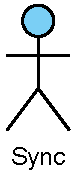
\includegraphics[width=0.6in]{imgs/attori/Attore-Sync.pdf}
\end{center}

\subsection{\textit{Docente}}
\paragraph{} 
\textit{Docente} è un professore dell’\textit{Università degli Studi del Molise} avente le credenziali di accesso al portale \textit{Esse3}. Il \textit{Docente} utilizzerà la nuova funzionalità per comunicare in modo rapido e semplice e anche in via ufficiosa con tutti gli studenti che frequentano un proprio corso. Egli potrà amministrare le chat secondo le sue preferenze, in particolare potrà creare o rimuovere dei canali e aggiungere o rimuovere i membri.
\begin{center}
	
\includegraphics[width=0.6in]{imgs/attori/Docente.png}
\end{center}

\subsection{Studente}
\paragraph{} 
Studente regolarmente iscritto all’\textit{Università degli Studi Del Molise}, munito delle credenziali per accedere al portale dello studente \textit{Esse3}, il servizio esterno sul quale si basa l’applicazione. Lo studente utilizza l’applicazione per usufruire in maniera agevole dei servizi offerti dai portali dell’\textit{Università degli Studi del Molise} e monitorare la propria carriera universitaria. Di seguito è mostrata l'icona dello studente standard.
\begin{center}
	
\includegraphics[width=0.8in]{imgs/attori/Attore-Studente.pdf}
\end{center}
Per quanto riguarda la nuova funzionalità di messaggistica, lo \textit{Studente} utilizzerà tale funzione per facilitare la comunicazione ufficiale con i docenti relativi ai corsi della Coorte di appartenenza. Potrà comunicare, inoltre, con gli altri studenti appartenenti al suo stesso anno di corso. Di seguito è mostrato lo studente della chat.
\begin{center}
	
\includegraphics[width=0.8in]{imgs/attori/Studente.png}
	\label{fig:Attore: Studente chat}
\end{center}

\subsection{Amministratore}
\paragraph{} 
E' un Amministratore dell’\emph{Università degli Studi del Molise}, al quale sono assegnate le credenziali per poter effettuare l’accesso al pannello amministrazione.\emph{L’Amministratore} avrà il compito di gestire, mediante tale pannello, le \emph{chat} degli studenti e le \emph{chat} dei corsi dove potrà coordinare i relativi canali e gli utenti in essi presenti.
Avrà anche la possibilità di inviare notifiche personalizzate e di gestire la segnalazione dei messaggi inopportuni all’interno delle \emph{chat}.

\begin{figure}[h]
	\centering
	
\includegraphics[width=0.2\textwidth]{imgs/attori/admin.png}
	\caption{Attore: Amministratore}
	\label{fig:Attore: Amministratore} 
\end{figure}



\newpage

\section{Scenari}
\subsection{Gestione piano di studio}
\paragraph{Visualizza corsi}
\begin{itemize}
	\item \textit{Visualizzazione avvenuta con successo:}
	Lo studente Giuseppe, iscritto al terzo anno della facoltà di Informatica, accede alla sezione \textit{Piano di studio} per visualizzare i corsi del piano di studio. Nello specifico, per ogni corso il sistema mostra il nome e, se superato, il voto e la data di verbalizzazione:
	\begin{tabbing}
		%La prima riga non viene stampata, serve solo per la spaziatura
		\hspace{1cm}-----------------Esame--------------------------- \= --Voto--- \= --------Data------ \kill
		%Scrivere da qui
		\hspace{1cm} • Programmazione e laboratorio \> 25 \> 01/07/2018 \\
		\hspace{1cm} • Architettura degli elaboratori \> 28 \> 21/01/2018 \\
		\hspace{1cm} • Informatica giuridica \> 30 \> 07/06/2018 \\
		\hspace{1cm} • Matematica \> 24 \> 20/07/2018 \\
		\hspace{1cm} • Basi di dati e sistemi informativi \> 30 \> 15/07/2019 \\
		\hspace{1cm} • Calcolo numerico \> 18 \> 26/03/2019 \\
		\hspace{1cm} • Storia della matematica \> N/D \>\\
		\hspace{1cm} • Informatica territoriale \> N/D \>\\
		\hspace{1cm} • Statistica \> N/D \>\\
		\hspace{1cm} • Intelligenza artificiale \> N/D \>\\
		\hspace{1cm} • Programmazione mobile \> N/D \>\\
	\end{tabbing}
\end{itemize}

\paragraph{Ricerca corsi}
\begin{itemize}
	\item \textit{Ricerca avvenuta con successo:}
	Lo studente Giuseppe, iscritto al terzo anno della facoltà di Informatica, dopo aver visualizzato i corsi del piano di studio, inserisce la parola chiave \textbf{\textit{“Matematica”}}. Il sistema trova i corsi e mostra i risultati:

	\begin{tabbing}
		%La prima riga non viene stampata, serve solo per la spaziatura
		\hspace{1cm}-----------------Esame--------------------------- \= --Voto--- \= --------Data------ \kill
		%Scrivere da qui
		\hspace{1cm} • Matematica \> 24 \> 20/07/2018 \\
		\hspace{1cm} • Storia della matematica \> N/D \>\\
	\end{tabbing}

	\item \textit{La ricerca non restituisce risultati:} 
	Lo studente Giuseppe, iscritto al terzo anno della facoltà di Informatica, dopo aver visualizzato i corsi del piano di studio, inserisce la parola chiave \textbf{\textit{“Matemagica”}}. Il sistema non restituisce alcun riscontro e mostra allo studente il messaggio di errore “Nessun corso trovato”.
\end{itemize}

\paragraph{Filtra corsi con memorizzazione}
\begin{itemize}
	\item \textit{Filtra per anno:} 
	Lo studente Giuseppe, iscritto al terzo anno della facoltà di Informatica, dopo aver visualizzato l’elenco dei corsi del piano di studio, applica il filtro per visualizzare gli esami del \textbf{secondo anno}. Il sistema mostra:
	\begin{tabbing}
		%La prima riga non viene stampata, serve solo per la spaziatura
		\hspace{1cm}-----------------Esame--------------------------- \= --Voto--- \= --------Data------ \kill
		%Scrivere da qui
		\hspace{1cm} • Basi di dati e sistemi informativi \> 30 \> 15/07/2019 \\
		\hspace{1cm} • Calcolo numerico \> 18 \> 26/03/2019 \\
		\hspace{1cm} • Ingegneria del Software\> N/D \> \\
		\hspace{1cm} • Storia della matematica \> 30L \> 04/02/2019 \\
	\end{tabbing}
	
	\item \textit{Filtra esami superati:} 
	Lo studente Giuseppe, iscritto al terzo anno della facoltà di Informatica, dopo aver visualizzato l’elenco dei corsi del piano di studio, applica il filtro per visualizzare gli\textbf{ esami superati}. Il sistema mostra:
	\begin{tabbing}
		%La prima riga non viene stampata, serve solo per la spaziatura
		\hspace{1cm}-----------------Esame--------------------------- \= --Voto--- \= --------Data------ \kill
		%Scrivere da qui
		\hspace{1cm} • Programmazione e laboratorio \> 25 \> 01/07/2018 \\
		\hspace{1cm} • Architettura degli elaboratori \> 28 \> 21/01/2018 \\
		\hspace{1cm} • Informatica giuridica \> 30 \> 07/06/2018 \\
		\hspace{1cm} • Matematica \> 24 \> 20/07/2018 \\
		\hspace{1cm} • Basi di dati e sistemi informativi \> 30 \> 15/07/2019 \\
		\hspace{1cm} • Calcolo numerico \> 18 \> 26/03/2019 \\
	\end{tabbing}
	
	\item \textit{Memorizza filtro:}
	Lo studente Giuseppe, iscritto al terzo anno della facoltà di Informatica, dopo aver visualizzato l’elenco dei corsi del piano di studio ed aver applicato il filtro “esami da sostenere”, sceglie di memorizzarlo. Il sistema mantiene il filtro memorizzato anche in seguito alla chiusura del sistema. Alla successiva apertura dell’app, il sistema filtra di default i corsi per “esami da sostenere”.
	
	\item \textit{Nessuna memorizzazione:}
	Lo studente Giuseppe, iscritto al terzo anno della facoltà di Informatica, dopo aver visualizzato l’elenco dei corsi del piano di studio ed aver applicato il filtro “esami da sostenere”, sceglie di non memorizzare le opzioni inserite. Il sistema applica il filtro selezionato fino alla chiusura del sistema. Alla successiva apertura dell'applicazione, il sistema mostra a Giuseppe tutti i corsi del piano di studio.
	
	\item \textit{Il filtraggio non restituisce alcun risultato:}
	Lo studente Giuseppe, iscritto al terzo anno della facoltà di Informatica, dopo aver visualizzato i corsi del piano di studio, applica il filtro “esami da sostenere” che non restituisce alcun risultato. Il sistema mostra allo studente il messaggio di errore “Nessun esame è stato trovato. Si prega di resettare le impostazioni precedentemente inserite!”
\end{itemize}

\paragraph{Ordina corsi con memorizzazione}
\begin{itemize}
	\item \textit{Ordinamento alfabetico crescente:}
	Lo studente Giuseppe iscritto al terzo anno della facoltà di Informatica, dopo aver visualizzato l'elenco dei corsi del piano di studio, applica l'ordinamento in modo crescente della configurazione in base all’nome del corso. Il sistema mostra:
	\begin{tabbing}
		%La prima riga non viene stampata, serve solo per la spaziatura
		\hspace{1cm}-----------------Esame--------------------------- \kill
		%Scrivere da qui
		\hspace{1cm} • Architettura degli elaboratori \\
		\hspace{1cm} • Basi di dati e sistemi informativi \\
		\hspace{1cm} • Calcolo numerico \\
		\hspace{1cm} • Informatica giuridica \\
		\hspace{1cm} • Matematica \\
		\hspace{1cm} • Programmazione e laboratorio \\
		\hspace{1cm} • Storia della matematica \\
	\end{tabbing}
	
	\item \textit{Ordinamento alfabetico decrescente:}
	Lo studente Giuseppe iscritto al terzo anno della facoltà di Informatica, dopo aver visualizzato l'elenco dei corsi del piano di studio, applica l'ordinamento in modo decrescente della configurazione in base all’nome del corso. Il sistema mostra:
	\begin{tabbing}
		%La prima riga non viene stampata, serve solo per la spaziatura
		\hspace{1cm}-----------------Esame---------------------------\kill
		%Scrivere da qui
		\hspace{1cm} • Storia della matematica \\
		\hspace{1cm} • Programmazione e laboratorio \\
		\hspace{1cm} • Matematica \\
		\hspace{1cm} • Informatica giuridica \\
		\hspace{1cm} • Calcolo numerico \\
		\hspace{1cm} • Basi di dati e sistemi informativi \\
		\hspace{1cm} • Architettura degli elaboratori \\
	\end{tabbing}
	
	\item \textit{Ordinamento per anno crescente:}
	Lo studente Giuseppe iscritto al terzo anno della facoltà di Informatica, dopo aver visualizzato l'elenco dei corsi del piano di studio, applica l'ordinamento in modo crescente della configurazione in base all’anno. Il sistema mostra:
	\begin{tabbing}
		%La prima riga non viene stampata, serve solo per la spaziatura
		\hspace{1cm}-----------------Esame--------------------------- \= ---Anno--- \kill
		%Scrivere da qui
		\hspace{1cm} • Programmazione e laboratorio \> Primo anno\\
		\hspace{1cm} • Matematica  \>Primo anno\\
		\hspace{1cm} • Architettura degli elaboratori \> Primo anno\\
		\hspace{1cm} • Fisica \> Secondo anno\\
		\hspace{1cm} • Calcolo numerico \> Secondo anno\\
		\hspace{1cm} • Intelligenza artificiale \> Terzo anno\\
	\end{tabbing}
	
	\item \textit{Ordinamento per anno decrescente:}
	Lo studente Giuseppe iscritto al terzo anno della facoltà di Informatica, dopo aver visualizzato l'elenco dei corsi del piano di studio, applica l'ordinamento in modo decrescente della configurazione in base all’anno. Il sistema mostra:
	\begin{tabbing}
		%La prima riga non viene stampata, serve solo per la spaziatura
		\hspace{1cm}-----------------Esame--------------------------- \= ---Anno--- \kill
		%Scrivere da qui
		\hspace{1cm} • Intelligenza artificiale \> Terzo anno\\
		\hspace{1cm} • Calcolo numerico \> Secondo anno\\
		\hspace{1cm} • Fisica \> Secondo anno\\
		\hspace{1cm} • Architettura degli elaboratori \> Primo anno\\
		\hspace{1cm} • Matematica  \>Primo anno\\
		\hspace{1cm} • Programmazione e laboratorio \> Primo anno\\
	\end{tabbing}
	
	\item \textit{Ordinamento per CFU crescente:}
	Lo studente Giuseppe iscritto al terzo anno della facoltà di Informatica, dopo aver visualizzato l'elenco dei corsi del piano di studio, applica l'ordinamento in modo crescente della configurazione in base ai CFU. Il sistema mostra:
	\begin{tabbing}
		%La prima riga non viene stampata, serve solo per la spaziatura
		\hspace{1cm}-----------------Esame--------------------------- \= ---CFU--- \kill
		%Scrivere da qui
		\hspace{1cm} • Inglese \> 6 CFU\\
		\hspace{1cm} • Calcolo numerico  \>6 CFU\\
		\hspace{1cm} • Architettura degli elaboratori \> 6 CFU\\
		\hspace{1cm} • Fisica \> 7 CFU\\
		\hspace{1cm} • Intelligenza artificiale \> 9 CFU\\
		\hspace{1cm} • Matematica \> 12CFU\\
	\end{tabbing}
	
	\item \textit{Ordinamento per CFU decrescente:}
	Lo studente Giuseppe iscritto al terzo anno della facoltà di Informatica, dopo aver visualizzato l'elenco dei corsi del piano di studio, applica l'ordinamento in modo decrescente della configurazione in base ai CFU. Il sistema mostra:
	\begin{tabbing}
		%La prima riga non viene stampata, serve solo per la spaziatura
		\hspace{1cm}-----------------Esame--------------------------- \= ---CFU--- \kill
		%Scrivere da qui
		\hspace{1cm} • Matematica \> 12CFU\\
		\hspace{1cm} • Intelligenza artificiale \> 9 CFU\\
		\hspace{1cm} • Fisica \> 7 CFU\\
		\hspace{1cm} • Architettura degli elaboratori \> 6 CFU\\
		\hspace{1cm} • Calcolo numerico  \>6 CFU\\
		\hspace{1cm} • Inglese \> 6 CFU\\
	\end{tabbing}
	
	\item \textit{Ordinamento per voto crescente:}
	Lo studente Giuseppe iscritto al terzo anno della facoltà di Informatica, dopo aver visualizzato l'elenco dei corsi del piano di studio, applica l'ordinamento in modo crescente della configurazione in base al voto. Il sistema mostra:
	\begin{tabbing}
		%La prima riga non viene stampata, serve solo per la spaziatura
		\hspace{1cm}-----------------Esame--------------------------- \= ---Voto--- \kill
		%Scrivere da qui
		\hspace{1cm} • Calcolo numerico \> 18\\
		\hspace{1cm} • Matematica   \>24\\
		\hspace{1cm} • Programmazione e laboratorio \> 25\\
		\hspace{1cm} • Architettura degli elaboratori \> 28\\
		\hspace{1cm} • Informatica giuridica \> 30\\
		\hspace{1cm} • Storia della matematica \> 30L\\
	\end{tabbing}
	
	\item \textit{Ordinamento per voto decrescente:}
	Lo studente Giuseppe iscritto al terzo anno della facoltà di Informatica, dopo aver visualizzato l'elenco dei corsi del piano di studio, applica l'ordinamento in modo decrescente della configurazione in base al voto. Il sistema mostra:
	\begin{tabbing}
		%La prima riga non viene stampata, serve solo per la spaziatura
		\hspace{1cm}-----------------Esame--------------------------- \= ---Voto--- \kill
		%Scrivere da qui
		\hspace{1cm} • Storia della matematica \> 30L\\
		\hspace{1cm} • Informatica giuridica \> 30\\
		\hspace{1cm} • Architettura degli elaboratori \> 28\\
		\hspace{1cm} • Programmazione e laboratorio \> 25\\
		\hspace{1cm} • Matematica \>24\\
		\hspace{1cm} • Calcolo numerico \> 18\\
	\end{tabbing}
	
	\item \textit{Memorizza ordinamento:}
	Lo studente Giuseppe, iscritto al terzo anno della facoltà di Informatica, dopo aver visualizzato l’elenco dei corsi del piano di studio ed aver applicato un ordinamento, sceglie di memorizzare le sue preferenze di ordinamento. Alla successiva apertura dell’applicazione, il sistema ordina i corsi sulla base dell'ultimo ordinamento memorizzato.
	
	\item \textit{Nessuna memorizzazione:}
	Lo studente Giuseppe, iscritto al terzo anno della facoltà di Informatica, dopo aver visualizzato l’elenco dei corsi del piano di studio ed aver applicato un ordinamento, sceglie di non memorizzare le sue preferenze di ordinamento. Il sistema mostra allo studente il messaggio “Le impostazioni non sono state salvate”. 
\end{itemize}

\subsection{Dettagli corso}
\paragraph{Visualizza dettagli corso}
\begin{itemize}
	\item \textit{Visualizzazione dettagli di un corso superato:}
	Lo studente Giuseppe, iscritto al terzo anno della facoltà di Informatica, sceglie di visualizzare i dettagli del corso superato di Informatica giuridica. Il sistema mostra allo studente i seguenti dettagli:
	\begin{tabbing}
		%La prima riga non viene stampata, serve solo per la spaziatura
		\hspace{1cm}-----------------info1--------------------------- \= --inforegistrata1--- \= --info2--\=--inofregistarta2 \kill
		%Scrivere da qui
		\hspace{1cm} • \textbf{Descrizione} Informatica giuridica \> \textbf{Docente} Troncarelli Barbara\\
		\hspace{1cm} • \textbf{Anno} 1 \> \textbf{CFU} 6   \\
		\hspace{1cm} • \textbf{Data esame} 19/06/2018 \> \textbf{Voto} 25 \\
	\end{tabbing}

	\item \textit{Visualizzazione dettagli di un corso non superato:}
	Lo studente Giuseppe, iscritto al terzo anno della facoltà di Informatica, sceglie di visualizzare i dettagli del corso non superato di Ingegneria del software. Il sistema mostra allo studente i seguenti dettagli:
	\begin{tabbing}
		%La prima riga non viene stampata, serve solo per la spaziatura
		\hspace{1cm}-----------------info1--------------------------- \= --inforegistrata1--- \= --info2--\=--inofregistarta2 \kill
		%Scrivere da qui
		\hspace{1cm} • \textbf{Descrizione} Matematica \> \textbf{Docente} Giovanni  Capobianco\\
		\hspace{1cm} • \textbf{Anno} 1 \> \textbf{CFU} 12  \\
	\end{tabbing}
\end{itemize}

\subsection{Gestione appelli}
\paragraph{Visualizza appelli disponibili}
\begin{itemize}
	\item \textit{Visualizzazione avvenuta con successo:}
	Lo studente Giuseppe, iscritto al terzo anno della facoltà di Informatica, sceglie di visualizzare gli appelli disponibili. Il sistema mostra:
	\begin{tabbing}
		%La prima riga non viene stampata, serve solo per la spaziatura
		\hspace{1cm}-----------------info1--------------------------- \= --inforegistrata1--- \= --info2--\=--inofregistarta2 \kill
		%Scrivere da qui
		\hspace{1cm} • \textbf{Descrizione} Basi di dati \> \textbf{Docente} Pareschi Remo
		\\
		\hspace{1cm} •  \textbf{CFU} 12  \> \textbf{Data} 15/06/2019 \\
	\end{tabbing}
	
	\item \textit{Nessun appello disponibile:}
	Lo studente Giuseppe, iscritto al terzo anno della facoltà di Informatica, sceglie di visualizzare gli appelli disponibili. Il sistema non restituisce alcun appello disponibile e mostra il messaggio di errore “Nessun appello disponibile”.
\end{itemize}

\paragraph{Visualizza appelli prenotati}
\begin{itemize}
	\item \textit{Visualizzazione avvenuta con successo:}
	Lo studente Giuseppe, iscritto al terzo anno della facoltà di Informatica, visualizza gli appelli prenotati. Il sistema mostra i dati relativi agli appelli prenotati: 
	\begin{tabbing}
		%La prima riga non viene stampata, serve solo per la spaziatura
		\hspace{1cm}-----------------esame---------------------------\=--Data---\= --tipologia--\kill
		%Scrivere da qui
		\hspace{1cm} • Fisica \> 01/03/2019 \> \hspace{1cm}Orale \\
	\end{tabbing}
	
	\item \textit{Nessun appello prenotato:}
	Lo studente Giuseppe, iscritto al terzo anno della facoltà di Informatica, visualizza gli appelli prenotati. Il sistema non restituisce alcun appello prenotato e mostra il messaggio di errore “Nessun appello prenotato”. 
\end{itemize}

\paragraph{Ricerca appelli disponibili}
\begin{itemize}
	\item \textit{Ricerca avvenuta con successo:}
	Lo studente Giuseppe, iscritto al terzo anno della facoltà di Informatica, dopo aver visualizzato gli appelli disponibili, inserisce la parola chiave \textbf{\textit{“Matematica”}}. Il sistema trova gli appelli disponibili e mostra i risultati:
	\begin{tabbing}
		%La prima riga non viene stampata, serve solo per la spaziatura
		\hspace{1cm}-----------------esame---------------------------\=--Data---\kill
		%Scrivere da qui
		\hspace{1cm} • Matematica  \> 16/02/2019  \\
		\hspace{1cm} • Storia della Matematica \> 18/01/2019 \\
	\end{tabbing}
	
	\item \textit{La ricerca non restituisce risultati:}
	Lo studente Giuseppe, iscritto al terzo anno della facoltà di Informatica, dopo aver visualizzato gli appelli disponibili, inserisce la parola chiave \textbf{\textit{“Matemagica”}}. Il sistema non restituisce alcun riscontro e mostra allo studente il messaggio di errore “Nessun appello trovato”.
\end{itemize}

\paragraph{Filtra appelli disponibili con memorizzazione}
\begin{itemize}
	\item \textit{Filtra per tipologia d’esame (scritto):}
	Lo studente Giuseppe, iscritto al terzo anno della facoltà di Informatica, dopo aver visualizzato l’elenco degli appelli disponibili, sceglie di filtrare gli esami per tipologia \textbf{“scritto”}. Il sistema mostra:  
	\begin{tabbing}
		%La prima riga non viene stampata, serve solo per la spaziatura
		\hspace{1cm}-----------------esame---------------------------\=--Data---\= --tipologia--\kill
		%Scrivere da qui
		\hspace{1cm} • Calcolo numerico  \> 26/03/2019 \> \hspace{1cm}Scritto \\
		\hspace{1cm} • Ingegneria del Software \> 01/04/2019 \> \hspace{1cm}Scritto-Orale  \\
	\end{tabbing}
	
	\item \textit{Filtra per tipologia d’esame (orale):}
	Lo studente Giuseppe, iscritto al terzo anno della facoltà di Informatica, dopo aver visualizzato l’elenco degli appelli disponibili, sceglie di filtrare gli appelli per tipologia di esame \textbf{“orale”}. Il sistema mostra:
	\begin{tabbing}
		%La prima riga non viene stampata, serve solo per la spaziatura
		\hspace{1cm}-----------------esame---------------------------\=--Data---\= --tipologia--\kill
		%Scrivere da qui
		\hspace{1cm} • Informatica giuridica  \> 10/04/2019\> \hspace{1cm}Orale \\
		\hspace{1cm} • Matematica\> 18/04/2019 \> \hspace{1cm}Orale-Scritto  \\
	\end{tabbing}
	
	\item \textit{Filtra per anno:}
	Lo studente Giuseppe, iscritto al terzo anno della facoltà di Informatica, dopo aver visualizzato l’elenco degli appelli disponibili, sceglie di filtrare in base all'anno in cui è previsto il corso e sceglie di filtrare gli appelli per visualizzare solo quelli afferenti al \textbf{secondo anno}. Il sistema mostra:
	\begin{tabbing}
		%La prima riga non viene stampata, serve solo per la spaziatura
		\hspace{1cm}-----------------Esame--------------------------- \= --Voto--- \= --------Data------ \kill
		%Scrivere da qui
		\hspace{1cm} • Basi di dati e sistemi informativi \> 30 \> 15/07/2019 \\
		\hspace{1cm} • Calcolo numerico \> 18 \> 26/06/2019 \\
		\hspace{1cm} • Fisica \> 28 \> 29/06/2019 \\
		\hspace{1cm} • Ingegneria del Software \> N/D \> 7/06/2019  \\
	\end{tabbing}
	
	\item \textit{Memorizza filtro:}
	Lo studente Giuseppe, iscritto al terzo anno della facoltà di Informatica, dopo aver visualizzato l’elenco degli appelli disponibili ed aver applicato il filtro “anno”, sceglie di memorizzarlo. Il sistema mantiene il filtro memorizzato anche in seguito alla chiusura del sistema . Alla successiva apertura dell’app, il sistema filtra di default gli appelli per “anno”.
	
	\item \textit{Nessuna memorizzzazione:}
	Lo studente Giuseppe, iscritto al terzo anno della facoltà di Informatica, dopo aver visualizzato l’elenco degli appelli disponibili ed aver applicato un filtro, sceglie di non memorizzare le opzioni inserite. Alla successiva apertura dell'applicazione, il sistema mostra a Giuseppe tutti gli appelli disponibili.
	
	\item \textit{Il filtraggio non restituisce alcun risultato:}
	Lo studente Giuseppe, iscritto al terzo anno della facoltà di Informatica, dopo aver scelto di filtrare gli appelli disponibili in base al parametro selezionato, non riceve risultati dal sistema. Il sistema mostra il messaggio “Nessun appello è stato trovato. Si prega di resettare le impostazioni precedentemente inserite!”
\end{itemize}

\paragraph{Ordina appelli disponibili con memorizzazione}
\begin{itemize}
	\item \textit{Ordinamento alfabetico crescente:}
	Lo studente Giuseppe, iscritto al terzo anno della facoltà di Informatica, decide di ordinare la lista degli appelli disponibili usando il criterio di ordinamento alfabetico crescente degli appelli. Ad ordinamento effettuato, il sistema mostra i seguenti esami:
	\begin{tabbing}
		%La prima riga non viene stampata, serve solo per la spaziatura
		\hspace{1cm}-----------------Esame--------------------------- \= --Data--- \= --------Docente------ \kill
		%Scrivere da qui
		\hspace{1cm} • Algoritmi e Strutture Dati \> 07/04/2019 \> \hspace{1cm} G. Parlato \\
		\hspace{1cm} • Calcolo numerico \> 05/04/2019  \> \hspace{1cm} G. Capobianco \\
		\hspace{1cm} • Fisica \> 06/04/2019 \> \hspace{1cm} G. M. Piacentino  \\
		\hspace{1cm} • Ingegneria del Software \> 04/04/2019   \> \hspace{1cm} F. Fasano \\
	\end{tabbing}
	
	\item \textit{Ordinamento alfabetico decrescente:}
	Lo studente Giuseppe, iscritto al terzo anno della facoltà di Informatica, decide di ordinare la lista degli appelli disponibili usando il criterio di ordinamento alfabetico decrescente degli appelli. Ad ordinamento effettuato, il sistema mostra i seguenti esami:
	\begin{tabbing}
		%La prima riga non viene stampata, serve solo per la spaziatura
		\hspace{1cm}-----------------Esame--------------------------- \= --Data--- \= --------Docente------ \kill
		%Scrivere da qui
		\hspace{1cm} • Ingegneria del Software \> 04/04/2019   \> \hspace{1cm} F. Fasano \\
		\hspace{1cm} • Fisica \> 06/04/2019 \> \hspace{1cm} G. M. Piacentino  \\
		\hspace{1cm} • Calcolo numerico \> 05/04/2019  \> \hspace{1cm} G. Capobianco \\
		\hspace{1cm} • Algoritmi e Strutture Dati \> 07/04/2019 \> \hspace{1cm} G. Parlato \\		
	\end{tabbing}
	
	\item \textit{Ordinamento per data crescente:}
	Lo studente Giuseppe, iscritto al terzo anno della facoltà di Informatica, decide di ordinare la lista degli appelli disponibili usando il criterio di ordinamento per data crescente. Ad ordinamento effettuato, il sistema mostra i seguenti esami:
	\begin{tabbing}
		%La prima riga non viene stampata, serve solo per la spaziatura
		\hspace{1cm}-----------------Esame--------------------------- \= --Data--- \= --------Docente------ \kill
		%Scrivere da qui
		\hspace{1cm} • Ingegneria del Software \> 04/04/2019   \> \hspace{1cm} F. Fasano \\
		\hspace{1cm} • Calcolo numerico \> 05/04/2019  \> \hspace{1cm} G. Capobianco \\
		\hspace{1cm} • Fisica \> 06/04/2019 \> \hspace{1cm} G. M. Piacentino  \\
		\hspace{1cm} • Algoritmi e Strutture Dati \> 07/04/2019 \> \hspace{1cm} G. Parlato \\
	\end{tabbing} 
	
	\item \textit{Ordinamento per data decrescente:}
	Lo studente Giuseppe, iscritto al terzo anno della facoltà di Informatica, decide di ordinare la lista degli appelli disponibili usando il criterio di ordinamento per data decrescente. Ad ordinamento effettuato, il sistema mostra i seguenti esami:
	\begin{tabbing}
		%La prima riga non viene stampata, serve solo per la spaziatura
		\hspace{1cm}-----------------Esame--------------------------- \= --Data--- \= --------Docente------ \kill
		%Scrivere da qui
		\hspace{1cm} • Algoritmi e Strutture Dati \> 07/04/2019 \> \hspace{1cm} G. Parlato \\
		\hspace{1cm} • Fisica \> 06/04/2019 \> \hspace{1cm} G. M. Piacentino  \\
		\hspace{1cm} • Calcolo numerico \> 05/04/2019  \> \hspace{1cm} G. Capobianco \\
		\hspace{1cm} • Ingegneria del Software \> 04/04/2019   \> \hspace{1cm} F. Fasano \\
	\end{tabbing} 
	
	\item \textit{Ordinamento per CFU crescente:}
	Lo studente Giuseppe, iscritto al terzo anno della facoltà di Informatica, decide di ordinare la lista degli appelli disponibili usando il criterio di ordinamento per CFU crescente. Ad ordinamento effettuato, il sistema mostra i seguenti esami:
	\begin{tabbing}
		%La prima riga non viene stampata, serve solo per la spaziatura
		\hspace{1cm}-----------------Esame--------------- \= --Data--- \= -------------Docente---------- \= -----CFU-----\kill
		%Scrivere da qui
		\hspace{1cm} • Calcolo numerico \> 05/04/2019  \> \hspace{1cm} G. Capobianco \> 6 CFU\\
		\hspace{1cm} • Fisica \> 06/04/2019 \> \hspace{1cm} G. M. Piacentino  \> 7 CFU\\
		\hspace{1cm} • Ingegneria del Software \> 04/04/2019   \> \hspace{1cm} F. Fasano \> 9 CFU\\
		\hspace{1cm} • Algoritmi e Strutture Dati \> 07/04/2019 \> \hspace{1cm} G. Parlato \> 12 CFU\\	
	\end{tabbing}
	
	\item \textit{Ordinamento per CFU decrescente:}
	Lo studente Giuseppe, iscritto al terzo anno della facoltà di Informatica, decide di ordinare la lista degli appelli disponibili usando il criterio di ordinamento per CFU decrescente. Ad ordinamento effettuato, il sistema mostra i seguenti esami:
	\begin{tabbing}
		%La prima riga non viene stampata, serve solo per la spaziatura
		\hspace{1cm}-----------------Esame------------------ \= --Data--- \= -----------Docente------------- \= -----CFU----- \kill
		%Scrivere da qui
		\hspace{1cm} • Algoritmi e Strutture Dati \> 07/04/2019 \> \hspace{1cm} G. Parlato \> 12 CFU\\
		\hspace{1cm} • Ingegneria del Software \> 04/04/2019   \> \hspace{1cm} F. Fasano \> 9 CFU\\
		\hspace{1cm} • Fisica \> 06/04/2019 \> \hspace{1cm} G. M. Piacentino  \> 7 CFU\\
		\hspace{1cm} • Calcolo numerico \> 05/04/2019  \> \hspace{1cm} G. Capobianco \> 6 CFU\\	
	\end{tabbing} 
	
	\item \textit{Memorizza ordinamento:}
	Lo studente Giuseppe, iscritto al terzo anno della facoltà di Informatica, dopo aver visualizzato l’elenco degli appelli disponibili ed aver applicato un ordinamento per data, sceglie di memorizzare le sue preferenze di ordinamento. Alla successiva apertura dell’applicazione, il sistema ordina gli appelli disponibili sulla base dell'ultimo ordinamento memorizzato.
	
	\item \textit{Nessuna memorizzazione:}
	Lo studente Giuseppe, iscritto al terzo anno della facoltà di Informatica, dopo aver visualizzato l’elenco degli appelli disponibili ed aver applicato un ordinamento, sceglie di non memorizzare le sue preferenze di ordinamento. Il sistema mostra allo studente il messaggio “Le impostazioni non sono state salvate”.
\end{itemize}

\paragraph{Prenota appello}
\begin{itemize}
	\item \textit{Prenotazione effettuata con successo:}
	Lo studente Giuseppe, iscritto al terzo anno della facoltà di Informatica, dopo aver visualizzato la lista degli appelli disponibili, sceglie di prenotare l’appello di \textit{Fisica} e lo seleziona dalla lista. Il sistema effettua la prenotazione all’appello e mostra il messaggio “La prenotazione è stata confermata”.
	
	\item \textit{Prenotazione fallita:}
	Lo studente Giuseppe, iscritto al terzo anno della facoltà di Informatica, dopo aver visualizzato la lista degli appelli disponibili, sceglie di prenotare l’appello di \textit{Fisica} e lo seleziona dalla lista. Il sistema prova ad effettuare la prenotazione ma l’operazione non ha successo, per cui mostra il messaggio di errore “Impossibile effettuare la prenotazione”.
\end{itemize}

\paragraph{Cancella prenotazione}
\begin{itemize}
	\item \textit{Cancellazione della prenotazione effettuata con successo:}
	Lo studente Giuseppe, iscritto al terzo anno della facoltà di Informatica, dopo aver visualizzato la lista degli appelli prenotati, sceglie di cancellare la prenotazione all’appello di \textit{Ingegneria del software} e lo seleziona dalla lista. Il sistema annulla la prenotazione all’appello e mostra il messaggio “La prenotazione è stata annullata con successo”.
	
	\item \textit{Cancellazione impossibile da effettuare:}
	Lo studente Giuseppe, iscritto al terzo anno della facoltà di Informatica, dopo aver visualizzato la lista degli appelli prenotati, sceglie di cancellare la prenotazione all’appello di \textit{Ingegneria del software} previsto e lo seleziona dalla lista. Il sistema prova a cancellare la prenotazione, ma l’operazione non ha successo, per cui il sistema mostra il messaggio di errore “Impossibile annullare la prenotazione”.
\end{itemize}

\subsection{Gestione materiale didattico}
\paragraph{Visualizza elenco file}
\begin{itemize}
	\item \textit{Visualizzazione elenco file avvenuta con successo:}
	Lo studente Giuseppe, iscritto al terzo anno della facoltà di Informatica, dopo aver visualizzato la lista dei corsi, seleziona il corso di \textit{Informatica giuridica} e chiede di visualizzarne il materiale didattico. Il sistema mostra allo studente i seguenti file: 
	\begin{tabbing}
		%La prima riga non viene stampata, serve solo per la spaziatura
		\hspace{1cm}-----------------File---------------------------\kill
		%Scrivere da qui
		\hspace{1cm} • Interventi in aula.pdf  \\
		\hspace{1cm} • Link utili.pdf  \\
		\hspace{1cm} • Programma di dettaglio.pdf  \\	
		\hspace{1cm} • Slides.pdf  \\
	\end{tabbing} 
	
	\item \textit{Nessun file:}
	Lo studente Giuseppe, iscritto al terzo anno della facoltà di Informatica, dopo aver visualizzato la lista dei corsi, seleziona il corso di Evoluzione del calcolo automatico  e chiede di visualizzarne il materiale didattico. Il sistema cerca i file di \textit{Evoluzione del calcolo automatico}, ma non trova nessun file, quindi mostra il messaggio “Nessun file disponibile”.
\end{itemize}

\paragraph{Ricerca file}
\begin{itemize}
	\item \textit{Ricerca avvenuta con successo:}
	Lo studente Giuseppe, iscritto al terzo anno della  facoltà di Informatica, dopo aver visualizzato l’elenco del materiale didattico del corso di Informatica giuridica, inserisce la parola chiave \textbf{“Slides”}. Il sistema trova il file e mostra i risultati:   
	\begin{tabbing}
		%La prima riga non viene stampata, serve solo per la spaziatura
		\hspace{1cm}-----------------File---------------------------\kill
		%Scrivere da qui
		\hspace{1cm} • Slides.pdf  \\
	\end{tabbing} 
	
	\item \textit{La ricerca non restituisce risultati:}
	Lo studente Giuseppe, iscritto al terzo anno della facoltà di Informatica, dopo aver visualizzato l’elenco del materiale didattico del corso di Informatica giuridica, inserisce la parola chiave “Sliders”. Il sistema non restituisce alcun riscontro e mostra allo studente il messaggio di errore “Nessun file trovato”.
\end{itemize}

\paragraph{Visualizza dettagli file}
\begin{itemize}
	\item \textit{Visualizzazione dettagli file avvenuta con successo:}
	Lo studente Giuseppe, iscritto al terzo anno della facoltà di Informatica, dopo aver visualizzato l’elenco del materiale didattico del corso di \textit{Informatica giuridica}, seleziona il file \textit{Slides.pdf}. Il sistema elabora la richiesta e mostra allo studente i seguenti dettagli relativi al file selezionato:
	\begin{tabbing}
		%La prima riga non viene stampata, serve solo per la spaziatura
		\hspace{1cm}-----------------Info---------------------------\= infoRegistrate\kill
		%Scrivere da qui
		\hspace{1cm} • \textbf{Nome file} \> Slides.pdf  \\
		\hspace{1cm} • \textbf{Docente/i} \> Troncarelli Barbara  \\
		\hspace{1cm} • \textbf{Data} \> 10/02/2019  \\
		\hspace{1cm} • \textbf{Note} \> In allegato il materiale didattico presentato nelle lezioni dell'anno accademico 2017-18  \\
	\end{tabbing} 
\end{itemize}

\paragraph{Apri file}
\begin{itemize}
	\item \textit{Apertura del file avvenuta con successo:}
	Lo studente Giuseppe, iscritto al terzo anno della facoltà di Informatica, dopo aver visualizzato i dettagli relativi al file \textit{Slides.pdf}, sceglie di aprirlo dalla schermata che ne mostra i dettagli. Il sistema cerca il file all'interno dello \textit{storage}, mostrando il suo contenuto allo studente.
	
	\item \textit{File non presente nello \textbf{storage}:}
	Lo studente Giuseppe, iscritto al terzo anno della facoltà di Informatica, dopo aver visualizzato i dettagli relativi al file \textit{Slides.pdf}, sceglie di aprirlo dalla schermata che ne mostra i dettagli. Il sistema cerca il file all'interno dello storage e, non trovandolo, mostra il messaggio “Il file non è presente sul dispositivo. Vuoi scaricarlo ora?”. Giuseppe conferma, il sistema scarica il file e successivamente lo apre.
\end{itemize}

\paragraph{Rimuovi file}
\begin{itemize}
	\item \textit{Rimozione del file avvenuta con successo:}
	Lo studente Giuseppe, iscritto al terzo anno della facoltà di Informatica, dopo aver visualizzato i dettagli relativi al file \textit{Slides.pdf}, chiede al sistema di rimuoverlo. Il sistema cerca il file all'interno dello \textit{storage} e lo rimuove, successivamente mostra il messaggio “File rimosso con successo”.
	
	\item \textit{File non presente nello \textbf{storage}:}
	Lo studente Giuseppe, iscritto al terzo anno della facoltà di Informatica, dopo aver visualizzato i dettagli relativi al file \textit{Slides.pdf}, chiede al sistema di rimuoverlo. Il sistema cerca il file all'interno delloe e, non trovandolo, mostra il messaggio di errore “Impossibile rimuovere file”.
\end{itemize}

\subsection{Funzionalità chat}
\subsubsection{Chat Studenti}
\paragraph{CUS1 - Visualizza canale}

\begin{itemize}
	
	\item \textit{Scenario 1:\\}
	\textit{Tonino}, Studente di Informatica, vuole visualizzare il canale di discussione relativo ad uno specifico corso. Apre l’app Studenti Unimol e dal \textit{menù} seleziona la voce \textit{“chat”}. A questo punto visualizza la lista delle \textit{chat}, ne apre una e gli viene mostrato il canale di discussione di \textit{default.\\}
	
	\item \textit{Scenario 2 - più canali di discussione presenti nella chat:\\}
	\textit{Tonino}, Studente di Informatica, vuole visualizzare il canale di discussione relativo ad uno specifico corso. Apre l’app \textit{Studenti Unimol} e dal \textit{menù} seleziona la voce \textit{“chat”}. A questo punto visualizza la lista delle \textit{chat}, ne apre una e gli viene mostrato il canale di discussione di default.Tonino seleziona un altro canale di discussione tramite l’apposito pulsante.\\
	
	\item \textit{Scenario 3 - Nessuna risposta dal server:\\}
	\textit{Tonino}, \textit{Studente} di Informatica, vuole visualizzare il canale di discussione relativo ad uno specifico corso. Apre l’app Studenti Unimol e a seguito di una delle seguenti azioni:\\
	1. Seleziona la voce \textit{“chat”} dell’app Studenti Unimol;\\
	3. Seleziona la chat desiderata;\\
	5. Seleziona un canale di discussione alternativo;\\
	il sistema riscontra problemi nel gestire la richiesta, pertanto mostra un messaggio di errore.\\
	
	\item \textit{Scenario 4 - Connessione assente:\\}
	\textit{Tonino}, \textit{Studente} di Informatica, vuole visualizzare il canale di discussione relativo ad uno specifico corso. Apre l’app Studenti Unimol e a seguito di una delle seguenti azioni:\\
	1. Seleziona la  voce \textit{“chat”} dell’app Studenti Unimol;\\
	3. Seleziona la chat desiderata;\\
	5. Seleziona un canale di discussione alternativo;\\
	Tonino riscontra problemi di connessione pertanto il sistema mostra l’ultima copia presente in locale.\\
	
	\item \textit{Scenario 5 - Copia non presente:\\}
	\textit{Tonino}, \textit{Studente} di Informatica, vuole visualizzare il canale di discussione relativo ad uno specifico corso. Apre l’app Studenti Unimol e a seguito di una delle seguenti azioni:
	1. Seleziona la voce \textit{“chat”} dell’app Studenti Unimol;\\
	3. Seleziona la chat desiderata;\\
	5. Seleziona un canale di discussione alternativo;\\
	Tonino riscontra problemi di connessione, il sistema non avendo una copia presente in locale mostra un messaggio di errore.\\
\end{itemize}


\paragraph{CUS2 - Invio messaggio\\}
\begin{itemize}
	
	\item \textit{Scenario 1:\\}
	\textit{Tonino}, {Studente} di Informatica, vuole chiedere ad altri studenti alcune informazioni relative alle lezioni della settimana seguente. Nella sezione \textit{chat} sceglie il canale di discussione relativo al suo anno di corso e digita nella casella di testo il messaggio che invia.\\
	
	\item \textit{Scenario 2 - Connessione assente:\\}
	\textit{Tonino}, \textit{Studente} di Informatica, vuole chiedere ad altri studenti alcune informazioni relative alle lezioni della settimana seguente. Nella sezione \textit{chat} sceglie il canale di discussione relativo al suo anno di corso e digita nella casella di testo il messaggio che invia. Non avendo connessione, il messaggio viene messo in coda ed inviato successivamente quando sarà disponibile la connessione.\\
	
	\item \textit{Scenario 3 - Nessuna risposta dal server:\\}
	\textit{Tonino}, \textit{Studente} di Informatica, vuole chiedere ad altri studenti alcune informazioni relative alle lezioni della settimana seguente. Nella sezione \textit{chat} sceglie il canale di discussione relativo al suo anno di corso e digita nella casella di testo il messaggio che invia. Il sistema riscontra problemi nel gestire la richiesta, pertanto mostra un messaggio di errore.\\
\end{itemize}


\paragraph{CUS3 - Invio allegato\\}
\begin{itemize}
	
	\item \textit{Scenario 1:\\}
	\textit{Tonino},\textit{Studente} di Informatica, vuole condividere il RAD di esempio fornito dal Prof. Fausto Fasano con gli altri studenti del corso, pertanto seleziona il pulsante per scegliere l’allegato e seleziona il RAD dall’elenco dei file presenti sul dispositivo. Il sistema reputa idoneo il \textit{file} selezionato e lo invia.\\
	
	\item \textit{Scenario 2 - Nessuna risposta dal server:\\}
	\textit{Tonino},\textit{Studente} di Informatica, vuole condividere il RAD di esempio fornito dal Prof. Fausto Fasano con gli altri studenti del corso, pertanto seleziona il pulsante per scegliere l’allegato e seleziona il RAD dall’elenco dei file presenti sul dispositivo. Il sistema però e a seguito di una delle seguenti azioni;\\
	2. Mostra l’elenco dei \textit{file} presenti sul dispositivo dell’utente;\\
	4. Controlla se l’allegato è idoneo all’invio nel canale di comunicazione e mostra un messaggio di conferma;
	riscontra problemi nel gestire la richiesta pertanto visualizza un messaggio di errore.\\
	
	\item \textit{Scenario 3 - Il file non é idoneo:\\}
	\textit{Tonino},\textit{Studente} di Informatica, vuole condividere il RAD di esempio fornito dal Prof. Fausto Fasano con gli altri studenti del corso, pertanto seleziona il pulsante per scegliere l’allegato e seleziona il RAD dall’elenco dei \textit{file} presenti sul dispositivo. Il sistema non reputa idoneo il \textit{file} selezionato pertanto annulla l’invio e visualizza un messaggio di errore.\\
	
	\item \textit{Scenario 4 - Connessione assente:\\}
	\textit{Tonino}, \textit{Studente} di Informatica, vuole condividere il RAD di esempio fornito dal Prof. Fausto Fasano con gli altri studenti del corso, pertanto seleziona il pulsante per scegliere l’allegato e seleziona il RAD dall’elenco dei file presenti sul dispositivo. \textit{Tonino} però riscontra problemi con la connessione pertanto l’allegato viene messo in coda ed inviato successivamente quando sarà disponibile la connessione.
\end{itemize}

\paragraph{CUS4 - Rispondi a singolo messaggio\\}
\begin{itemize}
	\item \textit{Scenario 1:\\}
	\textit{Tonino}, Studente di Informatica, desidera rispondere al messaggio di un membro del canale che sta visualizzando per chiedere ulteriori informazioni riguardo un argomento, seleziona quindi il messaggio e sceglie l’opzione di risposta al messaggio pertanto il sistema visualizza il messaggio evidenziato.
\end{itemize}

\paragraph{CUS5 - Scarica  allegato\\}
\begin{itemize}
	\item \textit{Scenario 1:\\}
	\textit{Tonino}, \textit{Studente} frequentante il primo anno di Informatica desidera scaricare un’immagine dal canale di comunicazione dedicato a matematica. Accede alla funzionalità di download ed il sistema scarica il \textit{file} richiesto sul dispositivo di \textit{Tonino}.\\
	
	\item \textit{Scenario 2 - Connessione assente:\\}
	\textit{Tonino}, \textit{Studente} frequentante il primo anno di Informatica desidera scaricare un’immagine dal canale di comunicazione dedicato a matematica. \textit{Tonino} seleziona l’opzione per scaricare l’immagine ma riscontra problemi con la connessione pertanto il sistema impedisce il download dell’immagine e visualizza un messaggio di errore.\\
	
	\item \textit{Scenario 3 - Lo studente nega il download dell'allegato:\\}
	\textit{Tonino}, \textit{Studente} frequentante il primo anno di Informatica desidera scaricare un’immagine dal canale di comunicazione dedicato a matematica. \textit{Tonino} seleziona l’opzione per scaricare l’immagine ma avendo selezionato un’immagine sbagliata annulla il download pertanto il \textit{file} non viene salvato sul dispositivo.\\
\end{itemize}

\paragraph{CUS6 - Segnalazione messaggio:\\}
\begin{itemize}
	\item \textit{Scenario 1:\\}
	\textit{Tonino}, dopo aver visualizzato la \textit{chat}, seleziona con un tap il messaggio che intende segnalare, poichè ritiene che il contenuto sia moralmente inadatto.\textit{Tonino} accede alla sezione \textit{menú} del canale di discussione e seleziona l'opzione \textit{"segnala"}.\textit{Tonino} conferma l'invio della segnalazione e il sistema visualizza un messaggio di conferma.\\
	
	\item \textit{Scenario 2 - Connessione assente:\\}
	\textit{Tonino}, dopo aver visualizzato la \textit{chat}, seleziona con un tap il messaggio che intende segnalare, poichè ritiene che il contenuto sia moralmente inadatto.\textit{Tonino} accede alla sezione \textit{menú} del canale di discussione e seleziona l'opzione \textit{"segnala"}. il sistema mostra un messaggio che comunica a \textit{Tonino} che il suo dispositivo non risulta essere connesso ad una rete internet e non consente la segnalazione.\\
	
	\item \textit{Scenario 3 - Nessuna risposta dal server:\\}
	\textit{Tonino}, dopo aver visualizzato la \textit{chat}, seleziona con un tap il messaggio che intende segnalare, poichè ritiene che il contenuto sia moralmente inadatto.\textit{Tonino} accede alla sezione \textit{menú} del canale di discussione e seleziona l'opzione \textit{"segnala"}. il sistema mostra un messaggio di errore a \textit{Tonino}.
\end{itemize}

\paragraph{CUS7 - Ricerca testo nella chat\\}
\begin{itemize}
	\item \textit{Scenario 1:\\}
	\textit{Tonino}, \textit{Studente} di Informatica, ha intenzione di cercare un vecchio messaggio. Accede alla sezione \textit{menù} del canale di discussione e seleziona il pulsante di ricerca e digita il testo da cercare nella casella di testo. 
	Può, quindi, visualizzare tutti i messaggi che contengono il testo cercato e scorrerli finchè non trova quello desiderato.\\
	
	\item \textit{Scenario 2 - Nessuna risposta dal server:\\}
	\textit{Tonino}, \textit{Studente} di Informatica, ha intenzione di cercare un vecchio messaggio e a seguito di una delle seguenti azioni:\\
	2. Accede alla sezione \textit{“menù”} del canale di discussione;\\
	4. Seleziona il pulsante di ricerca;\\
	6. Digita il testo da cercare;\\
	il sistema riscontra problemi nel gestire la richiesta, pertanto mostra un messaggio di errore.\\
	
	\item \textit{Scenario 3 - Il testo cercato non é presente:\\}
	\textit{Tonino}, \textit{Studente} di Informatica, ha intenzione di cercare un vecchio messaggio. Accede alla sezione \textit{menù} del canale di discussione e seleziona il pulsante di ricerca e digita il testo da cercare nella casella di testo.Non essendo presente il testo cercato nei vecchi messaggi, l’utente visualizza un avviso che lo informa che la ricerca non ha portato risultati.\\
	
\end{itemize}


\paragraph{CUS8 - Tag membro in messaggio\\}
\begin{itemize}
	\item \textit{Scenario 1:\\}
	\textit{Tonino},ha intenzione di inviare un messaggio richiamando l’attenzione di una determinata persona, per fare questo, utilizza la chiocciola (@) e poi scrive il nome della persona, a \textit{Tonino} appare una lista di nomi da cui può selezionare quello desiderato che viene visualizzato nella casella di testo.\\
	
	\item \textit{Scenario 2 - Lo studente digita il nome errato:\\}
	\textit{Tonino},ha intenzione di inviare un messaggio richiamando l’attenzione di una determinata persona, per fare questo, utilizza la chiocciola (@) e poi scrive il nome della persona, a \textit{Tonino} non appare la lista dei nomi poiché ha digitato un nome sbagliato o che non è presente in quel determinato canale di discussione.\\
	
\end{itemize}


\paragraph{CUS9 - Gestisci notifiche chat\\}
\begin{itemize}
	\item \textit{Scenario 1:\\}
	\textit{Tonino}, \textit{Studente} di Informatica, si trova in un canale di discussione e vuole disattivare lo stato delle notifiche del canale per non ricevere più avvisi, quindi accede alla sezione \textit{“menú”}, e seleziona la voce per disattivare le notifiche del canale.\\
	
	\item \textit{Scenario 2 - Connessione assente:\\}
	\textit{Tonino}, \textit{Studente} di Informatica, si trova in un canale di discussione e vuole disattivare lo stato delle notifiche del canale per non ricevere più avvisi, quindi accede alla sezione menú, e seleziona la voce per disattivare le notifiche del canale. Purtroppo però \textit{Tonino} ha problemi con la connessione pertanto l’operazione viene annullata e viene mostrato un messaggio di errore.\\
	
	\item \textit{Scenario 3 - Nessuna risposta del server:\\}
	\textit{Tonino}, \textit{Studente} di Informatica, si trova in un canale di discussione e vuole disattivare lo stato delle notifiche del canale per non ricevere più avvisi, quindi accede alla sezione menú, e seleziona la voce per disattivare le notifiche del canale. Purtroppo però il sistema riscontra dei problemi nell’eseguire la richiesta pertanto annulla l’operazione e viene mostrato un messaggio di errore.\\
	
\end{itemize}


\paragraph{CUS10 - Selezione emoji\\}

\textit{Scenario 1:\\}
\textit{Tonino}, che ha aperto la chat di un canale di discussione, clicca sull’icona \textit{emoji} ed il sistema mostra una finestra con varie emoji che può scegliere, seleziona quelle che desidera e vengono mostrate nella casella di testo.

\paragraph{CUS11 - Visualizza elenco membri chat\\}
\begin{itemize}
	\item \textit{Scenario 1:\\}
	\textit{Tonino}, \textit{Studente} di Informatica, si trova in un canale di discussione e vuole visualizzarne i membri. Seleziona il nome del canale e visualizza l’elenco dei partecipanti e il loro numero.\\
	
	\item \textit{Scenario 2 - Connessione assente:\\}
	\textit{Tonino}, \textit{Studente} di Informatica, si trova in un canale di discussione e vuole visualizzarne i membri. Seleziona il nome del canale ma riscontra problemi con la connessione pertanto il sistema mostra l’ultima copia presente in locale.\\
	
	\item \textit{Scenario 3 - Nessuna risposta dal server:\\}
	
	\textit{Tonino}, \textit{Studente} di Informatica, si trova in un canale di discussione e vuole visualizzarne i membri. Seleziona il nome del canale ma il sistema riscontra problemi nel gestire la richiesta, pertanto mostra un messaggio di errore.\\
	
	\item \textit{Scenario 4 - Copia non presente:\\}
	\textit{Tonino}, \textit{Studente} di Informatica, si trova in un canale di discussione e vuole visualizzarne i membri. Seleziona il nome del canale ma riscontra problemi di connessione, il sistema non avendo una copia presente in locale mostra un messaggio di errore.\\
\end{itemize}

\subsubsection{Chat Docenti}
\paragraph{CUD1 - Creazione canale\\}
\begin{itemize}
	\item \textit{Scenario 1:\\}
	\textit{Giacomo}, \textit{Docente} dell’\textit{Università degli Studi del Molise}, si trova nella \textit{chat} di Matematica di cui è \textit{Amministratore} e vuole creare un canale secondario per differenziare le comunicazioni tra I modulo e II modulo, pertanto  accede alla sezione \textit{“menú”} e seleziona la voce per la creazione di un nuovo canale. \textit{Giacomo} inserisce come nome del canale  “Matematica II” e, dopo aver confermato il nome inserisce gli identificativi degli  studenti che seguono il suo corso e successivamente conferma i dati inseriti.\\
	
	\item \textit{Scenario 2 - Connessione assente:\\}
	\textit{Giacomo}, \textit{Docente} dell’\textit{Università degli Studi del Molise}, si trova nella \textit{chat} di Matematica di cui è \textit{Amministratore} e vuole creare un canale secondario per differenziare le comunicazioni tra I modulo e II modulo,  pertanto  accede alla sezione \textit{“menú”} e seleziona la voce per la creazione di un nuovo canale. Purtroppo \textit{Giacomo} ha problemi con la sua connessione ad \textit{internet}, pertanto visualizza il messaggio di errore che gli comunica l’impossibilità di andare avanti con la creazione del canale.\\
	
	\item \textit{Scenario 3 - Nessuna risposta dal server:\\}
	\textit{Giacomo}, \textit{Docente} dell’\textit{Università degli Studi del Molise}, si trova nella \textit{chat} di “Matematica” di cui è \textit{Amministratore} e vuole creare un canale secondario per differenziare le comunicazioni tra I modulo e II modulo pertanto accede alla sezione \textit{“menú”} e a seguito di una delle seguenti azioni :\\
	3. Seleziona la voce di creazione del nuovo canale;\\
	5. Inserisce il nome del nuovo canale;\\
	7. Conferma del nome inserito;\\
	9. Inserisce l’identificativo dei membri da aggiungere al canale;\\
	11. Conferma gli identificativi inseriti;\\
	il sistema riscontra problemi nel gestire la richiesta, pertanto mostra un messaggio di errore.\\
\end{itemize}

\paragraph{CUD2 - Cancellazione canale\\}
\begin{itemize}
	\item \textit{Scenario 1:\\}
	\textit{Giacomo}, \textit{Docente} dell’\textit{Università degli Studi del Molise}, si trova nella \textit{chat} di Matematica di cui è \textit{Amministratore} e vuole cancellare il canale secondario  “Matematica II” che sta visualizzando, quindi accede alla sezione \textit{“menú”} e seleziona la voce per la cancellazione del canale. Confermata la scelta, il canale viene cancellato dalla \textit{chat}.\\
	
	\item \textit{Scenario 2 - Connessione assente:\\}
	\textit{Giacomo}, \textit{Docente} dell’\textit{Università degli Studi del Molise}, si trova nella \textit{chat} di Matematica di cui è \textit{Amministratore} e vuole cancellare il canale secondario  “Matematica II” che sta visualizzando, quindi accede alla sezione \textit{“menú”}  e seleziona la voce per la cancellazione del canale. \textit{Giacomo} riscontra problemi con la sua connessione pertanto l’operazione viene annullata.\\
	
	\item \textit{Scenario 3 - È presente un solo canale di discussione:\\}
	\textit{Giacomo}, \textit{Docente} dell’\textit{Università degli Studi del Molise}, si trova nella \textit{chat} di “Matematica” di cui è \textit{Amministratore} e vuole cancellare il canale “Matematica” che sta visualizzando, quindi accede alla sezione \textit{“menú”} e seleziona la voce per la cancellazione del canale. \textit{Giacomo} successivamente conferma la sua scelta ma il sistema annulla l’operazione perchè il canale da cancellare è l’unico presente nella chat e mostra un messaggio di errore.\\
	
	\item \textit{Scenario 4 - Nessuna risposta dal server:\\}
	\textit{Giacomo}, \textit{Docente} dell’\textit{Università degli Studi del Molise}, si trova nella chat di “Matematica” di cui è amministratore e vuole cancellare il canale secondario  “Matematica II” che sta visualizzando, quindi accede alla sezione \textit{“menú”} e seleziona la voce per la cancellazione del canale. Il sistema ha problemi nel gestire la richiesta, quindi l’operazione viene annullata e viene mostrato un messaggio di errore.\\
\end{itemize}

\paragraph{CUD3 - Aggiungi membro ad un canale\\}
\begin{itemize}
	\item \textit{Scenario 1:\\}
	\textit{Giacomo}, \textit{Docente} dell’\textit{Università degli Studi del Molise}, vuole aggiungere un nuovo \textit{Studente} appena iscritto al corso, al canale “Matematica II” che sta visualizzando, quindi accede alla sezione \textit{“menù”} e seleziona la voce per aggiungere  nuovo membro al canale. \textit{Giacomo} inserisce l’identificativo del membro da aggiungere al canale e dopo aver confermato il dato il sistema aggiunge il membro al canale.\\
	
	\item \textit{Scenario 2 - Connessione assente:\\}
	\textit{Giacomo}, \textit{Docente} dell’\textit{Università degli Studi del Molise}, vuole aggiungere un nuovo \textit{Studente} appena iscritto al corso, al canale “Matematica II” che sta visualizzando, quindi accede alla sezione \textit{“menú”} e seleziona la voce per aggiungere  nuovo membro al canale. \textit{Giacomo} riscontra problemi con la connessione ad internet, quindi il sistema mostra un messaggio di errore e annulla l’operazione.\\
	
	\item \textit{Scenario 3 - Nessuna risposta dal server:\\}
	\textit{Giacomo}, \textit{Docente} dell’\textit{Università degli Studi del Molise}, vuole aggiungere un nuovo \textit{Studente} appena iscritto al corso, al canale “Matematica II” che sta visualizzando, quindi accede alla sezione \textit{“menú”} e a seguito di una delle seguenti azioni :\\
	3. Seleziona la voce di aggiunta nuovo membro al canale;\\
	5. Inserisce l’identificativo del membro da aggiungere;\\
	7. Conferma i dati inseriti;\\
	il sistema riscontra problemi nel gestire la richiesta, pertanto mostra un messaggio di errore e annulla l’operazione.
\end{itemize}

\paragraph{CUD4 - Rimuovi membro da un canale:\\}
\begin{itemize}
	\item \textit{Scenario 1:\\}
	\textit{Giacomo}, \textit{Docente} dell’\textit{Università degli Studi del Molise}, vuole rimuovere uno \textit{Studente} iscritto al corso, al canale “Matematica II” che sta visualizzando, quindi accede alla sezione \textit{“menú”} e seleziona la voce per rimuovere un membro dal canale. \textit{Giacomo} inserisce l’identificativo del membro da rimuovere e dopo aver confermato il dato il sistema rimuove il membro dal canale.\\
	
	\item \textit{Scenario 2 - Connessione assente:\\}
	\textit{Giacomo}, \textit{Docente} dell’\textit{Università degli Studi del Molise},vuole rimuovere uno \textit{Studente} iscritto al corso, al canale “Matematica II” che sta visualizzando, quindi accede alla sezione \textit{“menú”} e seleziona la voce per rimuovere un membro dal canale.
	\textit{Giacomo} riscontra problemi con la connessione ad internet quindi il sistema mostra un messaggio di errore e annulla l’operazione.\\
	
	\item \textit{Scenario 3 - Nessuna risposta dal server:\\}
	\textit{Giacomo}, \textit{Docente} dell’\textit{Università degli Studi del Molise}, vuole rimuovere uno \textit{Studente} iscritto al corso, al canale “Matematica II” che sta visualizzando, quindi accede alla sezione \textit{“menú”} e a seguito di una delle seguenti azioni :\\
	3. Seleziona la voce di rimozione membro dal canale;\\
	5. Inserisce l’identificativo del membro da rimuovere;\\
	7. Conferma i dati inseriti;\\
	il sistema riscontra problemi nel gestire la richiesta, pertanto mostra un messaggio di errore e annulla l’operazione.\\
\end{itemize}

\paragraph{CUD5 - Blocca studente:\\}
\begin{itemize}
	\item \textit{Scenario 1:\\}
	\textit{Giacomo}, professore di matematica ha ritenuto inappropriati i contenuti dei messaggi inviati da \textit{Tonino} nel canale di comunicazione della sua materia. Così \textit{Giacomo} seleziona un messaggio inviato da \textit{Tonino}, il sistema mostra l’opzione di silenziare \textit{Tonino}, \textit{Giacomo} conferma l’opzione di blocco e il sistema impedisce a \textit{Tonino} di inviare i messaggi in quel canale di comunicazione.\\
	
	\item \textit{Scenario 2 - Il \textit{Docente} non conferma il blocco dello \textit{Studente}:\\}
	\textit{Giacomo}, professore di matematica ha ritenuto inappropriati i contenuti dei messaggi inviati da \textit{Tonino} nel canale di comunicazione della sua materia. Quindi seleziona dalla lista contatti della \textit{chat} \textit{Tonino}, e seleziona l’opzione per bloccare lo studente, \textit{Giacomo} capisce però di aver frainteso le parole di \textit{Tonino} e quindi non conferma l’opzione di blocco e l’operazione di blocco viene annullata, pertanto \textit{Tonino} ha la possibilità di continuare a inviare messaggi.\\
	
	\item \textit{Scenario 3 - La connessione è assente:\\}
	\textit{Giacomo}, professore di matematica ha ritenuto inappropriati i contenuti dei messaggi inviati da \textit{Tonino} nel canale di comunicazione della sua materia. Così \textit{Giacomo} seleziona un messaggio inviato da \textit{Tonino}, il sistema mostra l’opzione di silenziare  lo studente, \textit{Giacomo} conferma l’opzione di blocco, ma riscontra problemi con la connessione pertanto viene visualizzato un messaggio di errore.\\
	
	\item \textit{Scenario 4 - Nessuna risposta dal server:\\}
	\textit{Giacomo}, professore di matematica ha ritenuto inappropriati i contenuti dei messaggi inviati da \textit{Tonino} nel canale di comunicazione della sua materia. Così \textit{Giacomo} seleziona un messaggio inviato da \textit{Tonino}, il sistema mostra l’opzione per silenziare \textit{Tonino}, e conferma l’opzione di blocco, ma il sistema riscontra problemi nel gestire la richiesta pertanto viene visualizzato un messaggio di errore.\\
\end{itemize}

\paragraph{CUD6 - Sblocca studente\\}
\begin{itemize}
	\item \textit{Scenario 1:\\}
	\textit{Giacomo}, professore di matematica desidera sbloccare lo studente \textit{Tonino} nel canale di comunicazione della sua materia. Così \textit{Giacomo} seleziona un messaggio inviato da \textit{Tonino}, il sistema mostra l’opzione di sbloccare lo studente e conferma l’opzione di sblocco e permette a \textit{Tonino} di inviare i messaggi in quel canale di comunicazione.\\
	
	\item \textit{Scenario 2 - Il Docente non conferma lo sblocco dello Studente:\\}
	\textit{Giacomo}, professore di matematica desidera sbloccare \textit{Tonino} nel canale di comunicazione della sua materia. Quindi seleziona dalla lista contatti della \textit{chat} \textit{Tonino}, e seleziona l’opzione per sbloccare lo studente, \textit{Giacomo} decide però di annullare l’operazione, quindi non conferma l’opzione di sblocco e l’operazione viene annullata, pertanto \textit{Tonino} non ha la possibilità di inviare messaggi nel canale.\\
	
	\item \textit{Scenario 3 - La connessione è assente:\\}
	\textit{Giacomo}, professore di matematica desidera sbloccare \textit{Tonino} nel canale di comunicazione della sua materia. Così \textit{Giacomo} seleziona un messaggio inviato da \textit{Tonino}, il sistema mostra l’opzione per sbloccare \textit{Tonino} e conferma l’opzione di sblocco ma riscontra problemi con la connessione pertanto viene visualizzato un messaggio di errore.\\
	
	\item \textit{Scenario 4 - Nessuna risposta dal server:\\}
	\textit{Giacomo}, professore di matematica desidera sbloccare \textit{Tonino} nel canale di comunicazione della sua materia. Così \textit{Giacomo} seleziona un messaggio inviato da \textit{Tonino}, il sistema mostra l’opzione per silenziare \textit{Tonino} e conferma l’opzione di blocco, ma il sistema riscontra problemi nel gestire la richiesta, pertanto viene visualizzato un messaggio di errore.\\
\end{itemize}

\subsubsection{Pannello di amministrazione}
\paragraph{CUP1 - Login \\}
\begin{itemize}
	
	\item \textit{Scenario 1:\\}
	\textit{Pasquale}, in qualità di amministratore, visualizza la schermata di \textit{Login}. Seleziona la voce \textit{Login} e visualizza la schermata per l’inserimento dei dati. \textit{Pasquale}, a tal fine inserisce la propria \textit{username}: L.pasquale, e la relativa \textit{password}: Pasquale123. In seguito, sottomessa la richiesta ed effettuato il \textit{login} visualizza la schermata principale.\\
	
	\item \textit{Scenario 2 - Connessione assente:\\}
	\textit{Pasquale}, in qualità di amministratore del sistema, visualizza la schermata di \textit{Login}. Seleziona la voce \textit{Login} e visualizza la schermata per l’inserimento dei dati. \textit{Pasquale}, a tal fine inserisce la propria \textit{username}: L.pasquale, e la relativa \textit{password}: Pasquale123. In seguito alla conferma, visualizza un messaggio di errore, il quale avvisa \textit{Pasquale} che non è possibile effettuare l’accesso in quanto non vi è connessione.\\
	
	\item \textit{Scenario 3 - Errore di sistema:\\}
	\textit{Pasquale}, in qualità di amministratore del sistema, visualizza la schermata di \textit{Login}. Seleziona la voce \textit{Login} e visualizza la schermata per l’inserimento dei dati. \textit{Pasquale}, a tal fine inserisce la propria \textit{username}: L.pasquale, e la relativa \textit{password}: Pasquale123. In seguito alla conferma, visualizza un messaggio di errore, il quale avvisa \textit{Pasquale} che non è possibile effettuare l’accesso in quanto il sistema non risponde.\\
	
	\item \textit{Scenario 4 - Uno o entrambi i campi sono vuoti:\\}
	\textit{Pasquale}, in qualità di amministratore del sistema, visualizza la schermata di \textit{Login}. Seleziona la voce \textit{Login} e visualizza la schermata per l’inserimento dei dati. \textit{Pasquale}, a tal fine procede con l’inserimento delle credenziali:\\
	1. \textit{username}: L.pasquale, dimenticando di inserire la relativa \textit{password};\\
	2. \textit{password}: pasquale123, dimenticando di inserire il proprio \textit{username};\\
	3. procede senza inserire le proprie credenziali.\\
	In seguito, sottomette la richiesta e visualizza un messaggio di errore, il quale lo avvisa che sono presenti dei campi vuoti. Ciò in quanto nel corso dell’inserimento delle credenziali dimentica di compilare uno o entrambi i campi. Di conseguenza, non effettua il \textit{login} e visualizza nuovamente la schermata di \textit{login}.\\
	
	\item \textit{Scenario 5 - Le credenziali inserite non sono valide (una o entrambe):\\}
	\textit{Pasquale}, in qualità di amministratore del sistema, visualizza la schermata di \textit{Login}. Seleziona la voce \textit{Login} e visualizza la schermata per l’inserimento dei dati. \textit{Pasquale}, a tal fine inserisce le proprie credenziali:\\
	1. \textit{username}: Pasquale, \textit{password}: Pasquale123;\\
	2. \textit{username}: L.pasquale, \textit{password}: pasquale12;\\
	3. \textit{username}: L.Pasquale, \textit{password}: pasquale132;\\
	In seguito, sottomette la richiesta e visualizza un messaggio di errore, in quanto le credenziali inserite non risultano corrette. Di conseguenza, non effettua il \textit{login} e visualizza nuovamente la schermata di \textit{login}.\\
\end{itemize}

\paragraph{CUP2 - Logout\\}
\begin{itemize}
	\item \textit{Scenario 1:\\}
	\textit{Pasquale}, in qualità di amministratore, decide di uscire dal sistema, a tal fine visualizza la schermata principale e seleziona la voce \textit{Logout}. In seguito, \textit{Paquale} visualizza la schermata relativa al \textit{Login}.\\
	
	\item \textit{Scenario 2 - Connessione assente:\\}
	\textit{Pasquale}, in qualità di amministratore, decide di uscire dal sistema, a tal fine visualizza la schermata principale e seleziona la voce \textit{Logout}. In seguito, \textit{Paquale} visualizza un messaggio di errore, il quale lo avvisa che non è possibile effettuare il \textit{Logout} in quanto non vi è connessione. \textit{Pasquale} visualizza la schermata principale.\\
	
	\item \textit{Scenario 3 - Chiusura sessione non corretta:\\}
	\textit{Pasquale}, in qualità di amministratore, decide di uscire dal sistema, a tal fine visualizza la schermata principale e seleziona la voce \textit{Logout}. In seguito, \textit{Paquale}, visualizza un messaggio di errore della chiusura del sistema, non è possibile pertanto effettuare il \textit{Logout}.\\
	\textit{Pasquale} visualizza la schermata principale.\\
\end{itemize}

\paragraph{CUP3 - Ricerca chat\\}
\begin{itemize}
	\item \textit{Scenario 1:\\}
	\textit{Pasquale}, in qualità di amministratore del sistema, seleziona come tipologia di \textit{chat} da visualizzare la \textit{chat} dei corsi e visualizza la schermata relativa alla ricerca.
	\textit{Pasquale}, in seguito, ricerca la singola \textit{chat} relativa al corso di Basi di dati inserendo il nome della \textit{chat} all’interno di un’area di testo. Dopo aver effettuato tale ricerca, visualizza la \textit{chat} desiderata.\\
	
	\item \textit{Scenario 2 - Applicazione di un filtro:\\}
	\textit{Pasquale}, in qualità di amministratore del sistema, seleziona come tipologia di \textit{chat} da visualizzare la \textit{chat} dei corsi e visualizza la schermata relativa alla ricerca. Nel momento in cui vuole ricercare le \textit{chat} dei corsi del secondo anno di Informatica,
	applica i relativi filtri. Seleziona in primis il filtro “Dipartimento”, e visualizzata la lista dei dipartimenti, seleziona il Dipartimento Bioscienze e Territorio. A quel punto, decide di applicare il secondo filtro relativo ai corsi di laurea e visualizza questi ultimi.
	Selezionato il corso di laurea di Informatica, procede con il selezionare il filtro inerente all’anno di corso. \textit{Pasquale}, visualizza la coorte degli anni che individuano un anno accademico di un corso di laurea, seleziona la coorte e procede con la ricerca.
	Dopo aver effettuato tale ricerca, visualizza l’elenco delle \textit{chat} relative ai filtri applicati.\\
	
	\item \textit{Scenario 3 - Connessione assente:\\}
	\textit{Pasquale}, amministratore del sistema, seleziona la tipologia di \textit{chat} relativa ai corsi e vuole effettuare una ricerca al suo interno. 
	Il dispositivo di \textit{Pasquale} però, non ha in quel momento una connessione ad internet disponibile, di conseguenza, il sistema riscontra problemi nel gestire tale richiesta, pertanto \textit{Pasquale} visualizza un messaggio di errore.\\
	
	\item \textit{Scenario 4 - Errore di sistema:\\}
	\textit{Pasquale}, amministratore del sistema, seleziona come tipologia di \textit{chat} da visualizzare la \textit{chat} dei corsi e visualizza la schermata relativa alla ricerca. Nel momento in cui vuole ricercare le \textit{chat} dei corsi del secondo anno di Informatica, applica i relativi filtri. 
	Tuttavia, il sistema negherà la visualizzazione della schermata che consente di effettuare la scelta del filtro selezionato mostrando un messaggio di errore.\\
	
	\item \textit{Scenario 5 - Chat non trovata:\\}
	\textit{Pasquale}, amministratore del sistema, seleziona la tipologia di \textit{chat} relativa ai corsi e visualizza la schermata relativa alla ricerca. \textit{Pasquale}, decide di ricercare una singola \textit{chat}, a tal fine seleziona la voce ricerca e inserisce il relativo nome all’interno di un’area di testo. In seguito all’inserimento del testo e la relativa ricerca, si verifica un errore, in quanto la \textit{chat} ricercata non è presente e di conseguenza visualizza un messaggio il quale lo informa che la ricerca effettuata non ha portato risultati.\\
\end{itemize}

\paragraph{CUP4 - Visualizza lista chat\\}
\begin{itemize}
	\item \textit{Scenario 1:\\}
	\textit{Pasquale}, in qualità di amministratore del sistema, intende visualizzare la tipologia di \textit{chat} relativa agli studenti. Pertanto, effettua il \textit{login}, accede alla schermata principale, e dal \textit{menù} laterale seleziona la voce "\textit{chat} studenti". A quel punto visualizza una schermata per la ricerca, all’interno della quale, compila i campi ed effettua la ricerca della \textit{chat} desiderata. \textit{Pasquale} visualizza una schermata con l’elenco delle \textit{chat} degli studenti, inerenti alla ricerca effettuata.\\
	
	\item \textit{Scenario 2:\\}
	\textit{Pasquale}, in qualità di amministratore del sistema, intende visualizzare la tipologia di \textit{chat} relativa ai corsi. Pertanto, effettua il \textit{login}, accede alla schermata principale, e dal \textit{menù} laterale seleziona la voce "\textit{chat} corsi". A quel punto visualizza una schermata per la ricerca, all’interno della quale, compila i campi ed effettua la ricerca della chat desiderata. Pasquale visualizza una schermata con l’elenco delle \textit{chat} attive,inerenti alla ricerca effettuata.\\
	
	\item \textit{Scenario 3:\\}
	\textit{Pasquale}, in qualità di amministratore del sistema, intende visualizzare la tipologia di \textit{chat} relativa ai corsi. Pertanto, effettua il \textit{login}, accede alla schermata principale, e dal \textit{menù} laterale seleziona la voce "\textit{chat} corsi".  A quel punto visualizza una schermata per la ricerca, all’interno della quale, compila i campi ed effettua la ricerca della \textit{chat} desiderata. \textit{Pasquale} visualizza una schermata con l’elenco delle \textit{chat} non attive,inerenti alla ricerca effettuata.\\
	
	\item \textit{Scenario 4 - Connessione assente:\\}
	\textit{Pasquale}, in qualità di amministratore del sistema, intende visualizzare la tipologia di \textit{chat} relativa agli studenti. Pertanto, effettua il \textit{login}, accede alla schermata principale, e dal \textit{menù} laterale seleziona la voce "\textit{chat} studenti". Il dispositivo di \textit{Pasquale} però, non ha in quel momento una connessione ad internet disponibile, di conseguenza, il sistema non consentirà la selezione della categoria di \textit{chat} e comunicherà a \textit{Pasquale} l’assenza di connessione.\\
	
	\item \textit{Scenario 5 - Errore di sistema:\\}
	\textit{Pasquale}, in qualità di amministratore del sistema, intende visualizzare la tipologia di \textit{chat} relativa agli studenti. Pertanto, effettua il \textit{login}, accede alla schermata principale, e dal \textit{menù} laterale seleziona la voce "\textit{chat} corsi". Tuttavia, il sistema negherà la visualizzazione della schermata che consente di effettuare la ricerca mostrando un messaggio di errore.\\
\end{itemize}

\paragraph{CUP5 - Abilita chat\\}
\begin{itemize}
	\item \textit{Scenario 1:\\}
	\textit{Pasquale}, in qualità di amministratore del sistema, a seguito di una richiesta di abilitazione della \textit{chat} “Basi di dati”,seleziona la categoria \textit{chat} relativa ai corsi all’interno della quale seleziona la voce \textit{chat} non attive e visualizza le \textit{chat} disabilitate . Scelta la \textit{chat} desiderata, seleziona la voce abilitata \textit{chat}. Visualizza, in seguito, un pannello in cui il sistema chiede la conferma per abilitare la \textit{chat}, a tal fine \textit{Pasquale} decide di confermare l’operazione effettuata. \textit{Pasquale}, visualizza la \textit{chat} “Basi di dati” nell’elenco delle \textit{chat} attive.\\
	
	\item \textit{Scenario 2 - Connessione assente:\\}
	\textit{Pasquale}, amministratore del sistema, a seguito di una richiesta di abilitazione della \textit{chat} “Basi di dati”, seleziona la categoria \textit{chat} relativa ai corsi all’interno della quale visualizza le \textit{chat} non abilitate. Tuttavia, dopo aver selezionato la voce abilita \textit{chat}, il sistema riscontra problemi nel gestire tale richiesta a causa dell’assenza di connessione, di conseguenza \textit{Pasquale} visualizza un messaggio di errore.\\
	
	\item \textit{Scenario 3 -  Errore di sistema:\\}
	\textit{Pasquale}, amministratore del sistema, a seguito di una richiesta di abilitazione della \textit{chat} “Basi di dati”, seleziona la categoria \textit{chat} relativa ai corsi all’interno della quale visualizza le \textit{chat} non abilitate.  In seguito alla conferma dell’abilitazione della \textit{chat}, il sistema riscontra problemi nel gestire la richiesta, pertanto mostra un messaggio di errore e l’operazione non viene eseguita.
\end{itemize}

\paragraph{CUP6 - Disabilita chat\\}
\begin{itemize}
	\item \textit{Scenario 1:\\}
	\textit{Pasquale}, in qualità di amministratore del sistema, a seguito di una richiesta di disabilitazione della \textit{chat} “Basi di dati”, seleziona la categoria \textit{chat} relativa ai corsi all’interno della quale visualizza le \textit{chat} abilitate. Scelta la \textit{chat} desiderata, seleziona la voce disabilitata \textit{chat}. Visualizza, in seguito, un pannello in cui il sistema chiede la conferma per disabilitare la \textit{chat}, a tal fine \textit{Pasquale} decide di confermare l’operazione effettuata. Pasquale, visualizza la \textit{chat} “Basi di dati” nell’elenco delle \textit{chat} non attive.\\
	
	\item \textit{Scenario 2 - Connessione assente:\\}
	\textit{Pasquale}, amministratore del sistema, a seguito di una richiesta di disabilitazione della \textit{chat} “Basi di dati”, seleziona la categoria \textit{chat} relativa ai corsi all’interno della quale visualizza le \textit{chat} abilitate. Tuttavia, dopo aver selezionato la voce disabilita \textit{chat}, il sistema riscontra problemi nel gestire tale richiesta a causa dell’assenza di connessione, di conseguenza Pasquale visualizza un messaggio di errore.\\
	
	\item \textit{Scenario 3 - Errore di sistema:\\}
	\textit{Pasquale}, amministratore del sistema,a seguito di una richiesta di disabilitazione della \textit{chat} “Basi di dati”, seleziona la categoria \textit{chat} relativa ai corsi all’interno della quale visualizza le \textit{chat} abilitate. In seguito alla conferma della disabilitazione della \textit{chat}, il sistema riscontra problemi nel gestire la richiesta, pertanto mostra un messaggio di errore e l’operazione non viene eseguita.\\
\end{itemize}

\paragraph{CUP7 - Visualizza canale\\}
\begin{itemize}
	\item \textit{Scenario 1:\\}
	\textit{Pasquale}, in qualità di amministratore del sistema, vuole visualizzare un canale 
	con i relativi messaggi in esso contenuti. Pertanto, seleziona dal \textit{menù} laterale una specifica categoria di \textit{chat} dopodichè, utilizzando l'area di testo, va alla ricerca della \textit{chat} desiderata. Pasquale entra nella \textit{chat} cercata e seleziona uno specifico canale , all’interno del quale visualizza la conversazione di interesse.\\
	
	\item \textit{Scenario 2 - Connessione assente:\\}
	\textit{Pasquale}, in qualità di amministratore del sistema, vuole visualizzare un canale 
	con i relativi messaggi in esso contenuti. Pertanto, seleziona dal menù laterale una specifica categoria di \textit{chat} dopodichè, utilizzando l'area di testo, va alla ricerca della \textit{chat} desiderata. Il dispositivo di \textit{Pasquale} però, non ha in quel momento una connessione ad internet disponibile, di conseguenza, il sistema non consente la selezione della \textit{chat} da visualizzare e comunica a \textit{Pasquale} l’assenza di connessione.\\
	
	\item \textit{Scenario 3 - Errore di sistema:\\}
	\textit{Pasquale}, in qualità di amministratore del sistema, vuole visualizzare un canale 
	con i relativi messaggi in esso contenuti. Pertanto, seleziona dal menù laterale una specifica categoria di \textit{chat} dopodichè, utilizzando l'area di testo, va alla ricerca della \textit{chat} desiderata. Pasquale seleziona la \textit{chat} cercata relativa agli studenti, ma il sistema nega la visualizzazione di quest’ultima e dei canali in essa contenuti mostrando un messaggio di errore.\\
	
\end{itemize}

\paragraph{CUP8 - Aggiungi Canale\\}
\begin{itemize}
	\item \textit{Scenario 1:\\}
	\textit{Pasquale}, in qualità di amministratore, vuole creare un nuovo canale all’interno della \textit{chat} di “Basi di dati e sistemi informativi”. \textit{Pasquale} raggiunge la \textit{chat} di “Basi di dati e sistemi informativi”,  clicca sulla voce per la gestione dei canali e il sistema mostra tutte le operazioni relative ai canali che \textit{Pasquale} può decidere di fare all’interno della \textit{chat}. 
	\textit{Pasquale} seleziona la voce “crea nuovo canale” ed il sistema mostra le opzioni che il nuovo canale deve avere, \textit{Pasquale} inserisce il nome, procede e il sistema mostra una schermata per aggiungere gli utenti che ne faranno parte e procede all’aggiunta e cliccando sulla voce “Crea canale”. \textit{Pasquale} è avvisato tramite un messaggio di conferma che il sistema ha effettivamente creato il nuovo canale all’interno della \textit{chat}. \textit{Pasquale} visualizza il nuovo canale.\\
	
	\item \textit{Scenario 2 - Connessione assente:\\}
	\textit{Pasquale} in qualità di amministratore vuole creare un nuovo canale all’interno della \textit{chat} di “Zoologia”. \textit{Pasquale} raggiunge la \textit{chat} di “Zoologia” e seleziona la voce per la gestione dei canali.Il sistema mostra un messaggio che comunica a \textit{Pasquale} che il suo dispositivo non risulta essere connesso ad una rete internet e non consentirà la gestione dei canali della \textit{chat}.\\
	
	\item \textit{Scenario 3 - Errore di sistema:\\}
	\textit{Pasquale}, in qualità di amministratore, vuole creare un canale all’interno della \textit{chat} di “Programmazione web e Mobile”. Pasquale raggiunge la \textit{chat} di “Programmazione web e Mobile” e seleziona la voce per la gestione dei canali non visualizza nessuna evoluzione della schermata, il sistema infatti nega la visualizzazione di quest’area mostrando un messaggio di errore.\\
	
	\item \textit{Scenario 4 - Il canale non viene creato:\\}
	\textit{Pasquale}, in qualità di amministratore, vuole creare un nuovo canale all’interno della \textit{chat} di “Istologia”. \textit{Pasquale} raggiunge la \textit{chat} di “Istologia” e seleziona la voce per la gestione dei canali. Il sistema mostra tutte le operazioni relative ai canali che Pasquale può decidere di fare all’interno della \textit{chat}. 
	\textit{Pasquale} seleziona la voce “crea nuovo canale” ed il sistema mostra le opzioni che il nuovo canale deve avere, \textit{Pasquale} inserisce il nome, procede e il sistema mostra una schermata per aggiungere gli utenti che ne faranno parte e procede all’aggiunta e seleziona la voce “Crea canale”. \textit{Pasquale} non visualizza la conferma dell’effettiva creazione del canale, infatti il sistema non crea il canale e di conseguenza \textit{Pasquale} non visualizza il nuovo canale all’interno della \textit{chat}.\\
\end{itemize}

\paragraph{CUP9 - Cancella Canale\\}
\begin{itemize}
	\item \textit{Scenario 1:\\}
	\textit{Pasquale}, in qualità di amministratore, vuole eliminare un canale all’interno della \textit{chat} di “Reti di calcolatori e Sicurezza”. \textit{Pasquale} raggiunge la \textit{chat} di “Reti di calcolatori e Sicurezza” e seleziona la voce per la gestione dei canali. Il sistema mostra tutte le operazioni relative ai canali che \textit{Pasquale} può decidere di fare all’interno della \textit{chat}. 
	\textit{Pasquale} seleziona la voce “Elimina canale” ed il sistema mostra la lista di tutti i canali che sono presenti nella \textit{chat} di “Reti di calcolatori e Sicurezza”. \textit{Pasquale} decide di eliminare il canale “Prima Esercitazione” selezionando l’apposita icona. 
	Il sistema elimina il canale e mostra un messaggio di conferma eliminazione a \textit{Pasquale} che non visualizza più il canale all’interno della \textit{chat}.\\
	
	\item \textit{Scenario 2 - Connessione assente:\\}
	\textit{Pasquale,} in qualità di amministratore, vuole eliminare un canale all’interno della \textit{chat} del corso di “Zoologia”. \textit{Pasquale} raggiunge la \textit{chat} di “Zoologia” e seleziona la voce per la gestione dei canali. Il sistema mostra un messaggio che comunica a \textit{Pasquale} che il suo dispositivo non risulta essere connesso ad una rete \textit{internet} e non consente la gestione dei canali della \textit{chat}.\\ 
	
	\item \textit{Scenario 3 - Errore di sistema:\\}
	\textit{Pasquale}, in qualità di amministratore, vuole eliminare un canale all’interno della \textit{chat} di “Programmazione web e Mobile”. \textit{Pasquale} raggiunge la \textit{chat} di “Programmazione web e Mobile” e selezionando la voce per la gestione dei canali non visualizza nessuna evoluzione della schermata, il sistema infatti nega la visualizzazione di quest’area mostrando un messaggio di errore.\\
	
	\item \textit{Scenario 4 - Non ci sono canali nella chat:\\}
	\textit{Pasquale}, in qualità di amministratore, vuole eliminare un canale all’interno della \textit{chat} di “Sistemi operativi”. \textit{Pasquale} raggiunge la \textit{chat} di “Sistemi operativi” e clicca sulla voce per la gestione dei canali. Il sistema mostra tutte le operazioni relative ai canali che \textit{Pasquale} può decidere di fare all’interno della \textit{chat}. 
	\textit{Pasquale} seleziona la voce “Elimina canale” ed il sistema avvisa Pasquale tramite un messaggio che nella \textit{chat} non risultano essere attivi dei canali.\\
	
	\item \textit{Scenario 5 - Il canale non viene eliminato:\\}
	\textit{Pasquale}, in qualità di amministratore, vuole eliminare un canale all’interno della \textit{chat} di “Reti di calcolatori e Sicurezza”. \textit{Pasquale} raggiunge la \textit{chat} di “Reti di calcolatori e Sicurezza” e seleziona la voce per la gestione dei canali. Il sistema mostra tutte le operazioni relative ai canali che \textit{Pasquale} può decidere di fare all’interno della \textit{chat}. 
	Pasquale seleziona la voce “Elimina canale” ed il sistema mostra la lista di tutti i canali che sono presenti nella \textit{chat} di “Reti di calcolatori e Sicurezza”. \textit{Pasquale} decide di eliminare il canale “Prima Esercitazione” selezionando l’apposita icona. 
	Il sistema non elimina il canale e non mostra alcun messaggio di conferma, \textit{Pasquale} infatti visualizza ancora il canale all’interno della \textit{chat}. \\
\end{itemize}

\paragraph{CUP10 - Visualizza lista utenti\\}
\begin{itemize}
	\item \textit{Scenario 1:\\}
	\textit{Pasquale}, si trova in un canale di una \textit{chat} e vuole visualizzare i membri che popolano il canale. Seleziona la voce “Visualizza lista utenti” e visualizza il numero e la lista degli utenti del canale.\\
	
	\item \textit{Scenario 2 - Connessione assente:\\}
	\textit{Pasquale}, si trova in un canale di una \textit{chat} e vuole visualizzare i membri che popolano il canale. Seleziona la voce “Visualizza lista utenti”, ma visualizza un messaggio che lo informa della mancanza di connessione del suo dispositivo. Il sistema non é in grado di caricare la lista degli utenti.\\
	
	\item \textit{Scenario 3 - Errore di sistema:\\}
	\textit{Pasquale}, si trova in un canale di una \textit{chat} e vuole visualizzare i membri che popolano il canale. Seleziona la voce “Visualizza lista utenti”, ma visualizza un messaggio che lo informa di un errore di sistema che non permette il caricamento della lista degli utenti.\\
\end{itemize}

\paragraph{CUP11 - Aggiungi un utente ad un canale\\}
\begin{itemize}
	\item \textit{Scenario 1:\\}
	\textit{Pasquale}, in qualità di amministratore, su richiesta di \textit{Giovanni}, vuole aggiungerlo in una specifica \textit{chat}. \textit{Pasquale}, entra nella \textit{chat} del corso, seleziona la voce “Aggiungi membro” e inserisce la matricola di \textit{Giovanni} da aggiungere alla \textit{chat}.\\
	
	\item \textit{Scenario 2 - Connessione assente:\\}
	\textit{Pasquale}, in qualità di amministratore del sistema, in seguito ad una richiesta di \textit{Giovanni} di essere aggiunto ad un canale, procede con la selezione della voce “Aggiungi membro”. Tuttavia, in seguito a tale operazione visualizza una pagina di assenza di connessione.\\
	
	\item \textit{Scenario 3 - Identificativo non trovato:\\}
	\textit{Pasquale}, in qualità di amministratore, su richiesta di \textit{Giovanni} che vuole essere membro di una \textit{chat} di corso degli anni precedenti al suo. Entra nella \textit{chat} del corso, seleziona la voce “Aggiungi membro” e inserisce l’identificativo di \textit{Giovanni}, tuttavia il sistema lo avvisa che l’identificativo inserito non è stato trovato.\\
\end{itemize}

\paragraph{CUP12 - Rimuovere un utente da un canale \\}
\begin{itemize}
	\item \textit{Scenario 1:\\}
	\textit{Pasquale}, in qualità di amministratore, su richiesta di \textit{Giovanni}, il quale è stato inserito erroneamente oppure, per varie ragioni, non vuole più far parte di quel canale di discussione, procede con la rimozione di quest’ultimo dal canale.
	Pasquale entra nella \textit{chat} del corso, seleziona il canale all’interno del quale si vuole rimuovere \textit{Giovanni}, e visualizzata la lista degli utenti, ricerca l’identificativo di \textit{Giovanni}, lo seleziona e sceglie la voce “rimuovi membro”.\\
	
	\item \textit{Scenario 2 - Connessione assente:\\}
	\textit{Pasquale}, in qualità di amministratore del sistema, in seguito alla richiesta di \textit{Giovanni} di essere rimosso da un canale,  entra nella \textit{chat} del corso e seleziona lo specifico canale. Quindi visualizza la lista degli utenti, seleziona la voce rimuovi utente e
	visualizza una pagina di errore a causa dell’assenza di connessione.\\
	
	\item \textit{Scenario 3 - Utente non trovato:\\}
	\textit{Pasquale}, in qualità di amministratore, su richiesta di \textit{Giovanni} il quale è stato inserito erroneamente o per varie ragioni non fa più parte di quel canale di discussione, entra nella \textit{chat} del corso e seleziona il canale dove si vuole rimuovere \textit{Giovanni}. Quindi visualizza la lista degli utenti e ricerca l’identificativo di \textit{Giovanni}, tuttavia non riesce a trovarlo in quanto non risulta presente in quel canale.\\
\end{itemize}

\paragraph{CUP13 - Silenziare un utente in un canale\\}
\begin{itemize}
	\item \textit{Scenario 1 - Silenzia utente da un messaggio segnalato:\\}
	\textit{Pasquale}, in qualità di amministratore del sistema, dopo essersi accertato di un messaggio offensivo di \textit{Giacomo},  decide di silenziare l’utente autore del messaggio.
	\textit{Pasquale} visualizza un messaggio segnalato e seleziona il pulsante che permette di silenziare l’utente autore del messaggio. \textit{Pasquale} visualizza un messaggio di conferma del silenziamento dell’utente nel canale in cui e visualizzato il messaggio.\\
	
	\item \textit{Scenario 2 - Silenzia utente dalla lista degli utenti del canale:\\}
	\textit{Pasquale}, in qualità di amministratore del sistema, decide di segnalare uno specifico utente di un canale. Dopo aver raggiunto e visualizzato la lista degli utenti di un canale di un \textit{chat}, seleziona l’utente e, dopo che il sistema gli mostra l’apposito pulsante, silenzia l’utente selezionando il pulsante preposto. \textit{Pasquale} visualizza la riuscita dell’operazione tramite un messaggio di conferma. \\
	
	\item \textit{Scenario 3 - Connessione assente:\\}
	\textit{Pasquale} visualizza il messaggio segnalato e seleziona il pulsante che permette di silenziare l’utente autore del messaggio. \textit{Pasquale} visualizza un messaggio che lo informa della difficoltà del sistema nel procedere con l’azione richiesta a causa di una mancata connessione ad internet.\\
	
	\item \textit{Scenario 3.1 - Connessione assente:\\}
	\textit{Pasquale} visualizza la lista degli utenti di un canale e seleziona uno specifico utente. \textit{Pasquale} visualizza un messaggio che lo informa della difficoltà del sistema nel procedere con l’azione richiesta a causa di una mancata connessione ad internet.\\
	
	\item \textit{Scenario 4 -  L’utente non viene silenziato:\\}
	\textit{Pasquale}, in qualità di amministratore del sistema, legge un messaggio inopportuno da parte di \textit{Giacomo}, seleziona il comando “Silenzia”, ma compare un messaggio che avvisa \textit{Pasquale} che \textit{Giacomo} non è stato silenziato.\\
	
	\item \textit{Scenario 4.1 -  L’utente non viene silenziato:\\}
	\textit{Pasquale}, in qualità di amministratore del sistema, decide di segnalare uno specifico utente di un canale. Quindi visualizza la lista degli utenti di un canale di una \textit{chat} e seleziona l’apposito pulsante per segnalare \textit{Giacomo}. Pasquale però non visualizza nessuna modifica allo stato dell’utente, ma visualizza un messaggio di errore. L’utente non è stato silenziato.\\ 
\end{itemize}

\paragraph{CUP14 - Reintegra un utente in un canale\\}
\begin{itemize}
	\item \textit{Scenario 1:\\}
	\textit{Pasquale}, in qualità di amministratore, entrato nel canale e visualizzata la lista degli utenti del canale della \textit{chat}, seleziona l’utente precedentemente silenziato e seleziona il pulsante per reintegrare l’utente ed il sistema reintegra l’utente nel canale. \textit{Pasquale} visualizza un messaggio di conferma della modifica dell’utente.\\
	
	\item \textit{Scenario 2 - Connessione assente:\\}
	\textit{Pasquale}, in qualità di amministratore, entrato nel canale e visualizzata la lista degli utenti del canale della \textit{chat}, seleziona l’utente precedentemente silenziato, ma visualizza un messaggio di impossibilità da parte del sistema di procedere in quanto il dispositivo in uso da \textit{Pasquale} non è connesso ad internet. \\
	
	\item \textit{Scenario 3 - L'utente non è silenziato:\\}
	\textit{Pasquale}, in qualità di amministratore, entrato nel canale visualizza la lista degli utenti del canale della \textit{chat}, ma la lista del canale non contiene nessun utente silenziato.\\
	
	\item \textit{Scenario 3 - L'utente non è silenziato:\\}
	\textit{Pasquale}, in qualità di amministratore, entrato nel canale visualizza la lista degli utenti del canale della \textit{chat}, seleziona l’utente precedentemente silenziato e seleziona il pulsante per reintegrare l’utente, ma il sistema lo avvisa che non è stato silenziato a causa di un errore di sistema. 
\end{itemize}

\paragraph{CUP15 - Modificare i permessi di un utente in un canale \\}
\begin{itemize}
	\item \textit{Scenario 1:\\}
	\textit{Pasquale}, in qualità di amministratore del sistema, vuole modificare i permessi di un utente per un determinato canale. 
	\textit{Pasquale}, dopo aver visualizzato la lista degli utenti di uno specifico canale della \textit{chat}, seleziona  l’utente interessato e modifica il suo ruolo rendendolo amministratore o revocandogli i permessi di amministratore dal canale.\\
	
	\item \textit{Scenario 2 - Connessione assente:\\}
	\textit{Pasquale}, in qualità di amministratore del sistema, viene richiesto da \textit{Giacomo} di modificare i permessi di un utente per un determinato canale di una \textit{chat}.
	\textit{Pasquale} visualizza la lista degli utenti di uno specifico canale della \textit{chat} e procede col selezionare l’utente interessato, ma visualizza un messaggio che lo informa della mancanza di connessione e, quindi, non puó procedere con l’operazione di modifica.\\
	
	\item \textit{Scenario 3 - L'utente ricopre già il ruolo assegnato:\\}
	\textit{Pasquale}, in qualità di amministratore del sistema, a seguito di una richiesta di \textit{Giacomo}, modifica i permessi di un utente per una determinata \textit{chat}.
	\textit{Pasquale} dalla lista degli utenti del canale seleziona l’utente interessato ed effettua la modifica dei permessi, ma visualizza un messaggio che lo avvisa che l’utente ricopre già il ruolo che si vuole assegnare.\\
	
	
\end{itemize}
\paragraph{CUP16 - Nascondi messaggio\\}
\begin{itemize}
	\item \textit{Scenario 1 - Nascondi messaggio non segnalato:\\}
	\textit{Pasquale}, in qualità di amministratore, vuole visualizzare uno specifico messaggio non segnalato e tramite l’icona preposta vuole nascondere il contenuto del messaggio all’interno del canale. Seleziona il messaggio e visualizza l’icona che permette al sistema di nascondere il contenuto del singolo messaggio all’interno del canale. \textit{Pasquale} clicca sull’icona ed il sistema nasconde il contenuto del messaggio. \textit{Pasquale}, quindi, non visualizza più il testo del messaggio ma al suo posto legge la scritta “Questo messaggio è stato nascosto”.\\
	
	\item \textit{Scenario 2 - Nascondi messaggio segnalato:\\}
	\textit{Pasquale}, in qualità di amministratore, vuole visualizzare uno specifico messaggio che risulta essere stato segnalato e tramite l’icona preposta vuole nascondere il contenuto del messaggio considerato inopportuno dal canale. Seleziona il messaggio e visualizza l’icona che permette al sistema di nascondere il contenuto del singolo messaggio all’interno del canale. \textit{Pasquale} clicca sull’icona ed il sistema nasconde il contenuto del messaggio. \textit{Pasquale}, quindi, non visualizza più il testo del messaggio, ma al suo posto legge la scritta “Questo messaggio è stato nascosto” ed il messaggio non sarà più evidenziato.\\
	
	\item \textit{Scenario 3 - Connessione assente:\\}
	\textit{Pasquale}, in qualità di amministratore, vuole visualizzare uno specifico messaggio e tramite l’icona preposta vuole nascondere il contenuto del messaggio all’interno del canale. Seleziona il messaggio e visualizza un messaggio che lo avvisa che il suo dispositivo non ha una connessione ad internet.\\
	
	\item \textit{Scenario 4 - Errore di sistema:\\}
	\textit{Pasquale}, in qualità di amministratore, vuole visualizzare uno specifico messaggio e tramite l’icona preposta vuole nascondere il contenuto del messaggio all’interno del canale. Seleziona il messaggio e visualizza un messaggio che informa Pasquale dell’impossibilità da parte del sistema di procedere.\\
	
	\item \textit{Scenario 5 - Lo stato del messaggio non cambia:\\}
	\textit{Pasquale}, in qualità di amministratore, visualizza uno specifico messaggio e tramite l’icona che permette di nascondere  un messaggio vuole modificare lo stato attuale del messaggio, overo vuole nascondere il suo testo all’interno del canale. Seleziona il messaggio e visualizza tutte le icone che permettono una modifica allo stato attuale del messaggio . \textit{Pasquale} seleziona l’icona per nascondere il testo del messaggio, ma non visualizza nessun cambiamento né un messaggio di conferma dell’operazione. Di fatto il sistema non ha cambiato lo stato del messaggio.\\
\end{itemize}

\paragraph{CUP17 - Reintegra messaggio\\}
\begin{itemize}
	\item \textit{Scenario 1:\\}
	\textit{Pasquale}, in qualità di amministratore, vuole visualizzare uno specifico messaggio segnalato e tramite l’icona preposta vuole reintegrare il messaggio all’interno della \textit{chat}, ovvero vuole renderlo non più evidenziato come inopportuno, ma allo stesso tempo conservare l’originalità del testo in quanto ritenuto non offensivo. Seleziona il messaggio e visualizza l’icona che permette al sistema di togliere la segnalazione al singolo messaggio all’interno del canale. \textit{Pasquale} seleziona l’icona ed il sistema rimuove la segnalazione al messaggio. \textit{Pasquale}, quindi, non visualizza più il testo del messaggio evidenziato, ma lo visualizza come un semplice messaggio della conversazione.\\
	
	\item \textit{Scenario 2 - Connessione assente:\\}
	\textit{Pasquale}, in qualità di amministratore, vuole visualizzare uno specifico messaggio segnalato e tramite l’icona preposta vuole reintegrare il  messaggio all’interno del canale. Seleziona il messaggio e visualizza un messaggio che lo avvisa che il suo dispositivo non ha una connessione ad internet.\\
	
	\item \textit{Scenario 3 - Errore di sistema:\\}
	\textit{Pasquale}, in qualità di amministratore, vuole visualizzare uno specifico messaggio segnalato e tramite l’icona preposta vuole reintegrare il  messaggio all’interno del canale. Seleziona il messaggio e visualizza un messaggio che informa \textit{Pasquale} dell’impossibilità da parte del sistema di procedere alle operazioni per la reintegrazione del messaggio.\\
	
	\item \textit{Scenario 4 - Lo stato del messaggio non cambia:\\}
	\textit{Pasquale}, in qualità di amministratore, vuole visualizzare uno specifico messaggio segnalato e tramite l’icona preposta vuole reintegrare il  messaggio all’interno del canale. 
	Seleziona il messaggio e visualizza tutte le icone che permettono una modifica allo stato attuale del messaggio. \textit{Pasquale} seleziona l’icona per reintegrare un messaggio all’interno del canale ma non visualizza nessun cambiamento né un messaggio di conferma dell’operazione. Di fatto il sistema non ha cambiato lo stato del messaggio che resta dunque segnalato.\\
\end{itemize}

\paragraph{CUP18 - Invio Notifiche \\}
\begin{itemize}
	\item \textit{Scenario 1:\\}
	\textit{Pasquale}, in qualità di amministratore, vuole scrivere ed inviare una notifica a tutte le \textit{chat} che fanno parte del corso di laurea di Informatica. \textit{Pasquale} dal menù laterale seleziona la voce “Invio Notifiche”. Il sistema mostra una nuova schermata. \textit{Pasquale} scrive il messaggio della notifica nell’apposita area di testo e seleziona come destinatarie della notifica tutte le \textit{chat} che fanno parte del corso di laurea di “Informatica” tramite il filtro “Informatica”. In seguito seleziona la voce “Invia Notifica” e \textit{Pasquale} visualizza un messaggio di conferma dell’invio effettivo della notifica alle \textit{chat} selezionate.\\
	
	\item \textit{Scenario 2 - Connessione assente:\\}
	\textit{Pasquale}, in qualità di amministratore, vuole scrivere ed inviare una notifica a tutte le \textit{chat} che fanno parte del dipartimento di “Bioscienze e Territorio”. \textit{Pasquale} dal menù laterale seleziona la voce “Invio Notifiche”. Il sistema mostra un messaggio che comunica a \textit{Pasquale} che il suo dispositivo non risulta essere connesso ad una rete internet e non consente la scrittura e l’invio della notifica.\\
	
	\item \textit{Scenario 3 - Errore di sistema:\\}
	\textit{Pasquale}, in qualità di amministratore, vuole scrivere ed inviare una notifica a tutte le \textit{chat} che fanno parte del dipartimento di Informatica. \textit{Pasquale} dal menù laterale seleziona la voce “Invio Notifiche” non visualizza, però, alcuna evoluzione della schermata del pannello. Il sistema nega, infatti, la visualizzazione di quest’area, mostrando un messaggio di errore.\\
	
	\item \textit{Scenario 4 - Il sistema non permette la digitazione del messaggio:\\}
	\textit{Pasquale}, in qualità di amministratore, vuole scrivere ed inviare una notifica a tutte le \textit{chat} che fanno parte del corso di laurea di Biologia. \textit{Pasquale} dal \textit{menù} laterale seleziona la voce “Invio Notifiche”. Il sistema mostra una nuova schermata. \textit{Pasquale} tenta di scrivere il messaggio della notifica nell’apposita area di testo, ma il sistema non permette la digitazione del messaggio. \textit{Pasquale} ritenta l’operazione da capo.\\
	
	\item \textit{Scenario 4 - Il campo di testo è vuoto:\\}
	\textit{Pasquale}, in qualità di amministratore, vuole scrivere ed inviare una notifica alla \textit{chat} “Algoritmi e strutture dati”. \textit{Pasquale} dal menù laterale seleziona la voce “Invio Notifiche”. Il sistema mostra una  nuova schermata. \textit{Pasquale} seleziona come destinatarie della notifica la \textit{chat} “Algoritmi e strutture dati” per farlo effettua una ricerca tramite l’apposita area.
	In seguito clicca su “Invia Notifica” e \textit{Pasquale} visualizza un messaggio di errore in cui il sistema lo avvisa della mancanza della scrittura di un messaggio nella notifica e il sistema non invia la notifica. \textit{Pasquale} completa l’operazione scrivendo il messaggio. 
\end{itemize}

\paragraph{CUP19 - Gestione messaggi inopportuni\\}
\begin{itemize}
	\item \textit{Scenario 1:\\}
	\textit{Pasquale}, in qualità di amministratore, vuole visualizzare la sezione dedicata ai messaggi segnalati come inopportuni. Seleziona dal \textit{menù} laterale la voce di gestione dei messaggi inopportuni, il sistema mostra la lista delle \textit{chat} dove è presente almeno un messaggio segnalato ancora da verificare, \textit{Pasquale} decide di aprire la \textit{chat} “Calcolo numerico” perché risulta essere la \textit{chat} con maggior segnalazioni riportate nel \textit{flag}. Il sistema apre la \textit{chat} selezionata e \textit{Pasquale} visualizza i messaggi che risultano essere segnalati.\\
	
	\item \textit{Scenario 2 - Connessione assente:\\}
	\textit{Pasquale}, in qualità di amministratore del sistema, vuole visualizzare la sezione dedicata ai messaggi segnalati come inopportuni. Pertanto dalla schermata di \textit{home} seleziona la voce di gestione dei messaggi inopportuni. Il dispositivo di \textit{Pasquale} però, non ha in quel momento una connessione ad internet disponibile, di conseguenza, il sistema non consente la selezione dell’area richiesta e comunica a \textit{Pasquale} l’assenza di connessione tramite un messaggio di errore.\\
	
	\item \textit{Scenario 3 - Errore di sistema:\\}
	\textit{Pasquale}, in qualità di amministratore del sistema, vuole visualizzare la sezione dedicata ai messaggi segnalati come inopportuni. Pertanto dalla schermata di \textit{home} seleziona la voce di gestione dei messaggi inopportuni. Il sistema però non consente la selezione dell’area richiesta e mostra a \textit{Pasquale} un messaggio di errore di sistema.\\
	
	\item \textit{Scenario 4 -  La chat non contiene messaggi inopportuni:\\}
	\textit{Pasquale}, in qualità di amministratore vuole visualizzare la sezione dedicata ai messaggi segnalati come inopportuni. Seleziona dal \textit{menù} laterale la voce di gestione dei messaggi inopportuni, il sistema mostra la lista delle \textit{chat} dove è presente almeno un messaggio segnalato ancora da verificare, \textit{Pasquale} decide di aprire la \textit{chat} di “Fisica”. Il sistema, a questo punto, apre la \textit{chat} con i relativi messaggi, non evidenziando, però, alcuno di essi. 
	\textit{Pasquale} ripete da capo l’operazione per verificare che vi sia stato effettivamente un errore e non ci siano dunque messaggi inopportuni nel canale.\\
\end{itemize}

\subsection{Funzionalità rubrica}

\paragraph{Ricerca non filtrata \\}
\begin{itemize}
	\item \textit{Scenario 1:\\}
	\textit{Antonio}, \textit{Studente} frequentante il primo anno di Informatica, seleziona la sezione "rubrica" dalla voce del menu e, immediatamente, riesce a visualizzare la rubrica completa.\\
	
	\item \textit{Scenario 2 - Connessione assente:\\}
	\textit{Antonio}, \textit{Studente} frequentante il primo anno di Informatica, seleziona la sezione "rubrica" dalla voce del menu, ma riscontra problemi con la connessione pertanto il sistema restituisce l'ultima copia salvata della rubrica.\\
	
	\item \textit{Scenario 3 - Copia non presente:\\}
	\textit{Antonio}, \textit{Studente} frequentante il primo anno di Informatica, seleziona la sezione "rubrica" dalla voce del menu, ma riscontra problemi con la connessione pertanto il sistema, non avendo una copia salvata da visualizzare, mostra un messaggio di errore.\\	
\end{itemize}

\paragraph{Ricerca filtrata \\}
\begin{itemize}
	\item \textit{Scenario 1:\\}
	\textit{Antonio}, \textit{Studente} frequentante il primo anno di Informatica, dopo aver selezionato la sezione “rubrica” dalla voce del menu, attraverso la barra di ricerca, inserisce dei parametri di ricerca per trovare uno specifico contatto.\\
	
	\item \textit{Scenario 2 - Connessione assente:\\}
	\textit{Antonio}, \textit{Studente} frequentante il primo anno di Informatica, seleziona la sezione "rubrica" dalla voce del menu, ma riscontra problemi con la connessione pertanto il sistema restituisce l'ultima copia della rubrica salvata ed effettua la ricerca.\\
	
	\item \textit{Scenario 3 - Copia non presente:\\}
	\textit{Antonio}, \textit{Studente} frequentante il primo anno di Informatica, seleziona la sezione "rubrica" dalla voce del menu, ma riscontra problemi con la connessione pertanto il sistema, non avendo una copia salvata da visualizzare, mostra un messaggio di errore.\\
	
	\item \textit{Scenario 4 - Contatto non presente:\\}
	\textit{Antonio}, \textit{Studente} frequentante il primo anno di Informatica, dopo aver selezionato la sezione “rubrica” dalla voce del menu, attraverso la barra di ricerca, inserisce dei parametri di ricerca per trovare uno specifico contatto, ma il risultato non viene trovato pertanto il sistema visualizza un messaggio di "contatto non trovato".\\
\end{itemize}

\paragraph{Visualizza contatto \\}
\begin{itemize}
	\item \textit{Scenario 1:\\}
	\textit{Antonio}, \textit{Studente} frequentante il primo anno di Informatica, dopo aver effettuato la visualizzazione della rubrica o di uno specifico contatto, seleziona il conatto e riesce a visualizzare le informazioni relative ad esso.\\
\end{itemize}

\subsection{Funzionalità previsione media}

\paragraph{Previsione media\\}
\begin{itemize}
	\item \textit{Scenario 1 - Simulazione della media:\\}
	\textit {Giuseppe}, \textit {Studente} frequentante il primo anno di Informatica, dopo aver effettuato il login, seleziona la funzionalità Previsione Media, seleziona simulazione con esami, successivamente, il sistema mostra gli esami di Ingegneria Del Software, Calcolo Numerico e Algoritmi, il quale seleziona gli esami di Ingegneria Del Software e Calcolo Numerico, inserisce la votazione di 26/30 per l'esame di Ingegneria Del Software e 23/30 per l'esame di Calcolo Numerico, il sistema restituisce la previsione media aritmetica con valore di 24,5, la previsione media ponderata con valore di 24,8 e base di laurea con votazione di 91/110.\\
\end{itemize}

\begin{itemize}
	\item \textit{Scenario 2 - Simulazione della media con valori non validi o vuoti:\\}
	\textit {Emilio}, \textit {Studente} frequentante il primo anno di Informatica, dopo aver effettuato il login, seleziona la funzionalità Previsione Media, seleziona simulazione con esami, successivamente, il sistema mostra gli esami di Ingegneria Del Software, Calcolo Numerico e Algoritmi, lo studente inserisce il voto di 15/30 riguardante l'esame di Calcolo Numerico oppure non inserisce un voto per nessun esame e preme sul tasto calcola media, il sistema mostra il seguente messaggio: "Non è possibile effettuare nessuna previsione".\\
\end{itemize}

\begin{itemize}
	\item \textit{Scenario 3 - Esami da conseguire terminati:\\}
	\textit {Gianluca}, \textit {Studente} frequentante il primo anno di Informatica, dopo aver effettuato il login, seleziona la funzionalità Previsione Media, seleziona simulazione con esami, il sistema mostra la carriera completa allo studente, lo studente non può selezionare alcun esame poichè ha conseguito tutti gli esami, il sistema mostra il seguente messaggio: "Non è possibile effettuare nessuna previsione".\\
\end{itemize}

\begin{itemize}
	\item \textit{Scenario 4 - Mancata connessione:\\}
	\textit {Giovanna}, \textit {Studentessa} frequentante il primo anno di Informatica, dopo aver effettuato il login, seleziona la funzionalità Previsione Media, il sistema mostra il messaggio: "Connessione assente, nessun dato disponibile".\\
\end{itemize}

\section{Casi d'uso}
\subsection{Funzionalità chat}
\paragraph{CUS1 - Visualizza canale \\}

Lo \emph{Studente}, una volta selezionata la voce \emph{“chat”} dal \emph{menù} dell’app \emph{Studenti Unimol},  seleziona una \emph{chat} specifica della lista e visualizza i messaggi presenti nel canale di discussione della stessa. Nel caso in cui vi sia l’assenza di connessione viene visualizzata l’ultima copia salvata in locale del canale qualora essa sia presente.
\begin{table}[!h]
	\small % Dimensione testo piccola
	\label{CUS1 - Visualizza canale}
	\begin{tabular}{| p{\useCaseLeft} | p{\useCaseNum} | p{\useCaseTwoCol} | p{\useCaseTwoCol} |}
		\hline
		\textbf{Nome caso d'uso} & \multicolumn{3}{p{\useCaseMulticol} |}{\textbf{CUS 1 - Visualizza canale}} \\
		\hline
		\textbf{Attori partecipanti} & \multicolumn{3}{p{\useCaseMulticol} |}{Inizializzato da \textbf{\emph{Studente}.}} \\
		\hline
		\textbf{Condizioni d'ingresso} & \multicolumn{3}{p{\useCaseMulticol} |}{Lo \emph{Studente} seleziona la voce \emph{“chat”} dal \emph{menù} dell’\emph{app Studenti Unimol}.} \\
		\hline
		\textbf{Flusso degli eventi} & \textbf{\#} & \textbf{\emph{Studente}} & \textbf{Sistema} \\
		\hline
		\textbf{} & \textbf{1} & \textbf{} & Mostra l’\emph{home-chat} con le relative \emph{chat}; \\
		\hline
		\textbf{} & \textbf{2} & Seleziona la \emph{chat} desiderata; & \textbf{} \\
		\hline
		\textbf{} & \textbf{3} & \textbf{} & Mostra il canale di discussione di \emph{default} della \emph{chat}; \\
		\hline
		\textbf{} & \textbf{4} & Seleziona un canale di discussione alternativo; & \\
		\hline
		\textbf{} & \textbf{5} & \textbf{} & Mostra il canale di discussione selezionato; \\
		\hline
		\textbf{Eccezioni} & \multicolumn{3}{p{\useCaseMulticol} |}{1.1 - 3.1 - 5.1 Nessuna risposta dal \emph{server}: viene visualizzato un messaggio di errore; \newline1.2 - 3.2 - 5.2  Connessione assente: il sistema restituisce l’ultima copia salvata in locale; \newline 1.3 - 3.3 - 5.3 Copia non presente: viene visualizzato un messaggio di errore;} \\
		\hline
		\textbf{Condizioni d'uscita} & \multicolumn{3}{p{\useCaseMulticol} |}{Lo \emph{Studente} visualizza il canale correttamente.} \\
		\hline
	\end{tabular}
	\caption{CUS1 - Visualizza canale}
\end{table}

\newpage
	\paragraph{CUS2 - Invio messaggio \\}

Lo \emph{Studente}, all’interno di un canale di discussione, invia un messaggio selezionando l’apposito spazio dedito alla scrittura. Una volta digitato il testo del messaggio e selezionato il pulsante di invio, il sistema lo mostra nel canale di discussione. \\
\begin{table}[!h]

	\small % Dimensione testo piccola
	\label{CUS2 - Invio messaggio}
	\begin{tabular}{| p{\useCaseLeft} | p{\useCaseNum} | p{\useCaseTwoCol} | p{\useCaseTwoCol} |}
		\hline
		\textbf{Nome caso d'uso} & \multicolumn{3}{p{\useCaseMulticol} |}{\textbf{CUS2 - Invio messaggio}} \\
		\hline
		\textbf{Attori partecipanti} & \multicolumn{3}{p{\useCaseMulticol} |}{Inizializzato da \textbf{\emph{Studente}.}} \\
		\hline
		\textbf{Condizioni d'ingresso} & \multicolumn{3}{p{\useCaseMulticol} |}{Lo \emph{Studente} seleziona il canale di discussione in cui vuole inviare il messaggio.} \\
		\hline
		\textbf{Flusso degli eventi} & \textbf{\#} & \textbf{\emph{Studente}} & \textbf{Sistema} \\
		\hline
		\textbf{} & \textbf{1} & Seleziona la casella di testo, digita il messaggio ed invia; & \textbf{} \\
		\hline
		\textbf{} & \textbf{2} & \textbf{} & Riceve il messaggio e lo mostra nella \emph{chat}; \\
		\hline
		\textbf{Eccezioni} & \multicolumn{3}{p{\useCaseMulticol} |}{1.1 Connessione assente: il messaggio viene messo in coda e inviato quando sarà disponibile la connessione; \newline2.1 Nessuna risposta dal \emph{server}: viene visualizzato un messaggio di errore;} \\
		\hline
		\textbf{Condizioni d'uscita} & \multicolumn{3}{p{\useCaseMulticol} |}{Lo \emph{Studente} visualizza il messaggio nel canale della \emph{chat}.} \\
		\hline
	\end{tabular}
	\caption{CUS2 - Invio messaggio}
\end{table}


\newpage
\paragraph{CUS3 - Invio allegato \\}

Lo \emph{Studente} invia un file che viene mostrato all’interno del canale di discussione, similmente ad un messaggio. \\
	
\begin{table}[!h]
	
	\small % Dimensione testo piccola
	\label{CUS3 - Invio allegato}	
	\begin{tabular}{| p{\useCaseLeft} | p{\useCaseNum} | p{\useCaseTwoCol} | p{\useCaseTwoCol} |}
		\hline
		\textbf{Nome caso d'uso} & \multicolumn{3}{p{\useCaseMulticol} |}{\textbf{CUS3 - Invio Allegato}} \\
		\hline
		\textbf{Attori partecipanti} & \multicolumn{3}{p{\useCaseMulticol} |}{Inizializzato da \textbf{\emph{Studente}.}} \\
		\hline
		\textbf{Condizioni d'ingresso} & \multicolumn{3}{p{\useCaseMulticol} |}{Lo \emph{Studente} seleziona un canale di discussione.} \\
		\hline
		\textbf{Flusso degli eventi} & \textbf{\#} & \textbf{\emph{Studente}} & \textbf{Sistema} \\
		\hline
		\textbf{} & \textbf{1} & Seleziona il pulsante di scelta allegato; & \textbf{} \\
		\hline
		\textbf{} & \textbf{2} & \textbf{} & Mostra l’elenco dei \emph{file} presenti sul dispositivo dell’utente; \\
		\hline
		\textbf{} & \textbf{3} & Seleziona il \emph{file} da allegare; & \textbf{} \\
		\hline
		\textbf{} & \textbf{4} & \textbf{} & Controlla se l’allegato è idoneo all’invio nel canale di comunicazione e mostra un messaggio di conferma; \\
		\hline
		\textbf{} & \textbf{5} & Invia l’allegato; & \textbf{} \\
		\hline
		\textbf{} & \textbf{6} & \textbf{} & Conferma l’invio dell’allegato; \\
		\hline
		\textbf{Eccezioni} & \multicolumn{3}{p{\useCaseMulticol} |}{2.1 - 4.1 Nessuna risposta dal \emph{server}: viene visualizzato un messaggio di errore; \newline 3.1 Il \emph{file} non è idoneo: viene visualizzato un messaggio di errore; \newline 4.2 Connessione assente: l’allegato viene messo in coda e inviato quando sarà disponibile la connessione;} \\
		\hline
		\textbf{Condizioni d'uscita} & \multicolumn{3}{p{\useCaseMulticol} |}{Il sistema mostra l’allegato nel canale di comunicazione.} \\
		\hline
	\end{tabular}
	\caption{CUS3 - Invio allegato}
\end{table}


\newpage
\paragraph{CUS4 - Rispondi a singolo messaggio \\}
Lo \emph{Studente} visualizza il canale di discussione  desiderato e seleziona il singolo messaggio a cui desidera rispondere. \\
\begin{table}[!h]
	\small % Dimensione testo piccola
	\label{CUS4 - Rispondi a singolo messaggio}
	\begin{tabular}{| p{\useCaseLeft} | p{\useCaseNum} | p{\useCaseTwoCol} | p{\useCaseTwoCol} |}
		\hline
		\textbf{Nome caso d'uso} & \multicolumn{3}{p{\useCaseMulticol} |}{\textbf{CUS4 - Rispondi a singolo messaggio}} \\
		\hline
		\textbf{Attori partecipanti} & \multicolumn{3}{p{\useCaseMulticol} |}{Inizializzato da \textbf{\emph{Studente}.}} \\
		\hline
		\textbf{Condizioni d'ingresso} & \multicolumn{3}{p{\useCaseMulticol} |}{Lo \emph{Studente} seleziona il canale di discussione che contiene il messaggio a cui vuole rispondere.} \\
		\hline
		\textbf{Flusso degli eventi} & \textbf{\#} & \textbf{\emph{Studente}} & \textbf{Sistema} \\
		\hline
		\textbf{} & \textbf{1} & Seleziona un messaggio; & \textbf{} \\
		\hline
		\textbf{} & \textbf{2} & \textbf{} & Mostra il \emph{menú}; \\
		\hline
		\textbf{} & \textbf{3} & Seleziona l’opzione di risposta a messaggio; & \textbf{} \\
		\hline
		\textbf{} & \textbf{4} & \textbf{} & Evidenzia il messaggio a cui si vuole rispondere; \\
		\hline
		\textbf{Eccezioni} & \multicolumn{3}{p{\useCaseMulticol} |}{ \textbf{} } \\
		\hline
		\textbf{Condizioni d'uscita} & \multicolumn{3}{p{\useCaseMulticol} |}{Lo \emph{Studente} visualizza il messaggio evidenziato.} \\
		\hline
	\end{tabular}
	\caption{CUS4 - Rispondi a singolo messaggio}
\end{table}


\newpage
\paragraph{CUS5 - Scarica allegato \\}
Lo \emph{Studente} è intenzionato a scaricare un \emph{file} presente nel canale di discussione. \\
\begin{table}[!h]
	\small % Dimensione testo piccola
	\label{CUS5 - Scarica allegato}
	
	\begin{tabular}{| p{\useCaseLeft} | p{\useCaseNum} | p{\useCaseTwoCol} | p{\useCaseTwoCol} |}
		\hline
		\textbf{Nome caso d'uso} & \multicolumn{3}{p{\useCaseMulticol} |}{\textbf{CUS5 - Scarica allegato}} \\
		\hline
		\textbf{Attori partecipanti} & \multicolumn{3}{p{\useCaseMulticol} |}{Inizializzato da \textbf{\emph{Studente}.}} \\
		\hline
		\textbf{Condizioni d'ingresso} & \multicolumn{3}{p{\useCaseMulticol} |}{Lo \emph{Studente} seleziona un canale di discussione.} \\
		\hline
		\textbf{Flusso degli eventi} & \textbf{\#} & \textbf{\emph{Studente}} & \textbf{Sistema} \\
		\hline
		\textbf{} & \textbf{1} & Selezione il messaggio dove è presente l’allegato; & \textbf{} \\
		\hline
		\textbf{} & \textbf{2} & \textbf{} & Mostra l’opzione di scaricare l’allegato associato al messaggio selezionato; \\
		\hline
		\textbf{} & \textbf{3} & Seleziona l’opzione per scaricare l’allegato; & \textbf{} \\
		\hline
		\textbf{Eccezioni} & \multicolumn{3}{p{\useCaseMulticol} |}{1.1  Connessione assente: viene visualizzato un messaggio di errore; \newline3.1 Lo \emph{Studente} nega il \emph{download} dell’allegato: l’allegato non viene salvato sul dispositivo;} \\
		\hline
		\textbf{Condizioni d'uscita} & \multicolumn{3}{p{\useCaseMulticol} |}{Il sistema salva il file sul dispositivo.} \\
		\hline
	\end{tabular}
	\caption{CUS5 - Scarica allegato}
\end{table}


\newpage
\paragraph{CUS6 - Segnalazione messaggio \\}
Lo \emph{Studente} dopo aver visualizzato la chat interessata seleziona il messaggio che desidera segnalare. \\
\begin{table}[!h]
	\small % Dimensione testo piccola
	\label{CUS6 - Segnalazione messaggio}
	
	\begin{tabular}{| p{\useCaseLeft} | p{\useCaseNum} | p{\useCaseTwoCol} | p{\useCaseTwoCol} |}
		\hline
		\textbf{Nome caso d'uso} & \multicolumn{3}{p{\useCaseMulticol} |}{\textbf{CUS6 - Segnalazione messaggio}} \\
		\hline
		\textbf{Attori partecipanti} & \multicolumn{3}{p{\useCaseMulticol} |}{Inizializzato da \textbf{\emph{Studente}.}} \\
		\hline
		\textbf{Condizioni d'ingresso} & \multicolumn{3}{p{\useCaseMulticol} |}{Lo \emph{Studente} seleziona il canale di discussione che contiene il messaggio che vuole segnalare.} \\
		\hline
		\textbf{Flusso degli eventi} & \textbf{\#} & \textbf{\emph{Studente}} & \textbf{Sistema} \\
		\hline
		\textbf{} & \textbf{1} & Seleziona un messaggio; & \textbf{} \\
		\hline
		\textbf{} & \textbf{2} & \textbf{} & Mostra il \emph{menú}; \\
		\hline
		\textbf{} & \textbf{3} & Seleziona l’opzione “Segnala”; & \textbf{} \\
		\hline
		\textbf{} & \textbf{4} & \textbf{} & Chiede conferma di invio segnalazione; \\
		\hline
		\textbf{} & \textbf{5} & Conferma invio segnalazione; & \textbf{} \\
		\hline
		\textbf{} & \textbf{6} & \textbf{} & Conferma l’avvenuta segnalazione;  \\
		\hline
		\textbf{Eccezioni} & \multicolumn{3}{p{\useCaseMulticol} |}{3.1 Connessione assente: viene visualizzato un messaggio di errore; \newline4.1 - 6.1 Nessuna risposta dal \emph{server}: verrà visualizzato un messaggio di errore;} \\
		\hline
		\textbf{Condizioni d'uscita} & \multicolumn{3}{p{\useCaseMulticol} |}{Il sistema conferma il successo dell’operazione.} \\
		\hline
	\end{tabular}
	\caption{CUS6 - Segnalazione messaggio}
\end{table}


\newpage
\paragraph{CUS7 - Ricerca testo nella chat \\}
Lo \emph{Studente} vuole visualizzare vecchi messaggi seleziona la voce “cerca” nel \emph{menù} interno del canale di discussione, digitando il testo da cercare in un’apposita casella di testo. Il sistema mostra tutti i messaggi che contengono il testo partendo dal più recente. \\
\begin{table}[!h]
	\small % Dimensione testo piccola
	\label{CUS7 - Ricerca testo nella chat}
	
	\begin{tabular}{| p{\useCaseLeft} | p{\useCaseNum} | p{\useCaseTwoCol} | p{\useCaseTwoCol} |}
		\hline
		\textbf{Nome caso d'uso} & \multicolumn{3}{p{\useCaseMulticol} |}{\textbf{CUS7 - Ricerca testo nella chat}} \\
		\hline
		\textbf{Attori partecipanti} & \multicolumn{3}{p{\useCaseMulticol} |}{Inizializzato da \textbf{\emph{Studente}.}} \\
		\hline
		\textbf{Condizioni d'ingresso} & \multicolumn{3}{p{\useCaseMulticol} |}{Lo \emph{Studente} seleziona un canale di discussione.} \\
		\hline
		\textbf{Flusso degli eventi} & \textbf{\#} & \textbf{\emph{Studente}} & \textbf{Sistema} \\
		\hline
		\textbf{} & \textbf{1} & Accede alla sezione \emph{“menù”} del canale di discussione; & \textbf{} \\
		\hline
		\textbf{} & \textbf{2} & \textbf{} & Mostra il \emph{menú}; \\
		\hline
		\textbf{} & \textbf{3} & Seleziona il pulsante di ricerca; & \textbf{} \\
		\hline
		\textbf{} & \textbf{4} & \textbf{} &  Mostra la casella di testo di ricerca; \\
		\hline
		\textbf{} & \textbf{5} & Digita il testo da cercare; & \textbf{} \\
		\hline
		\textbf{} & \textbf{6} & \textbf{} & Evidenzia il testo cercato nei messaggi, mostrando prima il più recente;\\
		\hline
		\textbf{} & \textbf{7} & Scorre i messaggi fino a trovare quello ricercato; & \textbf{} \\
		\hline
		\textbf{Eccezioni} & \multicolumn{3}{p{\useCaseMulticol} |}{2.1 - 4.1 - 6.1  Nessuna risposta dal \emph{server}: viene visualizzato un messaggio di errore; \newline6.2 Il testo cercato non è presente: viene visualizzato un messaggio di notifica;} \\
		\hline
		\textbf{Condizioni d'uscita} & \multicolumn{3}{p{\useCaseMulticol} |}{Il sistema evidenzia i messaggi che contengono il testo cercato.} \\
		\hline
	\end{tabular}
	\caption{CUS7 - Ricerca testo nella chat}
\end{table}


\newpage
\paragraph{CUS8 - Tag membro in messaggio \\}
Lo \emph{Studente} che si trova all’interno di un canale di discussione ha la possibilitá di richiamare l’attenzione di uno specifico membro durante la digitazione di un messaggio. Lo studente digita il nome del membro preceduto da un carattere speciale (@). Il membro selezionato viene avvisato tramite una notifica diretta. \\
\begin{table}[!h]
	\small % Dimensione testo piccola
	\label{CUS8 - Tag membro in messaggio}
	
	\begin{tabular}{| p{\useCaseLeft} | p{\useCaseNum} | p{\useCaseTwoCol} | p{\useCaseTwoCol} |}
		\hline
		\textbf{Nome caso d'uso} & \multicolumn{3}{p{\useCaseMulticol} |}{\textbf{CUS8 - Tag membro in messaggio}} \\
		\hline
		\textbf{Attori partecipanti} & \multicolumn{3}{p{\useCaseMulticol} |}{Inizializzato da \textbf{\emph{Studente}.}} \\
		\hline
		\textbf{Condizioni d'ingresso} & \multicolumn{3}{p{\useCaseMulticol} |}{Lo \emph{Studente} seleziona un canale di discussione.} \\
		\hline
		\textbf{Flusso degli eventi} & \textbf{\#} & \textbf{\emph{Studente}} & \textbf{Sistema} \\
		\hline
		\textbf{} & \textbf{1} & Seleziona la  casella di testo quindi digita il nome di un membro preceduto dal carattere speciale; & \textbf{} \\
		\hline
		\textbf{} & \textbf{2} & \textbf{} & Mostra la lista di utenti che corrispondono al nome inserito; \\
		\hline
		\textbf{} & \textbf{3} & Seleziona il membro da taggare; & \textbf{} \\
		\hline
		\textbf{Eccezioni} & \multicolumn{3}{p{\useCaseMulticol} |}{1.1 Lo  \emph{Studente} digita il nome errato: il testo digitato viene inserito come messaggio di testo;} \\
		\hline
		\textbf{Condizioni d'uscita} & \multicolumn{3}{p{\useCaseMulticol} |}{Il sistema mostra il messaggio contenente il  \emph{tag} all’interno della casella di testo.} \\
		\hline
	\end{tabular}
	\caption{CUS8 - Tag membro in messaggio}
\end{table}


\newpage
\paragraph{CUS9 - Gestisci notifiche chat \\}
Lo \emph{Studente} che si trova all’interno di una \emph{chat} ha la possibilitá di accedere al \emph{menù} e gestire le notifiche ovvero di attivarle o disattivarle in base alle sue preferenze. \\
\begin{table}[!h]
	\small % Dimensione testo piccola
	\label{CUS9 - Gestisci notifiche chat}
	
	\begin{tabular}{| p{\useCaseLeft} | p{\useCaseNum} | p{\useCaseTwoCol} | p{\useCaseTwoCol} |}
		\hline
		\textbf{Nome caso d'uso} & \multicolumn{3}{p{\useCaseMulticol} |}{\textbf{CUS9 - Gestisci notifiche chat}} \\
		\hline
		\textbf{Attori partecipanti} & \multicolumn{3}{p{\useCaseMulticol} |}{Inizializzato da \textbf{\emph{Studente}.}} \\
		\hline
		\textbf{Condizioni d'ingresso} & \multicolumn{3}{p{\useCaseMulticol} |}{Lo \emph{Studente} seleziona un canale di discussione.} \\
		\hline
		\textbf{Flusso degli eventi} & \textbf{\#} & \textbf{\emph{Studente}} & \textbf{Sistema} \\
		\hline
		\textbf{} & \textbf{1} & Accede alla sezione \emph{menú} del canale di discussione; & \textbf{} \\
		\hline
		\textbf{} & \textbf{2} & \textbf{} & Mostra il \emph{menú}; \\
		\hline
		\textbf{} & \textbf{3} & Seleziona il pulsante per attivare/disattivare le notifiche della \emph{chat}; & \textbf{} \\
		\hline
		\textbf{Eccezioni} & \multicolumn{3}{p{\useCaseMulticol} |}{3.1  Connessione assente: viene visualizzato un messaggio di errore; \newline 3.2  Nessuna risposta dal \emph{server}: viene visualizzato un messaggio di errore;} \\
		\hline
		\textbf{Condizioni d'uscita} & \multicolumn{3}{p{\useCaseMulticol} |}{Il sistema cambia lo stato delle notifiche della \emph{chat}.} \\
		\hline
	\end{tabular}
	\caption{CUS9 - Gestisci notifiche chat}
\end{table}


\newpage
\paragraph{CUS10 - Selezione \emph{emoji} \\}
Lo \emph{Studente} che si trova all’interno di un canale di discussione ha la possibilitá di scegliere una o piú \emph{emoji} tra quelle disponibili. \\
\begin{table}[!h]
	\small % Dimensione testo piccola
	\label{CUS10 - Selezione emoji}
	
	\begin{tabular}{| p{\useCaseLeft} | p{\useCaseNum} | p{\useCaseTwoCol} | p{\useCaseTwoCol} |}
		\hline
		\textbf{Nome caso d'uso} & \multicolumn{3}{p{\useCaseMulticol} |}{\textbf{CUS10 - Selezione \emph{emoji}}} \\
		\hline
		\textbf{Attori partecipanti} & \multicolumn{3}{p{\useCaseMulticol} |}{Inizializzato da \textbf{\emph{Studente}.}} \\
		\hline
		\textbf{Condizioni d'ingresso} & \multicolumn{3}{p{\useCaseMulticol} |}{Lo \emph{Studente} seleziona un canale di discussione.} \\
		\hline
		\textbf{Flusso degli eventi} & \textbf{\#} & \textbf{\emph{Studente}} & \textbf{Sistema} \\
		\hline
		\textbf{} & \textbf{1} & Seleziona l’icona \emph{emoji}; & \textbf{} \\
		\hline
		\textbf{} & \textbf{2} & \textbf{} & Mostra una finestra con le \emph{emoji} disponibili; \\
		\hline
		\textbf{} & \textbf{3} & Seleziona una o piú \emph{emoji}; & \textbf{} \\
		\hline
		\textbf{} & \textbf{4} & \textbf{} & Il sistema inserisce l’\emph{emoji} nel messaggio; \\
		\hline
		\textbf{Eccezioni} & \multicolumn{3}{p{\useCaseMulticol} |}{ \textbf{} } \\
		\hline
		\textbf{Condizioni d'uscita} & \multicolumn{3}{p{\useCaseMulticol} |}{Lo \emph{Studente} visualizza il messaggio contenente le \emph{emoji} selezionate.} \\
		\hline
	\end{tabular}
	\caption{CUS10 - Selezione \emph{emoji}}
\end{table}


\newpage
\paragraph{CUS11 - Visualizza elenco membri chat \\}
Lo \emph{Studente} visualizza il numero dei partecipanti al canale di discussione e l’elenco contenente l’\emph{username} degli stessi. Nel caso in cui vi sia l’assenza di connessione viene visualizzata l’ultima copia salvata in locale dell’elenco dei partecipanti al canale qualora essa sia presente. \\
\begin{table}[!h]
	\small % Dimensione testo piccola
	\label{CUS11 - Visualizza elenco membri chat}
	
	\begin{tabular}{| p{\useCaseLeft} | p{\useCaseNum} | p{\useCaseTwoCol} | p{\useCaseTwoCol} |}
		\hline
		\textbf{Nome caso d'uso} & \multicolumn{3}{p{\useCaseMulticol} |}{\textbf{CUS11 - Visualizza elenco membri chat}} \\
		\hline
		\textbf{Attori partecipanti} & \multicolumn{3}{p{\useCaseMulticol} |}{Inizializzato da \textbf{\emph{Studente}.}} \\
		\hline
		\textbf{Condizioni d'ingresso} & \multicolumn{3}{p{\useCaseMulticol} |}{Lo \emph{Studente} seleziona un canale di discussione.} \\
		\hline
		\textbf{Flusso degli eventi} & \textbf{\#} & \textbf{\emph{Studente}} & \textbf{Sistema} \\
		\hline
		\textbf{} & \textbf{1} & Seleziona il nome del canale di discussione; & \textbf{} \\
		\hline
		\textbf{} & \textbf{2} & \textbf{} & Mostra il numero dei membri del canale di discussione e l’elenco dei loro nomi; \\
		\hline
		\textbf{Eccezioni} & \multicolumn{3}{p{\useCaseMulticol} |}{2.1 Nessuna risposta dal \emph{server}: viene visualizzato un messaggio di errore; \newline2.2 Connessione assente: il sistema restituisce l’ultima copia salvata in locale; \newline2.3 Copia non presente: viene visualizzato un messaggio di errore;} \\
		\hline
		\textbf{Condizioni d'uscita} & \multicolumn{3}{p{\useCaseMulticol} |}{Lo \emph{Studente} visualizza l’elenco dei membri del canale di discussione.} \\
		\hline
	\end{tabular}
	\caption{CUS11 - Visualizza elenco membri chat}
\end{table}

\paragraph{CUE1 - Connessione assente \\}
Lo \emph{Studente} effettua un’operazione che richiede connessione alla rete ma quest’ultima non è disponibile pertanto visualizza un messaggio d’errore. \\
\begin{table}[!h]
	\small % Dimensione testo piccola
	\label{CUE1 - Connessione assente}
	\begin{tabular}{| p{\useCaseLeft} | p{\useCaseNum} | p{\useCaseTwoCol} | p{\useCaseTwoCol} |}
		\hline
		\textbf{Nome caso d'uso} & \multicolumn{3}{p{\useCaseMulticol} |}{\textbf{CUE1 - Connessione assente}} \\
		\hline
		\textbf{Attori partecipanti} & \multicolumn{3}{p{\useCaseMulticol} |}{Inizializzato da \textbf{Sistema}, partecipa \textbf{\emph{Studente}.}} \\
		\hline
		\textbf{Condizioni d'ingresso} & \multicolumn{3}{p{\useCaseMulticol} |}{Lo \emph{Studente} effettua un’operazione che richiede connessione alla rete.} \\
		\hline
		\textbf{Flusso degli eventi} & \textbf{\#} & \textbf{\emph{Studente}} & \textbf{Sistema} \\
		\hline
		\textbf{} & \textbf{1} & \textbf{} & Mostra un messaggio d’errore; \\
		\hline
		\textbf{Eccezioni} & \multicolumn{3}{p{\useCaseMulticol} |}{ \textbf{} } \\
		\hline
		\textbf{Condizioni d'uscita} & \multicolumn{3}{p{\useCaseMulticol} |}{Lo \emph{Studente} visualizza il messaggio d’errore.} \\
		\hline
	\end{tabular}
	\caption{CUE1 - Connessione assente}
\end{table}


\newpage
\paragraph{CUE2 - Nessuna risposta dal sistema \\}
Lo \emph{Studente} effettua un’operazione che richiede una risposta dal Sistema, ma quest’ultimo non è in grado di soddisfare la richiesta pertanto visualizza un messaggio d’errore. \\
\begin{table}[!h]
	\small % Dimensione testo piccola
	\label{CUE2 - Nessuna risposta dal sistema}
	
	
	Lo \emph{Studente} effettua un’operazione che richiede una risposta dal Sistema, ma quest’ultimo non è in grado di soddisfare la richiesta pertanto visualizza un messaggio d’errore. \\
	
	\begin{tabular}{| p{\useCaseLeft} | p{\useCaseNum} | p{\useCaseTwoCol} | p{\useCaseTwoCol} |}
		\hline
		\textbf{Nome caso d'uso} & \multicolumn{3}{p{\useCaseMulticol} |}{\textbf{CUE2 - Nessuna risposta dal sistema}} \\
		\hline
		\textbf{Attori partecipanti} & \multicolumn{3}{p{\useCaseMulticol} |}{Inizializzato da \textbf{Sistema}, partecipa \textbf{\emph{Studente}.}} \\
		\hline
		\textbf{Condizioni d'ingresso} & \multicolumn{3}{p{\useCaseMulticol} |}{Il Sistema riceve un messaggio di errore.} \\
		\hline
		\textbf{Flusso degli eventi} & \textbf{\#} & \textbf{\emph{Studente}} & \textbf{Sistema} \\
		\hline
		\textbf{} & \textbf{1} & \textbf{} & Riscontra un errore e lo inoltra allo \emph{Studente}; \\
		\hline
		\textbf{Eccezioni} & \multicolumn{3}{p{\useCaseMulticol} |}{ \textbf{} } \\
		\hline
		\textbf{Condizioni d'uscita} & \multicolumn{3}{p{\useCaseMulticol} |}{Lo \emph{Studente} visualizza il messaggio d’errore.} \\
		\hline
	\end{tabular}
	\caption{CUE2 - Nessuna risposta dal sistema}
\end{table}

\paragraph{CUD1 - Creazione canale \\}
Il \emph{Docente}, che si trova all'interno di un cnale di discussione accede alla sezione "\emph{menù}" e crea un nuovo canale all'interno di quello attuale in uso, assengando ad esso un nome ed aggiungendo uno o più membri. \\
\begin{table}[!h]
	\small % Dimensione testo piccola
	\label{CUD1 - Creazione canale}
	\begin{tabular}{| p{\useCaseLeft} | p{\useCaseNum} | p{\useCaseTwoCol} | p{\useCaseTwoCol} |}
		\hline
		\textbf{Nome caso d'uso} & \multicolumn{3}{p{\useCaseMulticol} |}{\textbf{CUD1 - Creazione canale}} \\
		\hline
		\textbf{Attori partecipanti} & \multicolumn{3}{p{\useCaseMulticol} |}{Inizializzato da \textbf{\emph{Docente}.}} \\ 
		\hline
		\textbf{Condizioni d'ingresso} & \multicolumn{3}{p{\useCaseMulticol} |}{Il \emph{Docente} seleziona un canale di discussione.} \\
		\hline
		\textbf{Flusso degli eventi} & \textbf{\#} & \textbf{\emph{Docente}} & \textbf{Sistema} \\
		\hline
		\textbf{} & \textbf{1} & Accede alla sezione \emph{menù} del canale di discussione; & \textbf{} \\
		\hline
		\textbf{} & \textbf{2} & \textbf{} & Mostra il \emph{menù}; \\
		\hline
		\textbf{} & \textbf{3} & Seleziona la voce di creazione del nuovo canale; & \textbf{} \\
		\hline
		\textbf{} & \textbf{4} & \textbf{} & Chiede l'immissione del nome del nuovo canale; \\
		\hline
		\textbf{} & \textbf{5} & Inserisce il nome del nuovo canale; & \textbf{} \\
		\hline
		\textbf{} & \textbf{6} & \textbf{} & Chiede conferma del nome inserito; \\
		\hline
		\textbf{} & \textbf{7} & Conferma il nome inserito; & \textbf{} \\
		\hline
		\textbf{} & \textbf{8} & \textbf{} & Chiede l'identificativo dei membri da inserire all'interno del canale; \\
		\hline
		\textbf{} & \textbf{9} & Inserisce l'identificativo dei membri da aggiungere al canale; & \textbf{} \\
		\hline
		\textbf{} & \textbf{10} & \textbf{} & Chiede conferma degli identificativi inseriti; \\
		\hline
		\textbf{} & \textbf{11} & Conferma gli identificativi inseriti; & \textbf{} \\
		\hline
		\textbf{} & \textbf{10} & \textbf{} & Conferma la creazione del canale; \\
		\hline
		\textbf{Eccezioni} & \multicolumn{3}{p{\useCaseMulticol} |}{3.1 Connessione assente: il sistema non procede con la creazione canale; \newline 4.1 - 6.1 - 8.1 - 10.1 - 12.1 Nessuna risposta dal \emph{server}: viene visualizzato un messaggio di errore;} \\
		\hline
		\textbf{Condizioni d'uscita} & \multicolumn{3}{p{\useCaseMulticol} |}{Il \emph{Docente} visualizza il canale appena creato.} \\
		\hline
	\end{tabular}
	\caption{CUD1 - Creazione canale}
\end{table}


\newpage
\paragraph{CUD2 - Cancellazione canale \\}
Il \emph{Docente} che si trova all'interno di un canale di discussione accede alla sezione "\emph{menù}" e effettua la cancellazione di uno dei canali presenti all'interno della \emph{chat}. \\
\begin{table}[!h]
	\small % Dimensione testo piccola
	\label{CUD2 - Cancellazione canale}
	\begin{tabular}{| p{\useCaseLeft} | p{\useCaseNum} | p{\useCaseTwoCol} | p{\useCaseTwoCol} |}
		\hline
		\textbf{Nome caso d'uso} & \multicolumn{3}{p{\useCaseMulticol} |}{\textbf{CUD2 - Cancellazione canale}} \\
		\hline
		\textbf{Attori partecipanti} & \multicolumn{3}{p{\useCaseMulticol} |}{Inizializzato da \textbf{\emph{Docente}.}} \\ 
		\hline
		\textbf{Condizioni d'ingresso} & \multicolumn{3}{p{\useCaseMulticol} |}{Il \emph{Docente} seleziona un canale di discussione.} \\
		\hline
		\textbf{Flusso degli eventi} & \textbf{\#} & \textbf{\emph{Docente}} & \textbf{Sistema} \\
		\hline
		\textbf{} & \textbf{1} & Accede alla sezione \emph{menù} del canale di discussione; & \textbf{} \\
		\hline
		\textbf{} & \textbf{2} & \textbf{} & Mostra il \emph{menù}; \\
		\hline
		\textbf{} & \textbf{3} & Seleziona la voce di cancellazione del canale; & \textbf{} \\
		\hline
		\textbf{} & \textbf{4} & \textbf{} & Chiede conferma della cancellaizone; \\
		\hline
		\textbf{} & \textbf{5} & Conferma la scelta; & \textbf{} \\
		\hline
		\textbf{} & \textbf{6} & \textbf{} & procede alla cancellazione del canale; \\
		\hline
		\textbf{Eccezioni} & \multicolumn{3}{p{\useCaseMulticol} |}{3.1 Connessione assente: il canale non viene cancellato; \newline E' presente un solo canale di discussione: il canale non viene cancellato; \newline 4.1 - 6.1 Nessuna risposta dal \emph{server}: viene visualizzato un messaggio di errore;} \\
		\hline
		\textbf{Condizioni d'uscita} & \multicolumn{3}{p{\useCaseMulticol} |}{Il \emph{Docente} visualizza i canali attivi.} \\
		\hline
	\end{tabular}
	\caption{CUD2 - Cancellazione canale}
\end{table}


\newpage
\paragraph{CUD3 - Aggiungi membro ad un canale \\}
Il \emph{Docente} che si trova all'interno di un canale di discussione ha la possibilità di aggiungere un nuovo membro ad un canale attraverso il \emph{menù} di modifica che include l'opzione di aggiunta nuovo membro. \\
\begin{table}[!h]
	\small % Dimensione testo piccola
	\label{CUD3 - Aggiungi membro ad un canale}
		\begin{tabular}{| p{\useCaseLeft} | p{\useCaseNum} | p{\useCaseTwoCol} | p{\useCaseTwoCol} |}
		\hline
		\textbf{Nome caso d'uso} & \multicolumn{3}{p{\useCaseMulticol} |}{\textbf{CUD3 - Aggiungi membro ad un canale}} \\
		\hline
		\textbf{Attori partecipanti} & \multicolumn{3}{p{\useCaseMulticol} |}{Inizializzato da \textbf{\emph{Docente}.}} \\ 
		\hline
		\textbf{Condizioni d'ingresso} & \multicolumn{3}{p{\useCaseMulticol} |}{Il \emph{Docente} seleziona un canale di discussione.} \\
		\hline
		\textbf{Flusso degli eventi} & \textbf{\#} & \textbf{\emph{Docente}} & \textbf{Sistema} \\
		\hline
		\textbf{} & \textbf{1} & Accede alla sezione \emph{menù} del canale di discussione; & \textbf{} \\
		\hline
		\textbf{} & \textbf{2} & \textbf{} & Mostra il \emph{menù}; \\
		\hline
		\textbf{} & \textbf{3} & Seleziona la voce aggiungi nuovo membro al canale; & \textbf{} \\
		\hline
		\textbf{} & \textbf{4} & \textbf{} & Chiede l'identificativo del membro da aggiungere al canale; \\
		\hline
		\textbf{} & \textbf{5} & Inserisce l'identificativo del membro da aggiungere; & \textbf{} \\
		\hline
		\textbf{} & \textbf{6} & \textbf{} & Chiede conferma dell'identificativo inserito; \\
		\hline
		\textbf{} & \textbf{7} & Conferma i dati inseriti; & \textbf{} \\
		\hline
		\textbf{} & \textbf{8} & \textbf{} & Conferma l'aggiunta del nuovo \emph{Docente}; \\
		\hline
		\textbf{Eccezioni} & \multicolumn{3}{p{\useCaseMulticol} |}{3.1 Connessione assente: il membro non viene aggiunto; \newline 4.1 - 6.1 - 8.1 Nessuna risposta dal \emph{server}: viene visualizzato un messaggio di errore;} \\
		\hline
		\textbf{Condizioni d'uscita} & \multicolumn{3}{p{\useCaseMulticol} |}{Il \emph{Docente} visualizza l'elenco aggiornato dei membri assegnati al canale.} \\
		\hline
	\end{tabular}
	\caption{CUD3 - Aggiungi membro ad un canale}
\end{table}


\newpage
\paragraph{CUD4 - Rimuovi membro ad un canale \\}
Il \emph{Docente} che si trova all'interno di un canale di discussione ha la possibilità di rimuovere un \emph{Docente} o uno \emph{Studente} da un canale attraverso il \emph{menù} di modifica che include l'opzione di rimozione \emph{Docente} o \emph{Studente}. \\
\begin{table}[!h]
	\small % Dimensione testo piccola
	\label{CUD4 - Rimuovi membro ad un canale}
	\begin{tabular}{| p{\useCaseLeft} | p{\useCaseNum} | p{\useCaseTwoCol} | p{\useCaseTwoCol} |}
		\hline
		\textbf{Nome caso d'uso} & \multicolumn{3}{p{\useCaseMulticol} |}{\textbf{CUD4 - Rimuovi membro ad un canale}} \\
		\hline
		\textbf{Attori partecipanti} & \multicolumn{3}{p{\useCaseMulticol} |}{Inizializzato da \textbf{\emph{Docente}.}} \\ 
		\hline
		\textbf{Condizioni d'ingresso} & \multicolumn{3}{p{\useCaseMulticol} |}{Il \emph{Docente} seleziona un canale di discussione.} \\
		\hline
		\textbf{Flusso degli eventi} & \textbf{\#} & \textbf{\emph{Docente}} & \textbf{Sistema} \\
		\hline
		\textbf{} & \textbf{1} & Accede alla sezione \emph{menù} del canale di discussione; & \textbf{} \\
		\hline
		\textbf{} & \textbf{2} & \textbf{} & Mostra il \emph{menù}; \\
		\hline
		\textbf{} & \textbf{3} & Seleziona la voce rimuovi membro dal canale; & \textbf{} \\
		\hline
		\textbf{} & \textbf{4} & \textbf{} & Chiede l'immissione dell'identificativo del membro da rimuovere; \\
		\hline
		\textbf{} & \textbf{5} & Inserisce l'identificativo del membro; & \textbf{} \\
		\hline
		\textbf{} & \textbf{6} & \textbf{} & Chiede conferma dell'identificativo inserito; \\
		\hline
		\textbf{} & \textbf{7} & Conferma l'identificativo inserito; & \textbf{} \\
		\hline
		\textbf{} & \textbf{8} & \textbf{} & Conferma la rimozione del membro dal canale; \\
		\hline
		\textbf{Eccezioni} & \multicolumn{3}{p{\useCaseMulticol} |}{3.1 Connessione assente: non viene eliminato il membro dal canale; \newline 4.1 - 6.1 - 8.1 Nessuna risposta dal \emph{server}: viene visualizzato un messaggio di errore;} \\
		\hline
		\textbf{Condizioni d'uscita} & \multicolumn{3}{p{\useCaseMulticol} |}{Il \emph{Docente} visualizza l'elenco aggiornato dei membri assegnati al canale.} \\
		\hline
	\end{tabular}
	\caption{CUD4 - Rimuovi membro ad un canale}
\end{table}


\newpage
\paragraph{CUD5 - Blocca Studente \\}
Il \emph{Docente} ha la possibilità di silenziare uno \emph{Studente}, nel caso in cui ritenga inappropriati alcuni interventi nel canale di comunicazione. Per silenziare si intende impedire l'invio di nuovi messaggi ad un determinato \emph{Studente}. \\
\begin{table}[!h]
	\small % Dimensione testo piccola
	\label{CUD5 - Blocca Studente}
	\begin{tabular}{| p{\useCaseLeft} | p{\useCaseNum} | p{\useCaseTwoCol} | p{\useCaseTwoCol} |}
		\hline
		\textbf{Nome caso d'uso} & \multicolumn{3}{p{\useCaseMulticol} |}{\textbf{CUD5 - Blocca Studente}} \\
		\hline
		\textbf{Attori partecipanti} & \multicolumn{3}{p{\useCaseMulticol} |}{Inizializzato da \textbf{\emph{Docente}.}} \\ 
		\hline
		\textbf{Condizioni d'ingresso} & \multicolumn{3}{p{\useCaseMulticol} |}{Il \emph{Docente} seleziona un canale di discussione.} \\
		\hline
		\textbf{Flusso degli eventi} & \textbf{\#} & \textbf{\emph{Docente}} & \textbf{Sistema} \\
		\hline
		\textbf{} & \textbf{1} & Seleziona un messaggio; & \textbf{} \\
		\hline
		\textbf{} & \textbf{2} & \textbf{} & Mostra l'opzione di blocco dello \emph{Studente} associato al messaggio; \\
		\hline
		\textbf{} & \textbf{3} & Conferma il blocco dello \emph{Studente}; & \textbf{} \\
		\hline
		\textbf{} & \textbf{4} & \textbf{} & Blocca lo \emph{Studente} e mostra un messaggio di conferma; \\
		\hline
		\textbf{} & \textbf{1.1} & Seleziona il nome del canale di discussione; & \textbf{} \\
		\hline
		\textbf{} & \textbf{1.2} & \textbf{} & Mostra il numero dei membri della \emph{chat} e l'elenco dei loro nomi; \\
		\hline
		\textbf{} & \textbf{1.3} & Seleziona uno \emph{Studente}; & \textbf{} \\
		\hline
		\textbf{} & \textbf{2.1} & \textbf{} & Mostra l'opzione di blocco dello \emph{Studente}; \\
		\hline
		\textbf{Eccezioni} & \multicolumn{3}{p{\useCaseMulticol} |}{3.1 Il \emph{Docente} non conferma il blocco dello \emph{Studente}: lo \emph{Studente} non viene bloccato \newline Connessione assente: lo \emph{Studente} non viene bloccato; \newline 4.2 Nessuna risposta dal \emph{server}: viene visualizzato un messaggio di errore;} \\
		\hline
		\textbf{Condizioni d'uscita} & \multicolumn{3}{p{\useCaseMulticol} |}{Il sistema blocca lo \emph{Studente scelto}.} \\
		\hline
	\end{tabular}
	\caption{CUD5 - Blocca Studente}
\end{table}


\newpage
\paragraph{CUD6 - Sblocca Studente \\}
Il \emph{Docente} Il Docente ha la possibilità di sbloccare uno Studente precedentemente bloccato  nel caso in cui ritenga opportuno farlo, così da poter permettere nuovamente allo studente di inviare messaggi nel canale di discussione.    \\
\begin{table}[!h]
	\small % Dimensione testo piccola
	\label{CUD6 - Sblocca Studentee}
	\begin{tabular}{| p{\useCaseLeft} | p{\useCaseNum} | p{\useCaseTwoCol} | p{\useCaseTwoCol} |}
		\hline
		\textbf{Nome caso d'uso} & \multicolumn{3}{p{\useCaseMulticol} |}{\textbf{CUD6 - Sblocca Studente}} \\
		\hline
		\textbf{Attori partecipanti} & \multicolumn{3}{p{\useCaseMulticol} |}{Inizializzato da \textbf{\emph{Docente}.}} \\ 
		\hline
		\textbf{Condizioni d'ingresso} & \multicolumn{3}{p{\useCaseMulticol} |}{Il \emph{Docente} seleziona un canale di discussione.} \\
		\hline
		\textbf{Flusso degli eventi} & \textbf{\#} & \textbf{\emph{Docente}} & \textbf{Sistema} \\
		\hline
		\textbf{} & \textbf{1} & Seleziona un messaggio; & \textbf{} \\
		\hline
		\textbf{} & \textbf{2} & \textbf{} & Mostra l'opzione di sblocco dello \emph{Studente} associato al messaggio; \\
		\hline
		\textbf{} & \textbf{3} & Conferma lo sblocco dello \emph{Studente}; & \textbf{} \\
		\hline
		\textbf{} & \textbf{4} & \textbf{} & Sblocca lo \emph{Studente} e mostra un messaggio di conferma; \\
		\hline
		\textbf{} & \textbf{1.1} & Seleziona il nome del canale di discussione; & \textbf{} \\
		\hline
		\textbf{} & \textbf{1.2} & \textbf{} & Mostra il numero dei membri della \emph{chat} e l'elenco dei loro nomi; \\
		\hline
		\textbf{} & \textbf{1.3} & Seleziona uno \emph{Studente}; & \textbf{} \\
		\hline
		\textbf{} & \textbf{2.1} & \textbf{} & Mostra l'opzione di sblocco dello \emph{Studente}; \\
		\hline
		\textbf{Eccezioni} & \multicolumn{3}{p{\useCaseMulticol} |}{3.1 Il \emph{Docente} non conferma lo sblocco dello \emph{Studente}: lo \emph{Studente} non viene sbloccato \newline Connessione assente: lo \emph{Studente} non viene sbloccato; \newline 4.2 Nessuna risposta dal \emph{server}: viene visualizzato un messaggio di errore;} \\
		\hline
		\textbf{Condizioni d'uscita} & \multicolumn{3}{p{\useCaseMulticol} |}{Il sistema sblocca lo \emph{Studente scelto}.} \\
		\hline
	\end{tabular}
	\caption{CUD6 - Sblocca Studente}
\end{table}


\newpage
\paragraph{CUP1 - Login \\}
L'\emph{Amministratore} vuole accedere al pannello di amministrazione. L’accesso avviene mediante l’inserimento di una \emph{username} e \emph{password}. Il \emph{login} dovrà verificare in modo sicuro l’identità di chi sta effettuando l’accesso.\\
\begin{table}[!h] 
	\small % Dimensione testo piccola
	\label{CUP1-Login}
	
	\begin{tabular}{| p{\useCaseLeft} | p{\useCaseNum} | p{\useCaseTwoCol} | p{\useCaseTwoCol} |}
		\hline
		\textbf{Nome caso d'uso} & \multicolumn{3}{p{\useCaseMulticol} |}{\textbf{CUP1 - \emph{Login}}} \\
		\hline
		\textbf{Attori partecipanti} & \multicolumn{3}{p{\useCaseMulticol} |}{Inizializzato da \textbf{\emph{Amministratore}}.} \\
		\hline
		\textbf{Condizioni d'ingresso} & \multicolumn{3}{p{\useCaseMulticol} |}{L'\emph{Amministratore} ha raggiunto la schermata di \emph{login}.} \\
		\hline
		\textbf{Flusso degli eventi} & \textbf{\#} & \textbf{\emph{Amministratore}} & \textbf{Sistema} \\
		\hline
		\textbf{} & \textbf{1} & Seleziona la voce \emph{login}; & \textbf{}  \\
		\hline
		\textbf{} & \textbf{2} &  \textbf{} & Propone una schermata per l'inserimento dei dati necessari per il \emph{login}, \emph{username} e \emph{password} dell'\emph{Amministratore};\\
		\hline
		\textbf{} & \textbf{3} & Inserisce i dati e sottomette la richiesta; & \textbf{}  \\
		\hline
		\textbf{} & \textbf{4} &  \textbf{} & Controlla che siano stati inseriti i campi e avvia le operazioni di visualizzazione;\\
		\hline
		
		\textbf{Eccezioni} & \multicolumn{3}{p{\useCaseMulticol} |}{1.1 Connessione assente: non viene visualizzata la schermata di \emph{login};
			\newline 2.1 - 4.1 Errore di sistema: non viene effettuato il \emph{login};
			\newline 3.1 Uno o entrambi i campi sono vuoti: non viene effettutato il \emph{login} e viene evidenziato il campo vuoto con un messaggio di errore;\newline 3.2 Le credenziali inserite non sono valide (una o entrambe): non viene effettuato il \emph{login} e viene visualizzato un messaggio che notifica l'errore di inserimento delle credenziali;} \\
		\hline
		\textbf{Condizioni d'uscita} & \multicolumn{3}{p{\useCaseMulticol} |}{L'\emph{Amministratore} visualizza la schermata \emph{home}.} \\
		\hline
	\end{tabular}
	\caption{\textbf{CUP1 - \emph{Login}}}
\end{table}

\newpage
\paragraph{CUP2 - Logout \\}
L'\emph{Amministratore} vuole uscire dal sistema, chiudendo la sessione in modo sicuro.\\
\begin{table}[!h]
	%\normalsize % Dimensione testo normale
	\small % Dimensione testo piccola
	\label{CUP2-Logout}
	\begin{tabular}{| p{\useCaseLeft} | p{\useCaseNum} | p{\useCaseTwoCol} | p{\useCaseTwoCol} |}
		\hline
		\textbf{Nome caso d'uso} & \multicolumn{3}{p{\useCaseMulticol} |}{\textbf{CUP2 - \emph{Logout}}} \\
		\hline
		\textbf{Attori partecipanti} & \multicolumn{3}{p{\useCaseMulticol} |}{Inizializzato da \textbf{\emph{Amministratore}}.} \\
		\hline
		\textbf{Condizioni d'ingresso} & \multicolumn{3}{p{\useCaseMulticol} |}{L'\emph{Amministratore} ha effettuato il \emph{login}.} \\
		\hline
		\textbf{Flusso degli eventi} & \textbf{\#} & \textbf{\emph{Amministratore}} & \textbf{Sistema} \\
		\hline
		\textbf{} & \textbf{1} & Seleziona la voce \emph{logout}; & \textbf{}  \\
		\hline
		\textbf{} & \textbf{2} &  \textbf{} & Chiude la sessione disconnettendo l'\emph{Amministratore};\\
		\hline
		\textbf{Eccezioni} & \multicolumn{3}{p{\useCaseMulticol} |}{1.1 Connessione assente: non viene effettuato il \emph{logout};
			\newline 2.1 Chiusura della sessione non corretta: non viene effettuato il \emph{logout};} \\
		\hline
		\textbf{Condizioni d'uscita} & \multicolumn{3}{p{\useCaseMulticol} |}{L'\emph{Amministratore} visualizza la schermata di \emph{login}.} \\
		\hline
	\end{tabular}
	\caption{\textbf{CUP2 - \emph{Logout}}}
\end{table}

\newpage
\paragraph{CUP3 - Ricerca chat \\}
L'\emph{Amministratore}, seleziona una specifica categoria di \emph{chat} e visualizza una schermata relativa alla ricerca, all’interno della quale è possibile cercare una specifica \emph{chat} o un gruppo di \emph{chat}. Tale ricerca, può essere effettuata mediante l’inserimento del nome della \emph{chat} da ricercare, o attraverso l’utilizzo di filtri.\\
\begin{table}[!h]
	%\normalsize % Dimensione testo normale
	\small % Dimensione testo piccola
	\label{CUP3- Ricerca chat}
	\begin{tabular}{| p{\useCaseLeft} | p{\useCaseNum} | p{\useCaseTwoCol} | p{\useCaseTwoCol} |}
		\hline
		\textbf{Nome caso d'uso} & \multicolumn{3}{p{\useCaseMulticol} |}{\textbf{CUP3 - Ricerca \emph{chat}}} \\
		\hline
		\textbf{Attori partecipanti} & \multicolumn{3}{p{\useCaseMulticol} |}{Inizializzato da \textbf{\emph{Amministratore}}.} \\
		\hline
		\textbf{Condizioni d'ingresso} & \multicolumn{3}{p{\useCaseMulticol} |}{L'\emph{Amministratore} visualizza la schermata per effettuare una ricerca;} \\
		\hline
		\textbf{Flusso degli eventi} & \textbf{\#} & \textbf{\emph{Amministratore}} & \textbf{Sistema} \\
		\hline
		\textbf{} & \textbf{1} & Seleziona la voce "Ricerca"; & \textbf{}  \\
		\hline
		\textbf{} & \textbf{2} &  \textbf{} & Chiede il testo da cercare;\\
		\hline
		\textbf{} & \textbf{3} & Inserisce il testo da cercare; & \textbf{}  \\
		\hline
		\textbf{} & \textbf{4} &  \textbf{} & Effettua la ricerca e mostra la \emph{chat} desiderata;\\
		\hline
		\textbf{} & \textbf{1.1} & Seleziona il filtro "Dipartimento"; & \textbf{}  \\
		\hline
		\textbf{} & \textbf{2.1} &  \textbf{} & Mostra i dipartimenti;\\
		\hline
		\textbf{} & \textbf{3.1} & Seleziona un dipartimento e procede col selezionare il secondo filtro “Corsi di laurea”;  & \textbf{}  \\
		\hline
		\textbf{} & \textbf{4.1} &  \textbf{} & Mostra i corsi di laurea del  dipartimento precedentemente selezionato;\\
		\hline
		\textbf{} & \textbf{5.1} & Seleziona un corso di laurea e procede col selezionare il terzo filtro “Anno corso”; & \textbf{}  \\
		\hline
		\textbf{} & \textbf{6.1} &  \textbf{} & Mostra la coorte degli anni che individuano un anno accademico di un corso di laurea; \\
		\hline
		\textbf{} & \textbf{7.1} & Seleziona la coorte di un anno accademico e procede con la ricerca;  & \textbf{}  \\
		\hline
		
		\textbf{Eccezioni} & \multicolumn{3}{p{\useCaseMulticol} |}{1.1 Connessione assente: viene visualizzato un messaggio di errore;
			\newline 2.1 - 2.1.1 - 4.1.1 - 6.1.1 Errore di sistema: viene visualizzato un messaggio di errore;
			\newline 4.1 \emph{Chat} non trovata: viene visualizzato un messaggio di errore;} \\
		\hline
		\textbf{Condizioni d'uscita} & \multicolumn{3}{p{\useCaseMulticol} |}{L'\emph{Amministratore} visualizza correttamente la \emph{chat} ricercata, o l'elenco delle \emph{chat} inerenti ai filtri applicati.} \\
		\hline
	\end{tabular}
	\caption{\textbf{CUP3 - Ricerca \emph{chat}}}
\end{table}

\newpage
\paragraph{CUP4 - Visualizza lista chat \\}
L'\emph{Amministratore} vuole selezionare una tipologia di \emph{chat} da visualizzare.
E’ possibile visualizzare la lista delle \emph{chat} studenti e delle \emph{chat} dei corsi, queste ultime suddivise a loro volta in \emph{chat} attive e non attive. La suddivisione garantisce una corretta caratterizzazione e organizzazione delle \emph{chat}.\\
\begin{table}[!h]
	%\normalsize % Dimensione testo normale
	\small % Dimensione testo piccola
	\label{CUP4 - Visualizza lista chat}
	\begin{tabular}{| p{\useCaseLeft} | p{\useCaseNum} | p{\useCaseTwoCol} | p{\useCaseTwoCol} |}
		\hline
		\textbf{Nome caso d'uso} & \multicolumn{3}{p{\useCaseMulticol} |}{\textbf{CUP4 - Visualizza lista \emph{chat}}} \\
		\hline
		\textbf{Attori partecipanti} & \multicolumn{3}{p{\useCaseMulticol} |}{Inizializzato da \textbf{\emph{Amministratore}}.} \\
		\hline
		\textbf{Condizioni d'ingresso} & \multicolumn{3}{p{\useCaseMulticol} |}{L'\emph{Amministratore} effettua il \emph{login} e si trova nella schermata principale.} \\
		\hline
		\textbf{Flusso degli eventi} & \textbf{\#} & \textbf{\emph{Amministratore}} & \textbf{Sistema} \\
		\hline
		\textbf{} & \textbf{1} & Seleziona come categoria di \emph{chat} da visualizzare le \emph{chat} degli studenti; & \textbf{}  \\
		\hline
		\textbf{} & \textbf{2} & Effettua la ricerca come da caso d'uso CUP3 Ricerca \emph{chat}; & \textbf{}  \\
		\hline
		\textbf{} & \textbf{3} &  \textbf{} & Mostra l'elenco delle \emph{chat} degli studenti;\\
		\hline
		\textbf{} & \textbf{1.1} & Seleziona come categoria di \emph{chat} da visualizzare le chat relative ai corsi; & \textbf{}  \\
		\hline
		\textbf{} & \textbf{2.1} & Effettua la ricerca come da caso d'uso CUP3 Ricerca \emph{chat}; & \textbf{}  \\
		\hline
		\textbf{} & \textbf{3.1} &  \textbf{} & Mostra la schermata con l'elenco delle \emph{chat} attive;\\
		\hline
		\textbf{} & \textbf{1.1.1} & Seleziona la schermata con l'elenco delle \emph{chat} non attive; & \textbf{}  \\
		\hline
		\textbf{} & \textbf{3.1.1} &  \textbf{} & Mostra l'elenco delle \emph{chat} non attive; \\
		
		\hline
		
		\textbf{Eccezioni} & \multicolumn{3}{p{\useCaseMulticol} |}{1.1 Connessione assente: non viene visualizzata la lista delle \emph{chat};
			\newline 3.1 - 3.1.1 - 3.1.1.1 Errore di sistema: viene visualizzato un messaggio di errore;
		} \\
		\hline
		\textbf{Condizioni d'uscita} & \multicolumn{3}{p{\useCaseMulticol} |}{L'\emph{Amministratore} visualizza la lista delle \emph{chat} ricercate.} \\
		\hline
	\end{tabular}
	\caption{\textbf{CUP4 - Visualizza lista \emph{chat}}}
	\end{table}


\newpage
\paragraph{CUP5 - Abilita chat \\}
L'\emph{Amministratore} visualizza l’elenco delle \emph{chat} di corso non attive e a seguito di una richiesta abilita una specifica \emph{chat}.\\
\begin{table}[!h]
	%\normalsize % Dimensione testo normale
	\small % Dimensione testo piccola
	\label{CUP5-Abilita chat}
	
	\begin{tabular}{| p{\useCaseLeft} | p{\useCaseNum} | p{\useCaseTwoCol} | p{\useCaseTwoCol} |}
		\hline
		\textbf{Nome caso d'uso} & \multicolumn{3}{p{\useCaseMulticol} |}{\textbf{CUP5 - Abilita \emph{chat}}} \\
		\hline
		\textbf{Attori partecipanti} & \multicolumn{3}{p{\useCaseMulticol} |}{Inizializzato da \textbf{\emph{Amministratore}}.} \\
		\hline
		\textbf{Condizioni d'ingresso} & \multicolumn{3}{p{\useCaseMulticol} |}{L'\emph{Amministratore} seleziona la categoria corsi, all’interno della quale visualizza le \emph{chat} abilitate.} \\
		\hline
		\textbf{Flusso degli eventi} & \textbf{\#} & \textbf{\emph{Amministratore}} & \textbf{Sistema} \\
		\hline
		\textbf{} & \textbf{1} & Seleziona una \emph{chat} e accede alla sezione abilita \emph{chat}; & \textbf{}  \\
		\hline
		\textbf{} & \textbf{2} &  \textbf{} & Mostra un pannello in cui chiede conferma per abilitare la \emph{chat} selezionata;\\
		\hline
		\textbf{} & \textbf{3} & Conferma l'abilitazione della \emph{chat}; & \textbf{}  \\
		\hline
		\textbf{} & \textbf{4} &  \textbf{} & Abilita la \emph{chat} e inserisce la \emph{chat} attivata all'interno dell'elenco delle \emph{chat} abilitate;\\
		\hline
		
		\textbf{Eccezioni} & \multicolumn{3}{p{\useCaseMulticol} |}{1.1 Connessione assente: viene visualizzato un messaggio di errore;
			\newline 2.1 - 4.1 Errore di sistema: viene visualizzato un messaggio di errore;
		} \\
		\hline
		\textbf{Condizioni d'uscita} & \multicolumn{3}{p{\useCaseMulticol} |}{L'\emph{Amministratore} visualizza la schermata \emph{chat} attive.} \\
		\hline
	\end{tabular}
	\caption{\textbf{CUP5 - Abilita \emph{chat}}}
\end{table}

\newpage
\paragraph{CUP6 - Disabilita chat \\}
L'\emph{Amministratore} visualizza l’elenco delle \emph{chat} di corso attive e a seguito di una richiesta disabilita una specifica \emph{chat}.\\
\begin{table}[!h]
	%\normalsize % Dimensione testo normale
	\small % Dimensione testo piccola
	\label{CUP6-Disabilita chat}
	
	\begin{tabular}{| p{\useCaseLeft} | p{\useCaseNum} | p{\useCaseTwoCol} | p{\useCaseTwoCol} |}
		\hline
		\textbf{Nome caso d'uso} & \multicolumn{3}{p{\useCaseMulticol} |}{\textbf{CUP6 - Disabilita \emph{chat}}} \\
		\hline
		\textbf{Attori partecipanti} & \multicolumn{3}{p{\useCaseMulticol} |}{Inizializzato da \textbf{\emph{Amministratore}}.} \\
		\hline
		\textbf{Condizioni d'ingresso} & \multicolumn{3}{p{\useCaseMulticol} |}{L'\emph{Amministratore} seleziona la categoria corsi, all'interno della quale visualizza le \emph{chat} abilitate.} \\
		\hline
		\textbf{Flusso degli eventi} & \textbf{\#} & \textbf{\emph{Amministratore}} & \textbf{Sistema} \\
		\hline
		\textbf{} & \textbf{1} & Seleziona una \emph{chat} e seleziona la voce disabilita \emph{chat};& \textbf{} \\
		\hline
		\textbf{} & \textbf{2} & \textbf{} & Mostra un pannello in cui chiede conferma per disabilitare la \emph{chat} selezionata; \\
		\hline
		\textbf{} & \textbf{3} & Conferma la disabilitazione della \emph{chat};& \textbf{} \\
		\hline
		\textbf{} & \textbf{4} & \textbf{} & Disabilita la \emph{chat} e inserisce la \emph{chat} disattivata all'interno dell'elenco delle \emph{chat} non abilitate; \\
		\hline
		
		\textbf{Eccezioni} & \multicolumn{3}{p{\useCaseMulticol} |}{1.1 Connessione assente: viene visualizzato un messaggio di errore;\newline 2.1 - 4.1 Errore di sistema: viene visualizzato un messaggio di errore;} \\
		\hline
		\textbf{Condizioni d'uscita} & \multicolumn{3}{p{\useCaseMulticol} |}{L'\emph{Amministratore} visualizza la schermata \emph{chat} non attive.} \\
		\hline
	\end{tabular}
	\caption{\textbf{CUP6 - Disabilita \emph{chat}}}
\end{table}

\newpage
\paragraph{CUP7 - Visualizza canale \\}
L'\emph{Amministratore} seleziona una specifica chat da visualizzare.
In quest’ultima, visualizza i canali in cui è suddivisa e, selezionato un opportuno canale, ne visualizza i messaggi in esso contenuti.\\
\begin{table}[!h]
	%\normalsize % Dimensione testo normale
	\small % Dimensione testo piccola
	\label{CUP7- Visualizza canale}
	\begin{tabular}{| p{\useCaseLeft} | p{\useCaseNum} | p{\useCaseTwoCol} | p{\useCaseTwoCol} |}
		\hline
		\textbf{Nome caso d'uso} & \multicolumn{3}{p{\useCaseMulticol} |}{\textbf{CUP7 - Visualizza canale}} \\
		\hline
		\textbf{Attori partecipanti} & \multicolumn{3}{p{\useCaseMulticol} |}{Inizializzato da \textbf{\emph{Amministratore}}.} \\
		\hline
		\textbf{Condizioni d'ingresso} & \multicolumn{3}{p{\useCaseMulticol} |}{L'\emph{Amministratore} seleziona una specifica categoria.} \\
		\hline
		\textbf{Flusso degli eventi} & \textbf{\#} & \textbf{\emph{Amministratore}} & \textbf{Sistema} \\
		\hline
		\textbf{} & \textbf{1} & Seleziona la \emph{chat} da visualizzare; & \textbf{} \\
		\hline
		\textbf{} & \textbf{2} & \textbf{} & Mostra la relativa \emph{chat} e i canali in essa contenuti; \\
		\hline
		\textbf{} & \textbf{3} & Seleziona uno specifico canale;& \textbf{} \\
		\hline
		\textbf{} & \textbf{4} & \textbf{} & Mostra la conversazione inerente al canale selezionato; \\
		\hline
		
		\textbf{Eccezioni} & \multicolumn{3}{p{\useCaseMulticol} |}{1.1 Connessione assente: viene visualizzato un messaggio di errore;\newline 2.1 - 4.1 Errore di sistema: viene visualizzato un messaggio di errore;} \\
		\hline
		\textbf{Condizioni d'uscita} & \multicolumn{3}{p{\useCaseMulticol} |}{L'\emph{Amministratore} visualizza il canale selezionato.} \\
		\hline
	\end{tabular}
	\caption{\textbf{CUP7 - Visualizza canale}}
\end{table}

\newpage
\paragraph{CUP8 - Aggiungi canale \\}
L'\emph{Amministratore} vuole creare un nuovo canale all’interno della \emph{chat} al fine di rendere la conversazione quanto più organizzata possibile e di suddividere eventuali moduli e partizionamenti di un corso. Ha quindi la possibilità di aggiungere utenti al canale della \emph{chat} e di scegliere il nome del nuovo canale.\\
\begin{table}[!h]
	
	\small % Dimensione testo piccola
	
	\label{CUP8-Aggiungi canale}
	\begin{tabular}{| p{\useCaseLeft} | p{\useCaseNum} | p{\useCaseTwoCol} | p{\useCaseTwoCol} |}
		\hline
		\textbf{Nome caso d'uso} & \multicolumn{3}{p{\useCaseMulticol} |}{\textbf{CUP8 - Aggiungi canale}} \\
		\hline
		\textbf{Attori partecipanti} & \multicolumn{3}{p{\useCaseMulticol} |}{Inizializzato da \textbf{\emph{Amministratore}}.} \\
		\hline
		\textbf{Condizioni d'ingresso} & \multicolumn{3}{p{\useCaseMulticol} |}{L'\emph{Amministratore} seleziona una \emph{chat} attiva.} \\
		\hline
		\textbf{Flusso degli eventi} & \textbf{\#} & \textbf{\emph{Amministratore}} & \textbf{Sistema} \\
		\hline
		\textbf{} & \textbf{1} & Seleziona la voce "Gestione canali"; & \textbf{}  \\
		\hline
		\textbf{} & \textbf{2} &  \textbf{} & Mostra le opzioni per i canali;\\
		\hline
		\textbf{} & \textbf{3} &Seleziona la voce "Crea nuovo canale"; & \textbf{}  \\
		\hline
		\textbf{} & \textbf{4} &  \textbf{} & Mostra le opzioni per il nuovo canale;\\
		\hline
		
		\textbf{} & \textbf{5} & Inserisce il nome del canale e procede; & \textbf{}  \\
		\hline
		\textbf{} & \textbf{6} &  \textbf{} & Mostra la schermata per procedere all'inserimento degli utenti del canale;\\
		\hline
		\textbf{} & \textbf{7} &Inserisce gli utenti che ne fanno parte e procedere selezionando la voce "Aggiungi utenti"; & \textbf{}  \\
		\hline
		\textbf{} & \textbf{8} &  \textbf{} & Mostra la schermata per confermare la creazione del canale;\\
		\hline
		\textbf{} & \textbf{9} & Procede selezionando "Crea canale"; & \textbf{}  \\
		\hline
		\textbf{} & \textbf{10} &  \textbf{} & Crea e mostra il canale all'interno della \emph{chat};\\
		\hline		
		\textbf{Eccezioni} & \multicolumn{3}{p{\useCaseMulticol} |}{1.1 Connessione assente: viene visualizato un messaggio di errore;
			\newline 2.1 - 4.1 - 6.1 - 8.1 Errore di sistema: viene visualizzato un messaggio di errore;
			\newline 6.1 Il canale non viene creato: viene visualizzato un messaggio di errore;} \\
		\hline
		\textbf{Condizioni d'uscita} & \multicolumn{3}{p{\useCaseMulticol} |}{L'\emph{Amministratore} visualizza un messaggio di conferma della creazione del nuovo canale.} \\
		\hline
	\end{tabular}
	\caption{\textbf{CUP8 - Aggiungi canale}}
\end{table}

\newpage
\paragraph{CUP9 - Cancella canale \\}
L'\emph{Amministratore} potrà eliminare un canale esistente qualora ne venga richiesta l’eliminazione.\\
\begin{table}[!h]
	%\normalsize % Dimensione testo normale
	\small % Dimensione testo piccola
	\label{CUP9-Cancella canale}
	\begin{tabular}{| p{\useCaseLeft} | p{\useCaseNum} | p{\useCaseTwoCol} | p{\useCaseTwoCol} |}
		\hline
		\textbf{Nome caso d'uso} & \multicolumn{3}{p{\useCaseMulticol} |}{\textbf{CUP9 - Cancella canale}} \\
		\hline
		\textbf{Attori partecipanti} & \multicolumn{3}{p{\useCaseMulticol} |}{Inizializzato da \textbf{\emph{Amministratore}}.} \\
		\hline
		\textbf{Condizioni d'ingresso} & \multicolumn{3}{p{\useCaseMulticol} |}{L'\emph{Amministratore} sleziona una \emph{chat} attiva.} \\
		\hline
		\textbf{Flusso degli eventi} & \textbf{\#} & \textbf{\emph{Amministratore}} & \textbf{Sistema} \\
		\hline
		\textbf{} & \textbf{1} & Seleziona la voce "Gestione canali"; & \textbf{}  \\
		\hline
		\textbf{} & \textbf{2} &  \textbf{} & Mostra le opzioni per i canali;\\
		\hline
		\textbf{} & \textbf{3} &Seleziona la voce "Elimina canale"; & \textbf{}  \\
		\hline
		\textbf{} & \textbf{4} &  \textbf{} & Mostra lista dei canali della \emph{chat};\\
		\hline
		
		\textbf{} & \textbf{5} & Seleziona il canale da eliminare e procede all'eliminazione; & \textbf{}  \\
		\hline
		\textbf{} & \textbf{6} &  \textbf{} & Il sistema elimina il canale selezionato;\\
		\hline
		
		\textbf{Eccezioni} & \multicolumn{3}{p{\useCaseMulticol} |}{1.1 Connessione assente: viene visualizato un messaggio di errore;
			\newline 2.1 - 4.1 - 6.1  Errore di sistema: viene visualizzato un messaggio di errore;
			\newline 4.1 Non ci sono canali nella \emph{chat}: viene visualizzato un messaggio di errore;} \\
		\hline
		\textbf{Condizioni d'uscita} & \multicolumn{3}{p{\useCaseMulticol} |}{L'\emph{Amministratore} visualizza un messaggio di conferma della rimozione del canale.} \\
		\hline
	\end{tabular}
	\caption{\textbf{CUP9 - Cancella canale}}
\end{table}

\newpage
\paragraph{CUP10 - Visualizza lista utenti \\}
L'\emph{Amministratore} vuole visualizzare la lista degli utenti presenti all'interno di un canale.\\
\begin{table}[!h]
	%\normalsize % Dimensione testo normale
	\small % Dimensione testo piccola
	\label{CUP10 - Visualizza lista utenti}
	\begin{tabular}{| p{\useCaseLeft} | p{\useCaseNum} | p{\useCaseTwoCol} | p{\useCaseTwoCol} |}
		\hline
		\textbf{Nome caso d'uso} & \multicolumn{3}{p{\useCaseMulticol} |}{\textbf{CUP10 - Visualizza lista utenti}} \\
		\hline
		\textbf{Attori partecipanti} & \multicolumn{3}{p{\useCaseMulticol} |}{Inizializzato da \textbf{\emph{Amministratore}}.} \\
		\hline
		\textbf{Condizioni d'ingresso} & \multicolumn{3}{p{\useCaseMulticol} |}{L'\emph{Amministratore} seleziona un canale di discussione.} \\
		\hline
		\textbf{Flusso degli eventi} & \textbf{\#} & \textbf{\emph{Amministratore}} & \textbf{Sistema} \\
		\hline
		\textbf{} & \textbf{1} & Seleziona la voce "Visualizza utenti";& \textbf{} \\
		\hline
		\textbf{} & \textbf{2} & \textbf{} & Mostra il numero e la lista degli utenti presenti nel canale distinguendo gli utenti \emph{Amministratori} dai semplici utenti del canale; \\
		\hline
		\textbf{Eccezioni} & \multicolumn{3}{p{\useCaseMulticol} |}{1.1 Connessione assente: viene visualizzato un messaggio di errore;\newline 2.1 Errore di sistema: viene visualizzato un messaggio di errore;} \\
		\hline
		\textbf{Condizioni d'uscita} & \multicolumn{3}{p{\useCaseMulticol} |}{L'\emph{Amministratore} visualizza la lista utenti.} \\
		\hline
	\end{tabular}
	\caption{\textbf{CUP10 - Visualizza lista utenti}}
\end{table} 

\newpage
\paragraph{CUP11 - Aggiungi un utente ad un canale \\}
L'\emph{Amministratore} vuole aggiungere un Utente ad uno specifico canale.\\
\begin{table}[!h]
	%\normalsize % Dimensione testo normale
	\small % Dimensione testo piccola
	
	\label{CUP11 - Aggiungi un utente ad un canale}
	\begin{tabular}{| p{\useCaseLeft} | p{\useCaseNum} | p{\useCaseTwoCol} | p{\useCaseTwoCol} |}
		\hline
		\textbf{Nome caso d'uso} & \multicolumn{3}{p{\useCaseMulticol} |}{\textbf{CUP11 - Aggiungi un utente ad un canale}} \\
		\hline
		\textbf{Attori partecipanti} & \multicolumn{3}{p{\useCaseMulticol} |}{Inizializzato da \textbf{\emph{Amministratore}}.} \\
		\hline
		\textbf{Condizioni d'ingresso} & \multicolumn{3}{p{\useCaseMulticol} |}{L'\emph{Amministratore} seleziona un canale di una \emph{chat} e visualizza la lista degli utenti del canale.
		} \\
		\hline
		\textbf{Flusso degli eventi} & \textbf{\#} & \textbf{\emph{Amministratore}} & \textbf{Sistema} \\
		\hline
		\textbf{} & \textbf{1} & Seleziona la voce “Aggiungi membro”; & \textbf{} \\
		\hline
		\textbf{} & \textbf{2} & \textbf{} & Mostra la schermata per aggiungere il membro; \\
		\hline
		\textbf{} & \textbf{3}& Inserisce l’identificativo dell’utente da aggiungere;& \textbf{} \\
		\hline
		\textbf{} & \textbf{4} & \textbf{} & Aggiunge l’utente;\\
		\hline
		
		\textbf{Eccezioni} & \multicolumn{3}{p{\useCaseMulticol} |}{1.1 Connessione assente: viene visualizzato un messaggio di errore;\newline 2.1 - 4.1 Errore di sistema: viene visualizzato un messaggio di errore;\newline 3.1 Identificativo non trovato: viene visualizzato un messaggio di errore;} \\
		\hline
		\textbf{Condizioni d'uscita} & \multicolumn{3}{p{\useCaseMulticol} |}{L'\emph{Amministratore}  visualizza l’utente nella lista utenti.} \\
		\hline
	\end{tabular}
	\caption{\textbf{CUP11 - Aggiungi un utente ad un canale}}
\end{table}

\newpage
\paragraph{CUP12 - Rimuovere un utente da un canale \\}
L'\emph{Amministratore}  vuole rimuovere un Utente ad uno specifico canale.\\
\begin{table}[!h]
	%\normalsize % Dimensione testo normale
	\small % Dimensione testo piccola
	\label{CUP12 - Rimuovere un utente da un canale}
	\begin{tabular}{| p{\useCaseLeft} | p{\useCaseNum} | p{\useCaseTwoCol} | p{\useCaseTwoCol} |}
		\hline
		\textbf{Nome caso d'uso} & \multicolumn{3}{p{\useCaseMulticol} |}{\textbf{CUP12 - Rimuovere un utente da un canale}} \\
		\hline
		\textbf{Attori partecipanti} & \multicolumn{3}{p{\useCaseMulticol} |}{Inizializzato da \textbf{\emph{Amministratore}}.} \\
		\hline
		\textbf{Condizioni d'ingresso} & \multicolumn{3}{p{\useCaseMulticol} |}{L'\emph{Amministratore}  seleziona un canale di discussione di una chat e visualizza la lista degli utenti del canale.
		} \\
		\hline
		\textbf{Flusso degli eventi} & \textbf{\#} & \textbf{\emph{Amministratore}} & \textbf{Sistema} \\
		\hline
		\textbf{} & \textbf{1} & Seleziona l’utente nella lista e seleziona la voce “Rimuovi membro”; & \textbf{} \\
		\hline
		\textbf{} & \textbf{2} & \textbf{} & Rimuove l’utente dal canale;  \\
		\hline
		
		\textbf{Eccezioni} & \multicolumn{3}{p{\useCaseMulticol} |}{1.1 Connessione assente: viene visualizzato un messaggio di errore;\newline 2.1 Errore di sistema: viene visualizzato un messaggio di errore;} \\
		\hline
		\textbf{Condizioni d'uscita} & \multicolumn{3}{p{\useCaseMulticol} |}{L'\emph{Amministratore} visualizza un messaggio di conferma rimozione.} \\
		\hline
	\end{tabular}
	\caption{\textbf{CUP12 - Rimuovere un utente da un canale}}
\end{table}

\newpage
\paragraph{CUP13 - Silenziare utente in un canale \\}
L'\emph{Amministratore}vuole silenziare l'utente che ha scritto un messaggio offensivo in una \emph{chat}. Silenziando l'utente, quest'ultimo non avrà la possibilità di inviare messaggi all'interno della \emph{chat}.\\
\begin{table}[!h]
	%\normalsize % Dimensione testo normale
	\small % Dimensione testo piccola
	\label{CUP13 - Silenziare utente in un canale}
	\begin{tabular}{| p{\useCaseLeft} | p{\useCaseNum} | p{\useCaseTwoCol} | p{\useCaseTwoCol} |}
		\hline
		\textbf{Nome caso d'uso} & \multicolumn{3}{p{\useCaseMulticol} |}{\textbf{CUP13 - Silenziare utente in un canale}} \\
		\hline
		\textbf{Attori partecipanti} & \multicolumn{3}{p{\useCaseMulticol} |}{Inizializzato da \textbf{\emph{Amministratore}}.} \\
		\hline
		\textbf{Condizioni d'ingresso} & \multicolumn{3}{p{\useCaseMulticol} |}{L'\emph{Amministratore} seleziona il canale di discussione dove vuole silenziare un utente e visualizza il messaggio offensivo o la lista degli utenti del canale. } \\
		\hline
		\textbf{Flusso degli eventi} & \textbf{\#} & \textbf{\emph{Amministratore}} & \textbf{Sistema} \\
		\hline
		\textbf{} & \textbf{1} & Seleziona il messaggio offensivo; & \textbf{}  \\
		\hline
		\textbf{} & \textbf{2} &  \textbf{} & Mostra il pulsante per silenziare l’utente; \\
		\hline
		\textbf{} & \textbf{3} &Seleziona il comando “silenzia”; & \textbf{}  \\
		\hline
		\textbf{} & \textbf{4} &  \textbf{} & Silenzia l’utente; \\
		\hline
		\textbf{} & \textbf{1.1} & Seleziona un utente del canale; & \textbf{}  \\
		\hline
		\textbf{} & \textbf{2.1} &  \textbf{} & Mostra il pulsante per silenziare l’utente;  \\
		\hline
		\textbf{} & \textbf{3.1} &Seleziona il comando “silenzia”; & \textbf{}  \\
		\hline
		\textbf{} & \textbf{4.1} &  \textbf{} & Silenzia l’utente; \\
		\hline
		
		\textbf{Eccezioni} & \multicolumn{3}{p{\useCaseMulticol} |}{1.1 - 1.1.1 Connessione assente: viene visualizzato un messaggio di errore;
			\newline 2.1 - 2.1.1 - 4.1 - 4.1.1 Errore di sistema: viene visualizzato un messaggio di errore;} \\
		\hline
		\textbf{Condizioni d'uscita} & \multicolumn{3}{p{\useCaseMulticol} |}{L'\emph{Amministratore} visualizza un messaggio di conferma del successo dell’operazione.
		} \\
		\hline
	\end{tabular}
	\caption{\textbf{CUP13 - Silenziare utente in un canale}}
\end{table}


\newpage
\paragraph{CUP14 - Reintegra utente in un canale \\}
L'\emph{Amministratore} vuole reintegrare l'utente che è stato precedentemente silenziato in un canale. Reintegrando l'utente, quest'ultimo ha di nuovo la possibilità di inviare messaggi all'interno del canale della \emph{chat}.\\
\begin{table}[!h]
	%\normalsize % Dimensione testo normale
	\small % Dimensione testo piccola
	
	\label{CUP14 - Reintegra utente in un canale}
	\begin{tabular}{| p{\useCaseLeft} | p{\useCaseNum} | p{\useCaseTwoCol} | p{\useCaseTwoCol} |}
		\hline
		\textbf{Nome caso d'uso} & \multicolumn{3}{p{\useCaseMulticol} |}{\textbf{CUP14 - Reintegra utente in un canale}} \\
		\hline
		\textbf{Attori partecipanti} & \multicolumn{3}{p{\useCaseMulticol} |}{Inizializzato da \textbf{\emph{Amministratore}}.} \\
		\hline
		\textbf{Condizioni d'ingresso} & \multicolumn{3}{p{\useCaseMulticol} |}{L'\emph{Amministratore}  seleziona il canale di discussione dove vuole reintegrare un utente e visualizza la lista utenti del canale.} \\
		\hline
		\textbf{Flusso degli eventi} & \textbf{\#} & \textbf{\emph{Amministratore}} & \textbf{Sistema} \\
		\hline
		\textbf{} & \textbf{1} & Seleziona un utente silenziato; & \textbf{} \\
		\hline
		\textbf{} & \textbf{2} & \textbf{} & Mostra la voce “Reintegra utente”;  \\
		\hline
		\textbf{} & \textbf{3}& Seleziona la voce ”Reintegra”; & \textbf{} \\
		\hline
		\textbf{} & \textbf{4} & \textbf{} & Reintegra l’utente; \\
		\hline
		
		\textbf{Eccezioni} & \multicolumn{3}{p{\useCaseMulticol} |}{1.1 Connessione assente: viene visualizzato un messaggio di errore;
			\newline 1.2 Il canale non contiene utenti silenziati: viene visualizzato un messaggio di errore;	
			\newline 2.1 - 4.1 Errore di sistema: viene visualizzato un messaggio di errore;} \\
		\hline
		\textbf{Condizioni d'uscita} & \multicolumn{3}{p{\useCaseMulticol} |}{L'\emph{Amministratore}  visualizza un messaggio di conferma del successo dell’operazione.
		} \\
		\hline
	\end{tabular}
	\caption{\textbf{CUP14 - Reintegra utente in un canale}}
\end{table}


\newpage
\paragraph{CUP15 - Modificare i permessi di un utente in un canale \\}
L'\emph{Amministratore}   vuole modificare il ruolo che uno specifico utente ricopre all’interno di un canale di una \emph{chat}, cioè impostare un utente amministratore oppure rimuovere questo titolo e far diventare quindi un amministratore di un canale un semplice utente.\\
\begin{table}[!h]
	%\normalsize % Dimensione testo normale
	\small % Dimensione testo piccola
	
	\label{CUP15 - Modificare i permessi di un utente in un canale}
	\begin{tabular}{| p{\useCaseLeft} | p{\useCaseNum} | p{\useCaseTwoCol} | p{\useCaseTwoCol} |}
		\hline
		\textbf{Nome caso d'uso} & \multicolumn{3}{p{\useCaseMulticol} |}{\textbf{CUP15 - Modificare i permessi di un utente in un canale}} \\
		\hline
		\textbf{Attori partecipanti} & \multicolumn{3}{p{\useCaseMulticol} |}{Inizializzato da \textbf{\emph{Amministratore}}.} \\
		\hline
		\textbf{Condizioni d'ingresso} & \multicolumn{3}{p{\useCaseMulticol} |}{L'\emph{Amministratore}  seleziona il canale di discussione dove è presente l’utente da modificare e visualizza la lista degli utenti del canale.
		} \\
		\hline
		\textbf{Flusso degli eventi} & \textbf{\#} & \textbf{\emph{Amministratore}} & \textbf{Sistema} \\
		\hline
		\textbf{} & \textbf{1} &Seleziona un utente e modifica il suo ruolo; & \textbf{} \\
		\hline
		\textbf{} & \textbf{2} & \textbf{} & Modifica ruolo dell’utente e visualizza la modifica; \\
		\hline
		
		\textbf{Eccezioni} & \multicolumn{3}{p{\useCaseMulticol} |}{1.1 Connessione assente: viene visualizzato un messaggio di errore;\newline 2.1 Errore di sistema: viene visualizzato un messaggio di errore;
			\newline 2.2 L’utente ricopre già il ruolo assegnato: viene visualizzato un messaggio di errore;} \\
		\hline
		\textbf{Condizioni d'uscita} & \multicolumn{3}{p{\useCaseMulticol} |}{L'\emph{Amministratore}  visualizza un messaggio di conferma del successo dell’operazione.} \\
		\hline
	\end{tabular}
	\caption{\textbf{CUP15 - Modificare i permessi di un utente in un canale}}
\end{table}


\newpage
\paragraph{CUP16 - Nascondi messaggio \\}
L'\emph{Amministratore} vuole nascondere il contenuto di un messaggio in uno specifico canale di una \emph{chat}. Può risultare opportuno nascondere un messaggio in seguito ad una segnalazione una volta verificato che il messaggio segnalato risulti effettivamente inopportuno. 
Inoltre l'\emph{Amministratore} ha piena libertà di poter nascondere qualsiasi messaggio del canale.\\
\begin{table}[!h]
	%\normalsize % Dimensione testo normale
	\small % Dimensione testo piccola
	\label{CUP16 - Nascondi messaggio}
	\begin{tabular}{| p{\useCaseLeft} | p{\useCaseNum} | p{\useCaseTwoCol} | p{\useCaseTwoCol} |}
		\hline
		\textbf{Nome caso d'uso} & \multicolumn{3}{p{\useCaseMulticol} |}{\textbf{CUP16 - Nascondi messaggio}} \\
		\hline
		\textbf{Attori partecipanti} & \multicolumn{3}{p{\useCaseMulticol} |}{Inizializzato da \textbf{\emph{Amministratore}}.} \\
		\hline
		\textbf{Condizioni d'ingresso} & \multicolumn{3}{p{\useCaseMulticol} |}{L'\emph{Amministratore}  seleziona un canale di discussione e visualizza i messaggi.
		} \\
		\hline
		\textbf{Flusso degli eventi} & \textbf{\#} & \textbf{\emph{Amministratore}} & \textbf{Sistema} \\
		\hline
		\textbf{} & \textbf{1} & Seleziona uno specifico messaggio;  & \textbf{} \\
		\hline
		\textbf{} & \textbf{2} & \textbf{} & Mostra l’icona per nascondere lo specifico messaggio nel canale; \\
		\hline
		\textbf{} & \textbf{3}& Seleziona l’icona per nascondere il messaggio; & \textbf{} \\
		\hline
		\textbf{} & \textbf{4} & \textbf{} & Nasconde il contenuto del messaggio all’interno del canale;\\
		\hline
		
		\textbf{Eccezioni} & \multicolumn{3}{p{\useCaseMulticol} |}{1.1 Connessione assente: viene visualizzato un messaggio di errore;\newline 2.1 Errore di sistema: viene visualizzato un messaggio di errore;} \\
		\hline
		\textbf{Condizioni d'uscita} & \multicolumn{3}{p{\useCaseMulticol} |}{L'\emph{Amministratore}  visualizza la scritta “Questo messaggio è stato nascosto” al posto del testo del messaggio originale.} \\
		\hline
	\end{tabular}
	\caption{\textbf{CUP16 - Nascondi messaggio}}
\end{table}


\newpage
\paragraph{CUP17 - Reintegra messaggio \\}
L'\emph{Amministratore}  vuole reintegrare un messaggio in uno specifico canale di una \emph{chat}. 
Può risultare opportuno reintegrare un messaggio in seguito ad una segnalazione una volta verificato che il messaggio segnalato non risulta effettivamente inopportuno. 
Un messaggio per essere reintegrato deve per forza essere stato segnalato quindi risultare evidenziato all’interno del canale.\\
\begin{table}[!h]
	%\normalsize % Dimensione testo normale
	\small % Dimensione testo piccola
	\label{CUP17 - Reintegra messaggio}
	\begin{tabular}{| p{\useCaseLeft} | p{\useCaseNum} | p{\useCaseTwoCol} | p{\useCaseTwoCol} |}
		\hline
		\textbf{Nome caso d'uso} & \multicolumn{3}{p{\useCaseMulticol} |}{\textbf{CUP17 - Reintegra messaggio}} \\
		\hline
		\textbf{Attori partecipanti} & \multicolumn{3}{p{\useCaseMulticol} |}{Inizializzato da \textbf{\emph{Amministratore}}.} \\
		\hline
		\textbf{Condizioni d'ingresso} & \multicolumn{3}{p{\useCaseMulticol} |}{L'\emph{Amministratore} seleziona un canale di discussione e visualizza  un messaggio segnalato.
		} \\
		\hline
		\textbf{Flusso degli eventi} & \textbf{\#} & \textbf{\emph{Amministratore}} & \textbf{Sistema} \\
		\hline
		\textbf{} & \textbf{1} & Seleziona uno specifico messaggio evidenziato come segnalato;  & \textbf{} \\
		\hline
		\textbf{} & \textbf{2} & \textbf{} & Mostra l’icona per togliere la segnalazione allo specifico messaggio nel canale;  \\
		\hline
		\textbf{} & \textbf{3}& Seleziona l’icona per nascondere il messaggio; & \textbf{} \\
		\hline
		\textbf{} & \textbf{4} & \textbf{} & Toglie la segnalazione al messaggio selezionato;\\
		\hline
		
		\textbf{Eccezioni} & \multicolumn{3}{p{\useCaseMulticol} |}{1.1 Connessione assente: viene visualizzato un messaggio di errore;\newline 2.1 Errore di sistema: viene visualizzato un messaggio di errore;} \\
		\hline
		\textbf{Condizioni d'uscita} & \multicolumn{3}{p{\useCaseMulticol} |}{L'\emph{Amministratore}  visualizza il messaggio non più segnalato.} \\
		\hline
	\end{tabular}
	\caption{\textbf{CUP17 - Reintegra messaggio}}
\end{table}

\newpage
\paragraph{CUP18 - Invio Notifiche \\}
L'\emph{Amministratore} vuole inviare una particolare notifica scegliendo a quale categoria di \emph{chat} indirizzarla così da avere la sicurezza che solo chi realmente interessato al contenuto della notifica la riceva. \\
\begin{table}[!h]
	%\normalsize % Dimensione testo normale
	\small % Dimensione testo piccola
	\label{CUP18 - Invio Notifiche}
	\begin{tabular}{| p{\useCaseLeft} | p{\useCaseNum} | p{\useCaseTwoCol} | p{\useCaseTwoCol} |}
		\hline
		\textbf{Nome caso d'uso} & \multicolumn{3}{p{\useCaseMulticol} |}{\textbf{CUP18 - Invio Notifiche}} \\
		\hline
		\textbf{Attori partecipanti} & \multicolumn{3}{p{\useCaseMulticol} |}{Inizializzato da \textbf{\emph{Amministratore}}.} \\
		\hline
		\textbf{Condizioni d'ingresso} & \multicolumn{3}{p{\useCaseMulticol} |}{L'\emph{Amministratore} effettua il \emph{login}
		} \\
		\hline
		\textbf{Flusso degli eventi} & \textbf{\#} & \textbf{\emph{Amministratore}} & \textbf{Sistema} \\
		\hline
		\textbf{} & \textbf{1} & Seleziona la voce “Invia Notifiche”;   & \textbf{} \\
		\hline
		\textbf{} & \textbf{2} & \textbf{} & Mostra un’area di testo in cui scrivere il messaggio della notifica e la possibilità di effettuare una ricerca;   \\
		\hline
		\textbf{} & \textbf{3}& Scrive il messaggio della notifica;
		Effettua una ricerca; Invia la notifica; & \textbf{} \\
		\hline
		\textbf{} & \textbf{4} & \textbf{} & Riceve la notifica e la invia alle \emph{chat} selezionate; \\
		\hline
		
		\textbf{Eccezioni} & \multicolumn{3}{p{\useCaseMulticol} |}{1.1 Connessione assente: viene visualizzato un messaggio di errore;\newline 2.1 Errore di sistema: viene visualizzato un messaggio di errore;
			\newline 4.1 Il campo di testo è vuoto: viene visualizzato un messaggio di errore;} \\
		\hline
		\textbf{Condizioni d'uscita} & \multicolumn{3}{p{\useCaseMulticol} |}{L'\emph{Amministratore}  visualizza un messaggio di conferma dell’invio della notifica.} \\
		\hline
	\end{tabular}
	\caption{\textbf{CUP18 - Invio Notifiche}}
\end{table}

\newpage
\paragraph{CUP19 - Gestione messaggi inopportuni \\}
L'\emph{Amministratore}  vuole visualizzare i messaggi segnalati come inopportuni all’interno delle \emph{chat}, così da poter decidere se nascondere o meno i messaggi che possono essere ritenuti offensivi o non adatti alla conversazione, decidendo inoltre anche se silenziare l’utente che ha scritto un messaggio offensivo.\\
\begin{table}[!h]
	%\normalsize % Dimensione testo normale
	\small
	
	\label{CUP19 - Gestione messaggi inopportuni}
	\begin{tabular}{| p{\useCaseLeft} | p{\useCaseNum} | p{\useCaseTwoCol} | p{\useCaseTwoCol} |}
		\hline
		\textbf{Nome caso d'uso} & \multicolumn{3}{p{\useCaseMulticol} |}{\textbf{CUP19 - Gestione messaggi inopportuni}} \\
		\hline
		\textbf{Attori partecipanti} & \multicolumn{3}{p{\useCaseMulticol} |}{Inizializzato da \textbf{\emph{Amministratore}}.} \\
		\hline
		\textbf{Condizioni d'ingresso} & \multicolumn{3}{p{\useCaseMulticol} |}{L'\emph{Amministratore} effettua il \emph{login}.
		} \\
		\hline
		\textbf{Flusso degli eventi} & \textbf{\#} & \textbf{\emph{Amministratore}} & \textbf{Sistema} \\
		\hline
		\textbf{} & \textbf{1} & Seleziona la voce “Gestione messaggi inopportuni”;    & \textbf{} \\
		\hline
		\textbf{} & \textbf{2} & \textbf{} & Mostra una lista di tutte le \emph{chat} dove è presente almeno un messaggio segnalato ancora da verificare riportando il numero di messaggi segnalati all’interno di ognuna; 
		Mostra la possibilità di effettuare una ricerca della lista;    \\
		\hline
		\textbf{} & \textbf{3}& Seleziona una \emph{chat} dove è presente almeno un messaggio da verificare;  & \textbf{} \\
		\hline
		\textbf{} & \textbf{4} & \textbf{} & Mostra la \emph{chat} evidenziando il o i messaggio / i da verificare; \\
		\hline
		
		
		\textbf{Eccezioni} & \multicolumn{3}{p{\useCaseMulticol} |}{1.1 Connessione assente: viene visualizzato un messaggio di errore;\newline 2.1 Errore di sistema: viene visualizzato un messaggio di errore;} \\
		\hline
		\textbf{Condizioni d'uscita} & \multicolumn{3}{p{\useCaseMulticol} |}{L'\emph{Amministratore}   visualizza il messaggio segnalato evidenziato nel canale.} \\
		\hline
	\end{tabular}
	\caption{\textbf{CUP19 - Gestione messaggi inopportuni}}
\end{table}

\newpage
\subsection{Funzionalità rubrica}
\paragraph{Ricerca non filtrata \\}
Il caso d'uso mostra, nella tabella sottostante, il comportamento
che il sistema assume quando lo \textit{Studente} accede alla sezione rubrica e non effettua nessun tipo di ricerca.

\begin{table}[!h]
	%\normalsize % Dimensione testo normale
	\small % Dimensione testo piccola
	%\footnotesize % Dimensione testo piccolissima
	%\scriptsize % Dimensione del testo ulteriormente più piccola
	% Didascalia tabella
	\label{Ricerca non filtrata} % Etichetta per riferimenti incrociati
	\begin{tabular}{| p{\useCaseLeft} | p{\useCaseNum} | p{\useCaseThreeCol} | p{\useCaseThreeCol} | p{\useCaseThreeCol} |}
		\hline
		\textbf{Nome caso d'uso} & \multicolumn{4}{p{\useCaseMulticol} |}{\textbf{Ricerca non filtrata}} \\
		\hline
		\textbf{Attori partecipanti} & \multicolumn{4}{p{\useCaseMulticol} |}{Inizializzato da \textbf{Studente}. Partecipa \textbf{Esse3}.} \\
		\hline
		\textbf{Condizioni d'ingresso} & \multicolumn{4}{p{\useCaseMulticol} |}{Lo \textit{Studente} accede alla sezione della rubrica.} \\
		\hline
		\textbf{Flusso degli eventi} & \textbf{\#} & \textbf{Studente} & \textbf{Sistema} & \textbf{Esse3} \\
		\hline
		\textbf{} & \textbf{1} & \textbf{} & Richiede la lista completa dei contatti ad \textit{Esse3}. & \textbf{} \\
		\hline
		\textbf{} & \textbf{2} & \textbf{} & \textbf{} & Elabora la richiesta e invia i dati relativi alla rubrica. \\
		\hline
		\textbf{} & \textbf{3} & \textbf{} & Mostra allo \textit{Studente} l'elenco dei contatti in rubrica. & \textbf{} \\
		\hline
		\textbf{Eccezioni} & \multicolumn{4}{p{\useCaseMulticol} |}{3.1 \textit{Esse3} non risponde.\newline 3.2 Connessione assente: il sistema restituisce l'ultima copia salvata in locale. \newline 3.3 Connessione assente e copia non presente.} \\
		\hline
		\textbf{Condizioni d'uscita} & \multicolumn{4}{p{\useCaseMulticol} |}{Lo \textit{Studente} visualizza tutti i contatti della rubrica.} \\
		\hline
	\end{tabular}
	\caption{\textbf{Ricerca non filtrata}}
\end{table}

\newpage
\paragraph{Ricerca filtrata \\} 
Il caso d'uso è il più frequente e mostra nella tabella sottostante il comportamento che il sistema assume quando lo \textit{Studente}
cerca informazioni inerenti un docente o il personale di segreteria di una sede didattica specifica.

\begin{table}[!h]
	%\normalsize % Dimensione testo normale
	\small % Dimensione testo piccola
	%\footnotesize % Dimensione testo piccolissima
	%\scriptsize % Dimensione del testo ulteriormente più piccola
	% Didascalia tabella
	\label{Ricerca filtrata} % Etichetta per riferimenti incrociati
	\begin{tabular}{| p{\useCaseLeft} | p{\useCaseNum} | p{\useCaseThreeCol} | p{\useCaseThreeCol} | p{\useCaseThreeCol} |}
		\hline
		\textbf{Nome caso d'uso} & \multicolumn{4}{p{\useCaseMulticol} |}{\textbf{Ricerca filtrata}} \\
		\hline
		\textbf{Attori partecipanti} & \multicolumn{4}{p{\useCaseMulticol} |}{Inizializzato da \textbf{Studente}. Partecipa \textbf{Esse3}.} \\
		\hline
		\textbf{Condizioni d'ingresso} & \multicolumn{4}{p{\useCaseMulticol} |}{Lo \textit{Studente} accede alla sezione della rubrica.} \\
		\hline
		\textbf{Flusso degli eventi} & \textbf{\#} & \textbf{Studente} & \textbf{Sistema} & \textbf{Esse3} \\
		\hline
		\textbf{} & \textbf{1} & Inserisce i parametri di ricerca nella barra di ricerca che consente di inserire stringhe di testo. & \textbf{}  & \textbf{} \\
		\hline
		\textbf{} & \textbf{2} & \textbf{} & Richiede il contatto ad \textit{Esse3}. & \textbf{} \\
		\hline
		\textbf{} & \textbf{3} & \textbf{} & \textbf{} & Elabora la richiesta e invia i dati relativi alla rubrica. \\
		\hline
		\textbf{} & \textbf{4} & \textbf{} & Mostra allo \textit{Studente} il contatto cercato in rubrica. & \textbf{} \\
		\hline
		\textbf{Eccezioni} & \multicolumn{4}{p{\useCaseMulticol} |}{3.1 \textit{Esse3} non risponde.\newline 3.2 Connessione assente: il sistema restituisce l'ultima copia salvata in locale. \newline 3.3 Connessione assente e copia non presente. \newline 3.4 Contatto non presente.} \\
		\hline
		\textbf{Condizioni d'uscita} & \multicolumn{4}{p{\useCaseMulticol} |}{Lo \textit{Studente} visualizza il contatto cercato nella rubrica.} \\
		\hline
	\end{tabular}
	\caption{\textbf{Ricerca filtrata}}
\end{table}

\newpage
\paragraph{Visualizza contatto \\} 
Lo \textit{Studente}, dopo aver effettuato una ricerca e aver trovato il contatto, seleziona il contatto e visualizza le informazioni. Non ci sono eccezioni in quanto la ricerca è andata a buon fine.

\begin{table}[!h]
	%\normalsize % Dimensione testo normale
	\small % Dimensione testo piccola
	%\footnotesize % Dimensione testo piccolissima
	%\scriptsize % Dimensione del testo ulteriormente più piccola
	% Didascalia tabella
	\label{Visualizza contatto} % Etichetta per riferimenti incrociati
	\begin{tabular}{| p{\useCaseLeft} | p{\useCaseNum} | p{\useCaseTwoCol} | p{\useCaseTwoCol} |}
		\hline
		\textbf{Nome caso d'uso} & \multicolumn{3}{p{\useCaseMulticol} |}{\textbf{Visulizza contatto}} \\
		\hline
		\textbf{Attori partecipanti} & \multicolumn{3}{p{\useCaseMulticol} |}{Inizializzato da \textbf{Studente}.} \\
		\hline
		\textbf{Condizioni d'ingresso} & \multicolumn{3}{p{\useCaseMulticol} |}{Lo \textit{Studente} ha effettuato una ricerca dalla rubrica.} \\
		\hline
		\textbf{Flusso degli eventi} & \textbf{\#} & \textbf{Utente} & \textbf{Sistema} \\
		\hline
		\textbf{} & \textbf{1} & Seleziona il contatto trovato. & \textbf{} \\
		\hline
		\textbf{} & \textbf{2} & \textbf{} & Mostra le informazioni del contatto selezionato:
		\begin{enumerate}
			\item Nome Cognome
			\item Dipartimento, Sede
			\item Email
			\item Numero telefonico
		\end{enumerate} \\
		\hline
		\textbf{Condizioni d'uscita} & \multicolumn{3}{p{\useCaseMulticol} |}{Lo \textit{Studente} visualizza le informazioni del contatto selezionato.} \\
		\hline
	\end{tabular}
	\caption{\textbf{Visualizza contatto}}
\end{table}

\clearpage
\subsection{Funzionalità previsione media}
\paragraph{Simulazione della media\\}
Il sistema all’apertura della sezione “previsione” mostrerà la carriera dello studente e, dopo che lo studente avrà selezionato gli esami sui quali calcolare la simulazione della media e avrà inserito opportunamente i voti, restituirà la simulazione della media e la salverà in locale.

\begin{table}[H]
%\normalsize % Dimensione testo normale
\small % Dimensione testo piccola
%\footnotesize % Dimensione testo piccolissima
%\scriptsize % Dimensione del testo ulteriormente più piccola

%\label{} % Etichetta per riferimenti incrociati
\begin{tabular}{| p{\useCaseLeft} | p{\useCaseNum} | p{\useCaseTwoCol} | p{\useCaseTwoCol} |}
	\hline
	\textbf{Nome caso d'uso} & \multicolumn{3}{p{\useCaseMulticol} |}{\textbf{Simulazione della media}} \\
	\hline
	\textbf{Attori partecipanti} & \multicolumn{3}{p{\useCaseMulticol} |}{Inizializzato da \textbf{Studente}.} \\
	\hline
	\textbf{Condizioni d'ingresso} & \multicolumn{3}{p{\useCaseMulticol} |}{Lo studente accederà alla sezione Previsione.} \\
	\hline
	\textbf{Flusso degli eventi} & \textbf{\#} & \textbf{Studente} & \textbf{Sistema} \\
	\hline
	\textbf{} & \textbf{1} & Selezionerà simulazione con esami. \textbf{} &  \\
	\hline
	\textbf{} & \textbf{2} &  & Mostrerà la carriera dello studente. \textbf{} \\
	\hline
	\textbf{} & \textbf{3} &Selezionerà gli esami da includere nel calcolo della media e inserirà i valori da simulare. \textbf{} & \\
	\hline
	\textbf{} & \textbf{4} & \textbf{} & Simulerà e restituirà la previsione della media salvando in locale. \\
	\hline
	\textbf{Eccezioni} & \multicolumn{3}{p{\useCaseMulticol} |}{3.1 Uno o entrambi i campi sono vuoti.\newline 3.2 Le credenziali inserite non sono valide (una o entrambe).} \\
	\hline
	\textbf{Condizioni d'uscita} & \multicolumn{3}{p{\useCaseMulticol} |}{Lo studente tornerà alla Home Page.} \\
	\hline
\end{tabular}
\caption{Simulazione della media} % Didascalia tabella
\end{table}

\paragraph{Simulazione della media con valori non validi o vuoti\\}
Il sistema all’apertura della sezione “previsione” mostrerà la carriera dello studente e, dopo che lo studente avrà selezionato gli esami sui quali calcolare la simulazione della media e avrà inserito dei valori non validi oppure vuoti, restituirà un messaggio di errore allo studente.

\begin{table}[H]
	%\normalsize % Dimensione testo normale
	\small % Dimensione testo piccola
	%\footnotesize % Dimensione testo piccolissima
	%\scriptsize % Dimensione del testo ulteriormente più piccola
	%\label{} % Etichetta per riferimenti incrociati
	\begin{tabular}{| p{\useCaseLeft} | p{\useCaseNum} | p{\useCaseTwoCol} | p{\useCaseTwoCol} |}
		\hline
		\textbf{Nome caso d'uso} & \multicolumn{3}{p{\useCaseMulticol} |}{\textbf{Simulazione della media con valori non validi o vuoti.}} \\
		\hline
		\textbf{Attori partecipanti} & \multicolumn{3}{p{\useCaseMulticol} |}{Inizializzato da \textbf{Studente}.} \\
		\hline
		\textbf{Condizioni d'ingresso} & \multicolumn{3}{p{\useCaseMulticol} |}{Lo studente accederà alla sezione Previsione.} \\
		\hline
		\textbf{Flusso degli eventi} & \textbf{\#} & \textbf{Studente} & \textbf{Sistema} \\
		\hline
		\textbf{} & \textbf{1} &  \textbf{} & Mostrerà la carriera dello studente.  \\
		\hline
		\textbf{} & \textbf{2} & Selezionerà gli esami da includere nel calcolo della media e inserirà valori non validi o vuoti da simulare.  &  \textbf{} \\
		\hline
		\textbf{} & \textbf{3} & \textbf{} & Visualizzerà a video un messaggio di errore. \\
		\hline
	    \textbf{Eccezioni} & \multicolumn{3}{p{\useCaseMulticol} |}{3.1 Uno o entrambi i campi sono vuoti.[da modificare]\newline 3.2 Le credenziali inserite non sono valide (una o entrambe).[da modificare]} \\
		\hline
		\textbf{Condizioni d'uscita} & \multicolumn{3}{p{\useCaseMulticol} |}{Lo studente chiuderà il messaggio e inserirà nuovamente i valori.} \\
		\hline
	\end{tabular}
	\caption{Simulazione della media con valori non validi o vuoti} % Didascalia tabella
\end{table}

\paragraph{Esami da conseguire terminati\\}
Il sistema all’apertura della sezione “previsione” mostrerà la carriera dello studente e segnalerà che lo studente ha terminato gli esami da conseguire.

\begin{table}[H]
	%\normalsize % Dimensione testo normale
	\small % Dimensione testo piccola
	%\footnotesize % Dimensione testo piccolissima
	%\scriptsize % Dimensione del testo ulteriormente più piccola
	%\label{} % Etichetta per riferimenti incrociati
	\begin{tabular}{| p{\useCaseLeft} | p{\useCaseNum} | p{\useCaseTwoCol} | p{\useCaseTwoCol} |}
		\hline
		\textbf{Nome caso d'uso} & \multicolumn{3}{p{\useCaseMulticol} |}{\textbf{Esami da conseguire terminati}} \\
		\hline
		\textbf{Attori partecipanti} & \multicolumn{3}{p{\useCaseMulticol} |}{Inizializzato da \textbf{Studente}.} \\
		\hline
		\textbf{Condizioni d'ingresso} & \multicolumn{3}{p{\useCaseMulticol} |}{Lo studente accederà alla sezione Previsione.} \\
		\hline
		\textbf{Flusso degli eventi} & \textbf{\#} & \textbf{Studente} & \textbf{Sistema} \\
		\hline
		\textbf{} & \textbf{1} & Selezionerà simulazione con esami. \textbf{} &  \\
		\hline
		\textbf{} & \textbf{2} & \textbf{} & Mostrerà la carriera dello studente e segnalerà che ha terminato gli esami da conseguire. \\
		\hline
		\textbf{Condizioni d'uscita} & \multicolumn{3}{p{\useCaseMulticol} |}{Lo studente chiuderà il messaggio e lascerà la sezione.} \\
		\hline
	\end{tabular}
	\caption{Esami da conseguire terminati} % Didascalia tabella
\end{table}

\paragraph{Mancata connessione\\}
Al momento dell’apertura del sistema, quest’ultimo segnalerà all’utente l’impossibilità di connessione con il sincronizzatore.

\begin{table}[H]
	%\normalsize % Dimensione testo normale
	\small % Dimensione testo piccola
	%\footnotesize % Dimensione testo piccolissima
	%\scriptsize % Dimensione del testo ulteriormente più piccola
	%\label{} % Etichetta per riferimenti incrociati
	\begin{tabular}{| p{\useCaseLeft} | p{\useCaseNum} | p{\useCaseTwoCol} | p{\useCaseTwoCol} |}
		\hline
		\textbf{Nome caso d'uso} & \multicolumn{3}{p{\useCaseMulticol} |}{\textbf{Mancata connessione}} \\
		\hline
		\textbf{Attori partecipanti} & \multicolumn{3}{p{\useCaseMulticol} |}{Inizializzato da \textbf{Studente}.} \\
		\hline
		\textbf{Condizioni d'ingresso} & \multicolumn{3}{p{\useCaseMulticol} |}{Lo studente accederà alla sezione Previsione.} \\
		\hline
		\textbf{Flusso degli eventi} & \textbf{\#} & \textbf{Studente} & \textbf{Sistema} \\
		\hline
		\textbf{} & \textbf{1} & \textbf{} & Invierà una richiesta al sincronizzatore per ottenere la carriera e attiverà un timer di sicurezza prima di considerare l’impossibilità di comunicare con il database. \\
		\hline
		\textbf{} & \textbf{2} & \textbf{} & Arriverà l’evento di Time out. Segnalerà il problema all’ utente e rimanderà alla Home Page. \\
		\hline
		\textbf{Condizioni d'uscita} & \multicolumn{3}{p{\useCaseMulticol} |}{Lo studente tornerà alla Home Page, cambierà sezione, o chiuderà il messaggio di errore.} \\
		\hline
	\end{tabular}
	\caption{Mancata connessione} % Didascalia tabella
\end{table}

\section{Diagramma dei casi d'uso}

\subsection{Funzionalità chat}

\begin{figure}
	\centering
	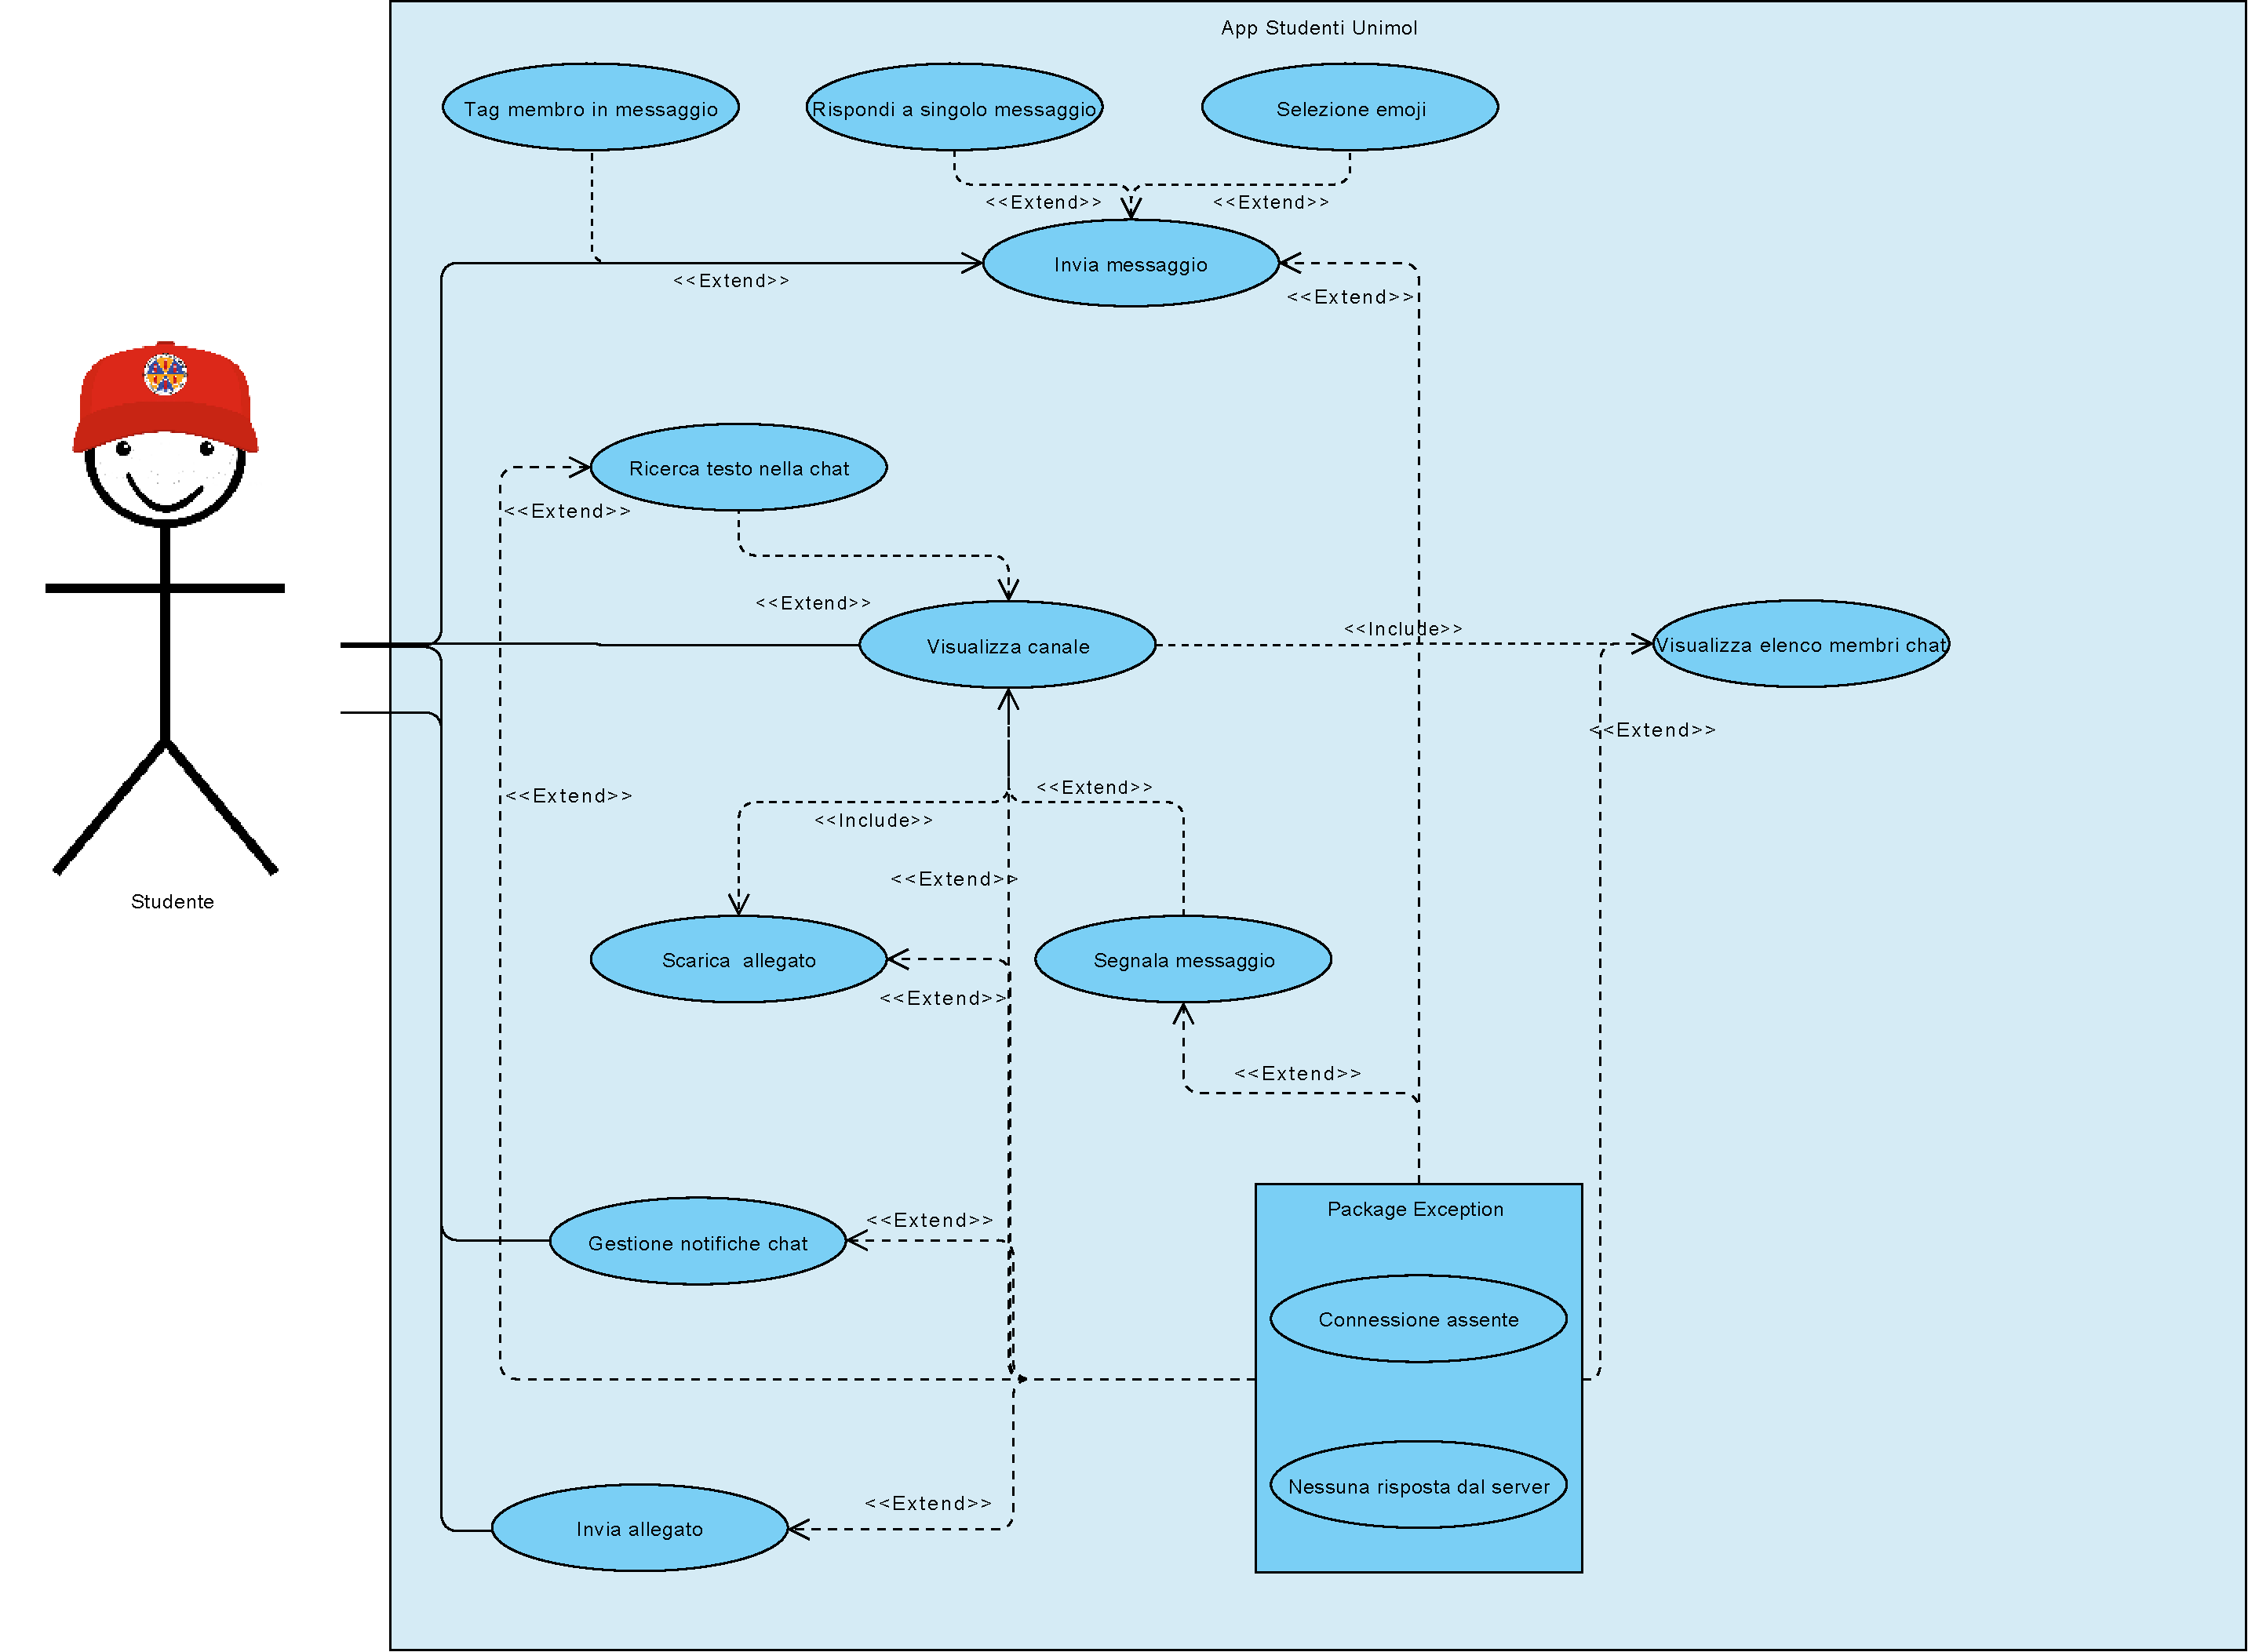
\includegraphics[height=3in]{imgs/gruppo6/use_case_diagrams/ucd1_chat_studenti.pdf}
	\caption{UCD1 - Chat Studenti}
	\label{fig:ucd1-stud}
\end{figure}

\begin{figure}
	\centering
	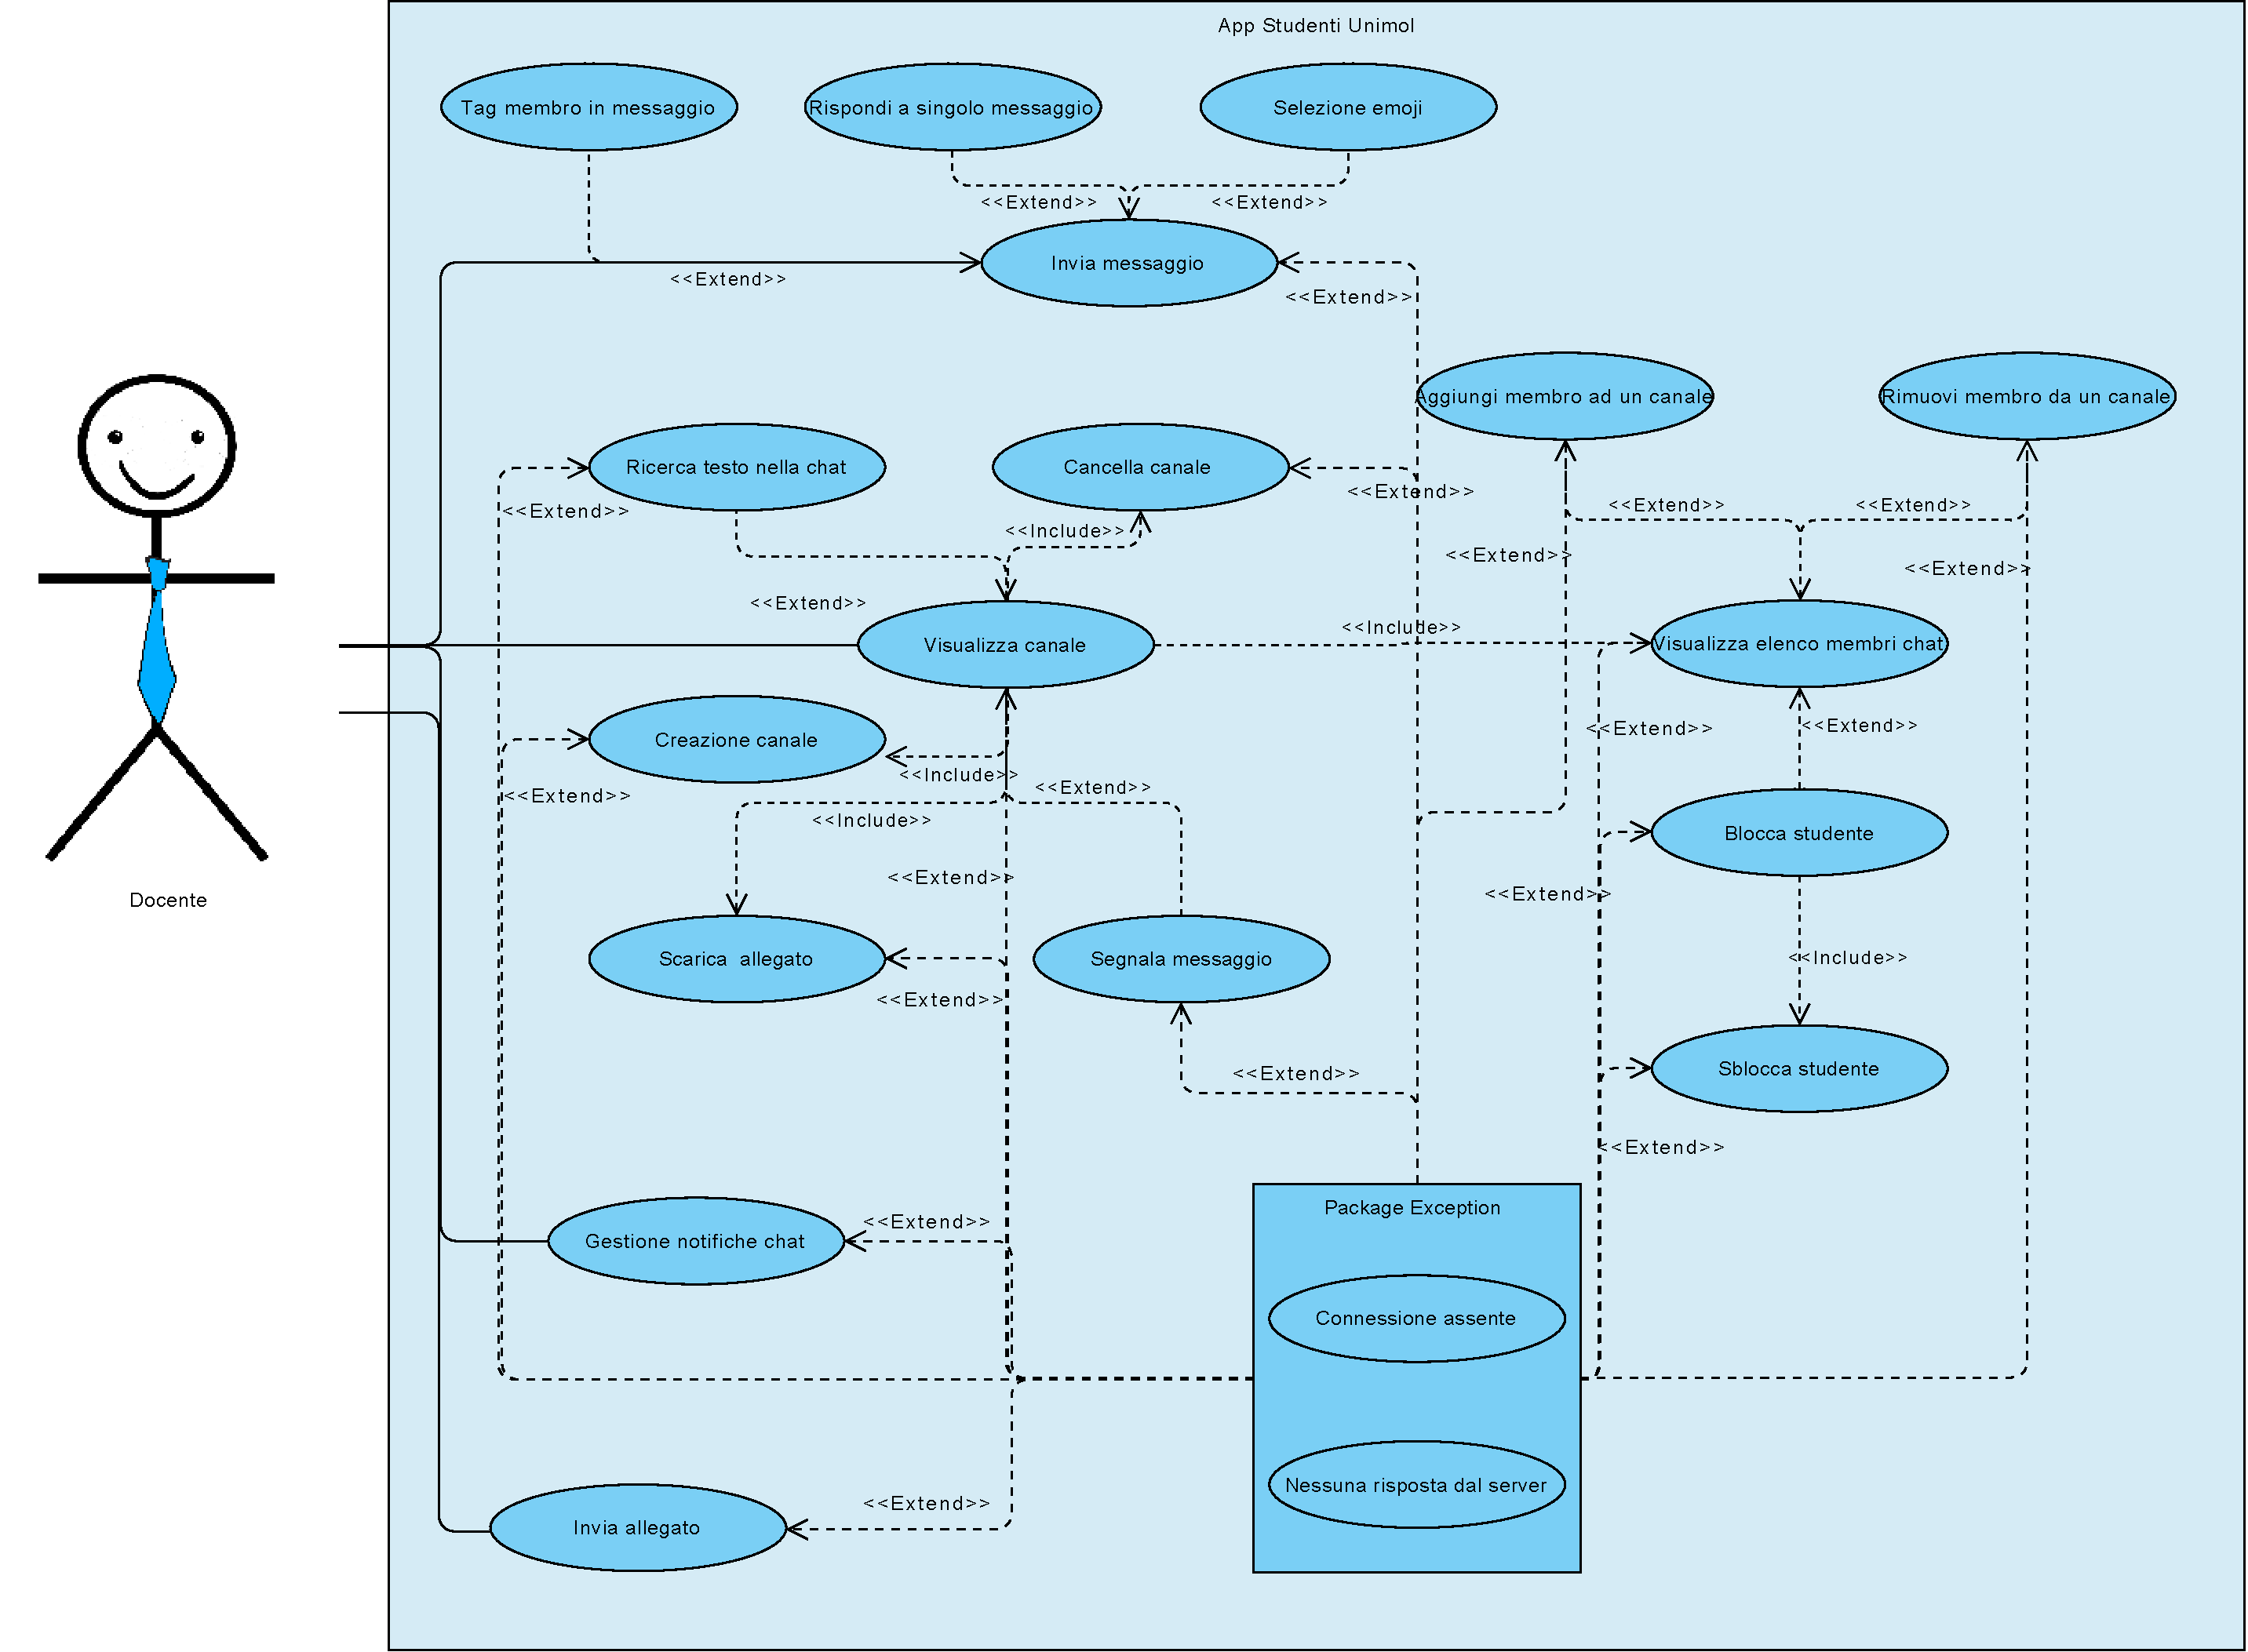
\includegraphics[height=3in]{imgs/gruppo6/use_case_diagrams/ucd2_chat_docenti.pdf}
	\caption{UCD2 - Chat Docenti}
	\label{fig:ucd2-doc}
\end{figure}

\begin{figure}
	\centering
	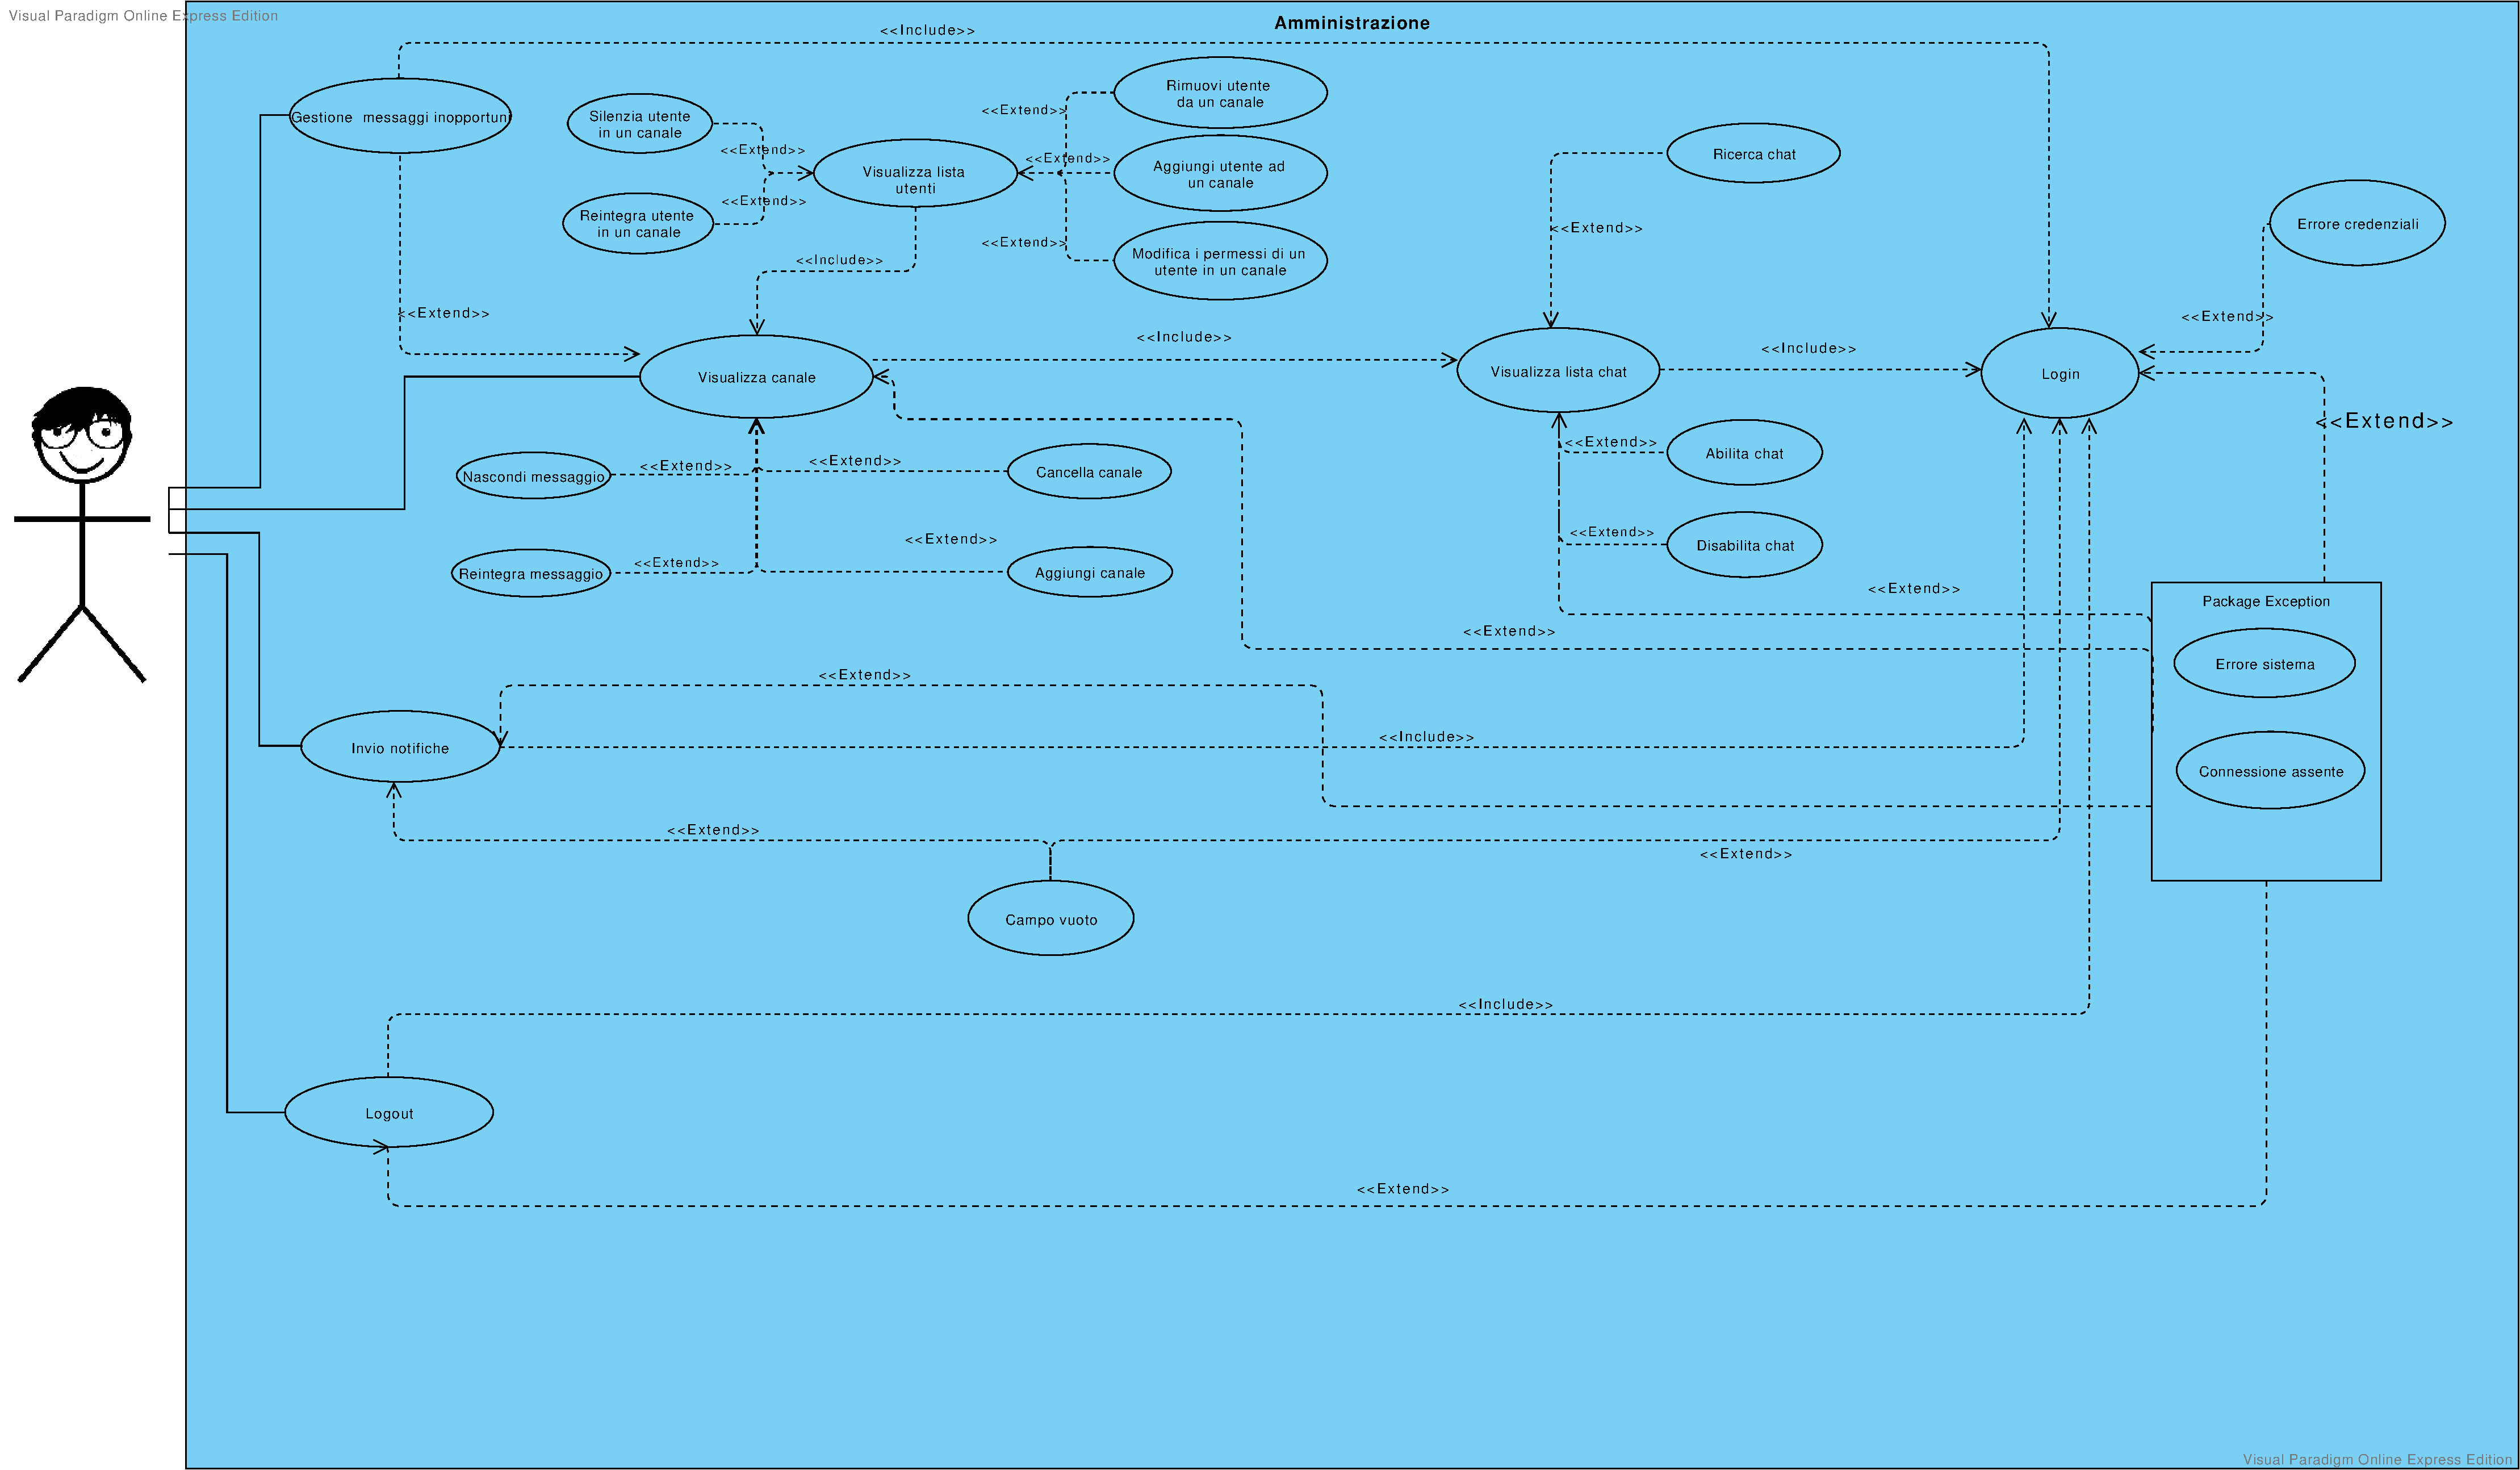
\includegraphics[height=3in]{imgs/gruppo6/use_case_diagrams/ucd3_pannello.pdf}
	\caption{UCD3 - Pannello di amministrazione}
	\label{fig:ucd3-amm}
\end{figure}

\clearpage
\subsection{Funzionalità rubrica}
\begin{figure}[H]
	\centering
	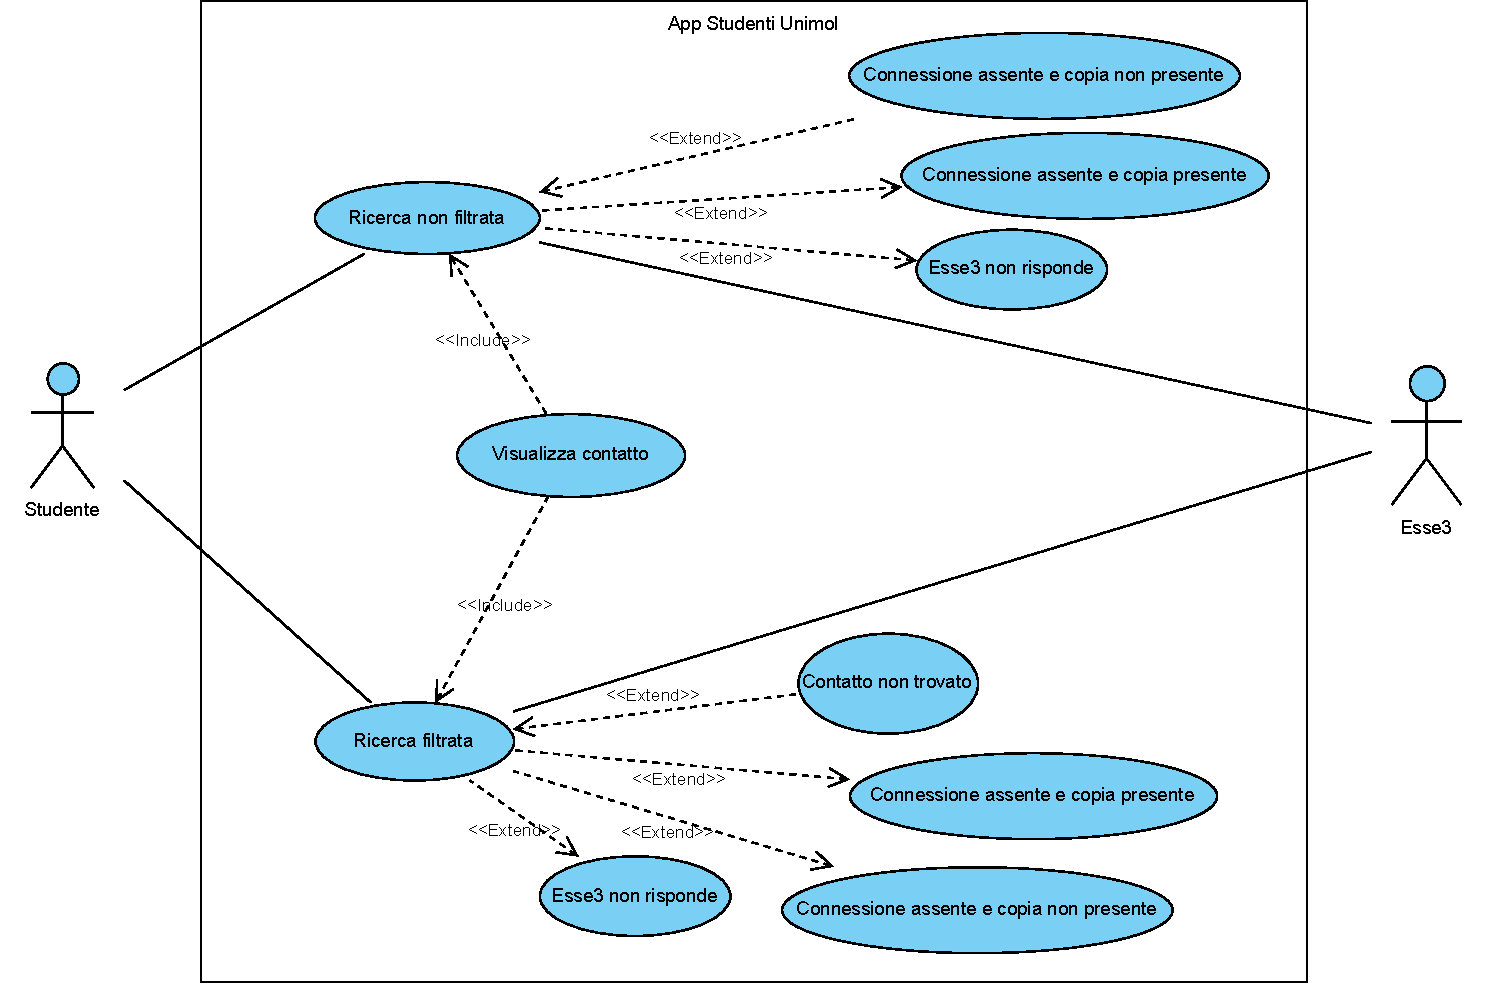
\includegraphics[height=3in]{imgs/gruppo5/Diagram1.pdf}
	\caption{UCD - Rubrica}
	\label{fig:ucd-rubrica}
\end{figure}

\clearpage
\subsection{Funzionalità previsione media}
\begin{figure}[H]
	\centering
	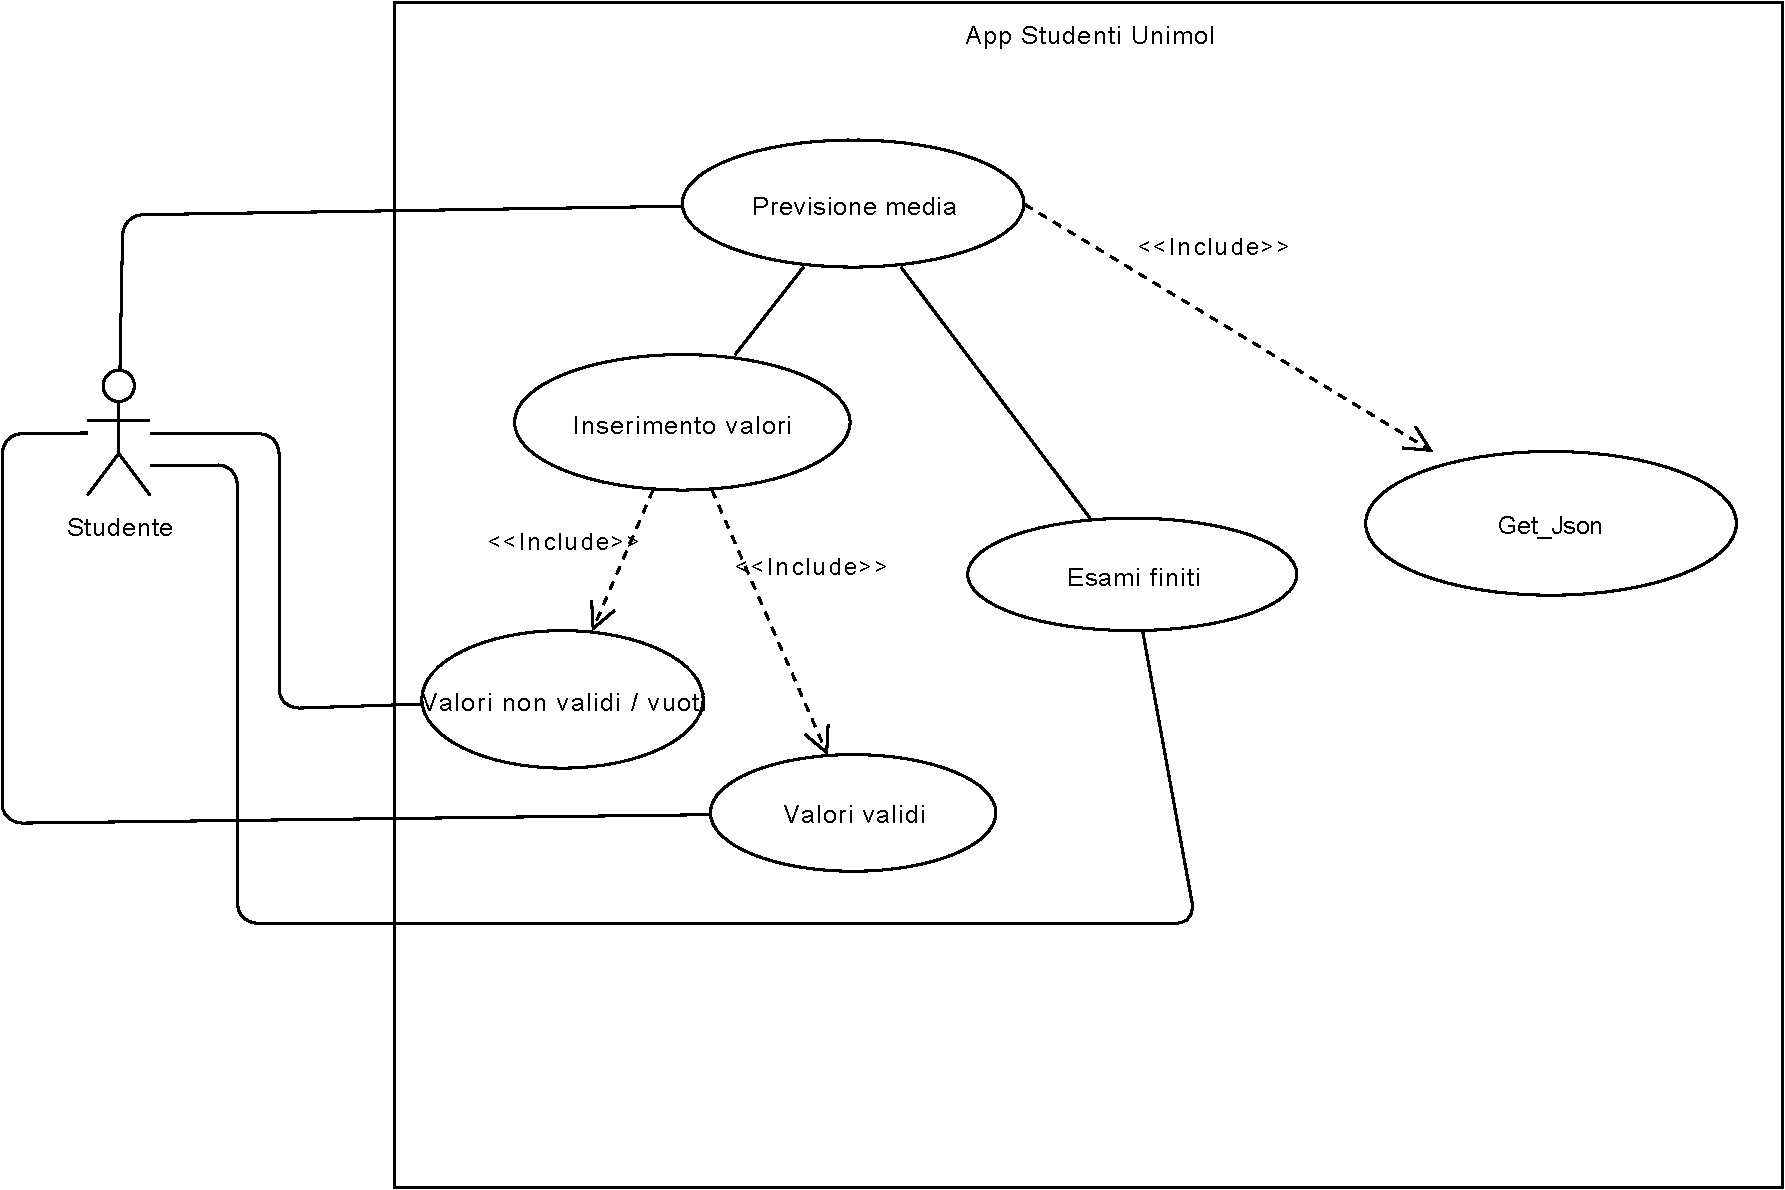
\includegraphics[height=4in]{imgs/gruppo3/caso-duso-media.pdf}
	\caption{UCD - Previsione Media}
	\label{fig:prova}
\end{figure}

\newpage
\section{Diagramma di sequenza}

\subsection{Funzionalità chat}

\subsubsection{Chat studenti}
\begin{figure}[!h]
	\centering
	%%% cambiare height=3in,width=5in -> width=0.9\textwidth
	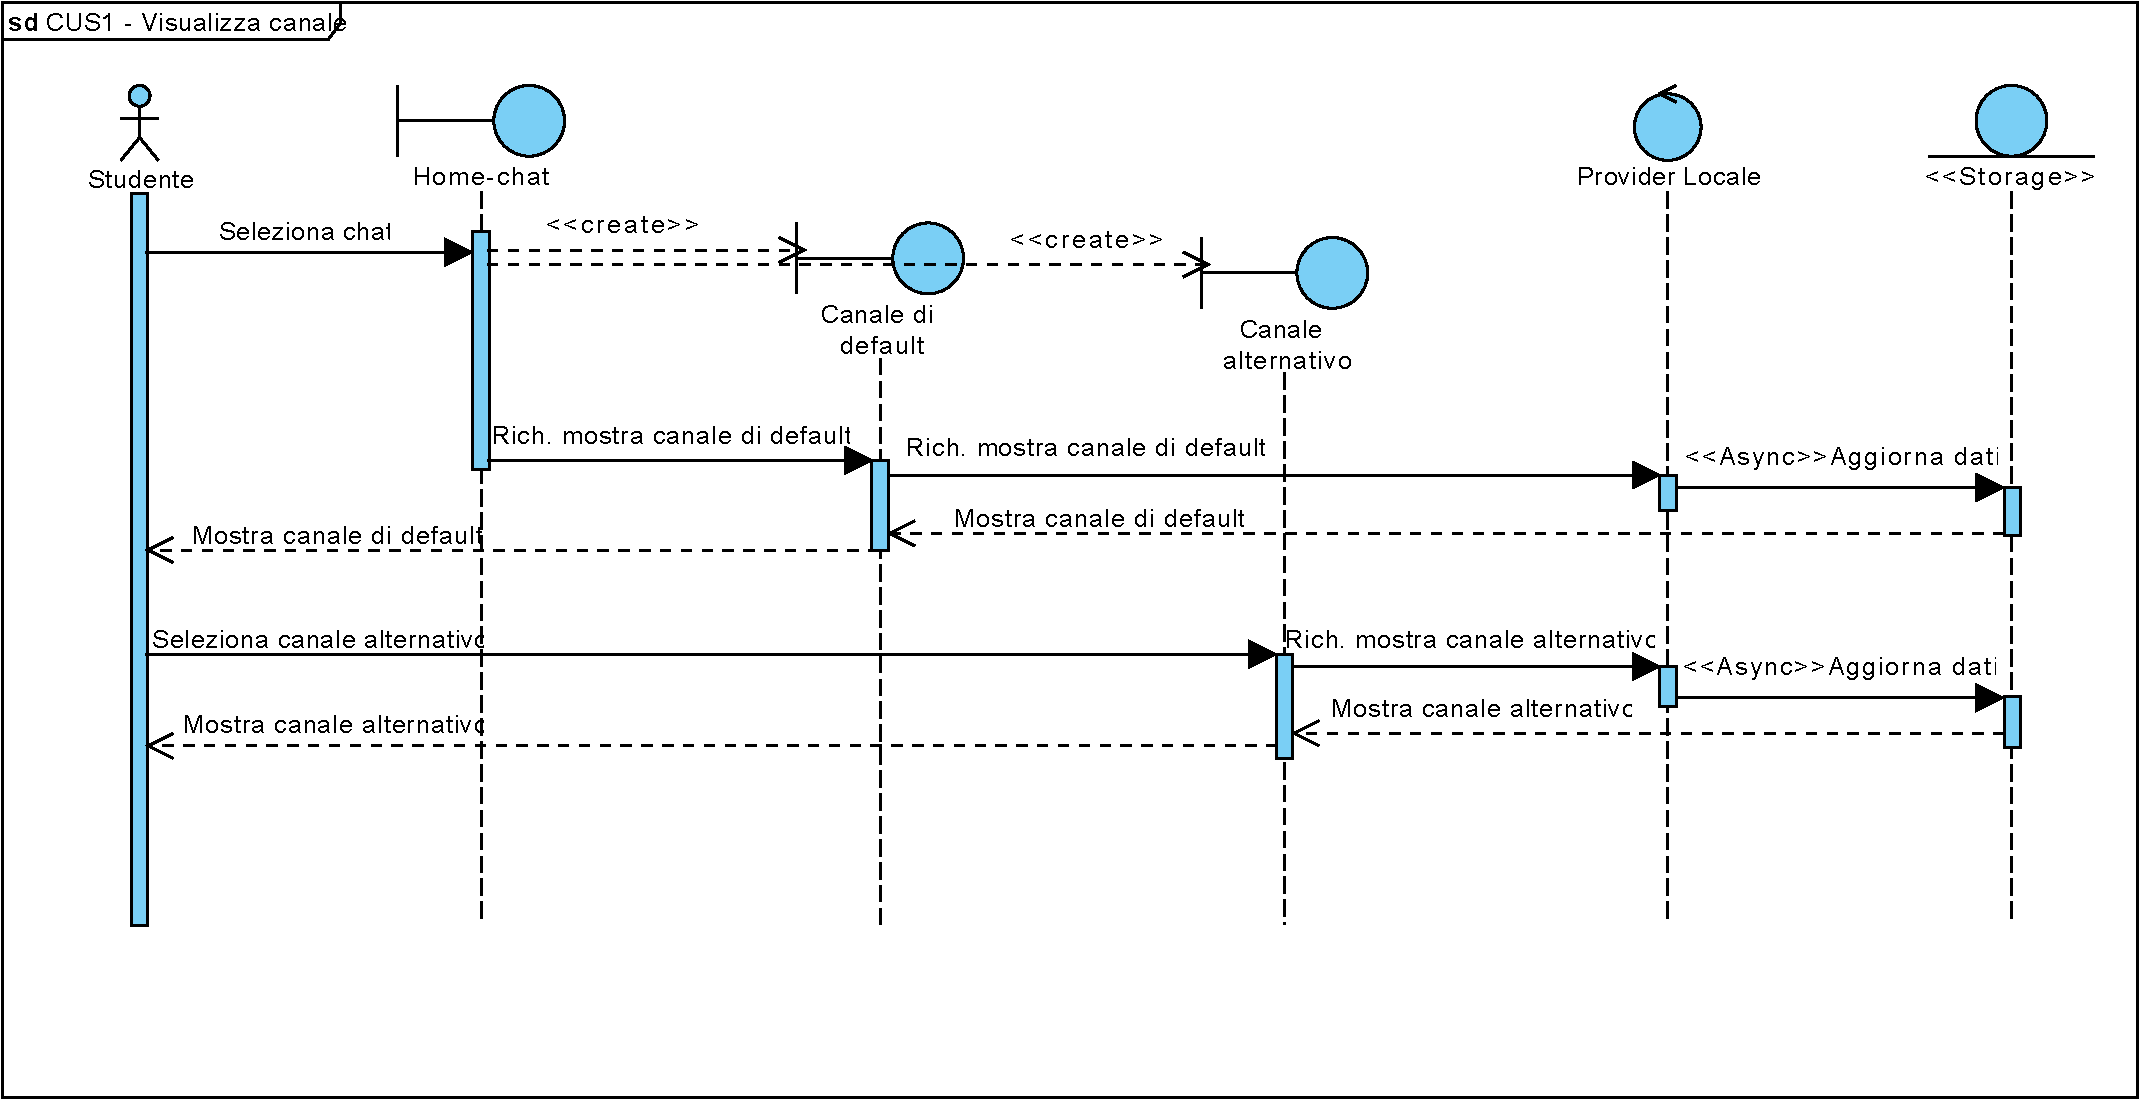
\includegraphics[width=0.9\textwidth]{imgs/gruppo6/sequence/CUS1_visualizza_canale.pdf}
	\caption{CUS1 - Visualizza canale}
	%%% \label{fig:seq-cus1}
	\label{fig:seq-cus1}
\end{figure}

\begin{figure}
	\centering
	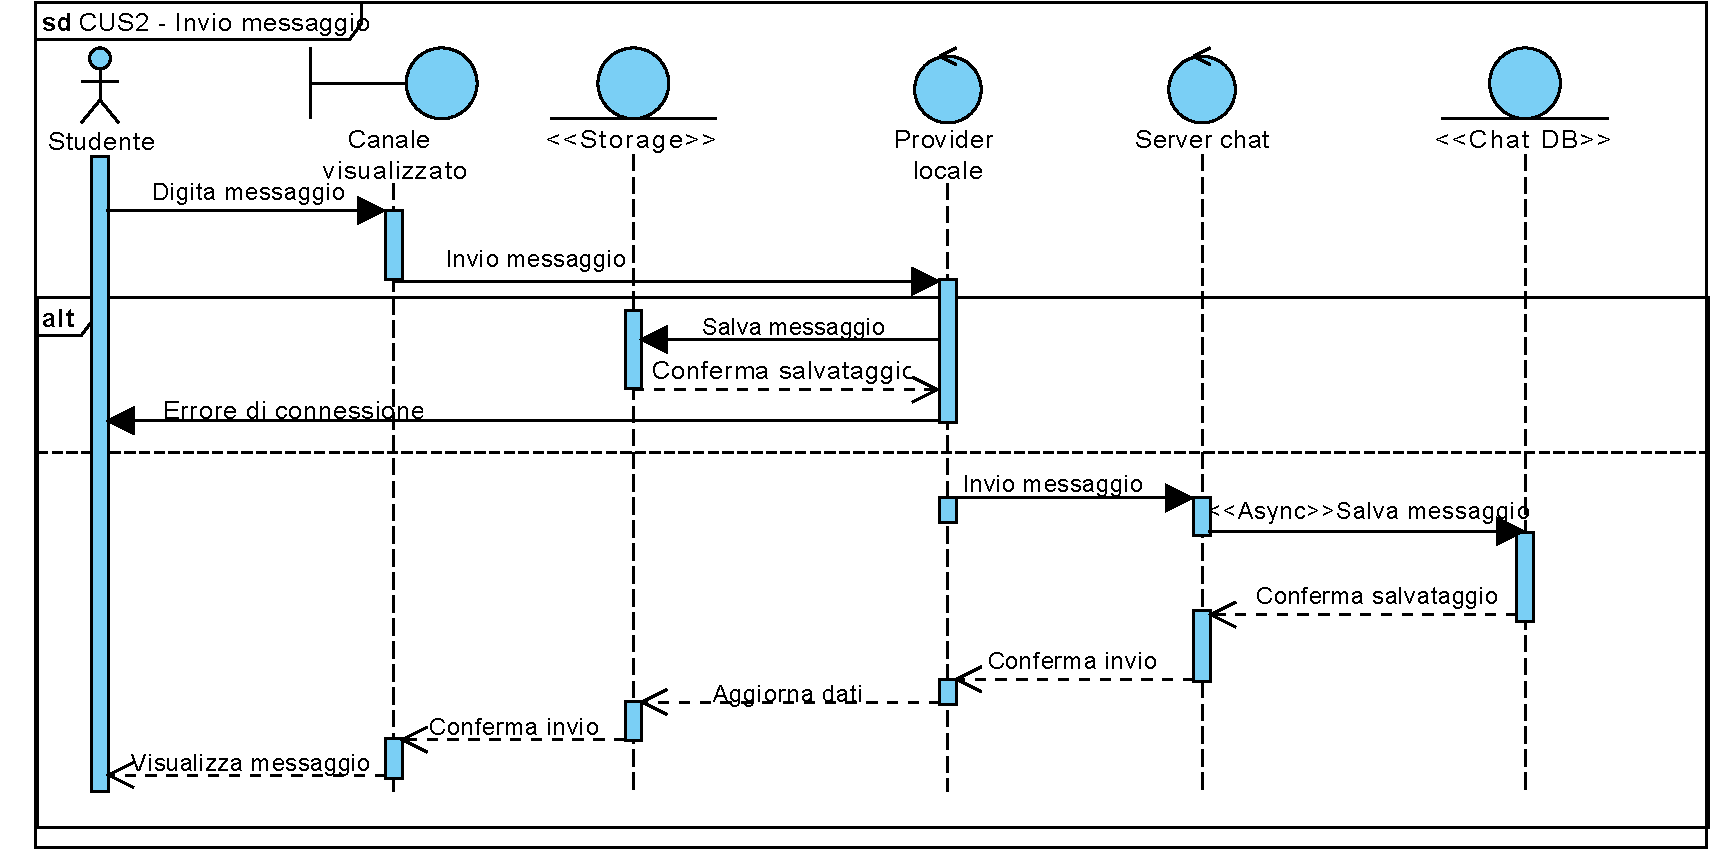
\includegraphics[width=0.9\textwidth]{imgs/gruppo6/sequence/CUS2_invio_messaggio.pdf}
	\caption{CUS2 - Invio messaggio}
	\label{fig:seq-cus2}
\end{figure}

\begin{figure}
	\centering
	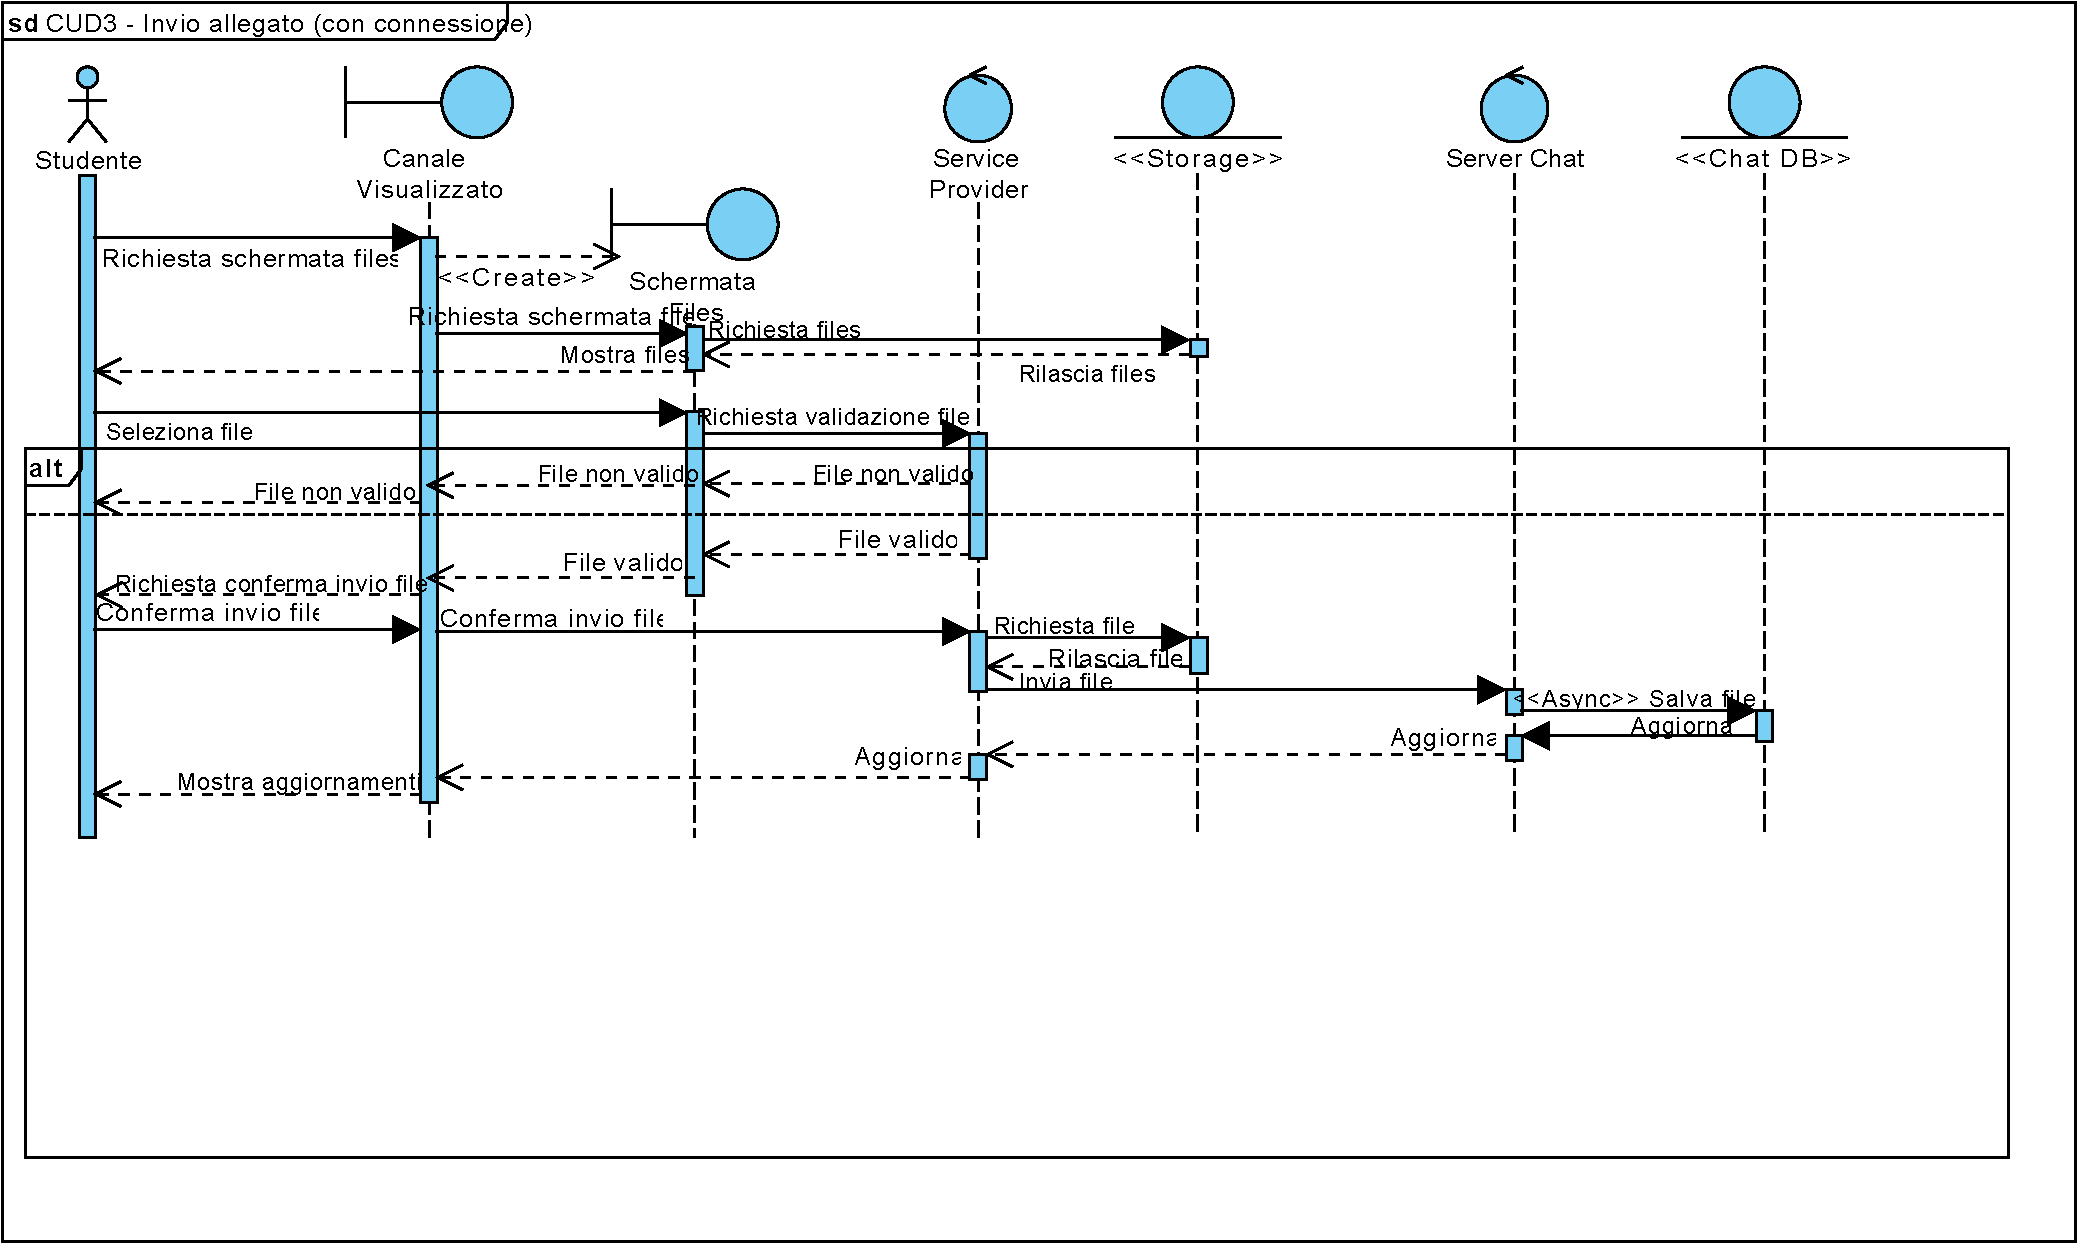
\includegraphics[width=0.9\textwidth]{imgs/gruppo6/sequence/CUS3_invio_allegato.pdf}
	\caption{CUS3 - Invio allegato}
	\label{fig:seq-cus3}
\end{figure}

\begin{figure}
	\centering
	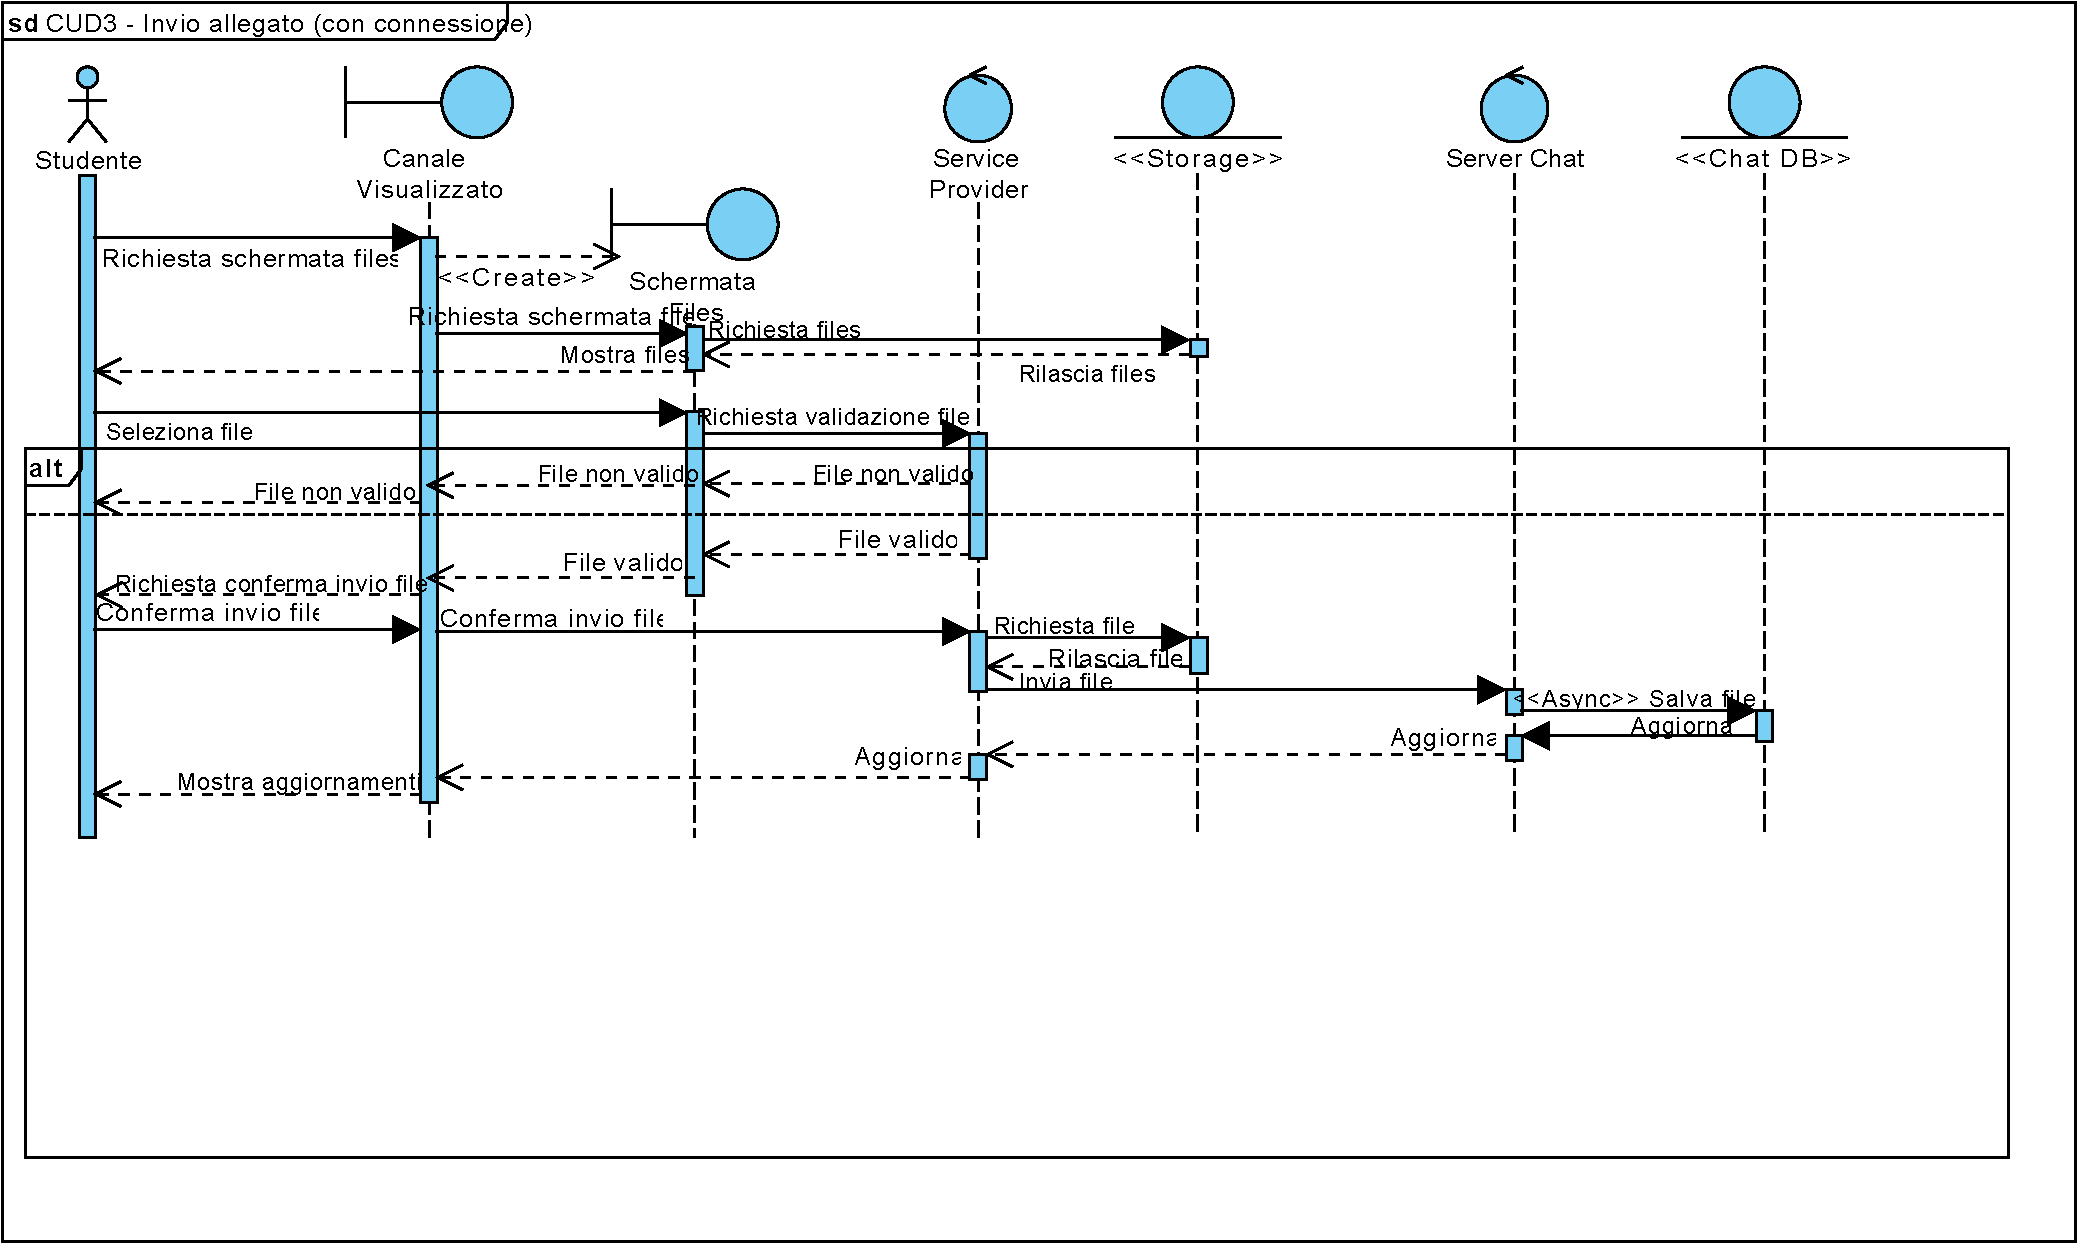
\includegraphics[width=0.9\textwidth]{imgs/gruppo6/sequence/CUS3_invio_allegato.pdf}
	\caption{CUS3.1 - Invio allegato}
	\label{fig:seq-cus3mod}
\end{figure}

\begin{figure}
	\centering
	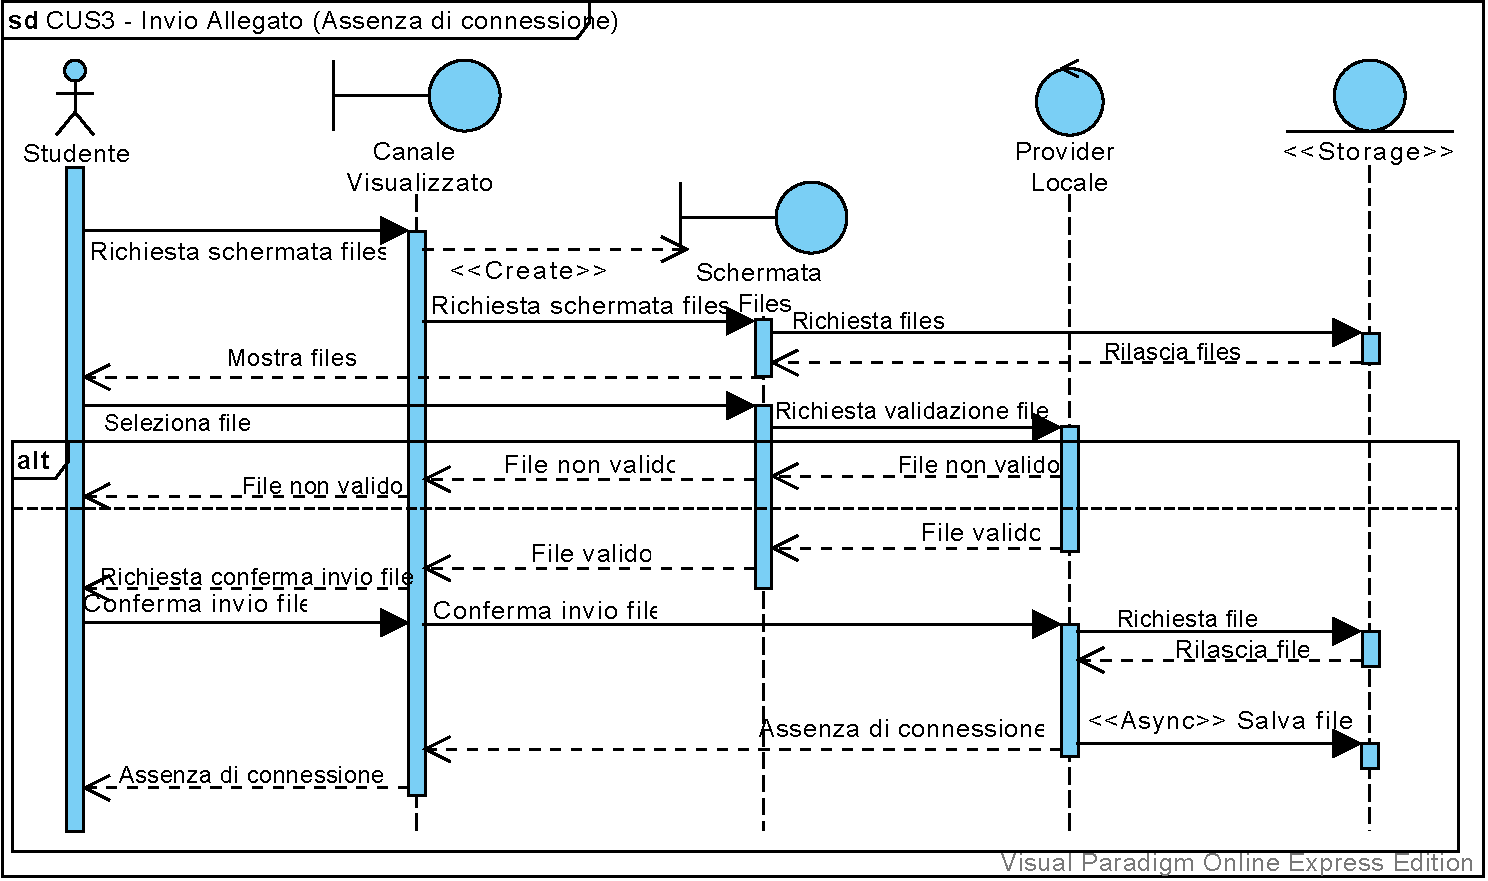
\includegraphics[width=0.9\textwidth]{imgs/gruppo6/sequence/CUS3_invio_allegato_no_connessione.pdf}
	\caption{CUS3.2 - Invio allegato in assenza di connessione}
	\label{fig:seq-cus3mod1}
\end{figure}

\begin{figure}
	\centering
	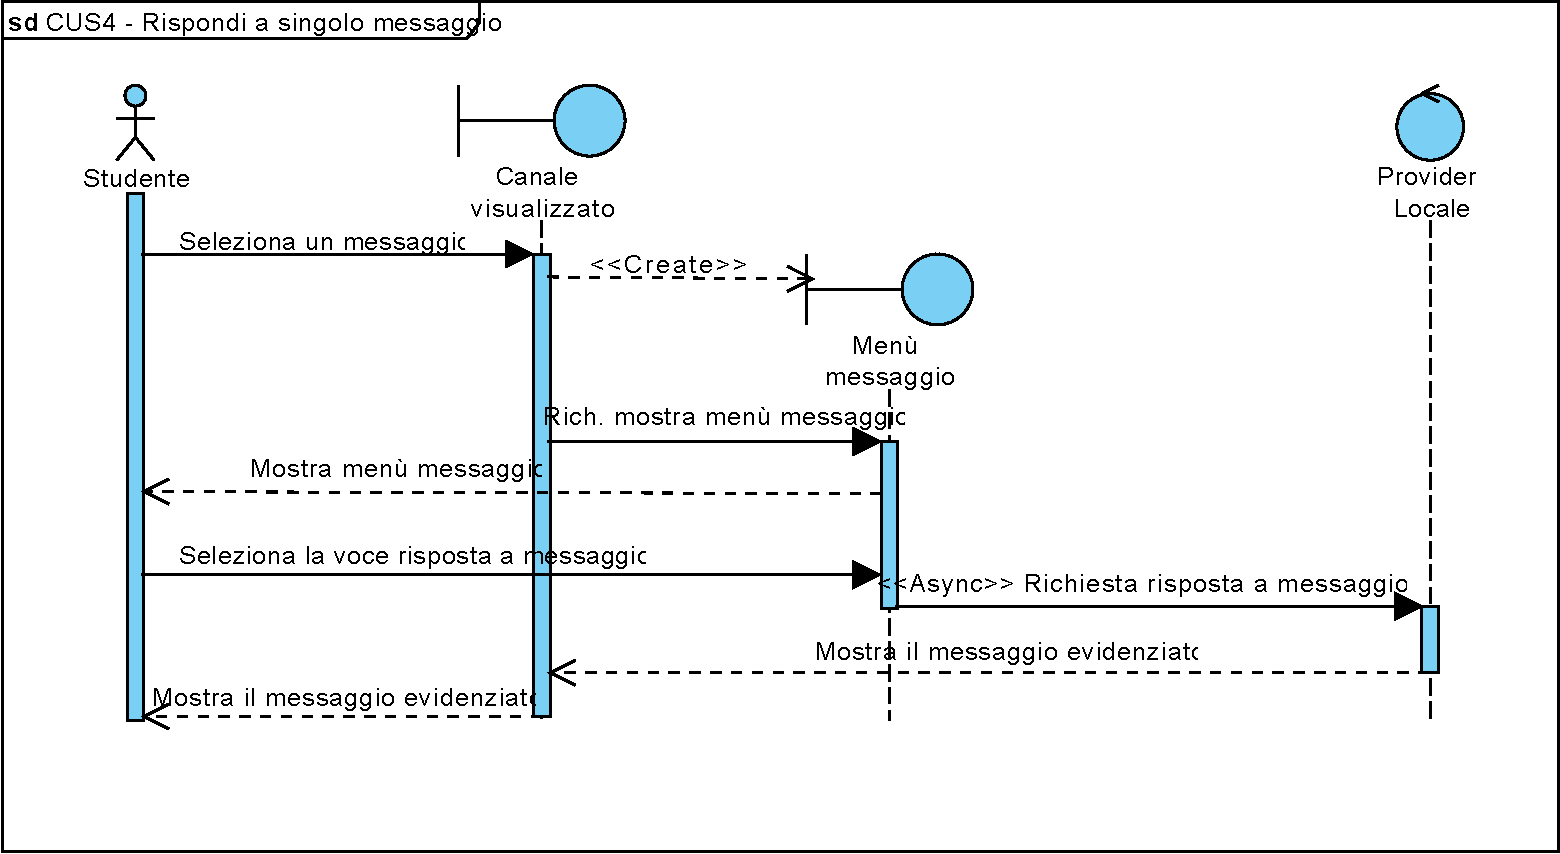
\includegraphics[width=0.9\textwidth]{imgs/gruppo6/sequence/CUS4_rispondi_a_singolo_messaggio.pdf}
	\caption{CUS4 - Rispondi a singolo messaggio}
	\label{fig:seq-cus4}
\end{figure}

\begin{figure}
	\centering
	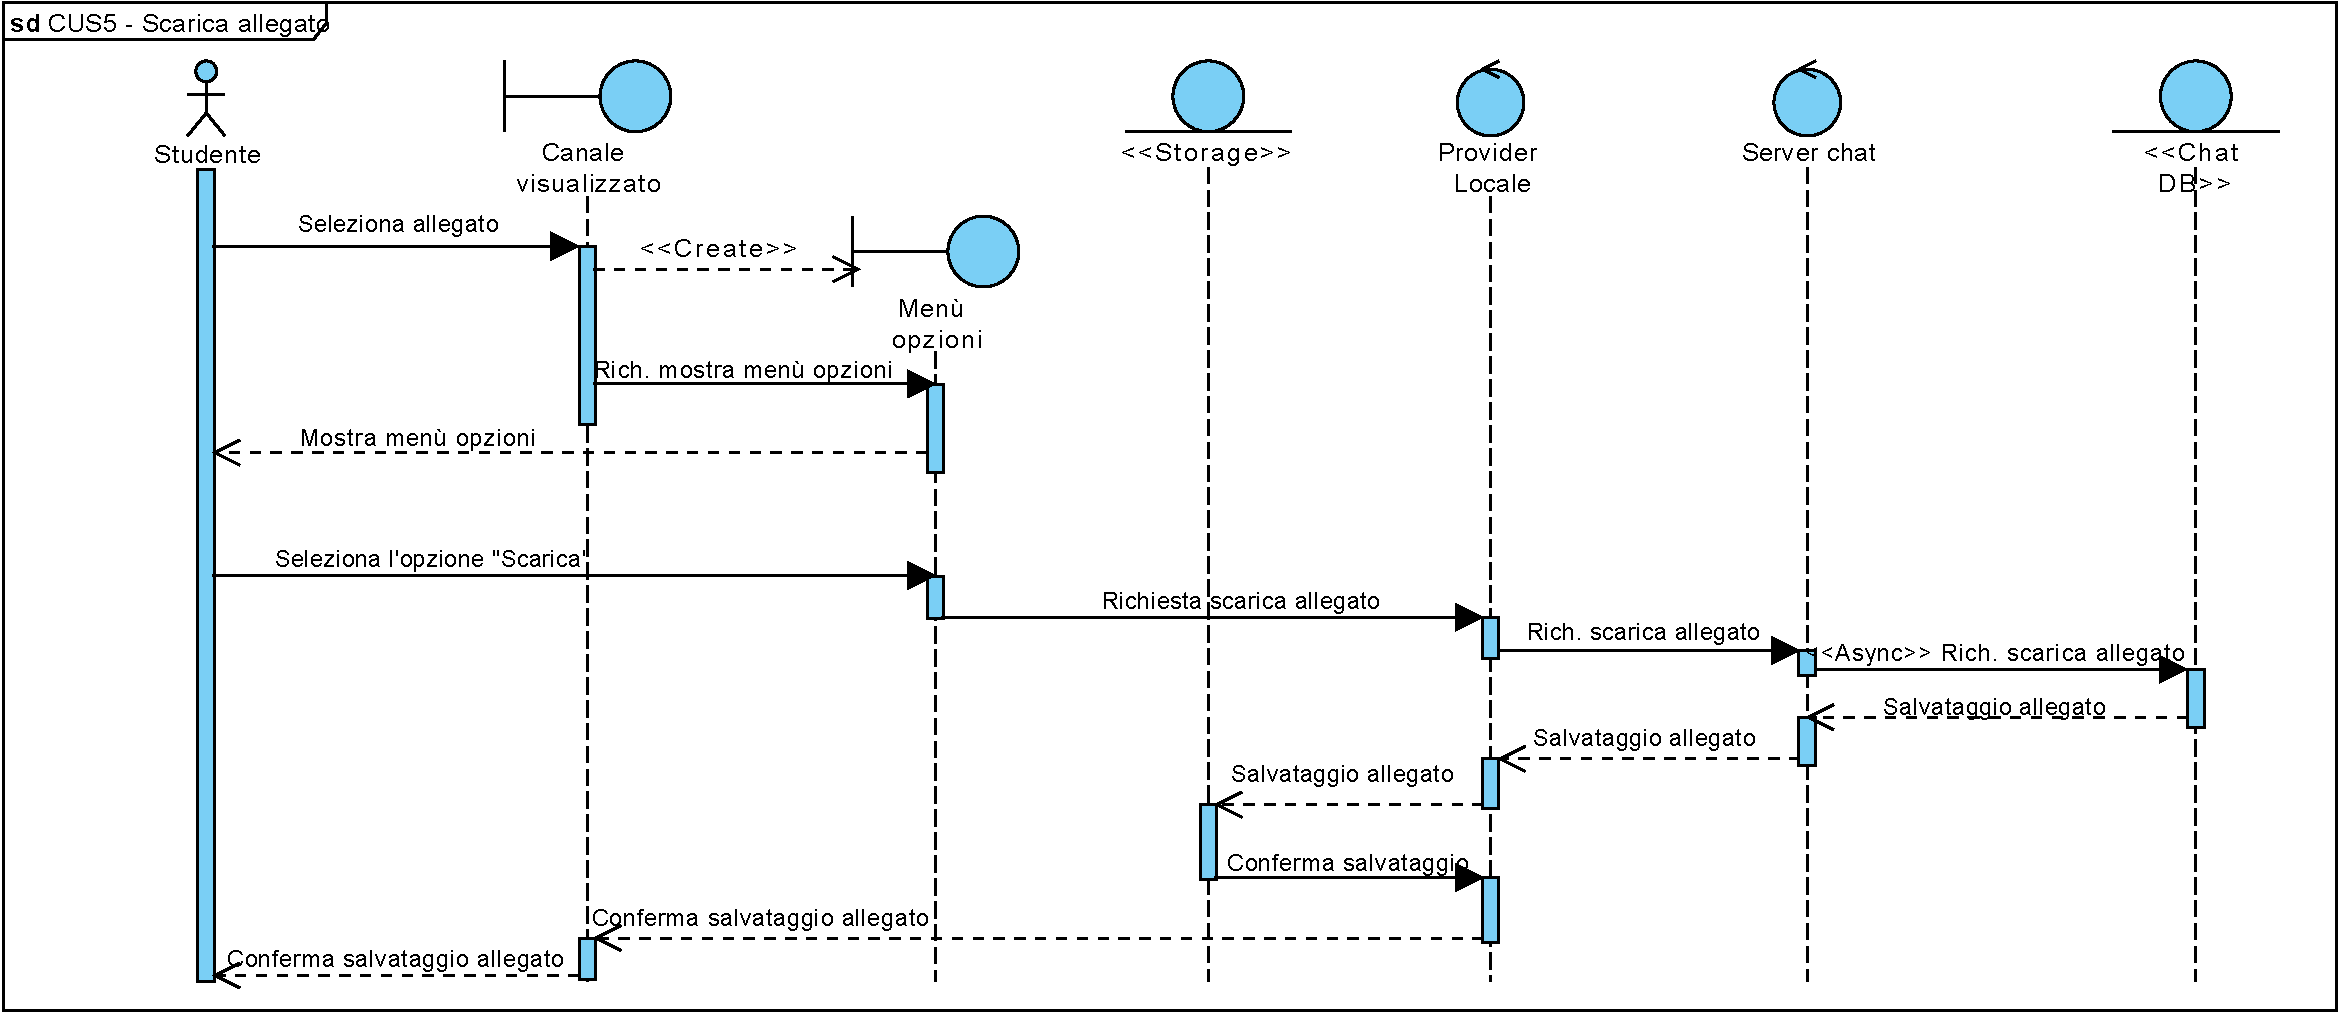
\includegraphics[width=0.9\textwidth]{imgs/gruppo6/sequence/CUS5_scarica_allegato.pdf}
	\caption{CUS5 - Scarica allegato}
	\label{fig:seq-cus5}
\end{figure}

\begin{figure}
	\centering
	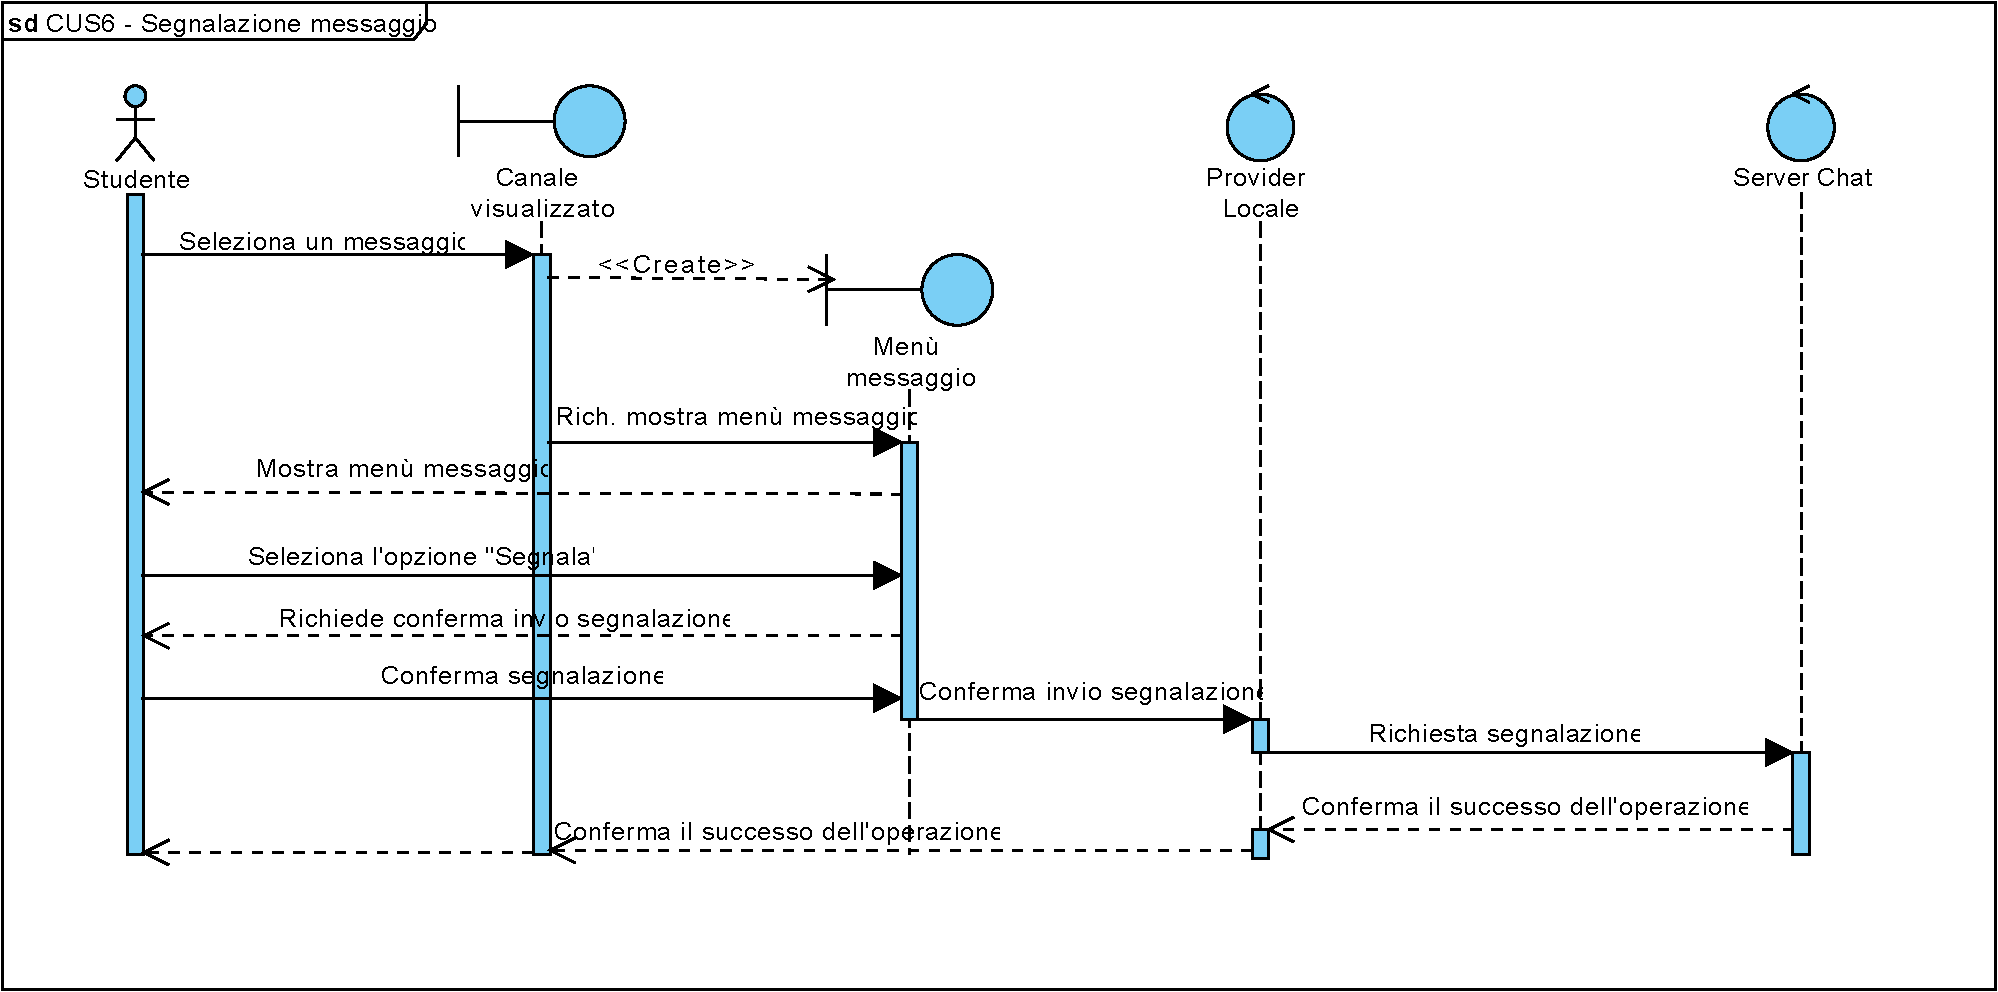
\includegraphics[width=0.9\textwidth]{imgs/gruppo6/sequence/CUS6_segnalazione_messaggio.pdf}
	\caption{CUS6 - Segnalazione messaggio}
	\label{fig:seq-cus6}
\end{figure}

\begin{figure}
	\centering
	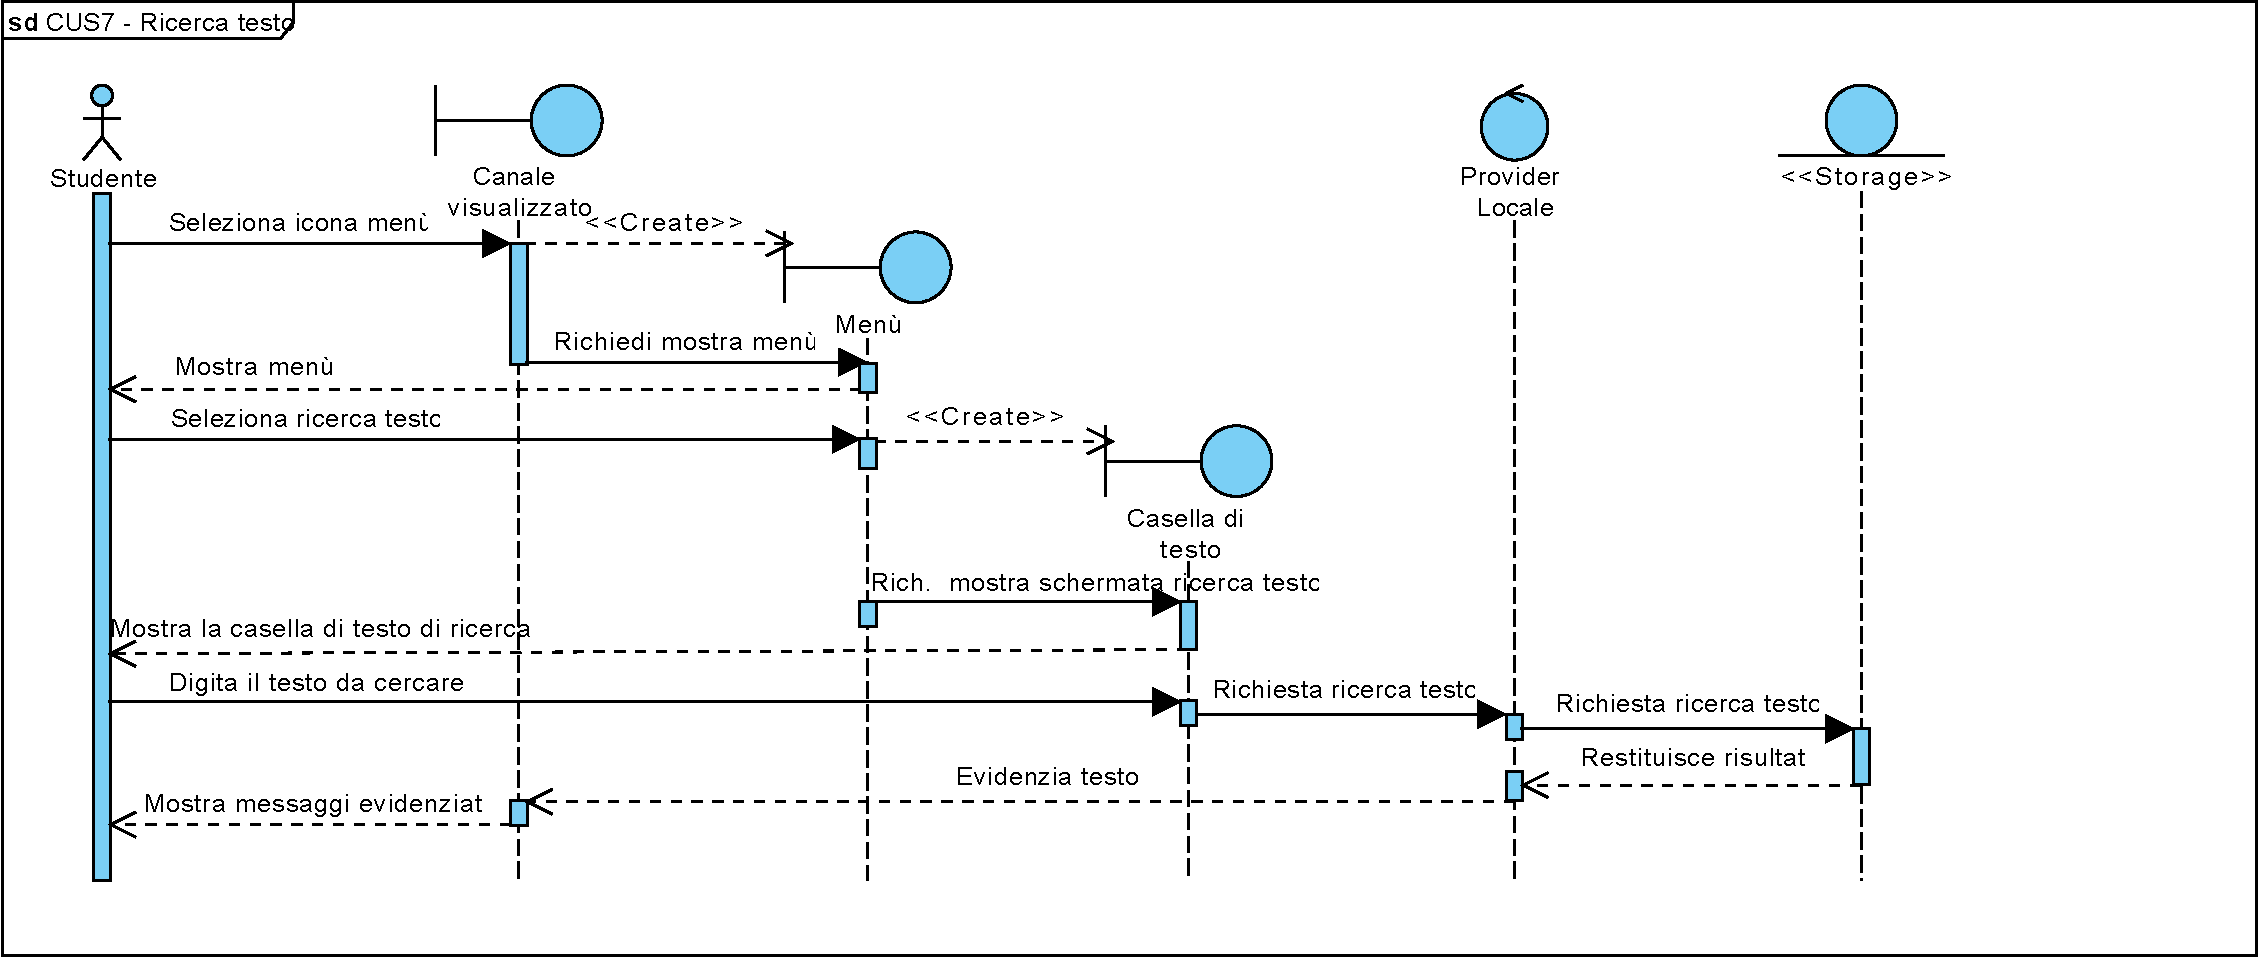
\includegraphics[width=0.9\textwidth]{imgs/gruppo6/sequence/CUS7_ricerca_testo.pdf}
	\caption{CUS7 - Ricerca testo}
	\label{fig:seq-cus7}
\end{figure}

\begin{figure}
	\centering
	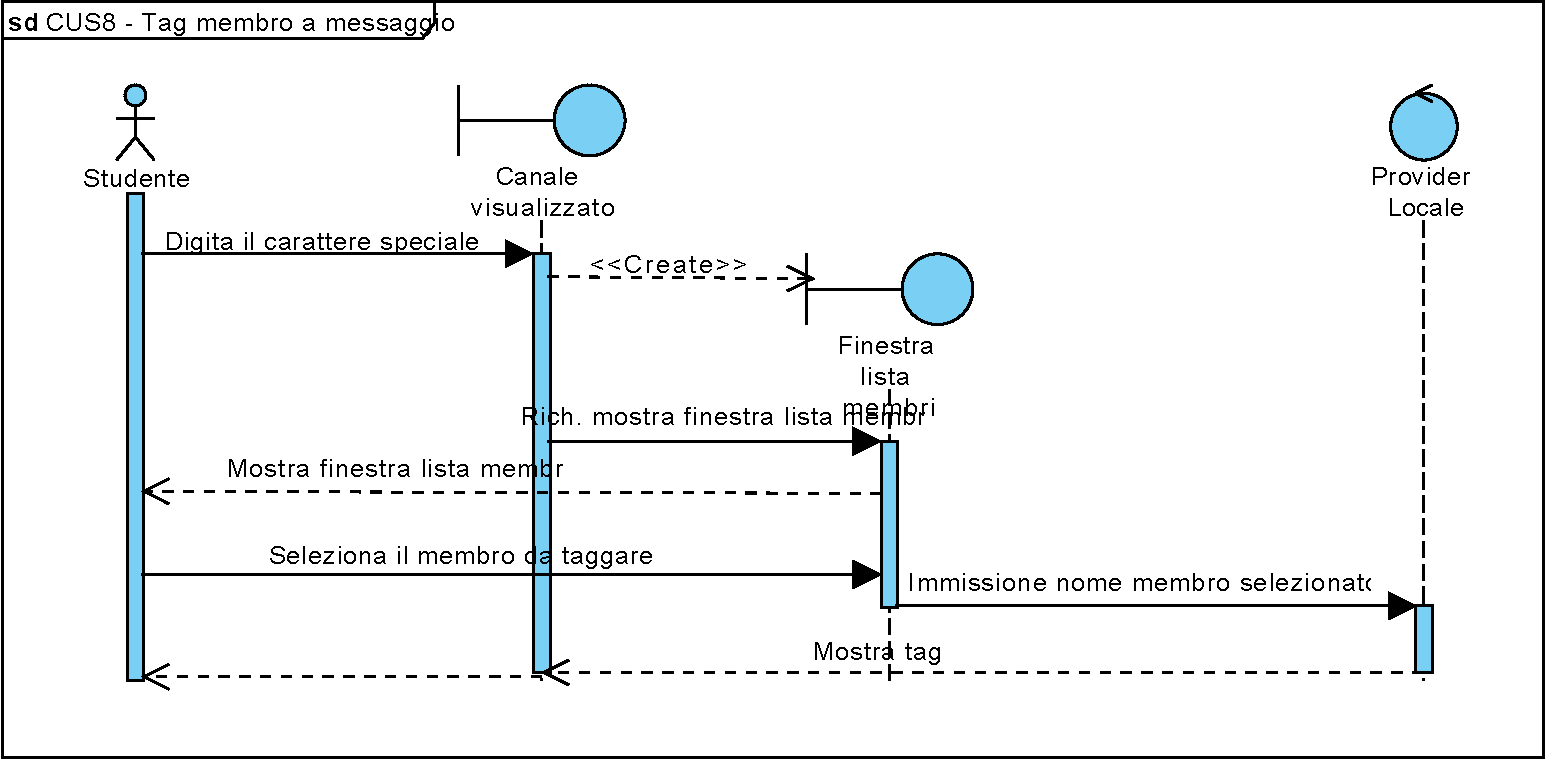
\includegraphics[width=0.9\textwidth]{imgs/gruppo6/sequence/CUS8_tag_membro_a_messaggio.pdf}
	\caption{CUS8 - Tag membro a messaggio}
	\label{fig:seq-cus8}
\end{figure}

\begin{figure}
	\centering
	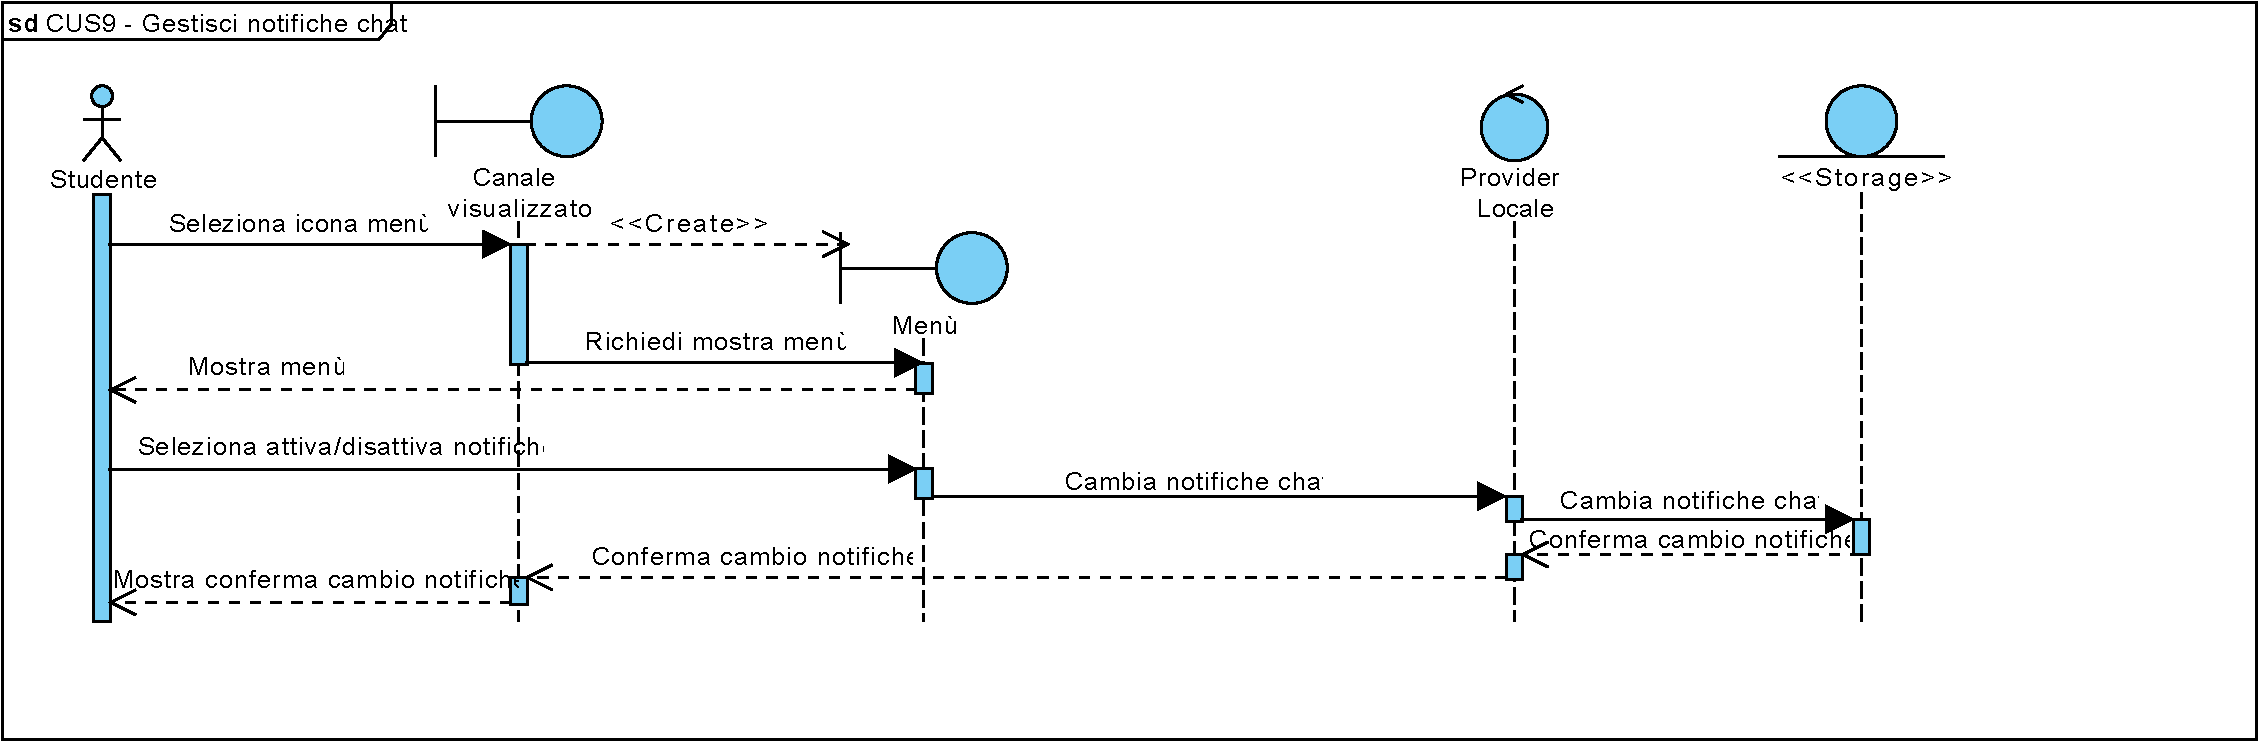
\includegraphics[width=0.9\textwidth]{imgs/gruppo6/sequence/CUS9_gestisci_notifiche_chat.pdf}
	\caption{CUS9 - Gestisci notifiche chat}
	\label{fig:seq-cus9}
\end{figure}

\begin{figure}
	\centering
	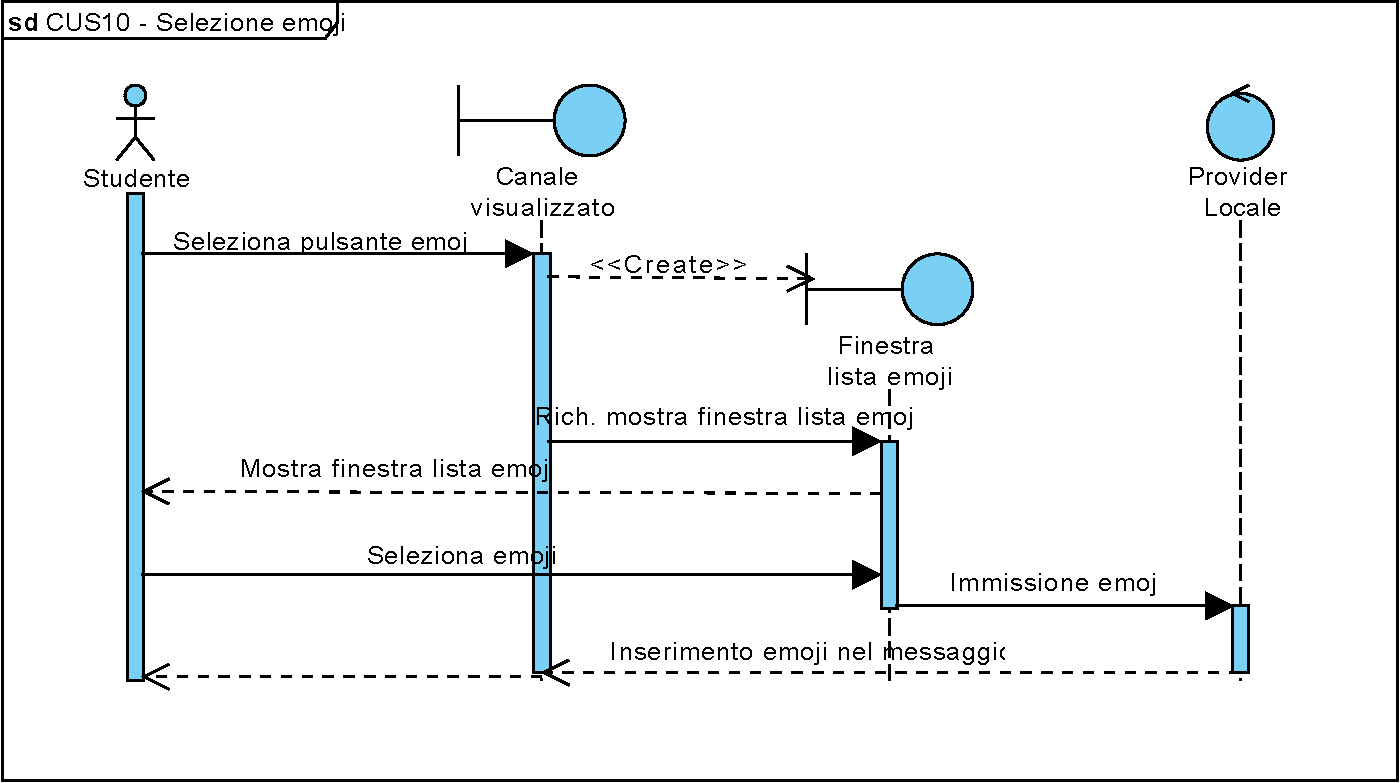
\includegraphics[width=0.9\textwidth]{imgs/gruppo6/sequence/CUS10_selezione_emoji.pdf}
	\caption{CUS10 - Seleziona emoji}
	\label{fig:seq-cus10}
\end{figure}

\begin{figure}
	\centering
	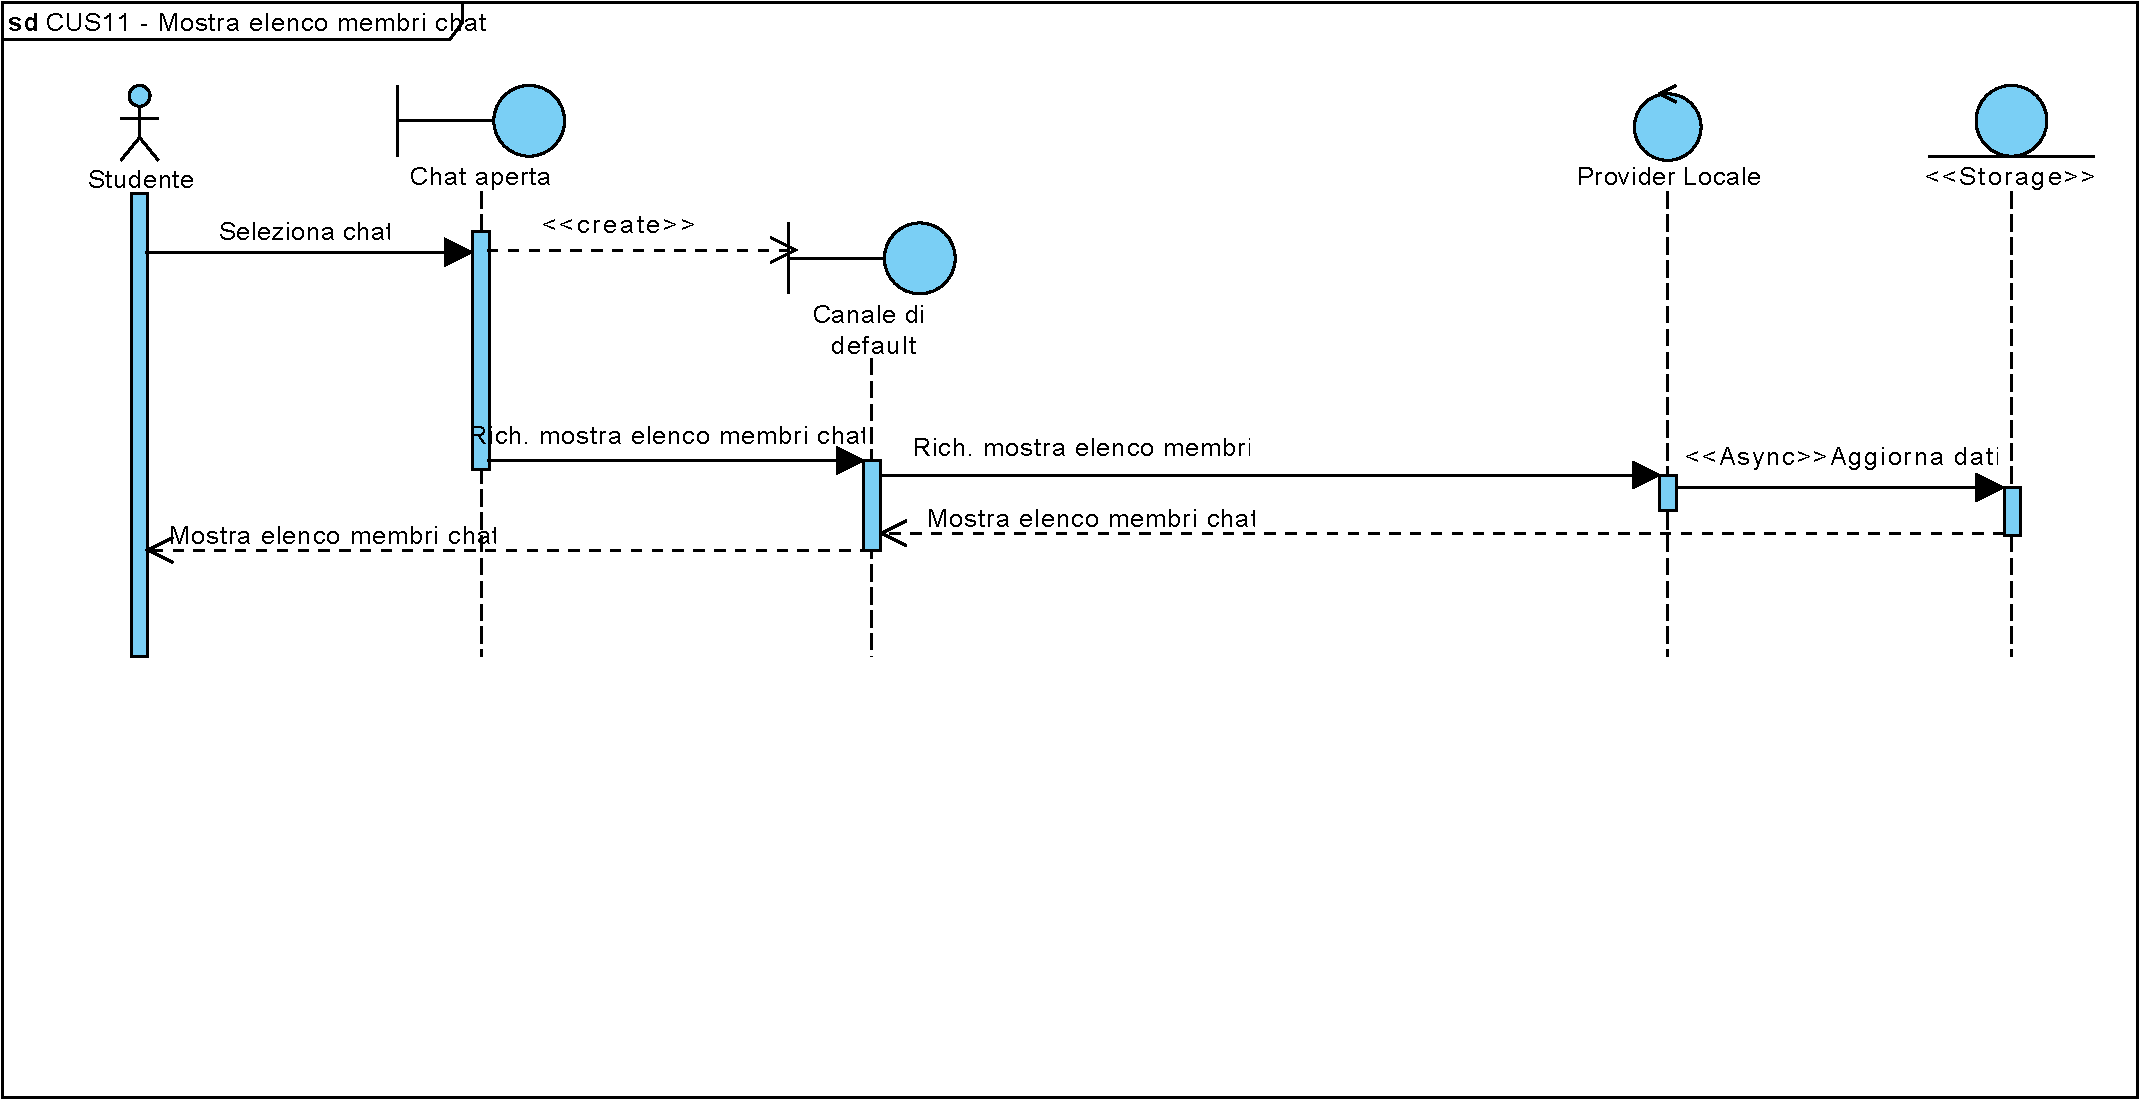
\includegraphics[width=0.9\textwidth]{imgs/gruppo6/sequence/CUS11_visualizza_elenco_membri_chat.pdf}
	\caption{CUS11 - Visualizza elenco membri chat}
	\label{fig:seq-cus11}
\end{figure}

\pagebreak
\subsubsection{Chat docenti}
\begin{figure}[!h]
	\centering
	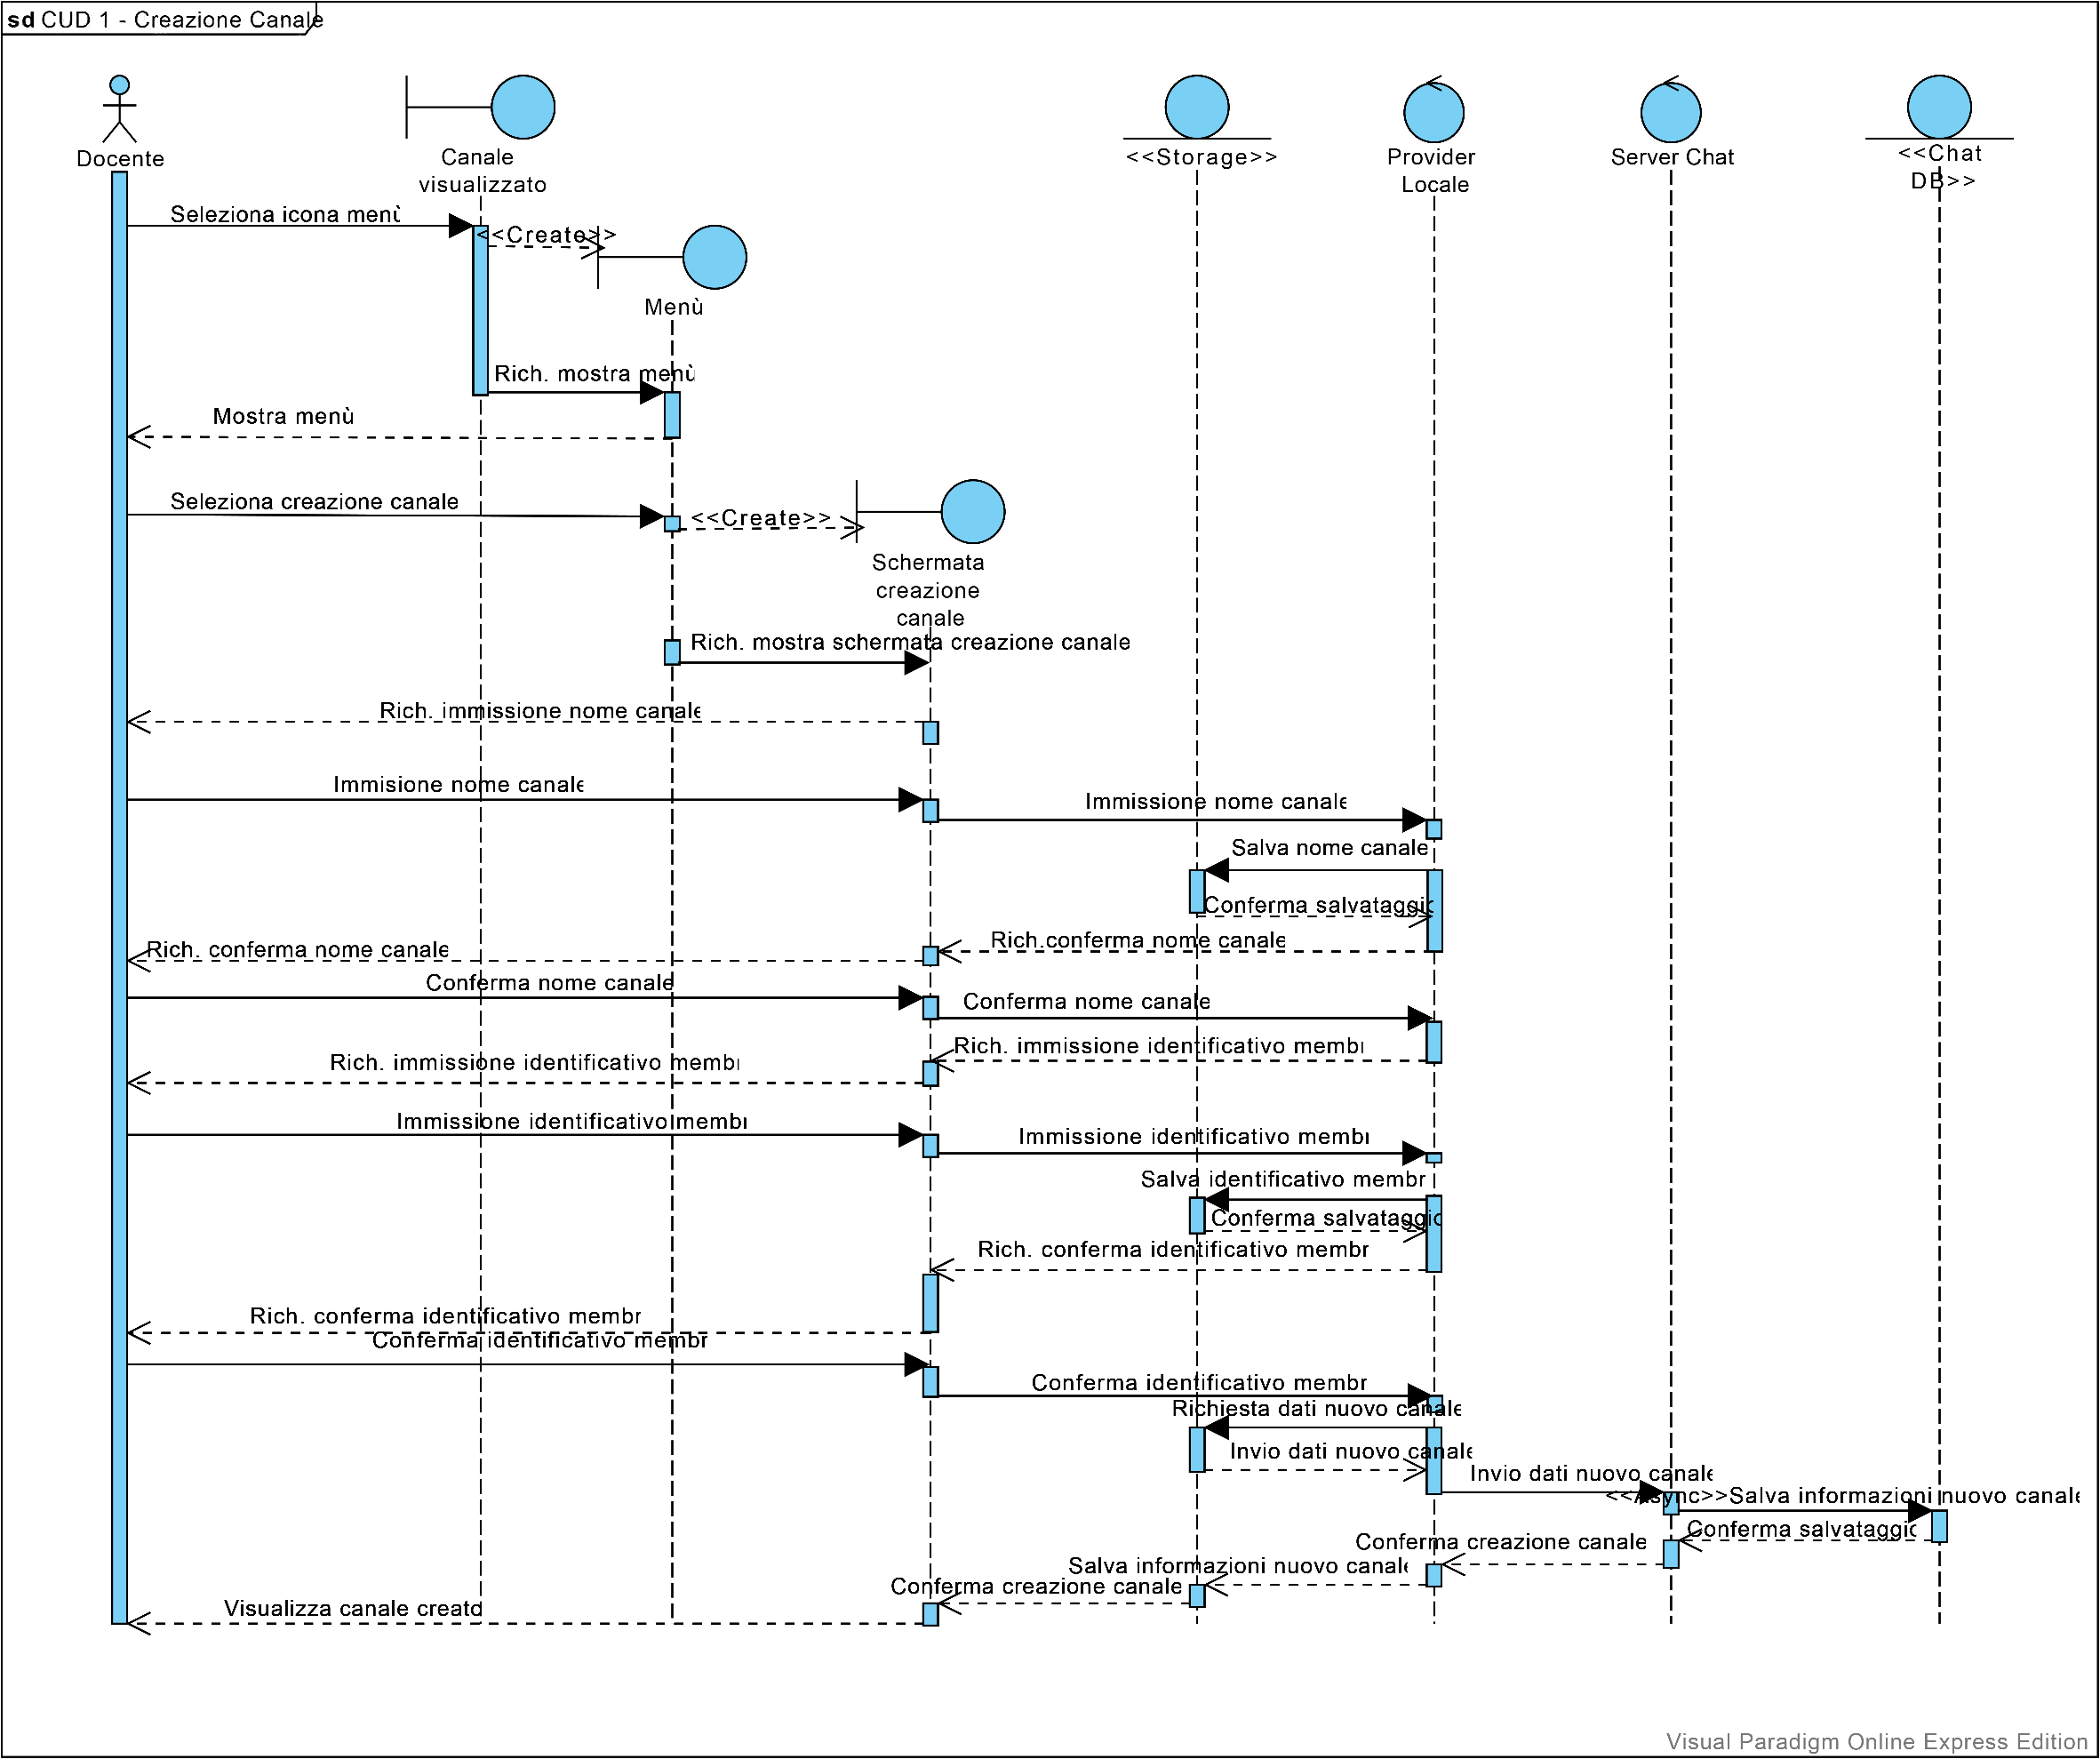
\includegraphics[width=0.9\textwidth]{imgs/gruppo6/sequence/CUD1_creazione_canale.pdf}
	\caption{CUD1 - Creazione canale}
	\label{fig:seq-cud1}
\end{figure}

\begin{figure}
	\centering
	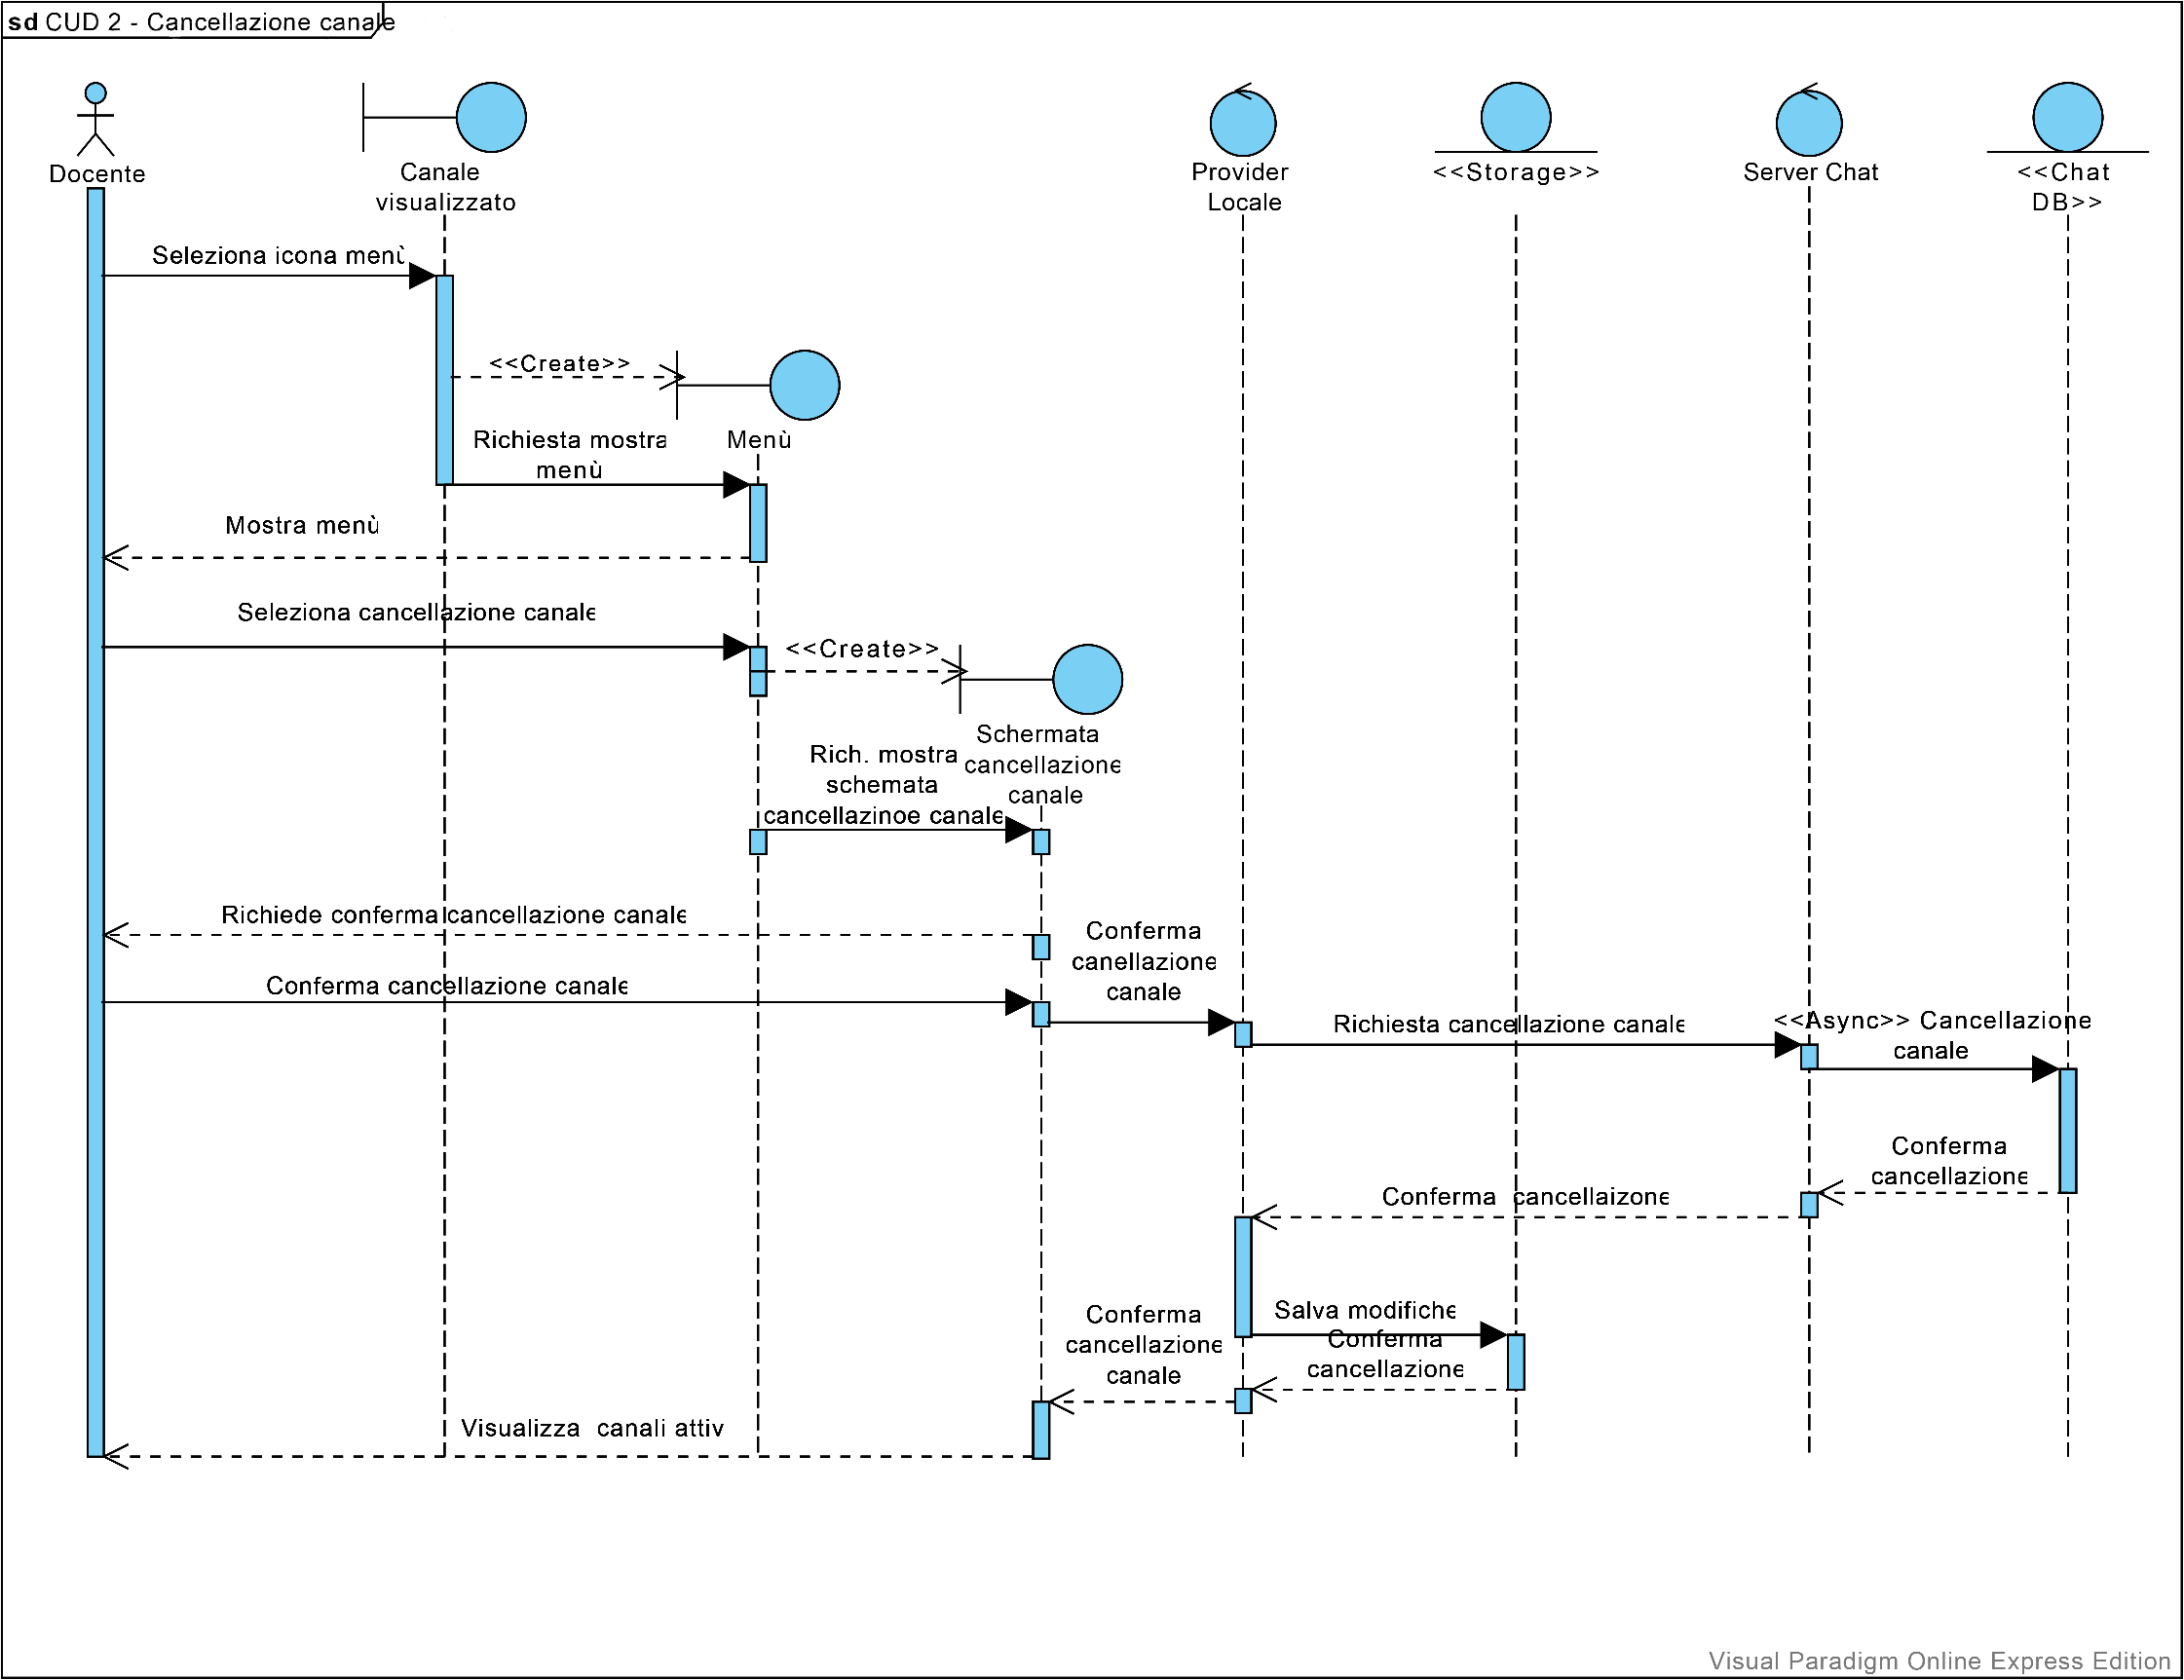
\includegraphics[width=0.9\textwidth]{imgs/gruppo6/sequence/CUD2_cancellazione_canale.pdf}
	\caption{CUD2 - Cancellazione canale}
	\label{fig:seq-cud2}
\end{figure}

\begin{figure}
	\centering
	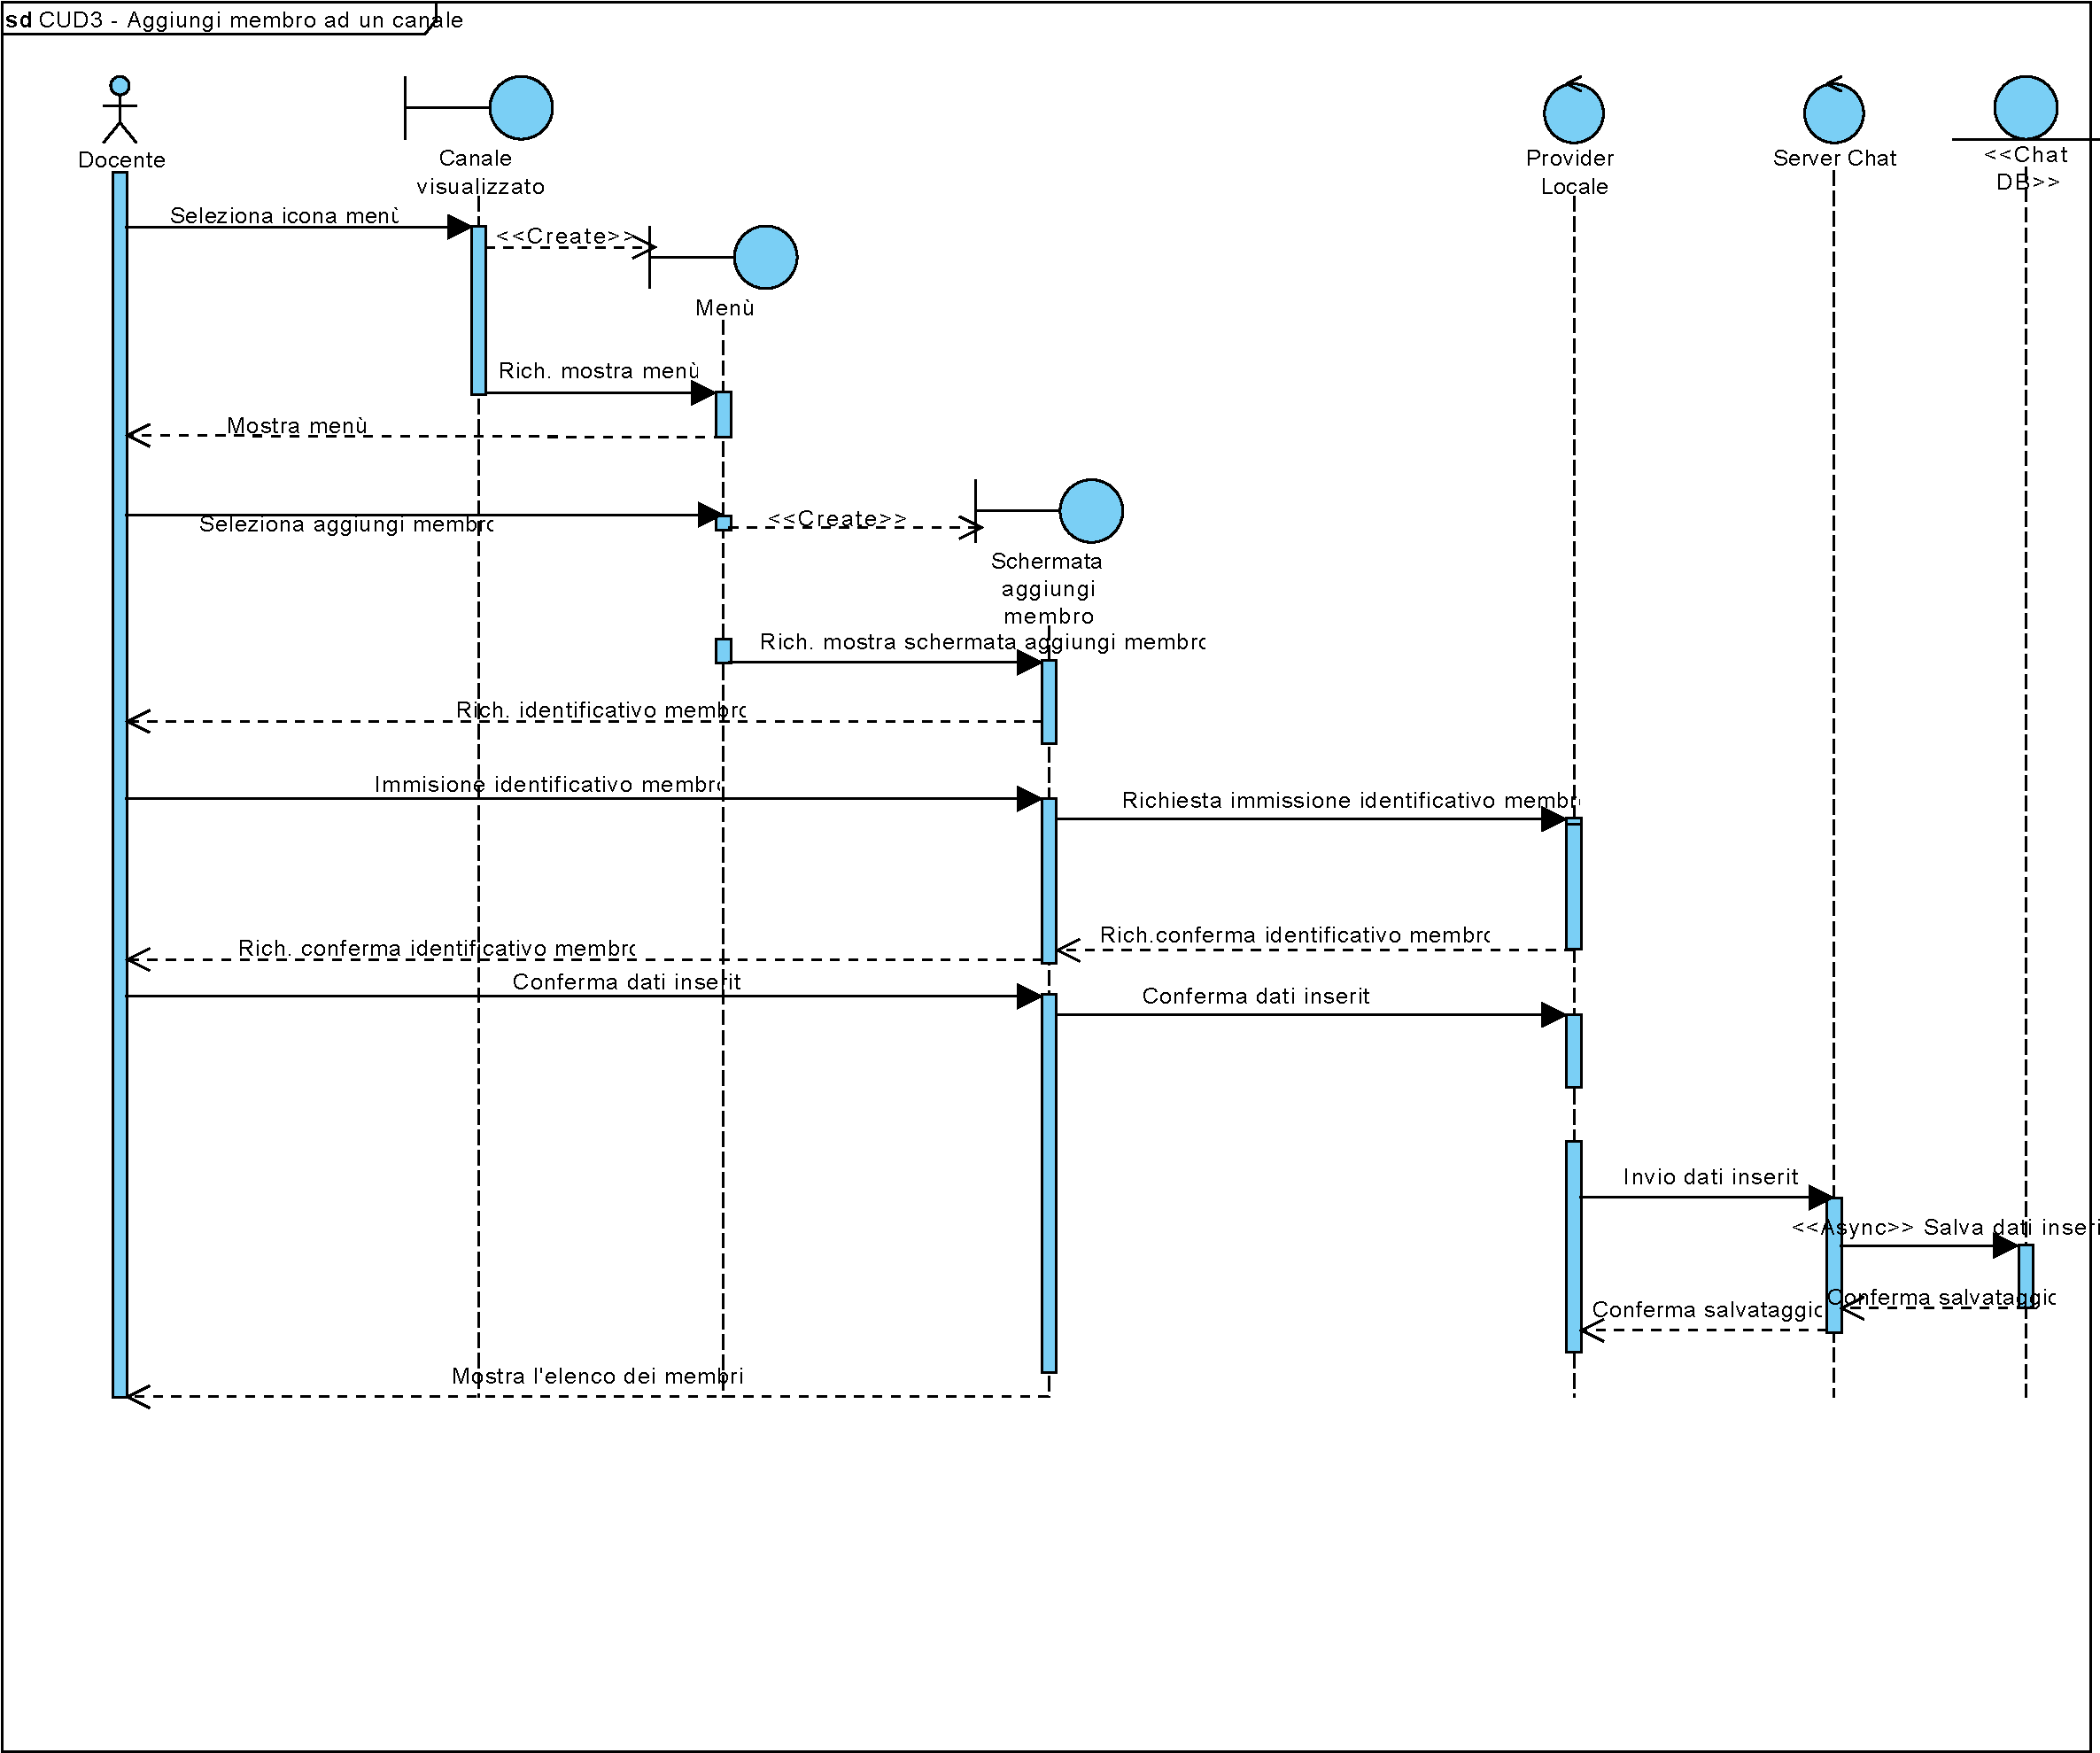
\includegraphics[width=0.9\textwidth]{imgs/gruppo6/sequence/CUD3_aggiungi_membro_ad_un_canale.pdf}
	\caption{CUD3 - Aggiungi membro a messaggio}
	\label{fig:seq-cud3}
\end{figure}

\begin{figure}
	\centering
	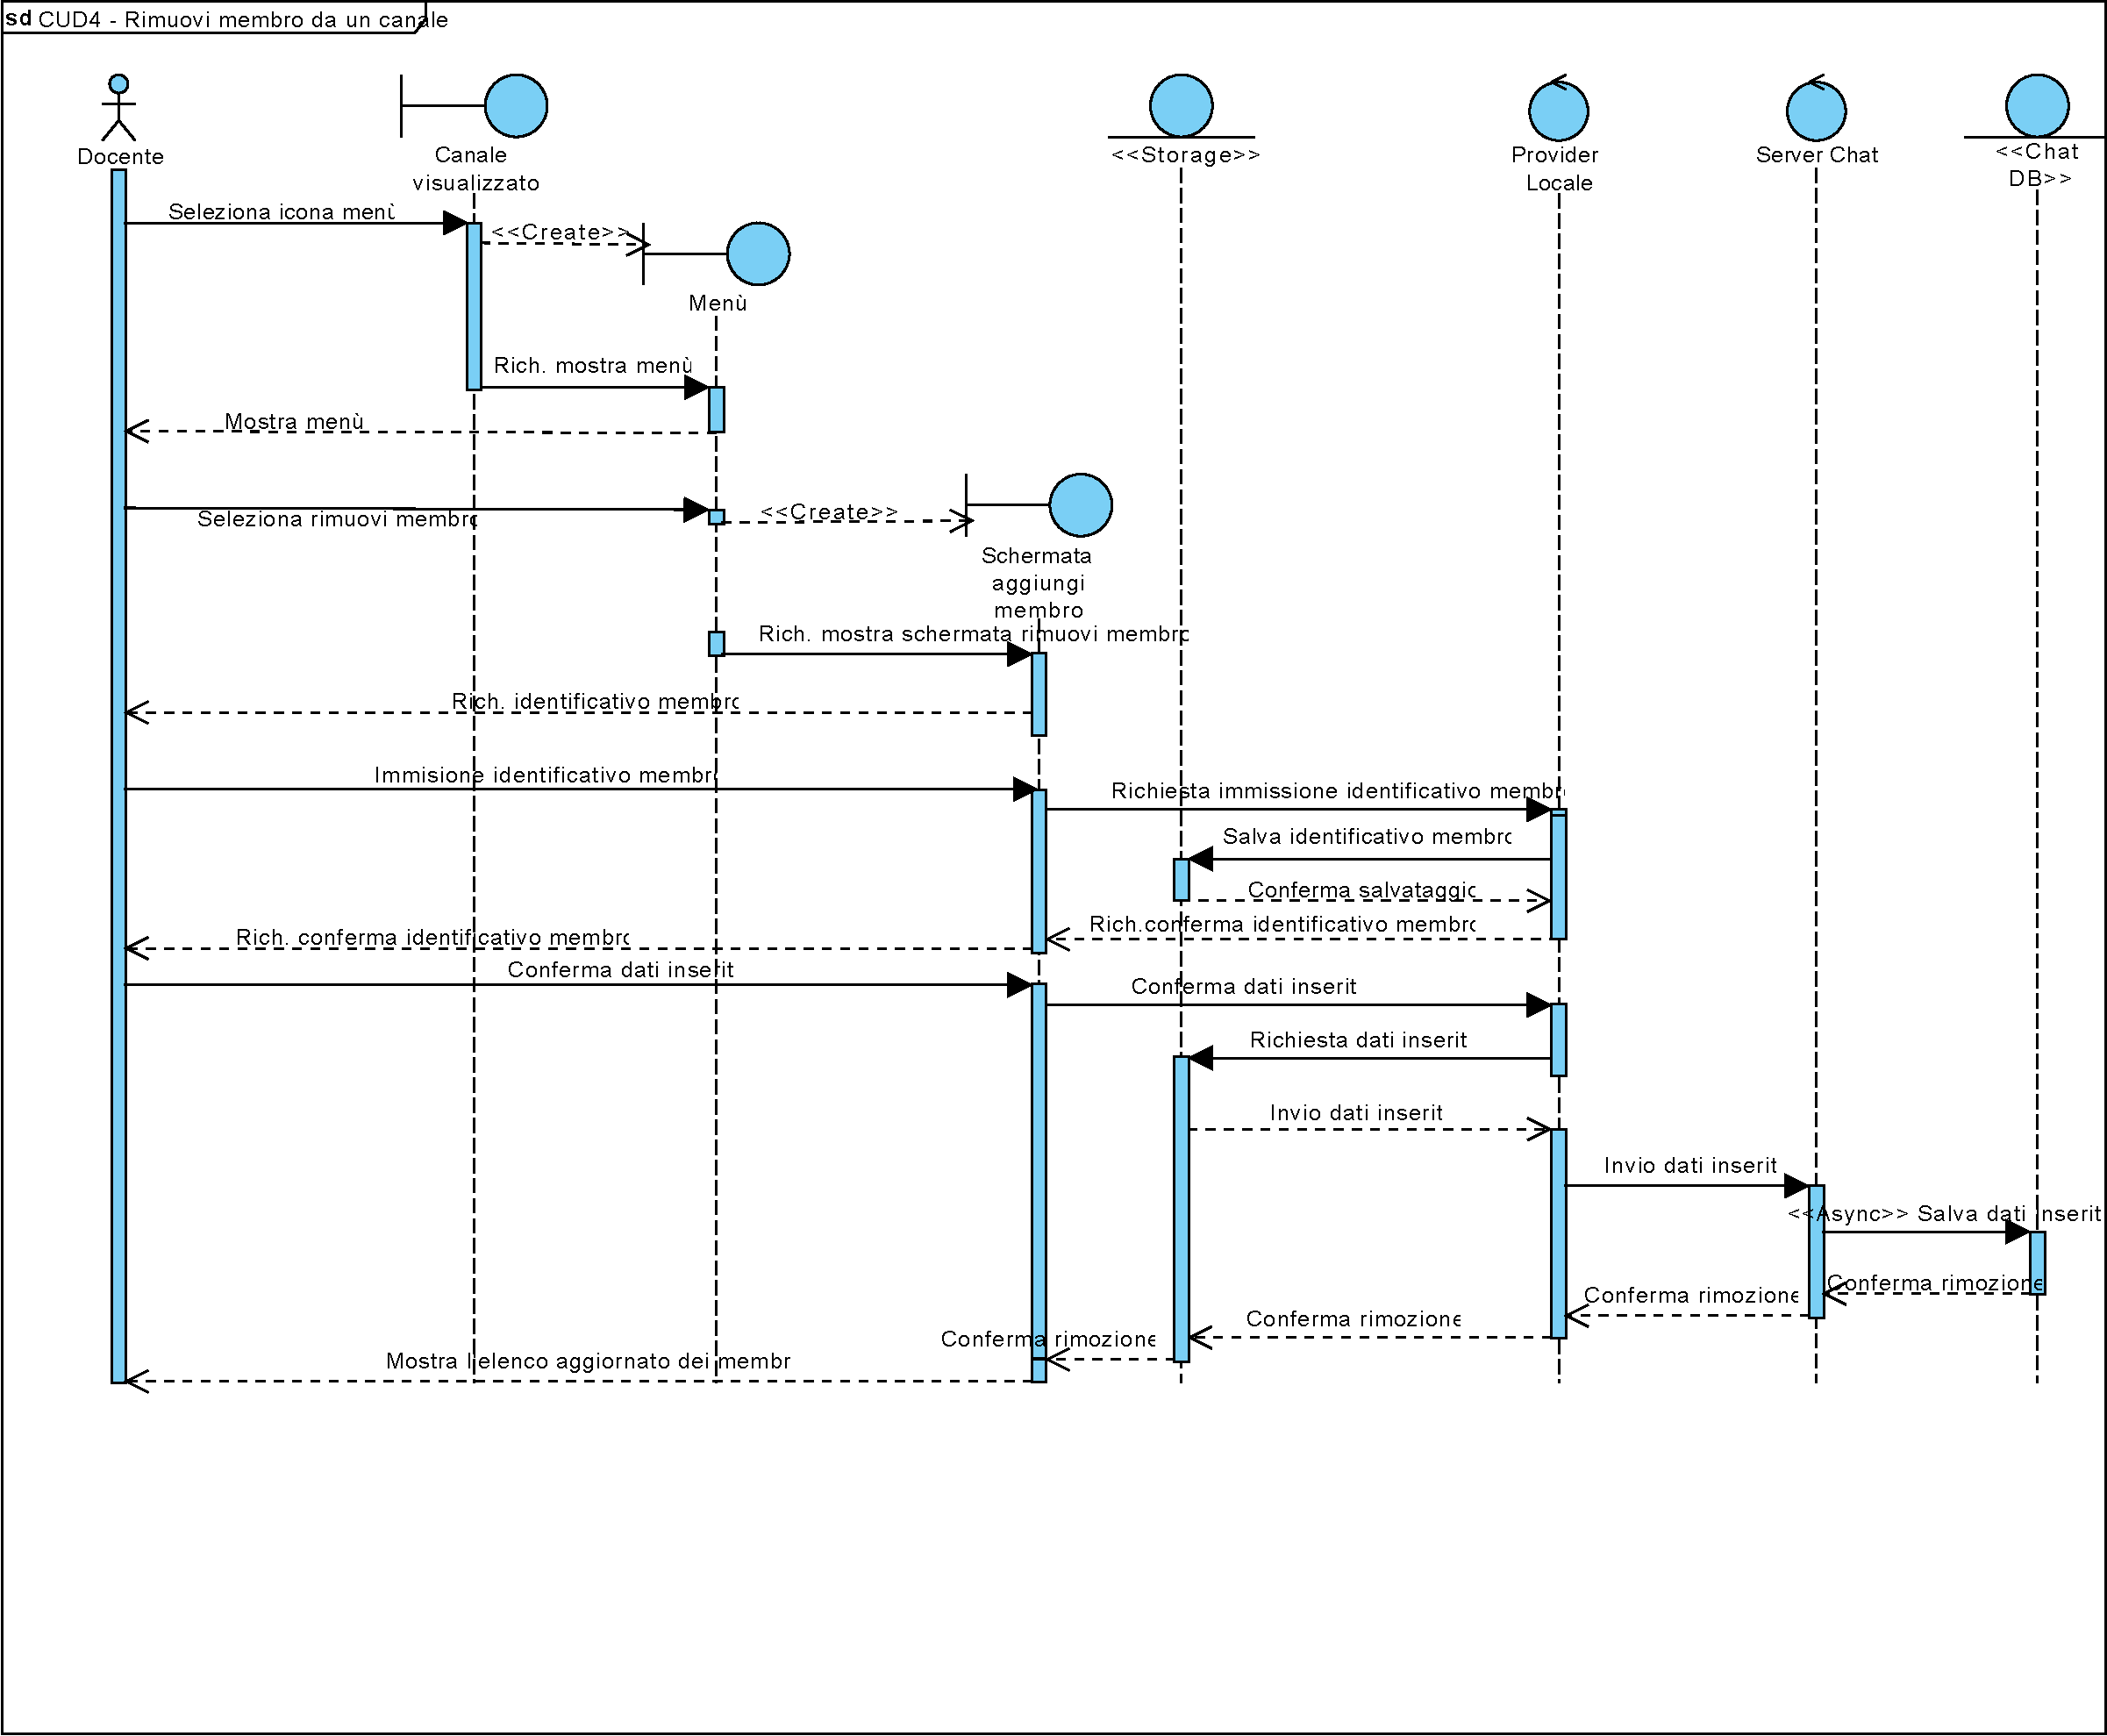
\includegraphics[width=0.9\textwidth]{imgs/gruppo6/sequence/CUD4_rimuovi_membro_ad_un_canale.pdf}
	\caption{CUD4 - Rimuovi membro ad un canale}
	\label{fig:seq-cud4}
\end{figure}

\begin{figure}
	\centering
	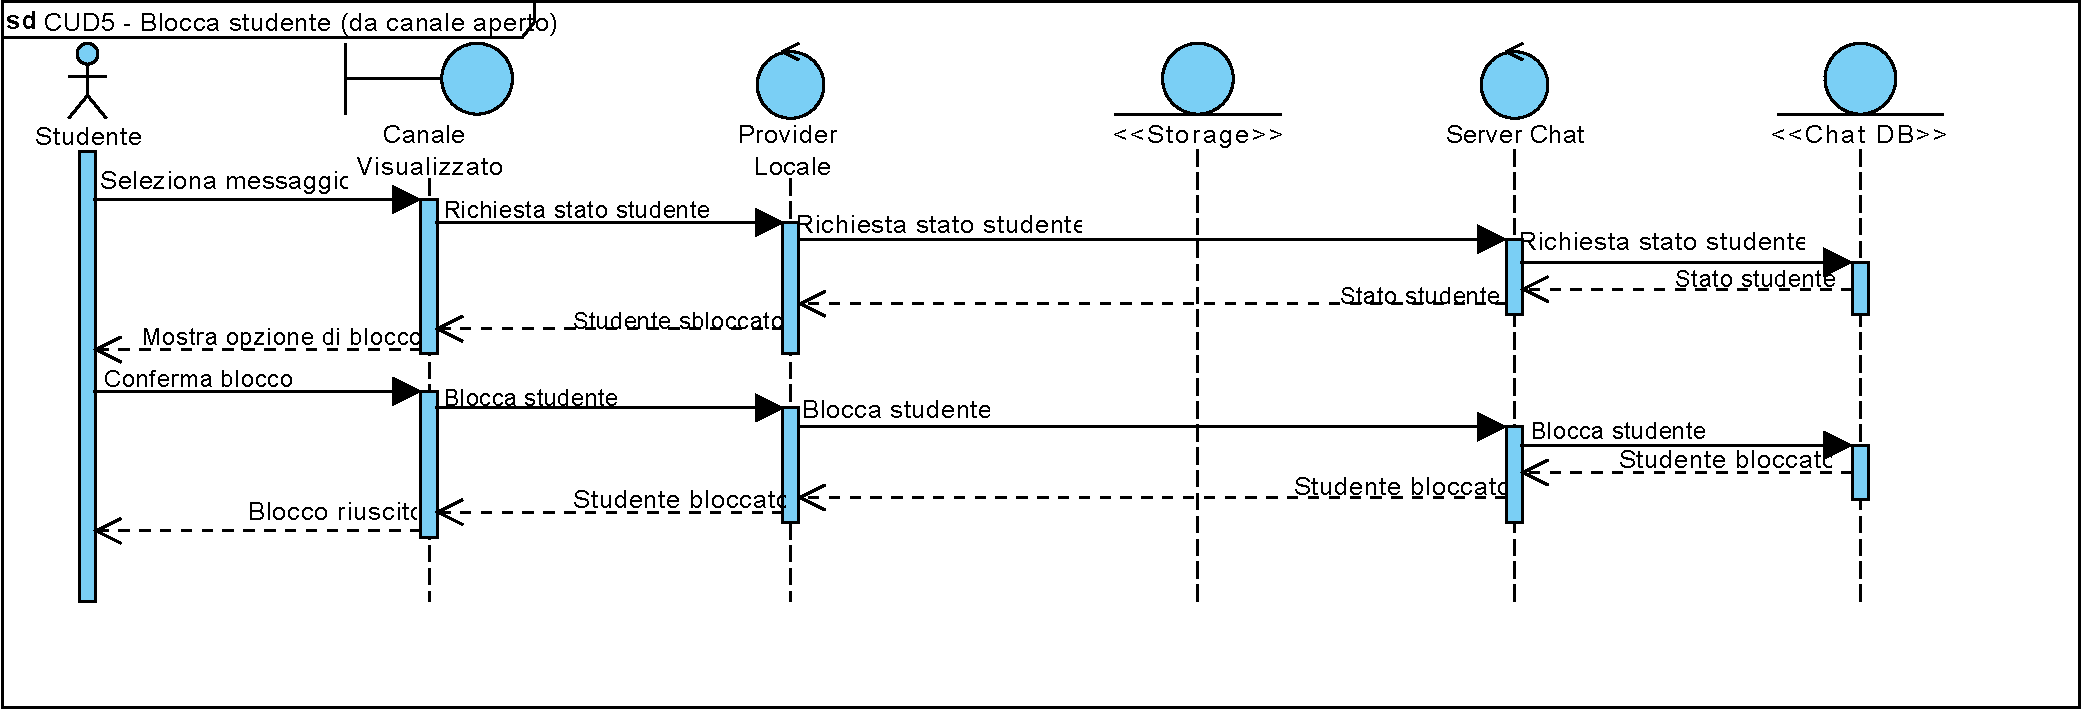
\includegraphics[width=0.9\textwidth]{imgs/gruppo6/sequence/CUD5_blocca_studente.pdf}
	\caption{CUD5 - Blocca studente}
	\label{fig:seq-cud5}
\end{figure}

\begin{figure}
	\centering
	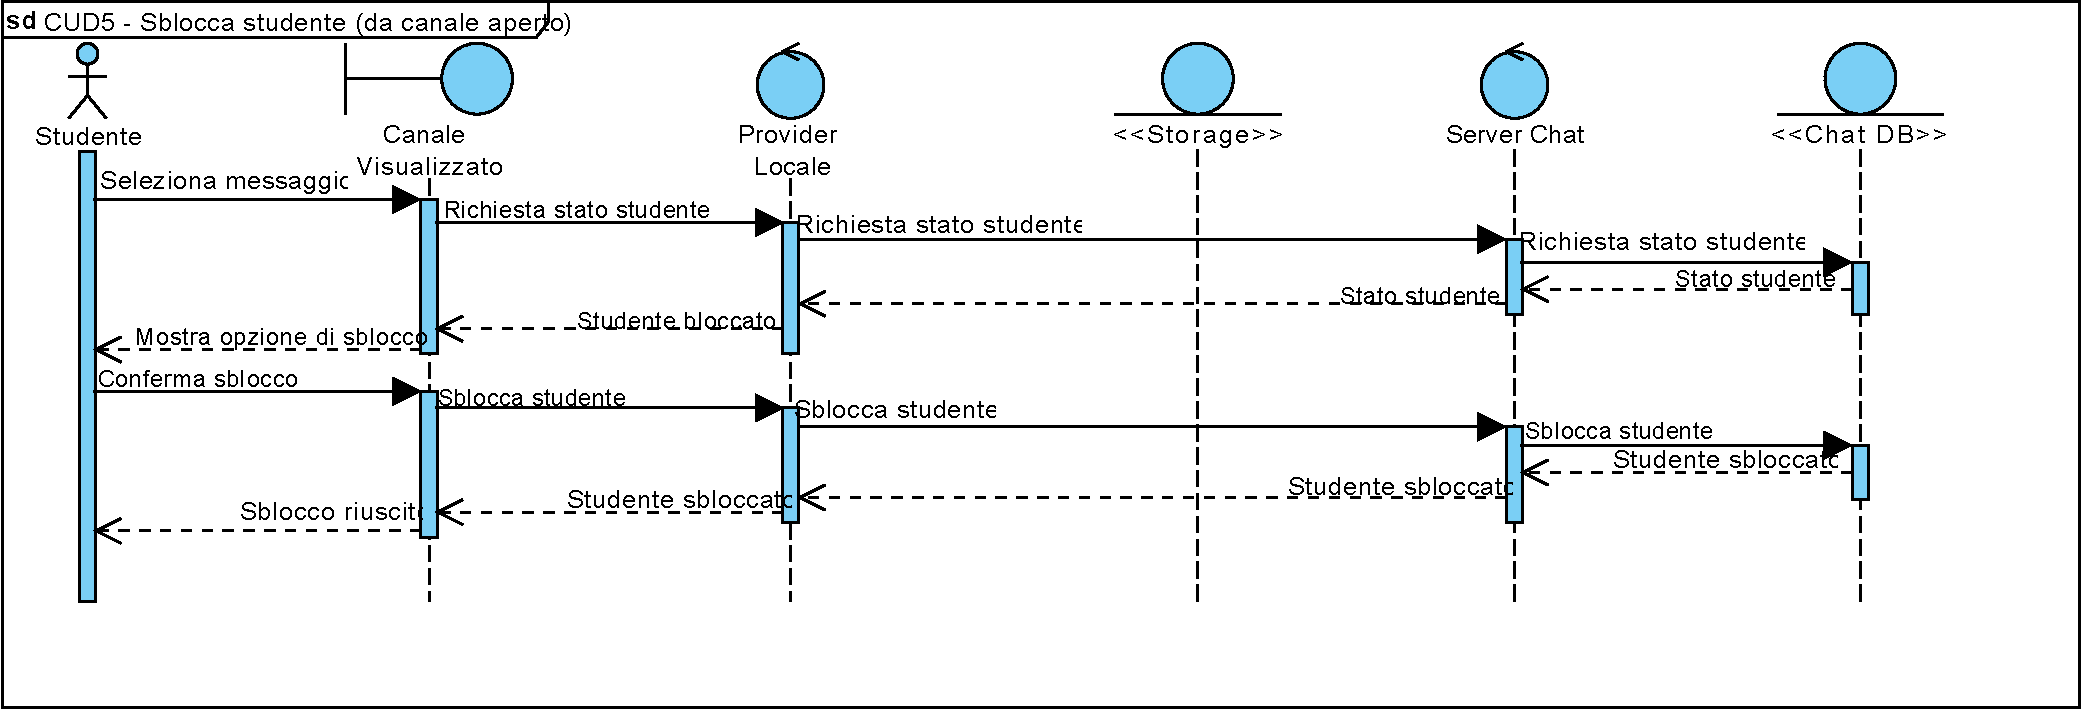
\includegraphics[width=0.9\textwidth]{imgs/gruppo6/sequence/CUD6_sblocca_studente.pdf}
	\caption{CUD6 - Sblocca studente}
	\label{fig:seq-cud6}
\end{figure}

\pagebreak

\begin{figure}[!h]
	\subsubsection{Pannello di amministrazione}
	\centering
	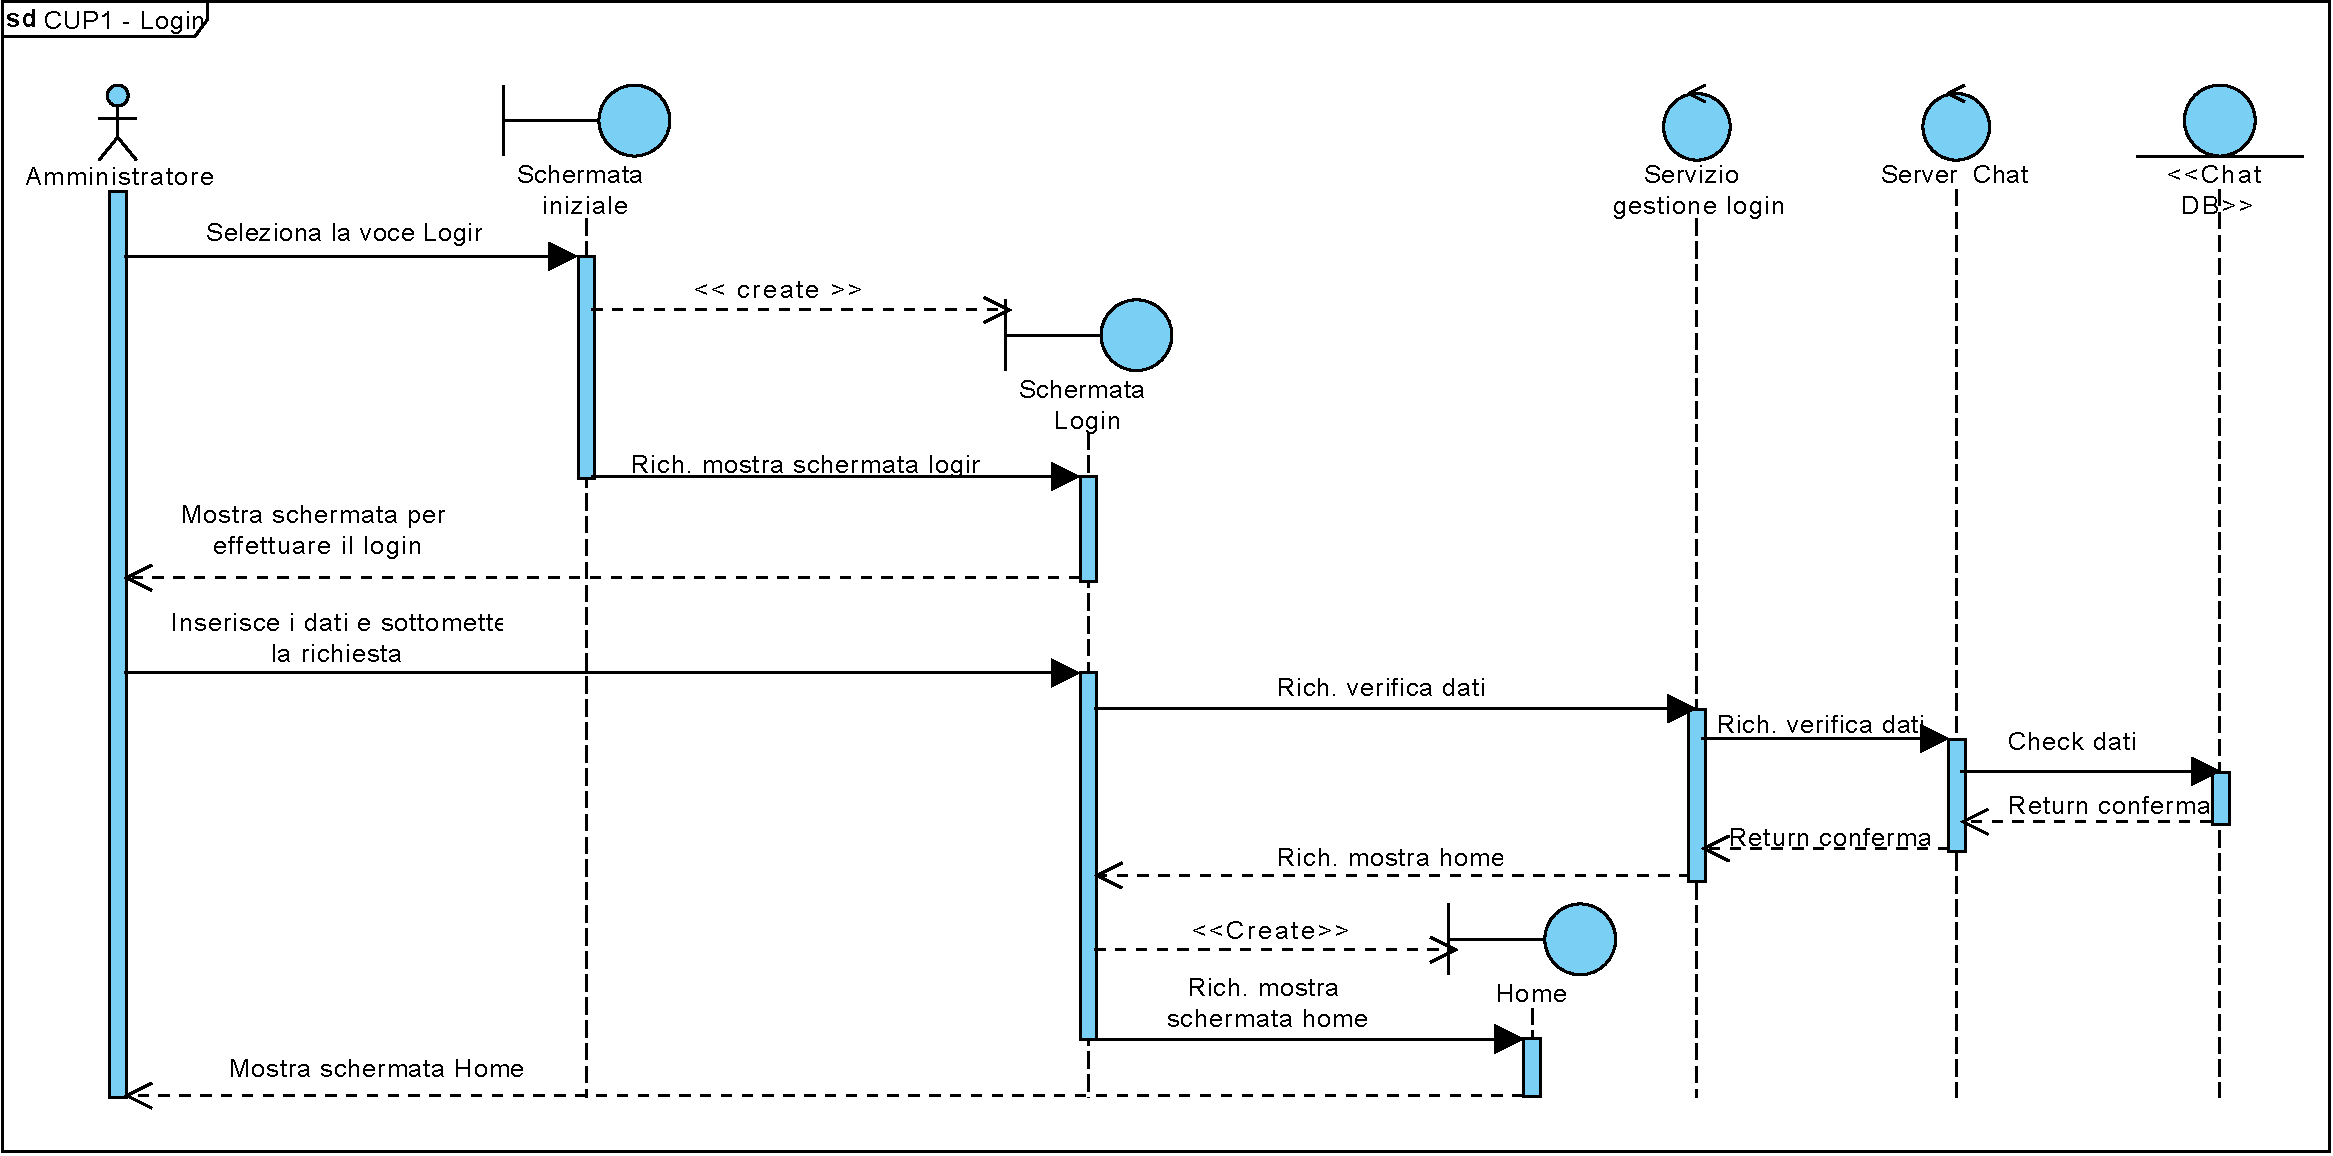
\includegraphics[width=0.9\textwidth]{imgs/gruppo6/sequence/CUP1_Login.pdf}
	\caption{CUP1 - Login}
	\label{fig:seq-cup1}
\end{figure}

\begin{figure}
	\centering
	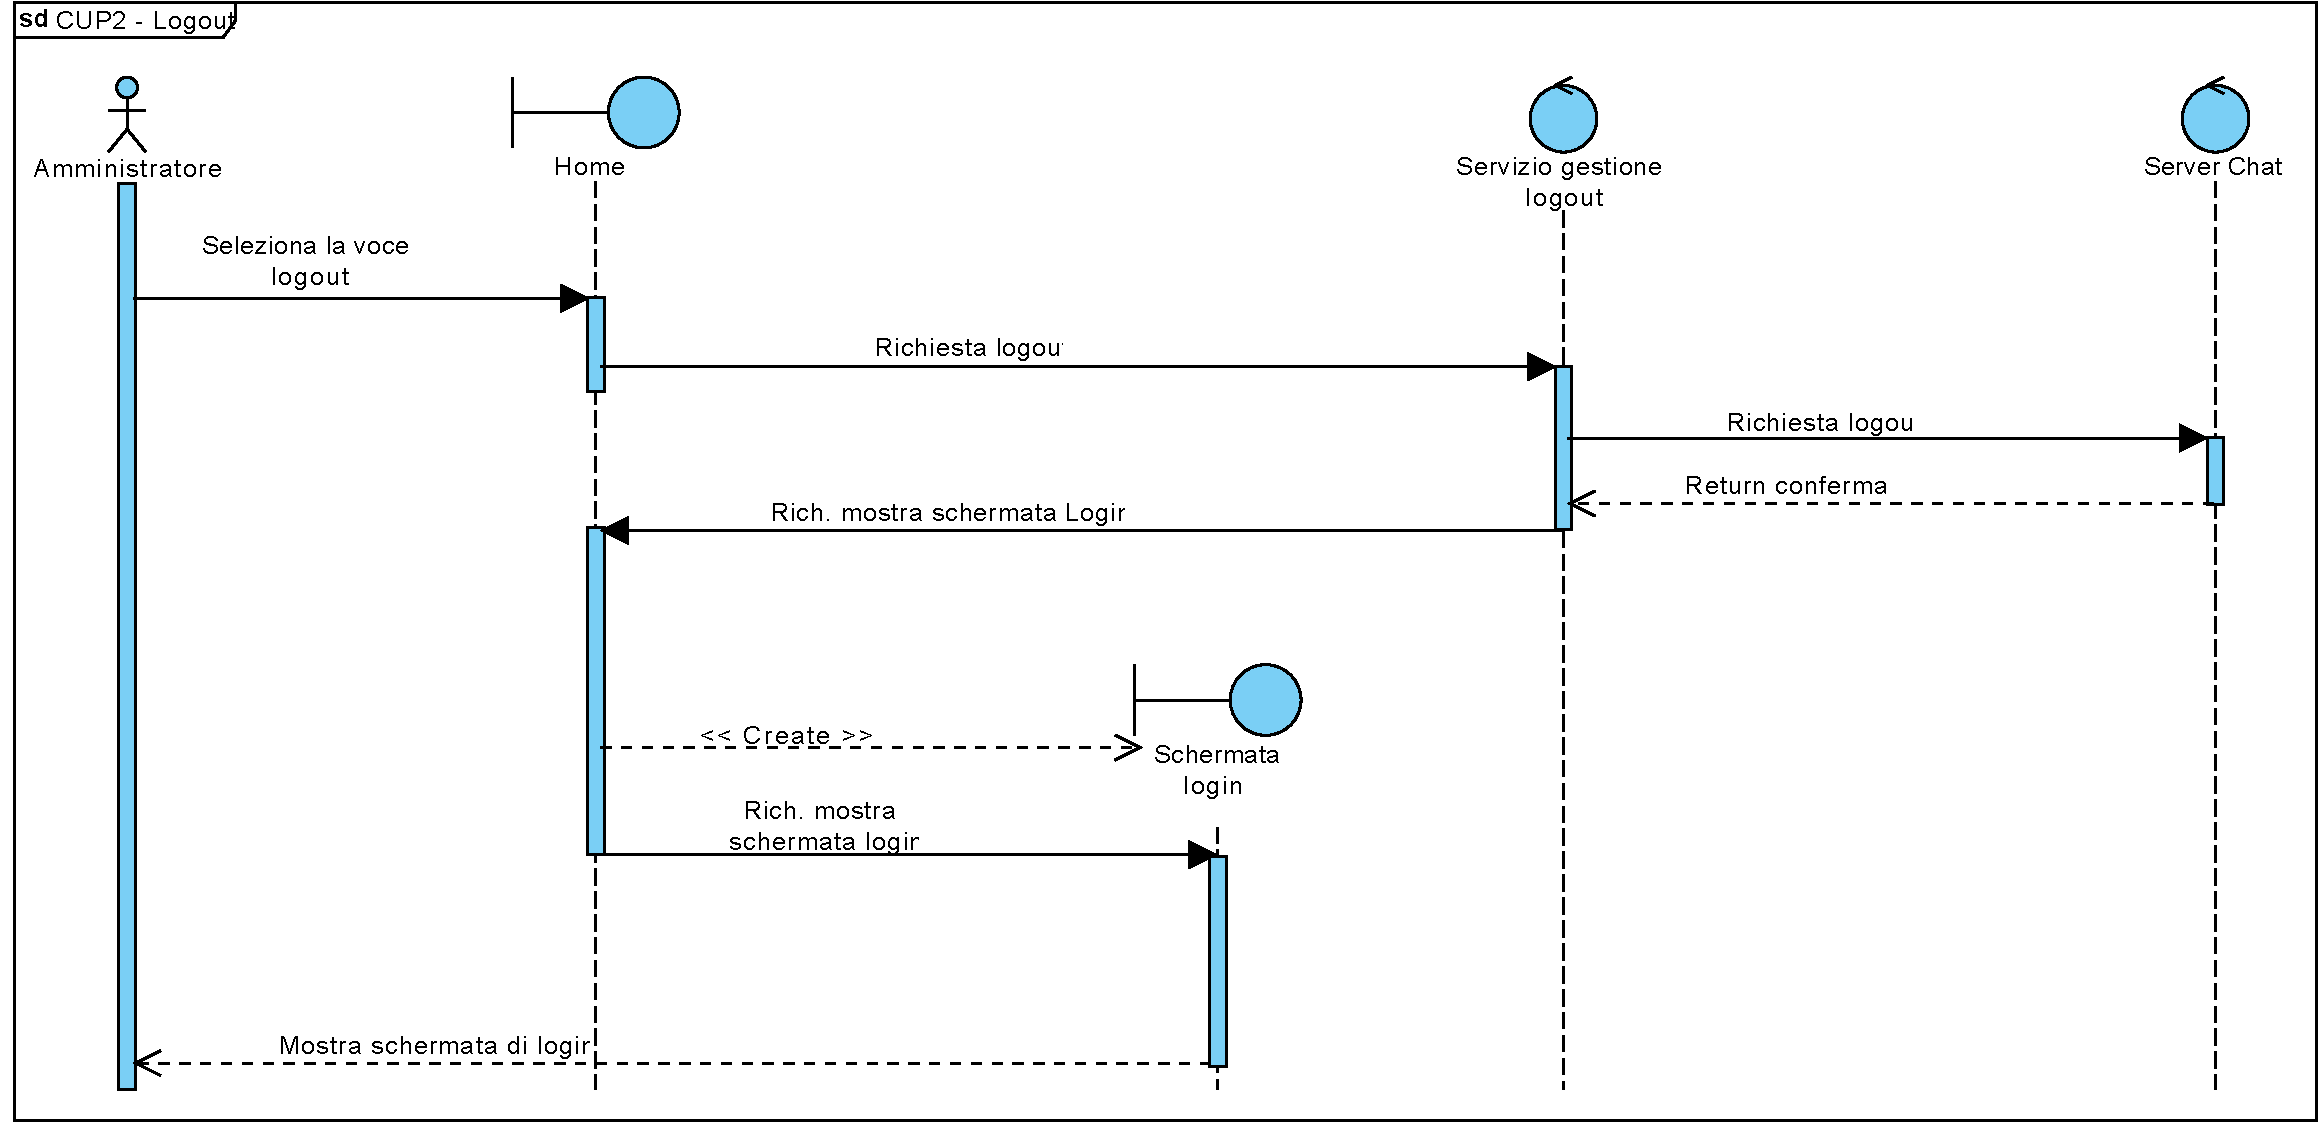
\includegraphics[width=0.9\textwidth]{imgs/gruppo6/sequence/CUP2_logout.pdf}
	\caption{CUP2 - Logout}
	\label{fig:seq-cup2}
\end{figure}

\begin{figure}
	\centering
	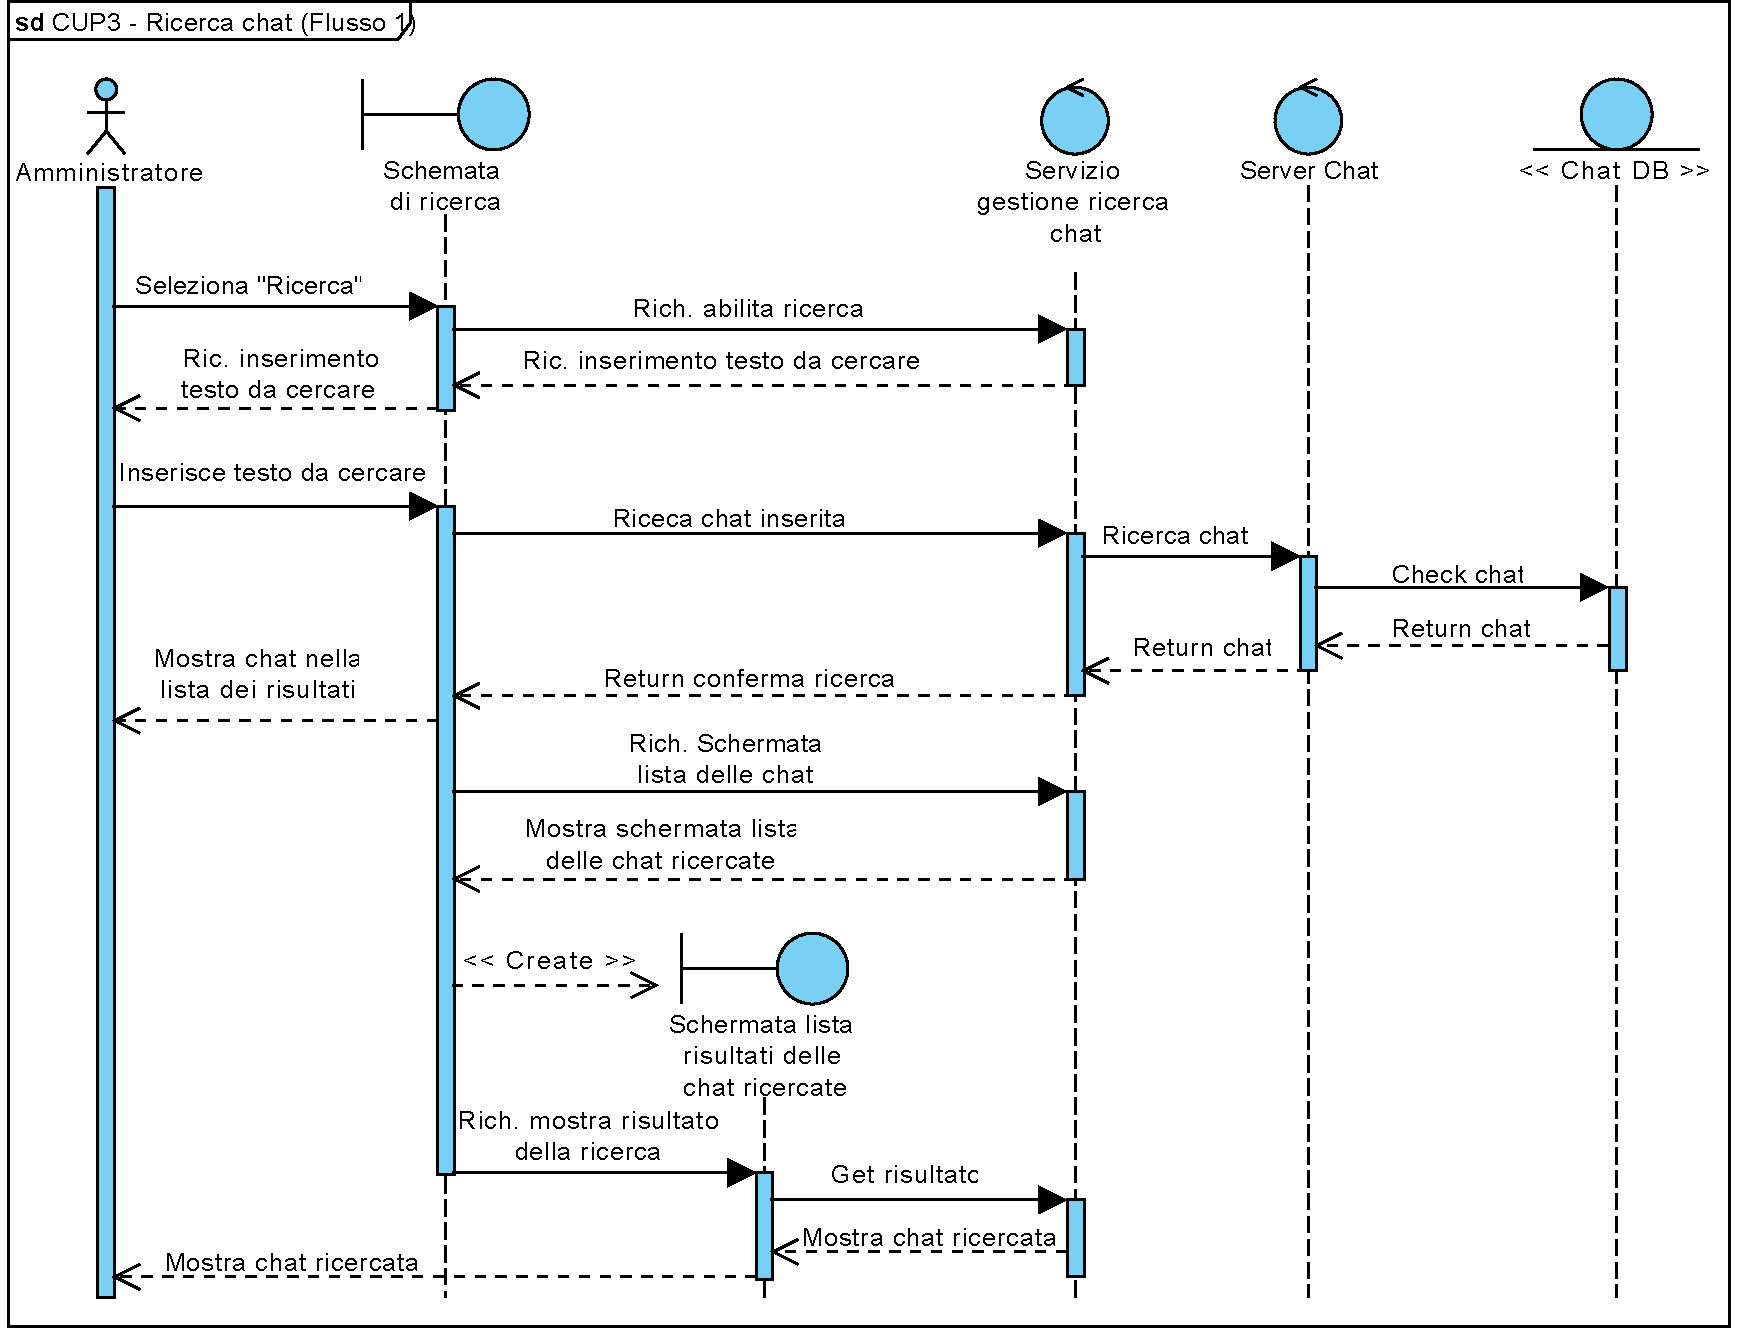
\includegraphics[width=0.9\textwidth]{imgs/gruppo6/sequence/CUP3_ricerca_chat_flusso_1.pdf}
	\caption{CUP3 - Ricerca chat}
	\label{fig:seq-cup3}
\end{figure}

\begin{figure}
	\centering
	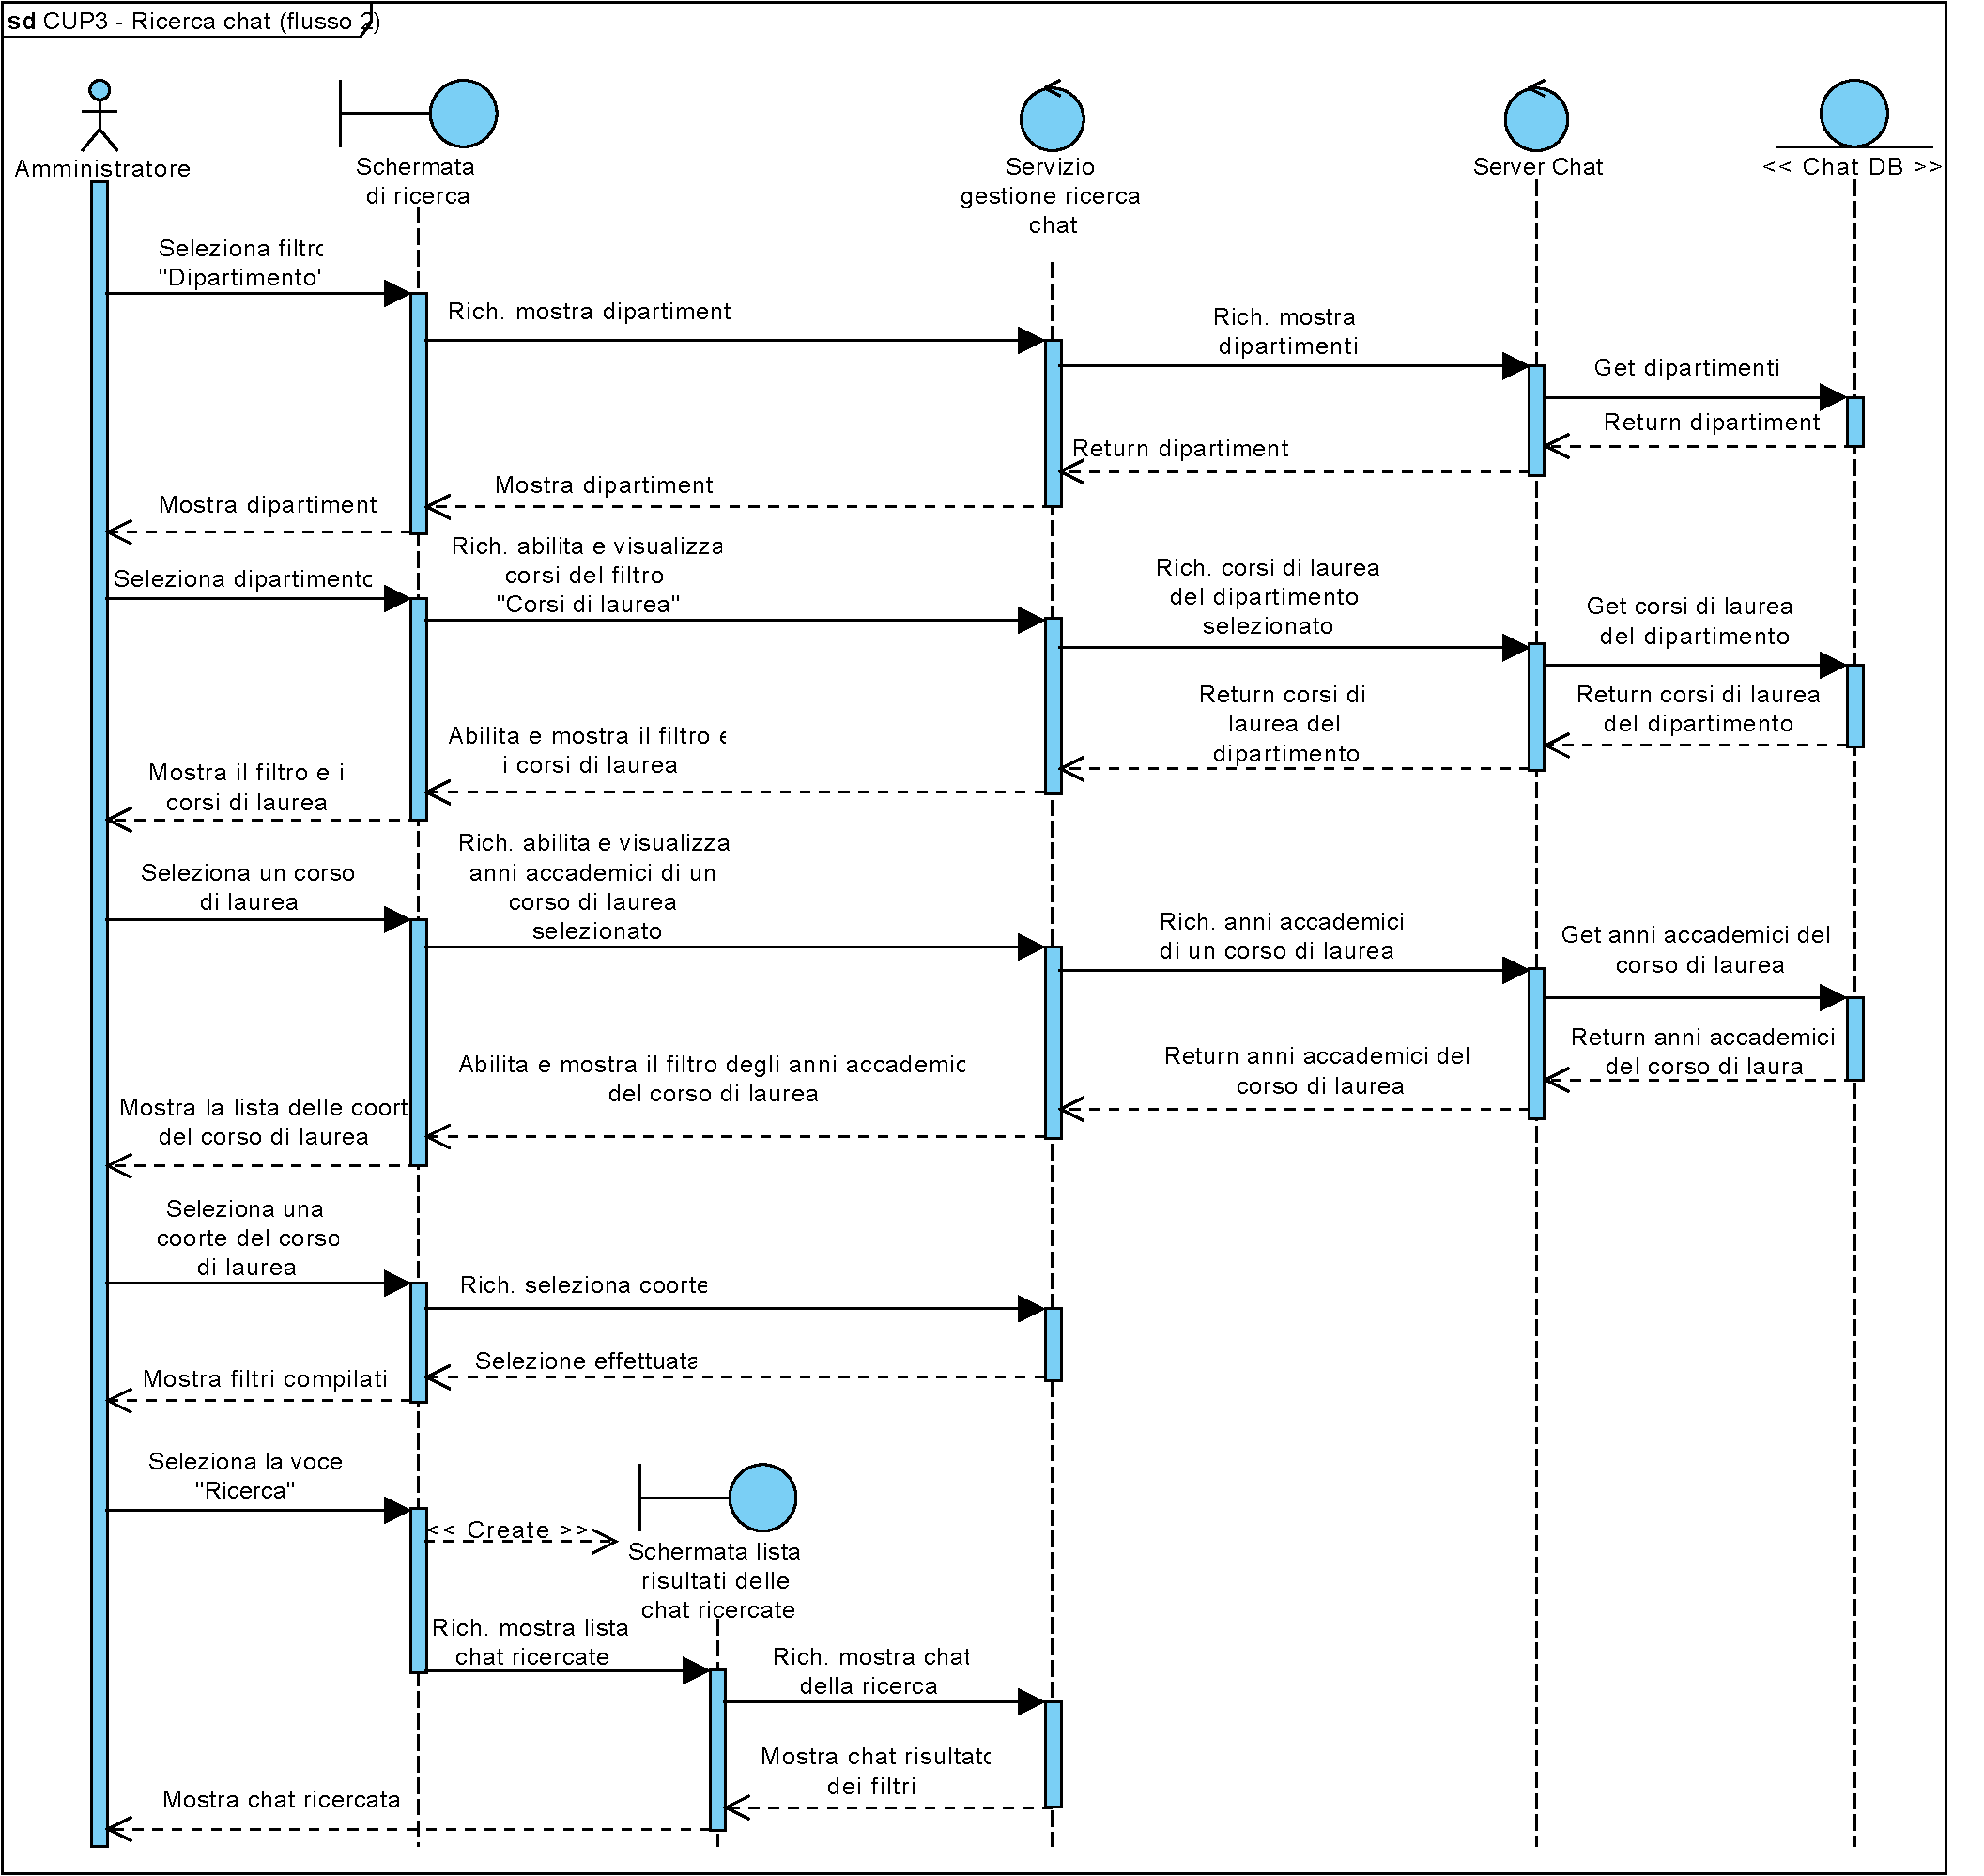
\includegraphics[width=0.9\textwidth]{imgs/gruppo6/sequence/CUP3_ricerca_chat_flusso_2.pdf}
	\caption{CUP3.1 - Ricerca chat flusso alternativo}
	\label{fig:seq-cup3mod}
\end{figure}

\begin{figure}
	\centering
	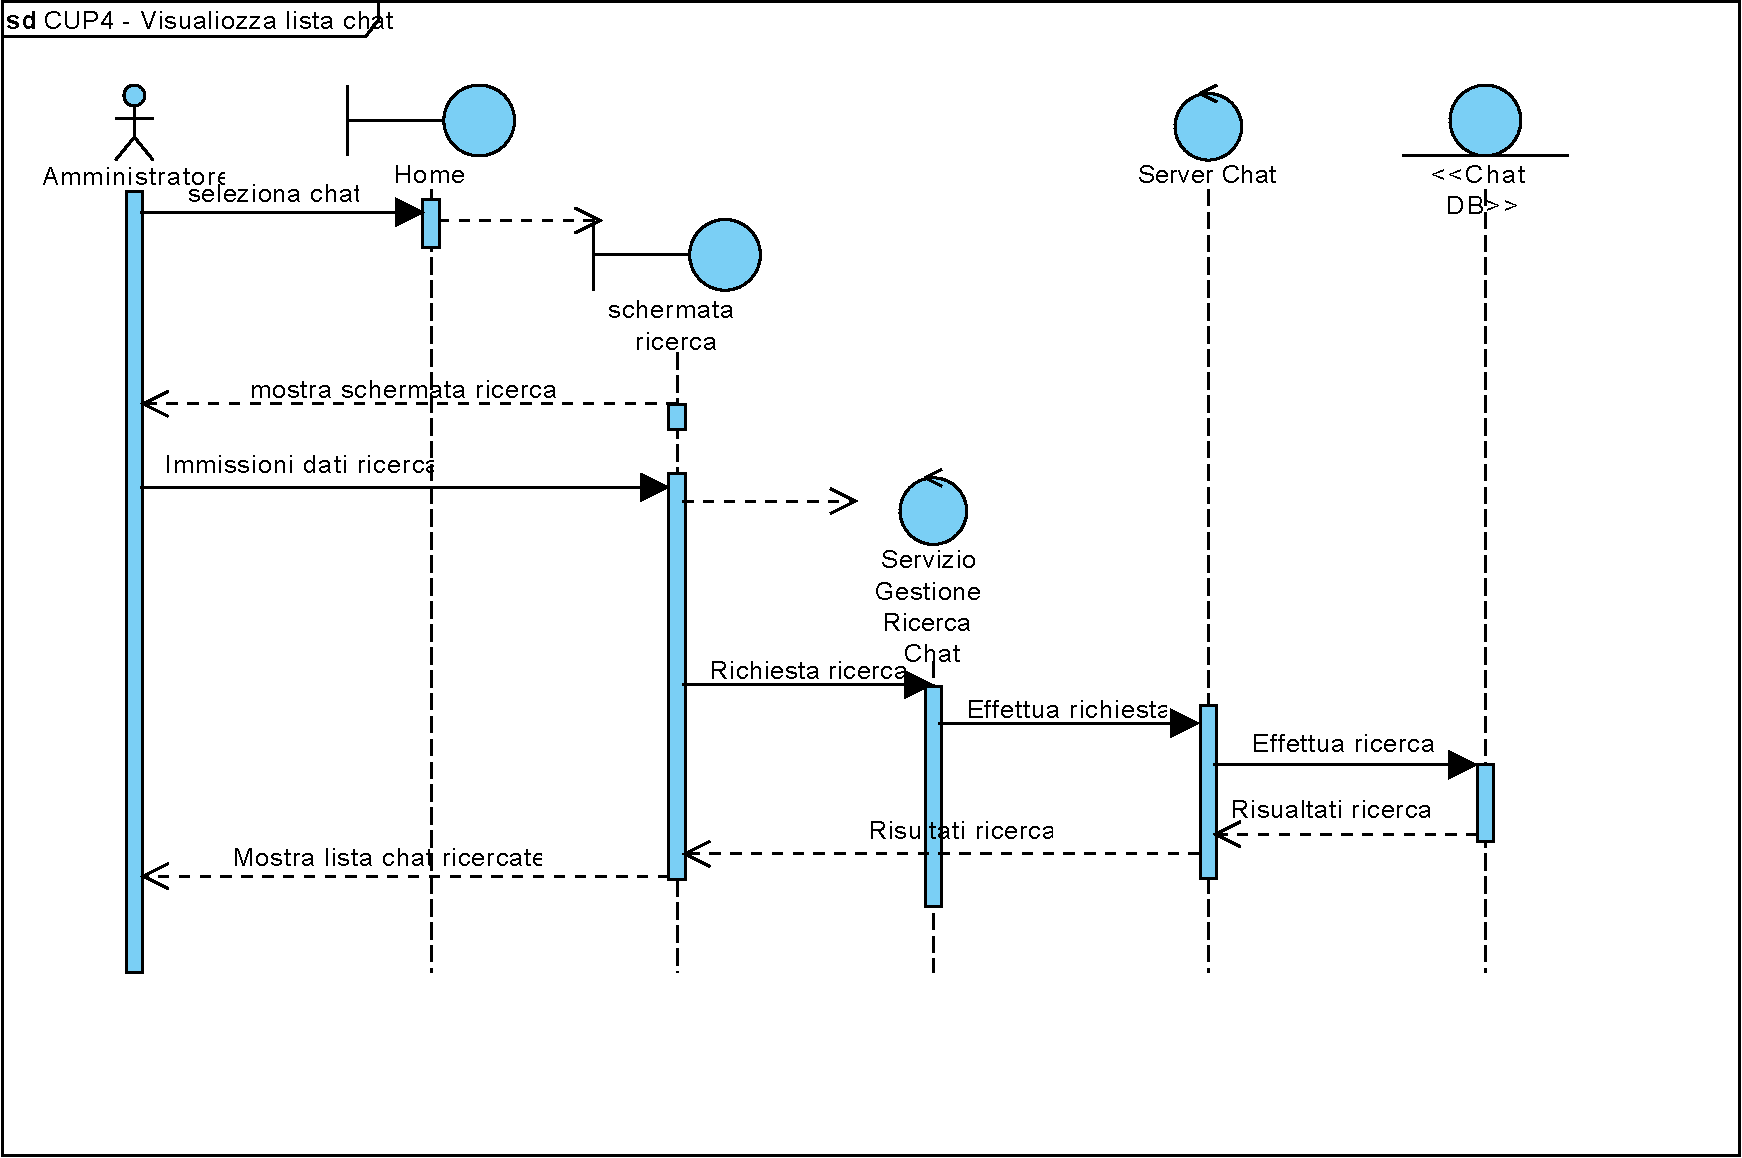
\includegraphics[width=0.9\textwidth]{imgs/gruppo6/sequence/CUP4_visualizza_lista_chat.pdf}
	\caption{CUP4 - Visualizza lista chat}
	\label{fig:seq-cup4}
\end{figure}

\begin{figure}
	\centering
	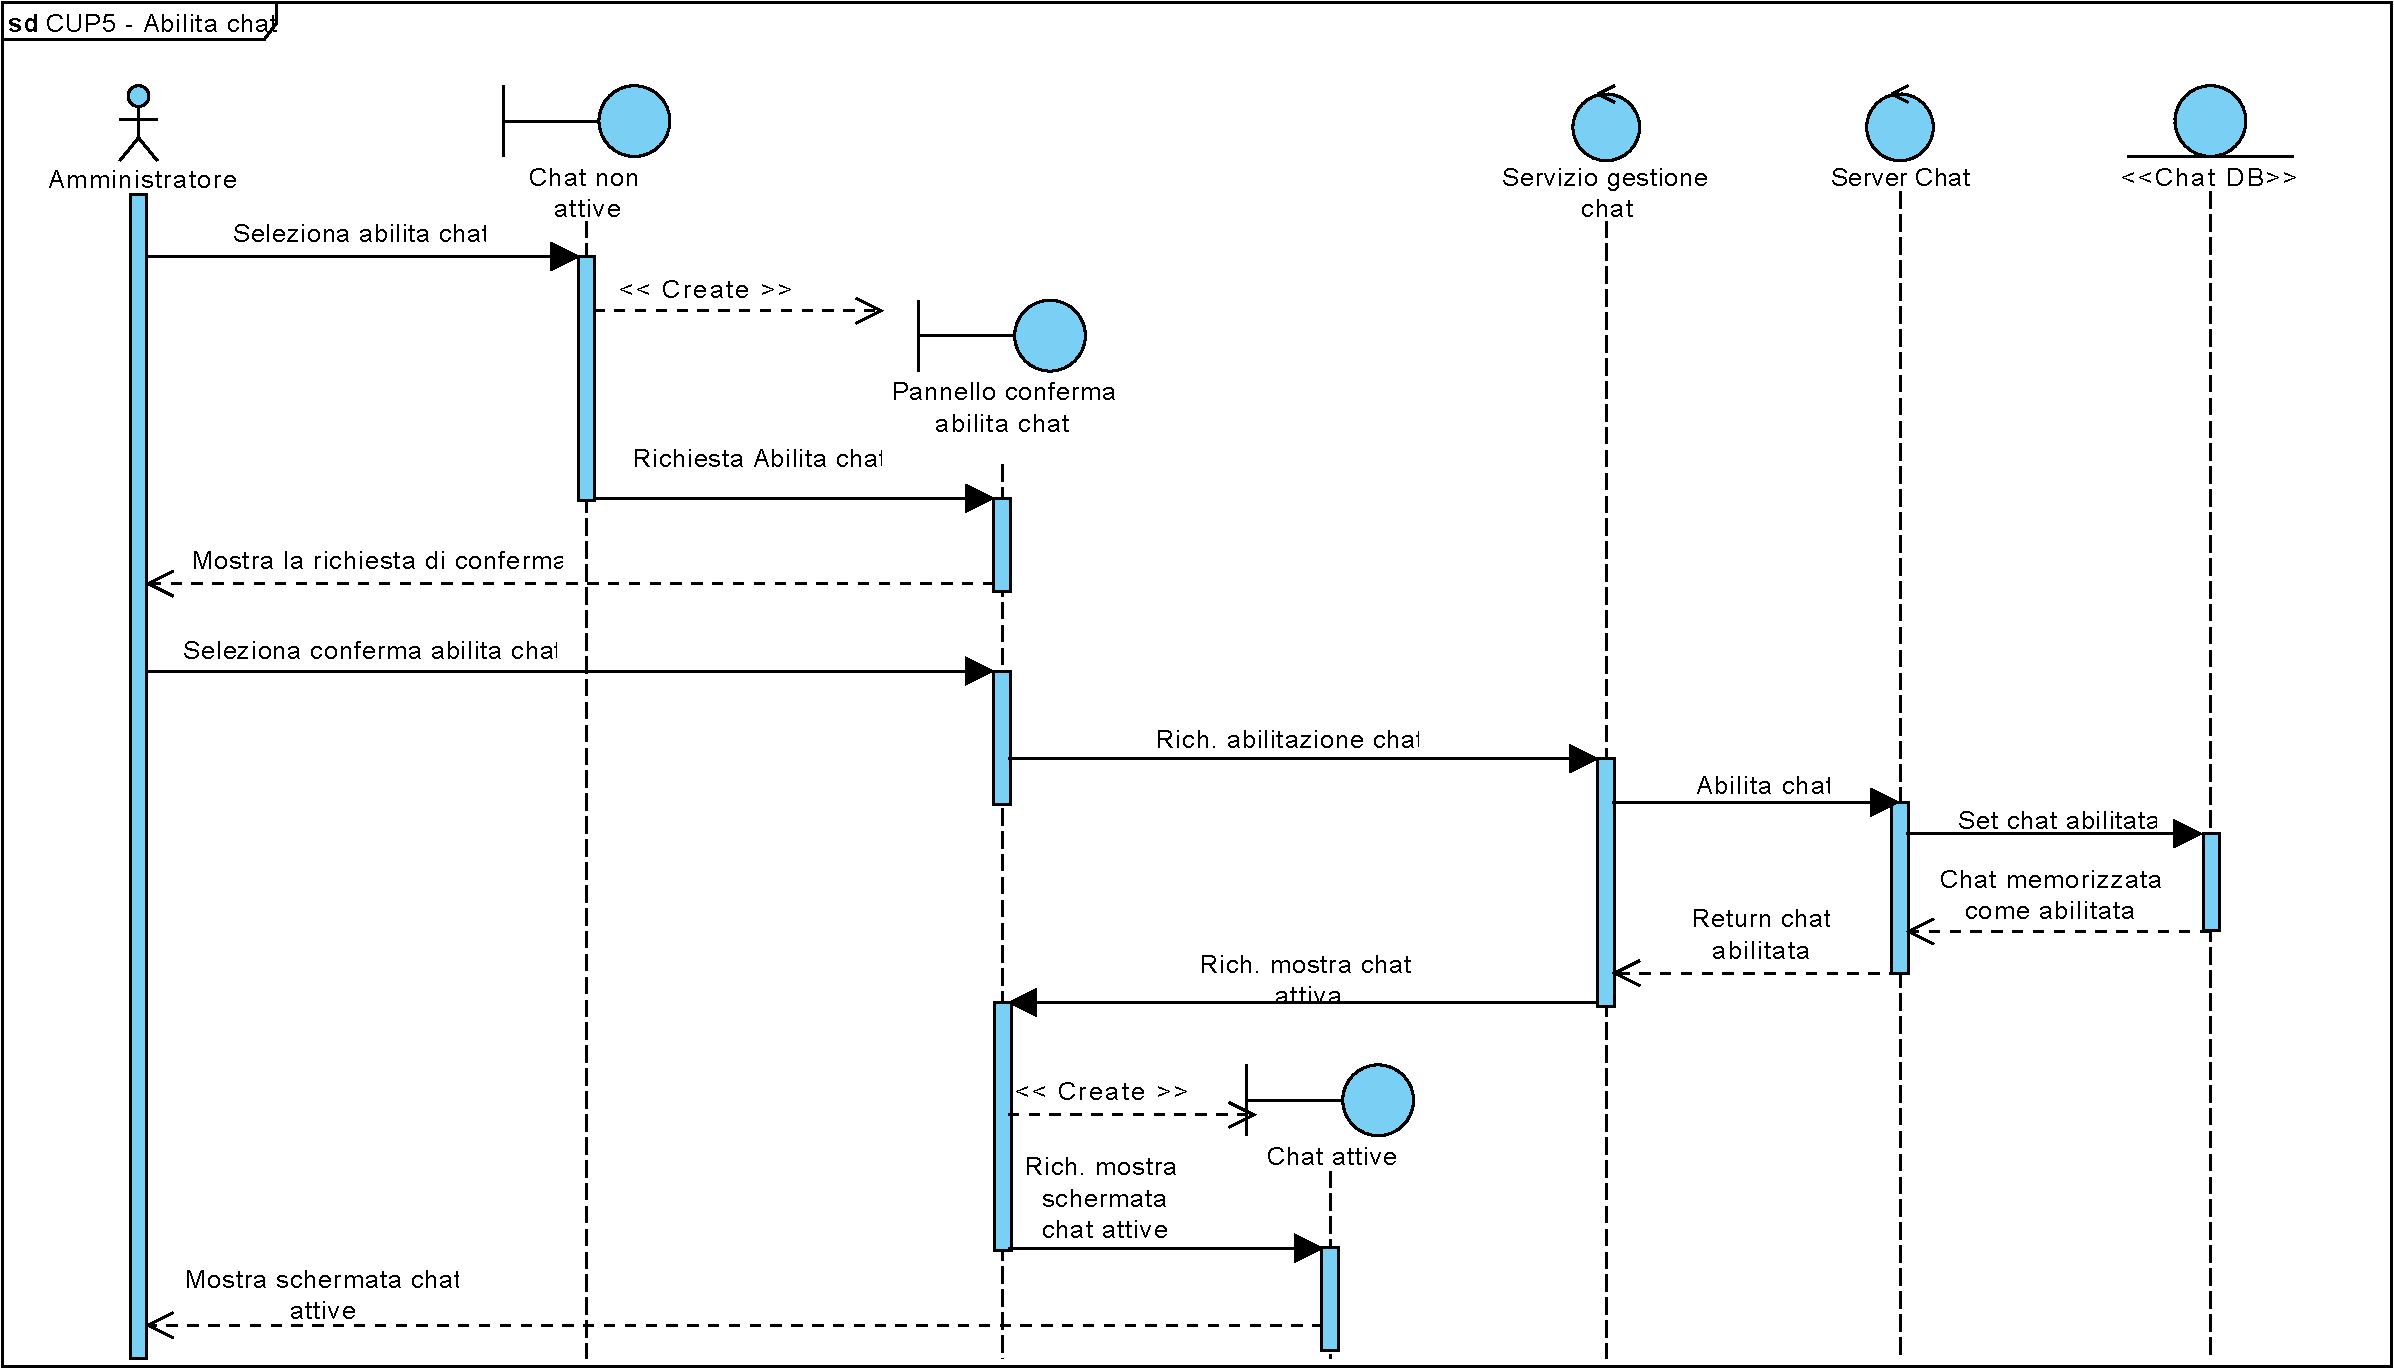
\includegraphics[width=0.9\textwidth]{imgs/gruppo6/sequence/CUP5_abilita_chat.pdf}
	\caption{CUP5 - Abilita chat}
	\label{fig:seq-cup5}
\end{figure}

\begin{figure}
	\centering
	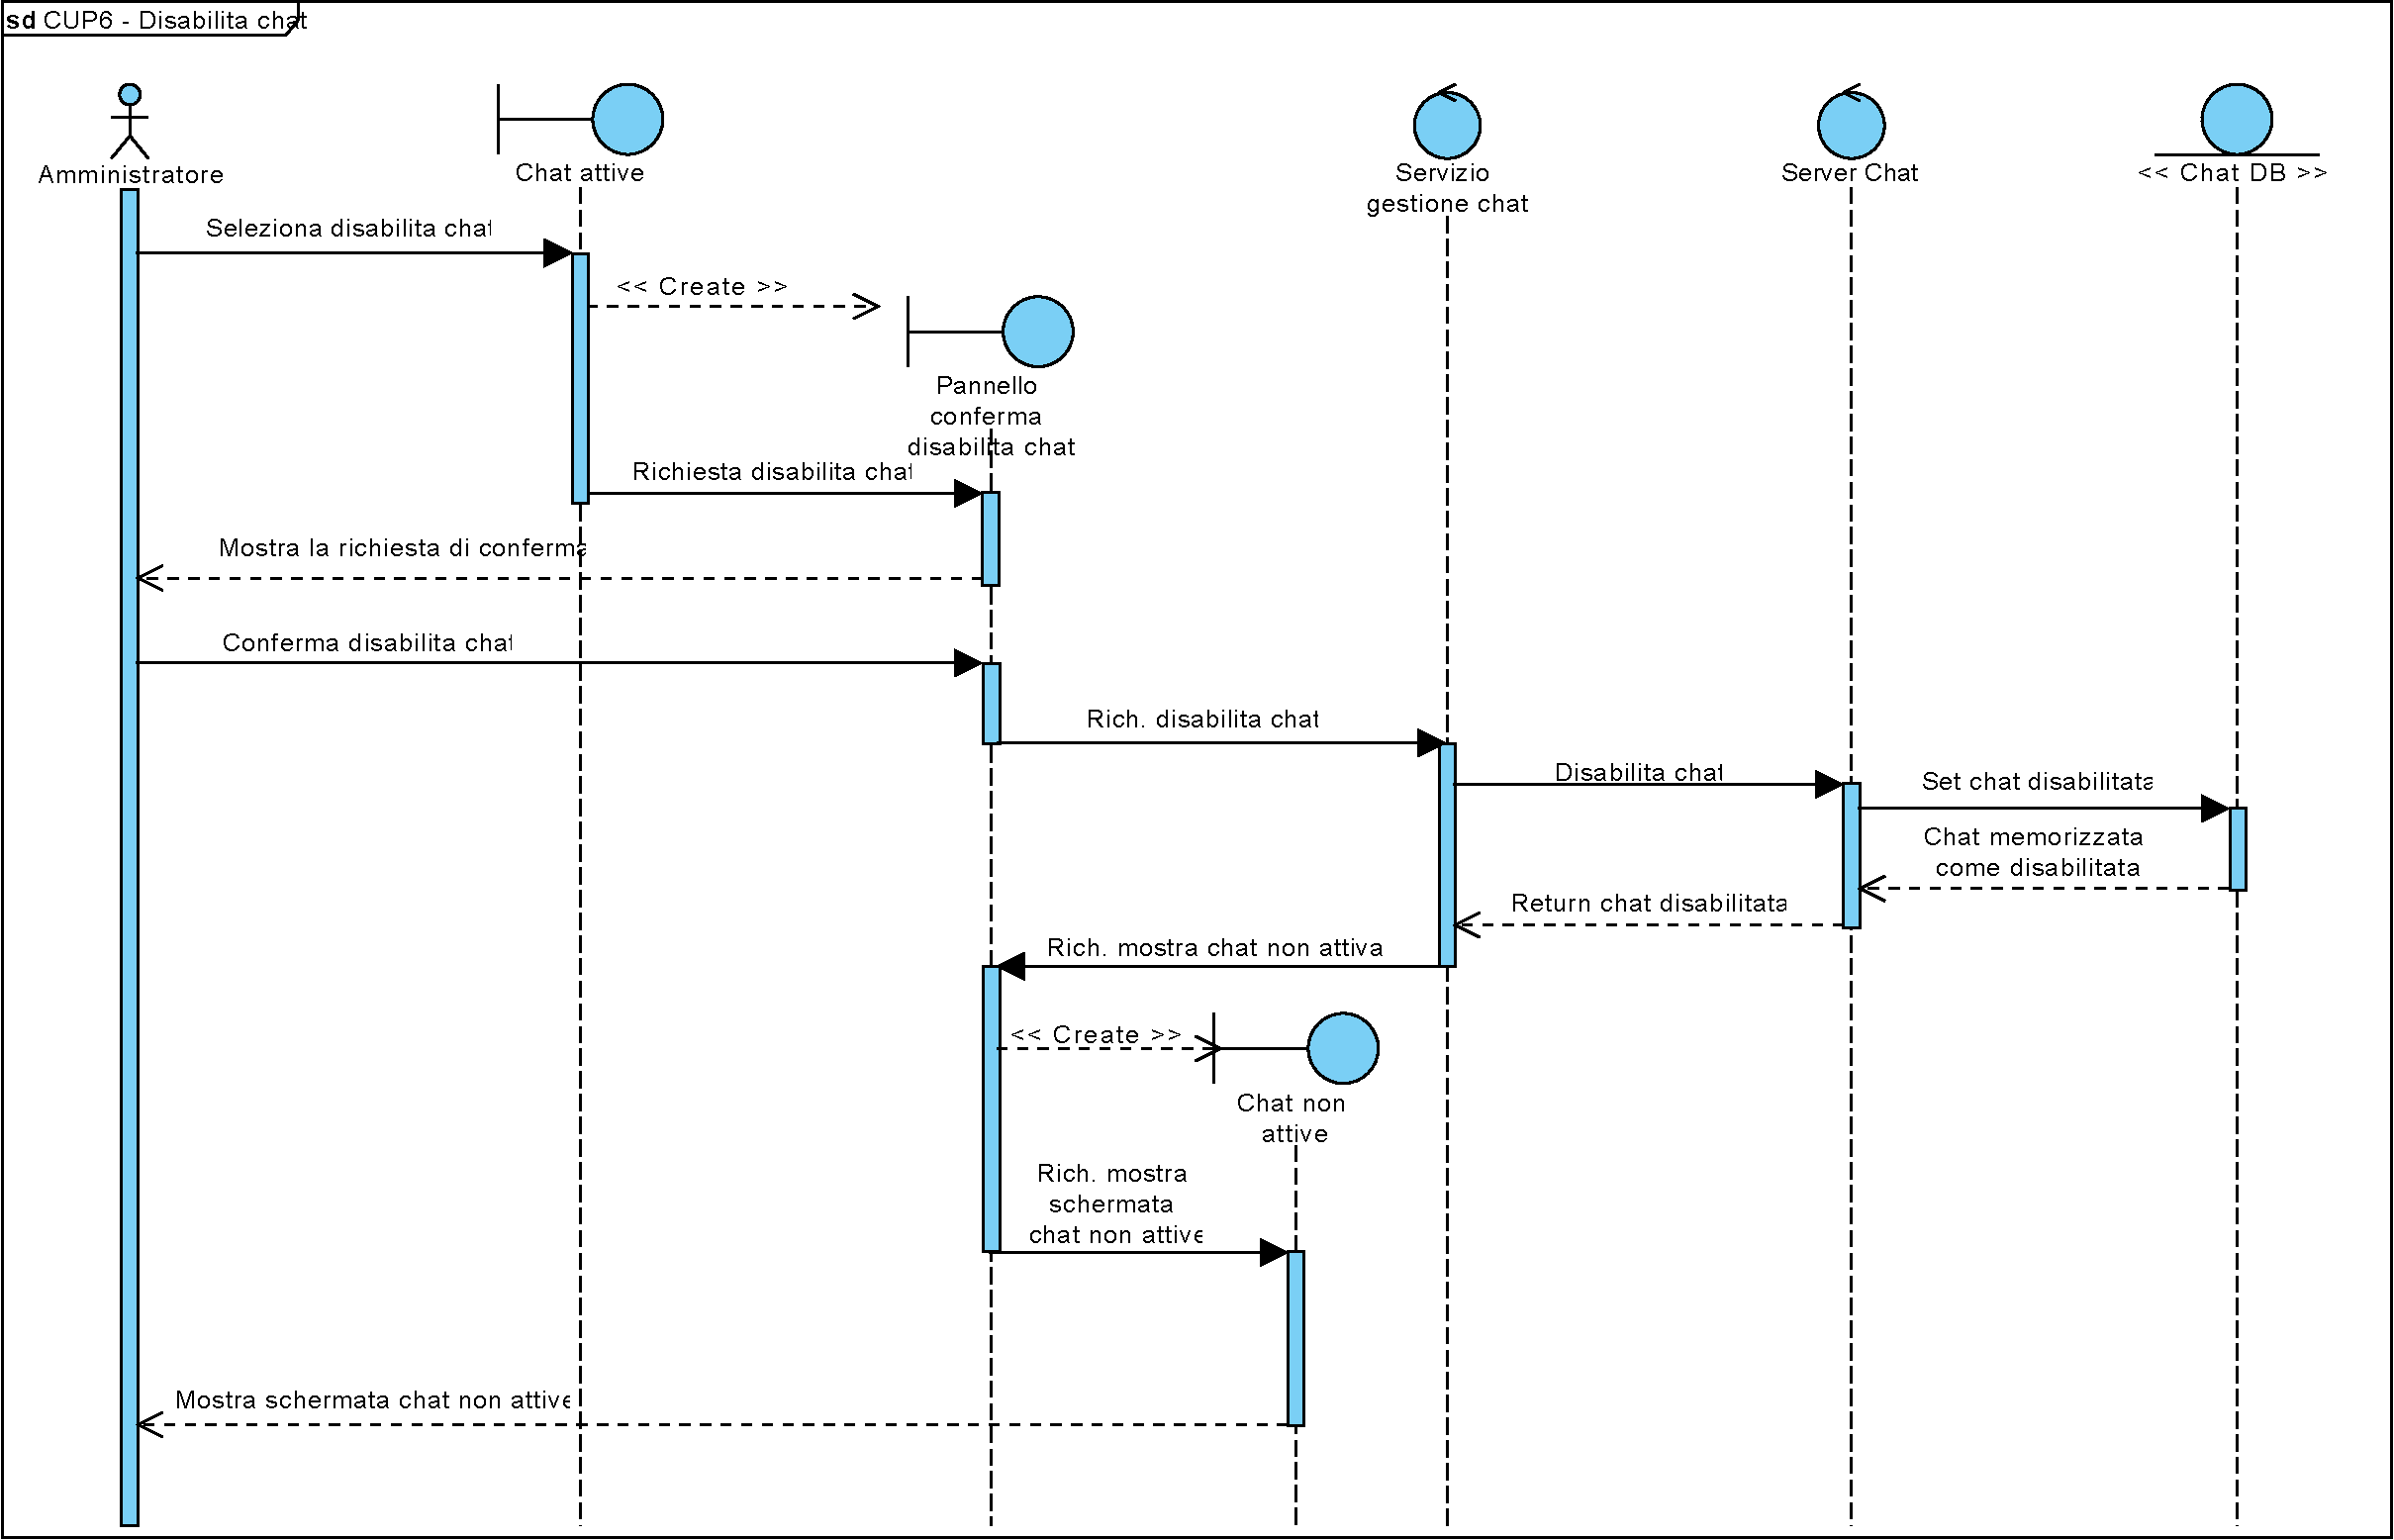
\includegraphics[width=0.9\textwidth]{imgs/gruppo6/sequence/CUP6_disabilita_chat.pdf}
	\caption{CUP6 - Disabilita chat}
	\label{fig:seq-cup6}
\end{figure}

\begin{figure}
	\centering
	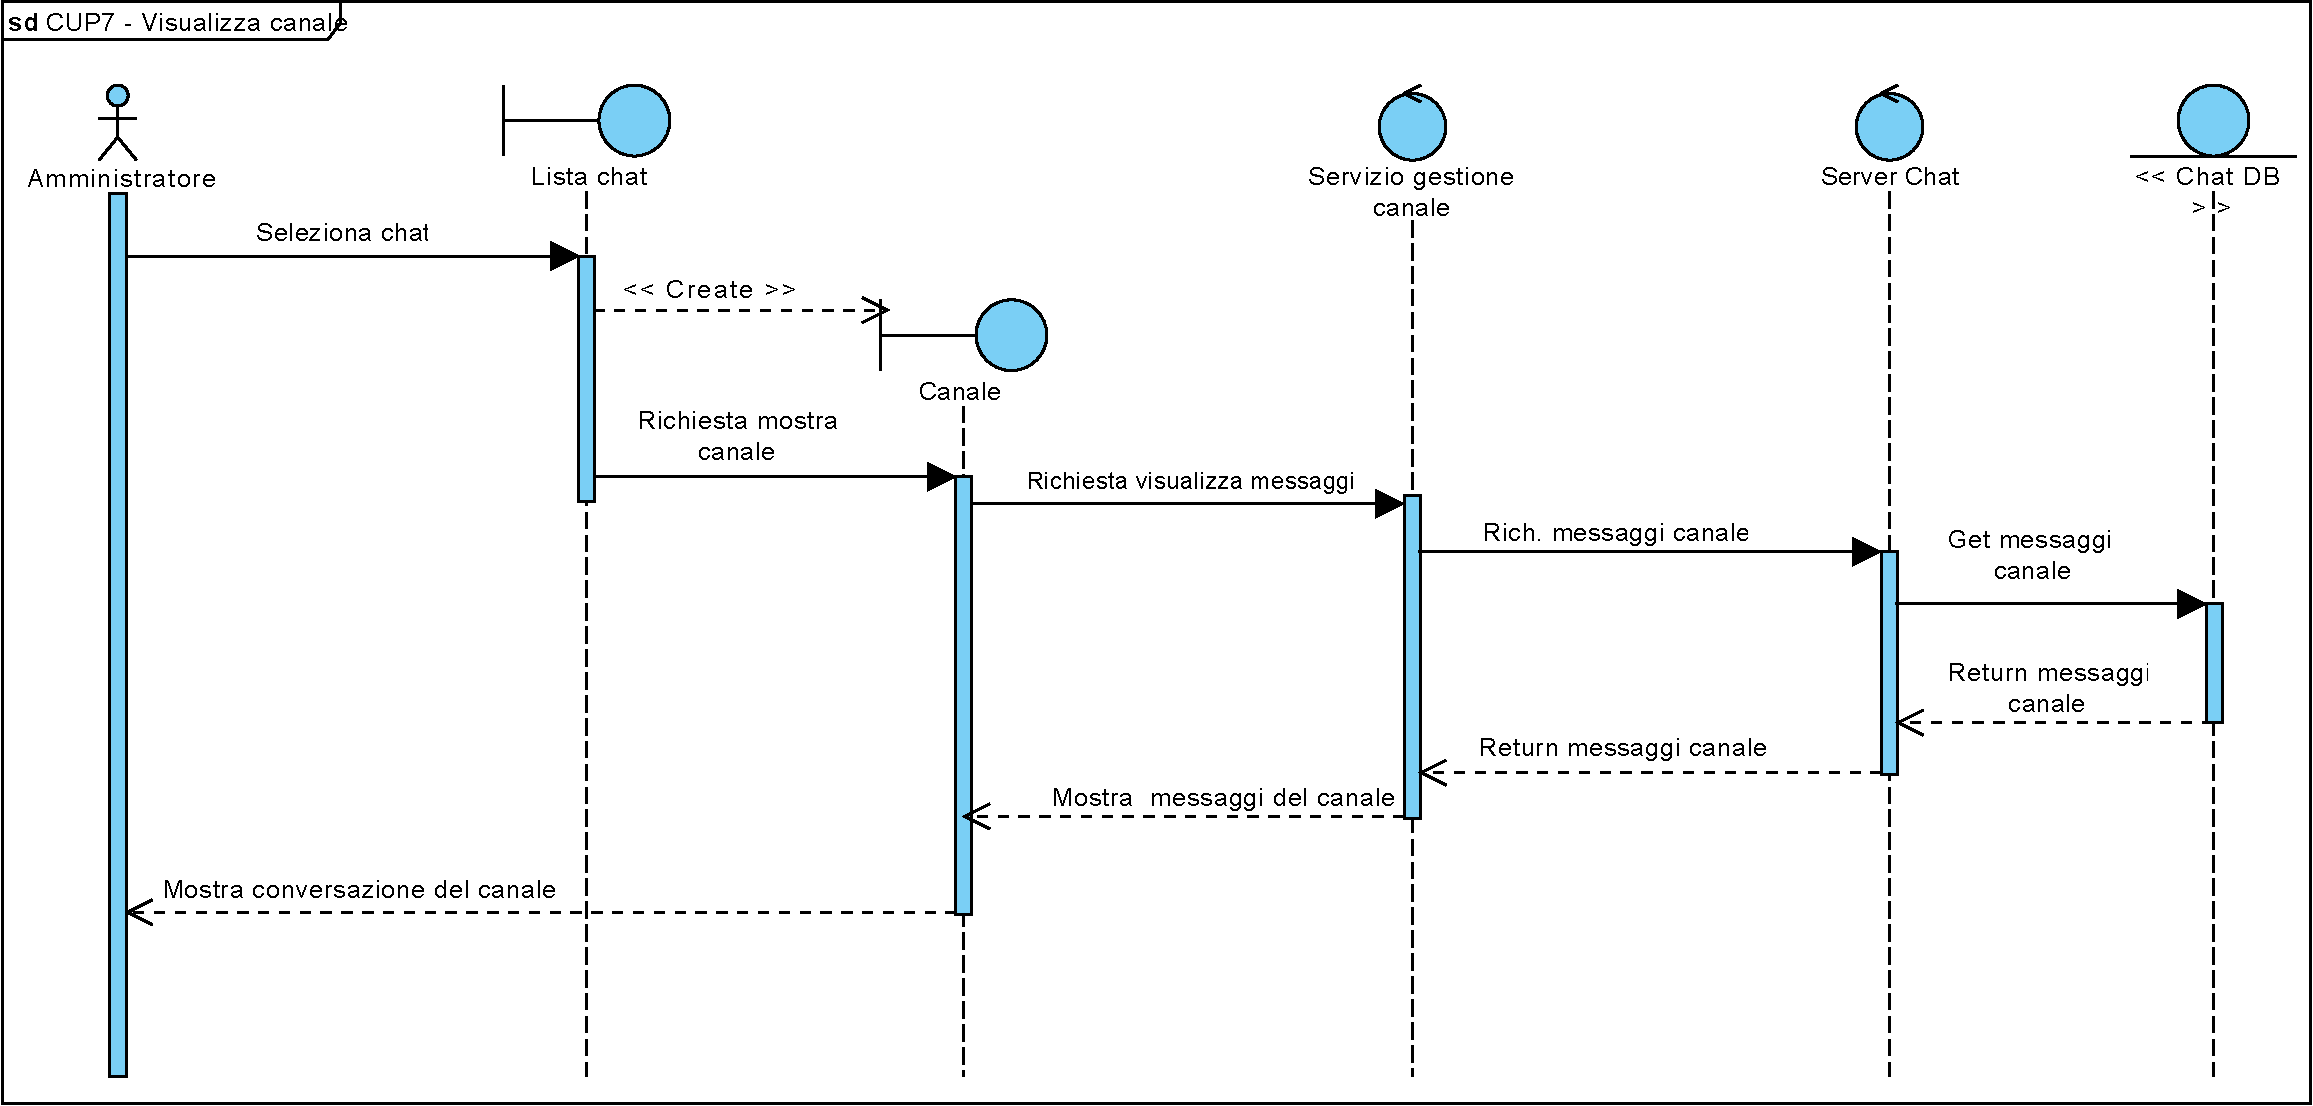
\includegraphics[width=0.9\textwidth]{imgs/gruppo6/sequence/CUP7_visualizza_canale.pdf}
	\caption{CUP7 - Visualizza canale}
	\label{fig:seq-cup7}
\end{figure}

\begin{figure}
	\centering
	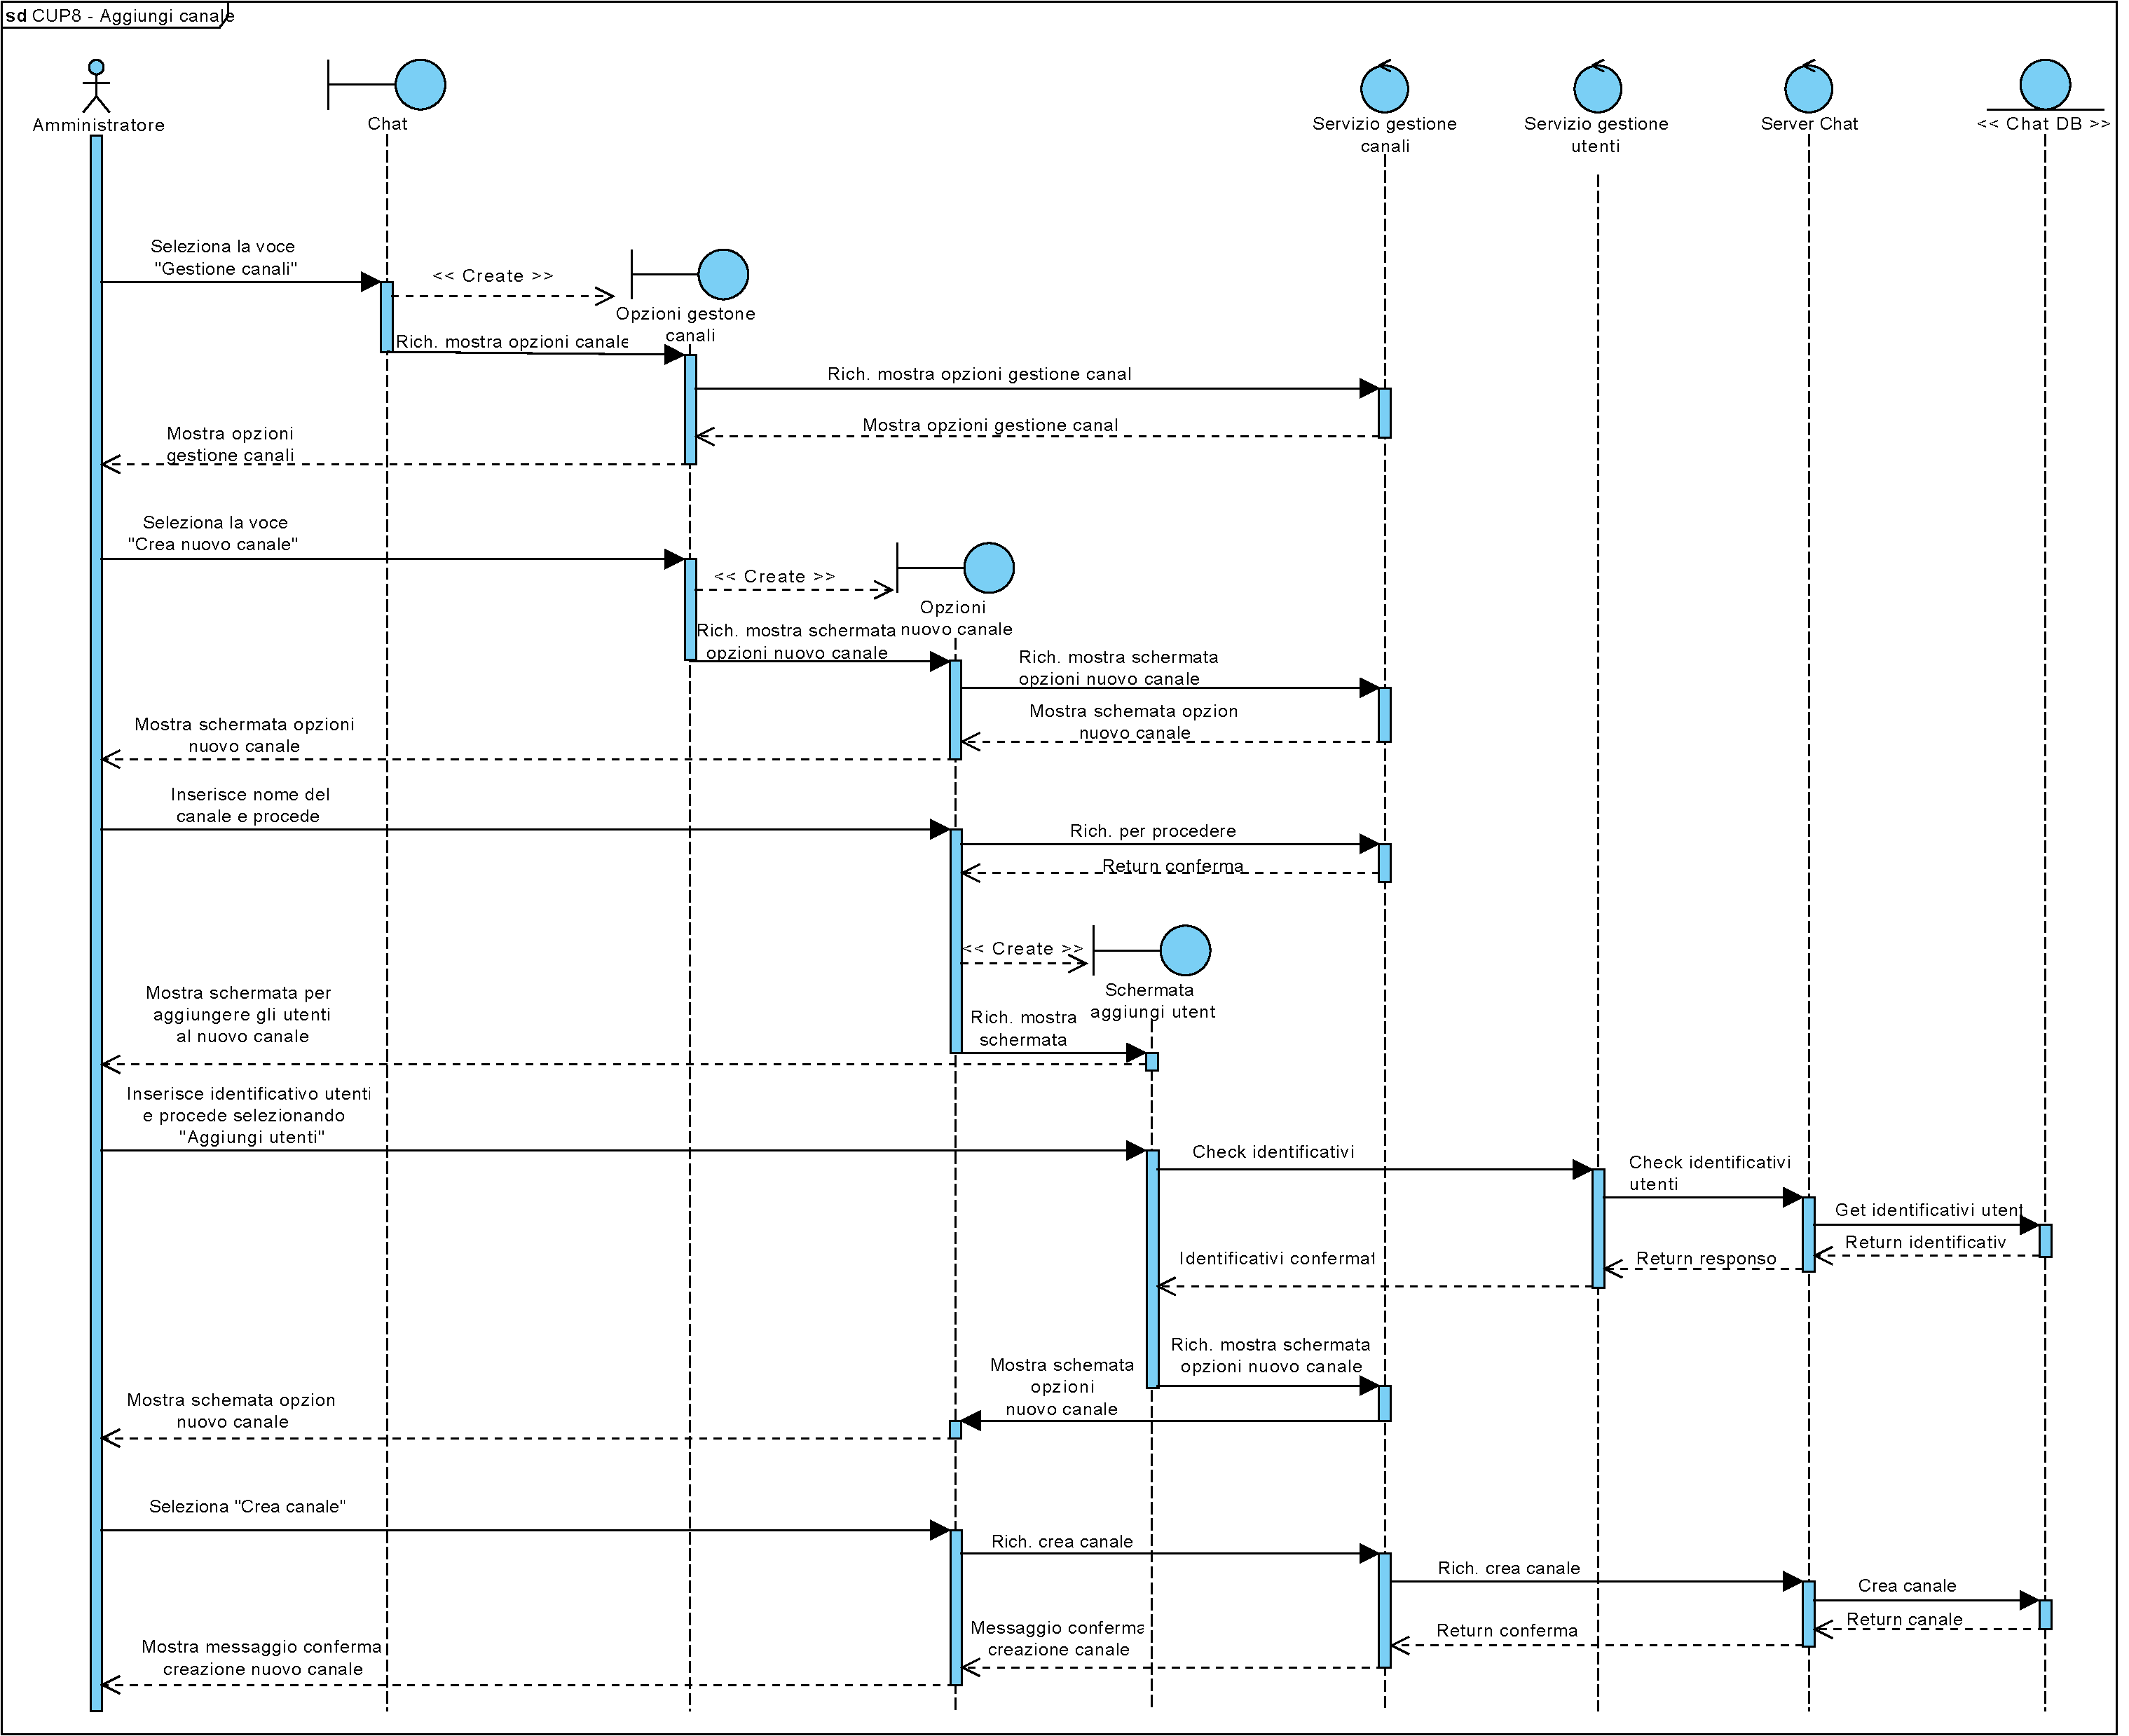
\includegraphics[width=0.9\textwidth]{imgs/gruppo6/sequence/CUP8_aggiungi_canale.pdf}
	\caption{CUP8 - Aggiungi canale}
	\label{fig:seq-cup8}
\end{figure}

\begin{figure}
	\centering
	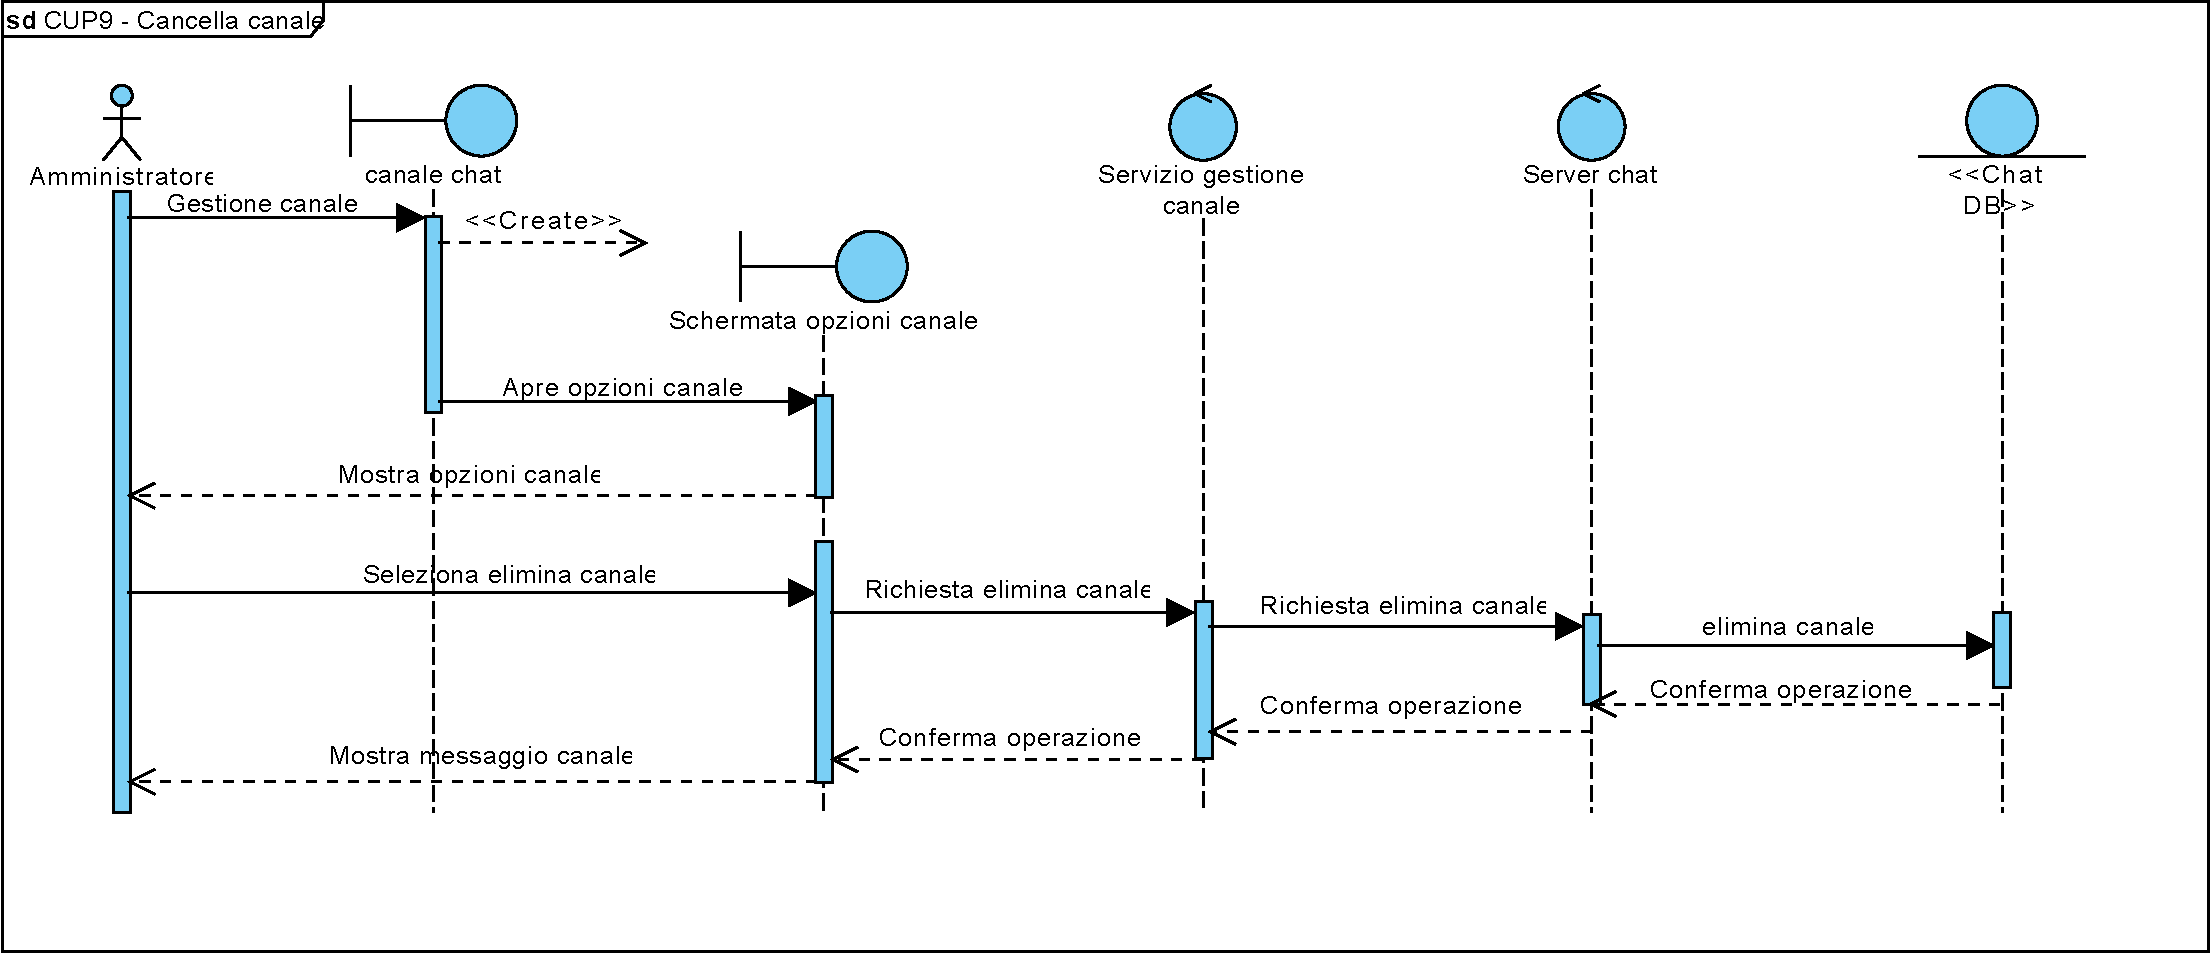
\includegraphics[width=0.9\textwidth]{imgs/gruppo6/sequence/CUP9_cancella_canale.pdf}
	\caption{CUP9 - Cancella canale}
	\label{fig:seq-cup9}
\end{figure}

\begin{figure}
	\centering
	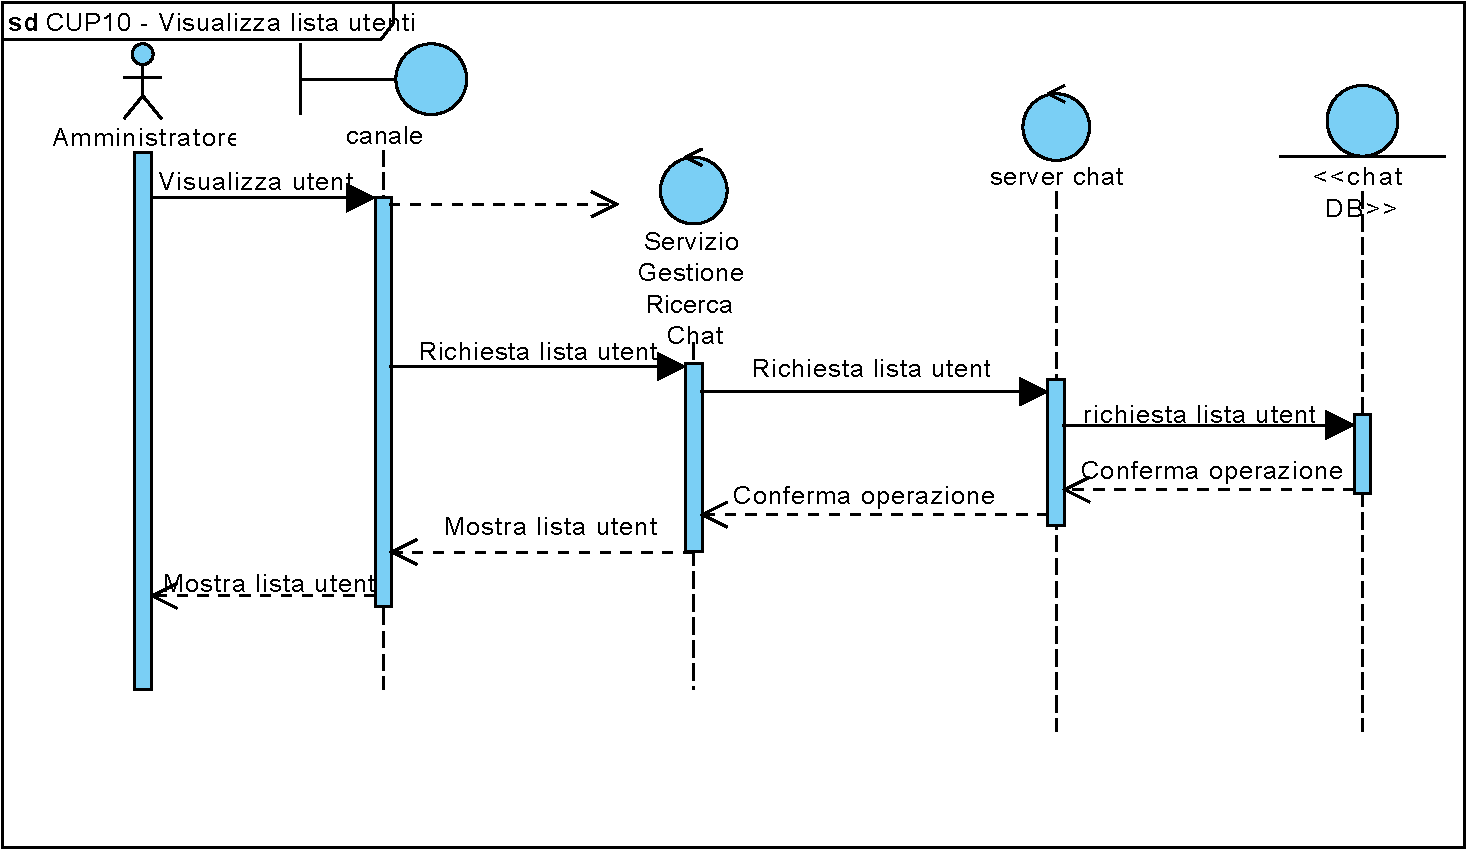
\includegraphics[width=0.9\textwidth]{imgs/gruppo6/sequence/CUP10_visualizza_lista_utenti.pdf}
	\caption{CUP10 - Visualizza lista utenti}
	\label{fig:seq-cup10}
\end{figure}

\begin{figure}
	\centering
	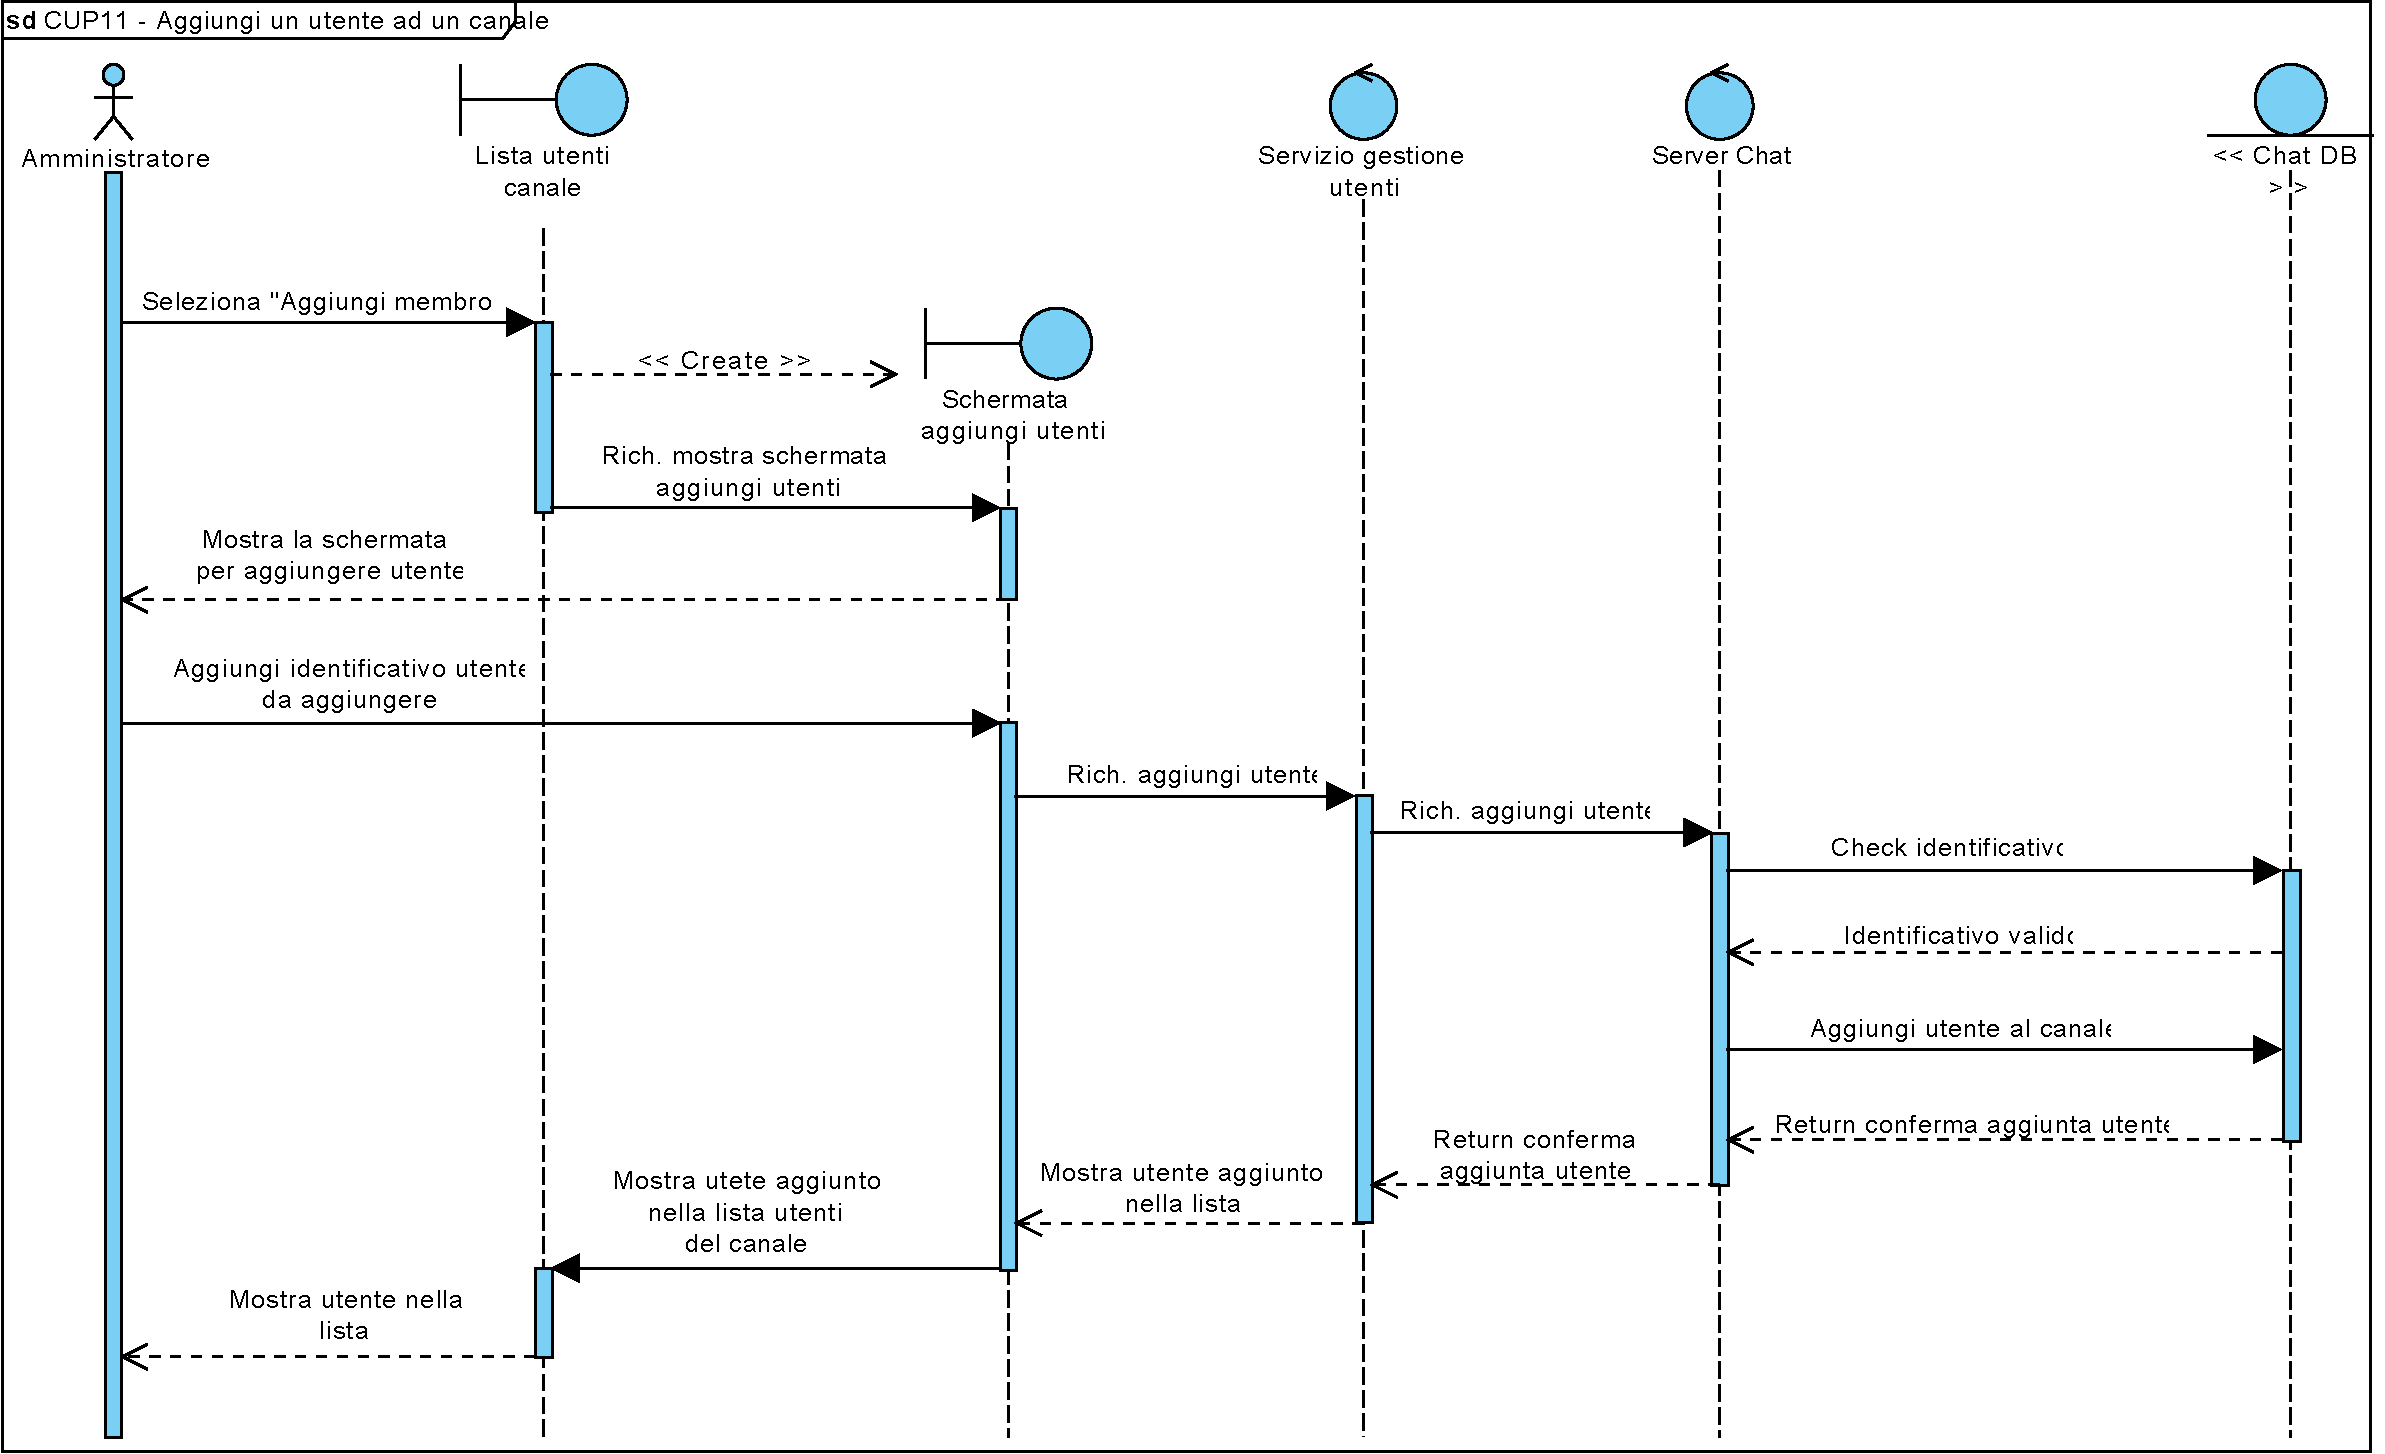
\includegraphics[width=0.9\textwidth]{imgs/gruppo6/sequence/CUP11_aggiungi_un_utente_ad_un_canale.pdf}
	\caption{CUP11 - Aggiungi un utente ad un canale}
	\label{fig:seq-cup11}
\end{figure}

\begin{figure}
	\centering
	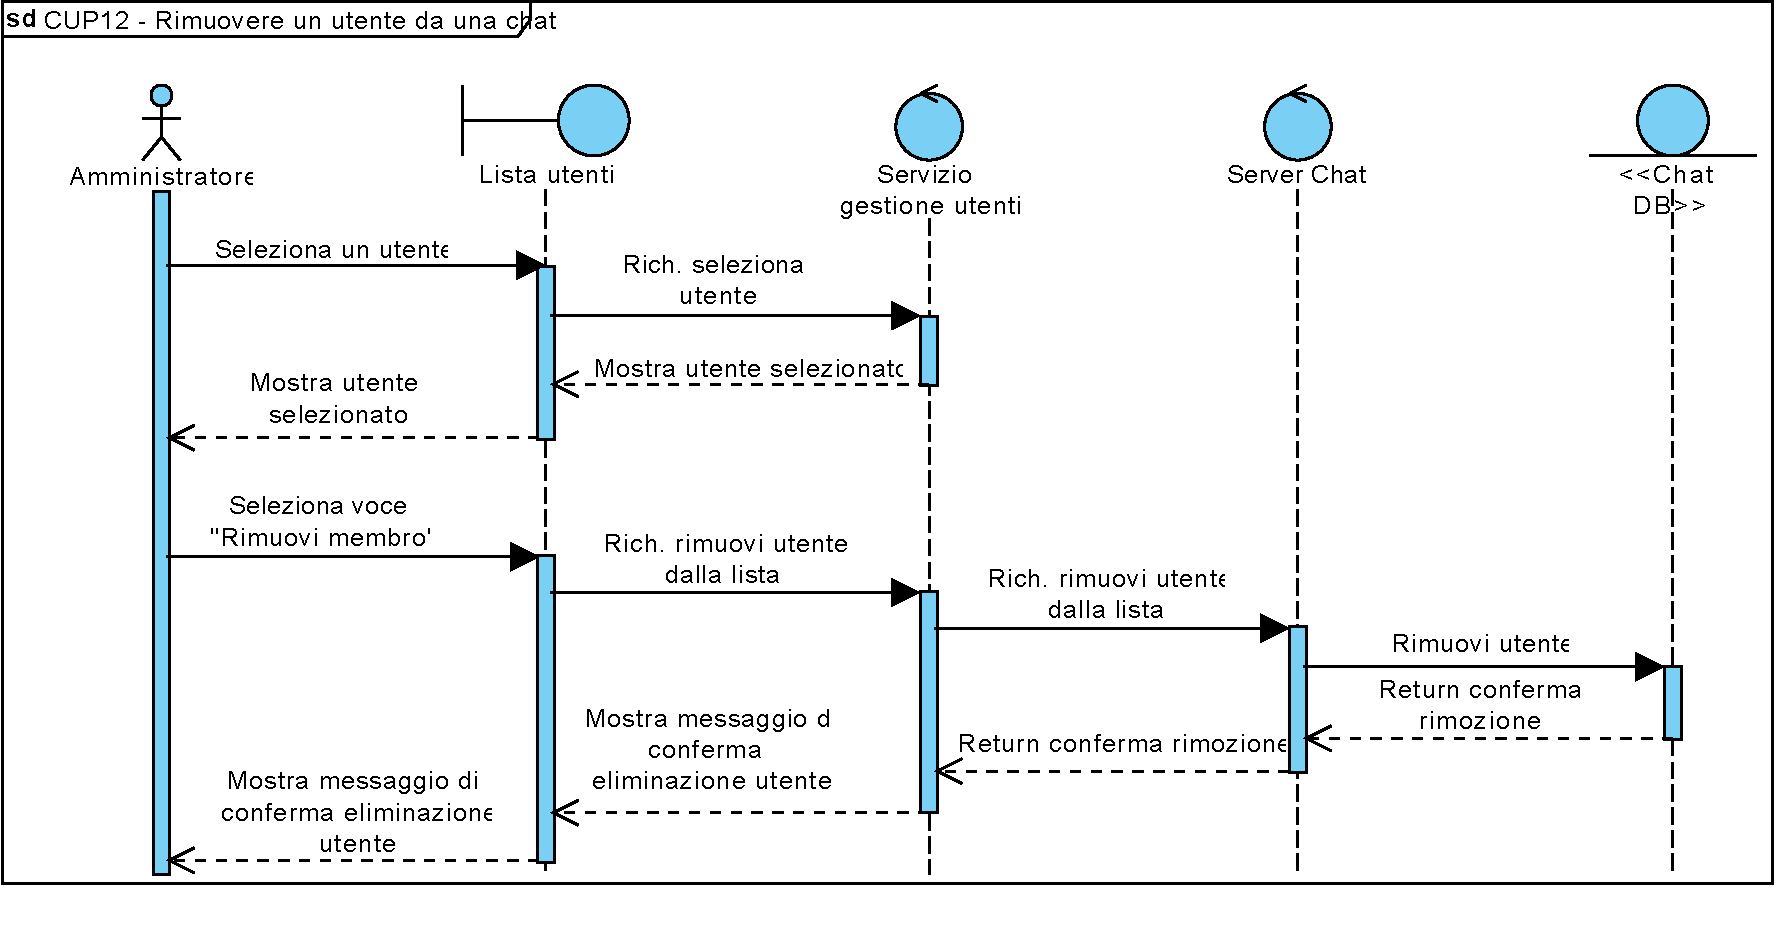
\includegraphics[width=0.9\textwidth]{imgs/gruppo6/sequence/CUP12_rimuovere_un_utente_da_un_canale.pdf}
	\caption{CUP12 - Rimuovere un utente ad un canale}
	\label{fig:seq-cup12}
\end{figure}

\begin{figure}
	\centering
	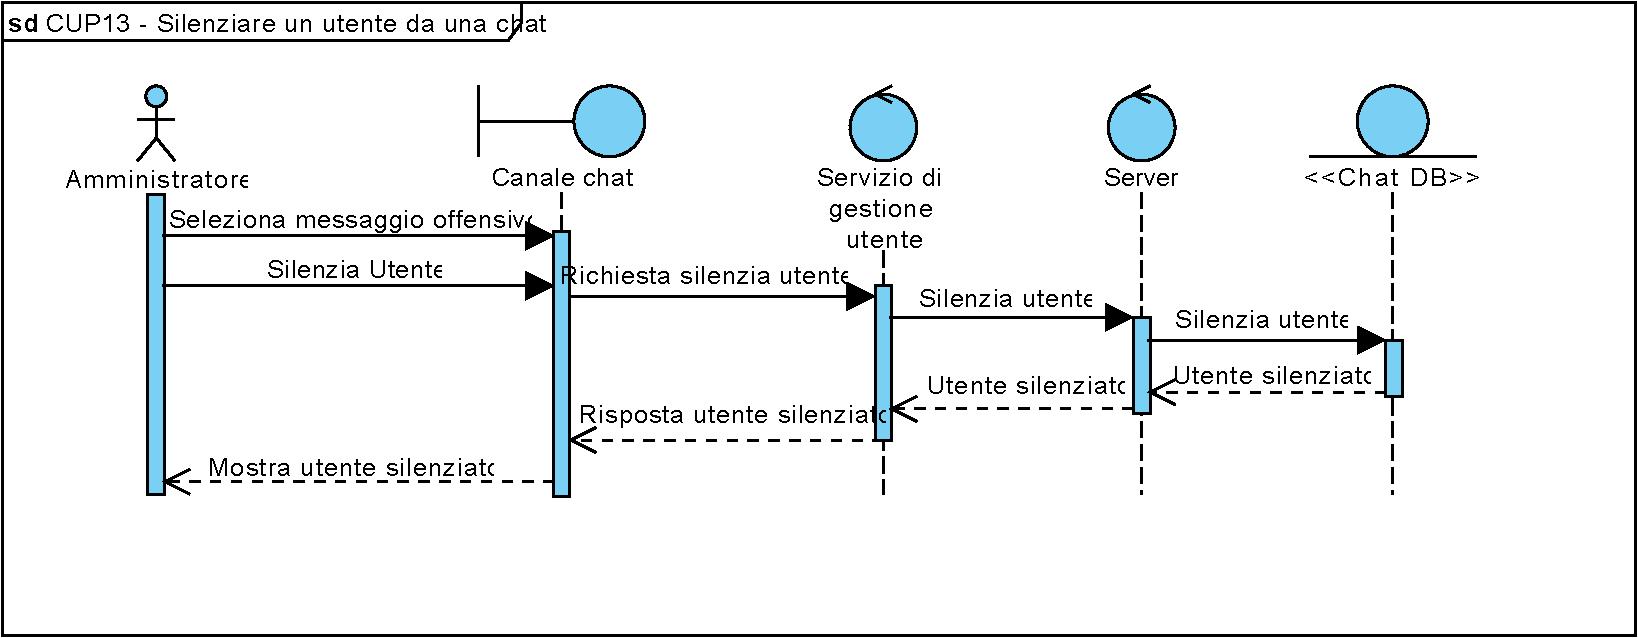
\includegraphics[width=0.9\textwidth]{imgs/gruppo6/sequence/CUP13_silenzia_un_utente_da_una_chat.pdf}
	\caption{CUP13 - Silenzia un utente da una chat}
	\label{fig:seq-cup13}
\end{figure}

\begin{figure}
	\centering
	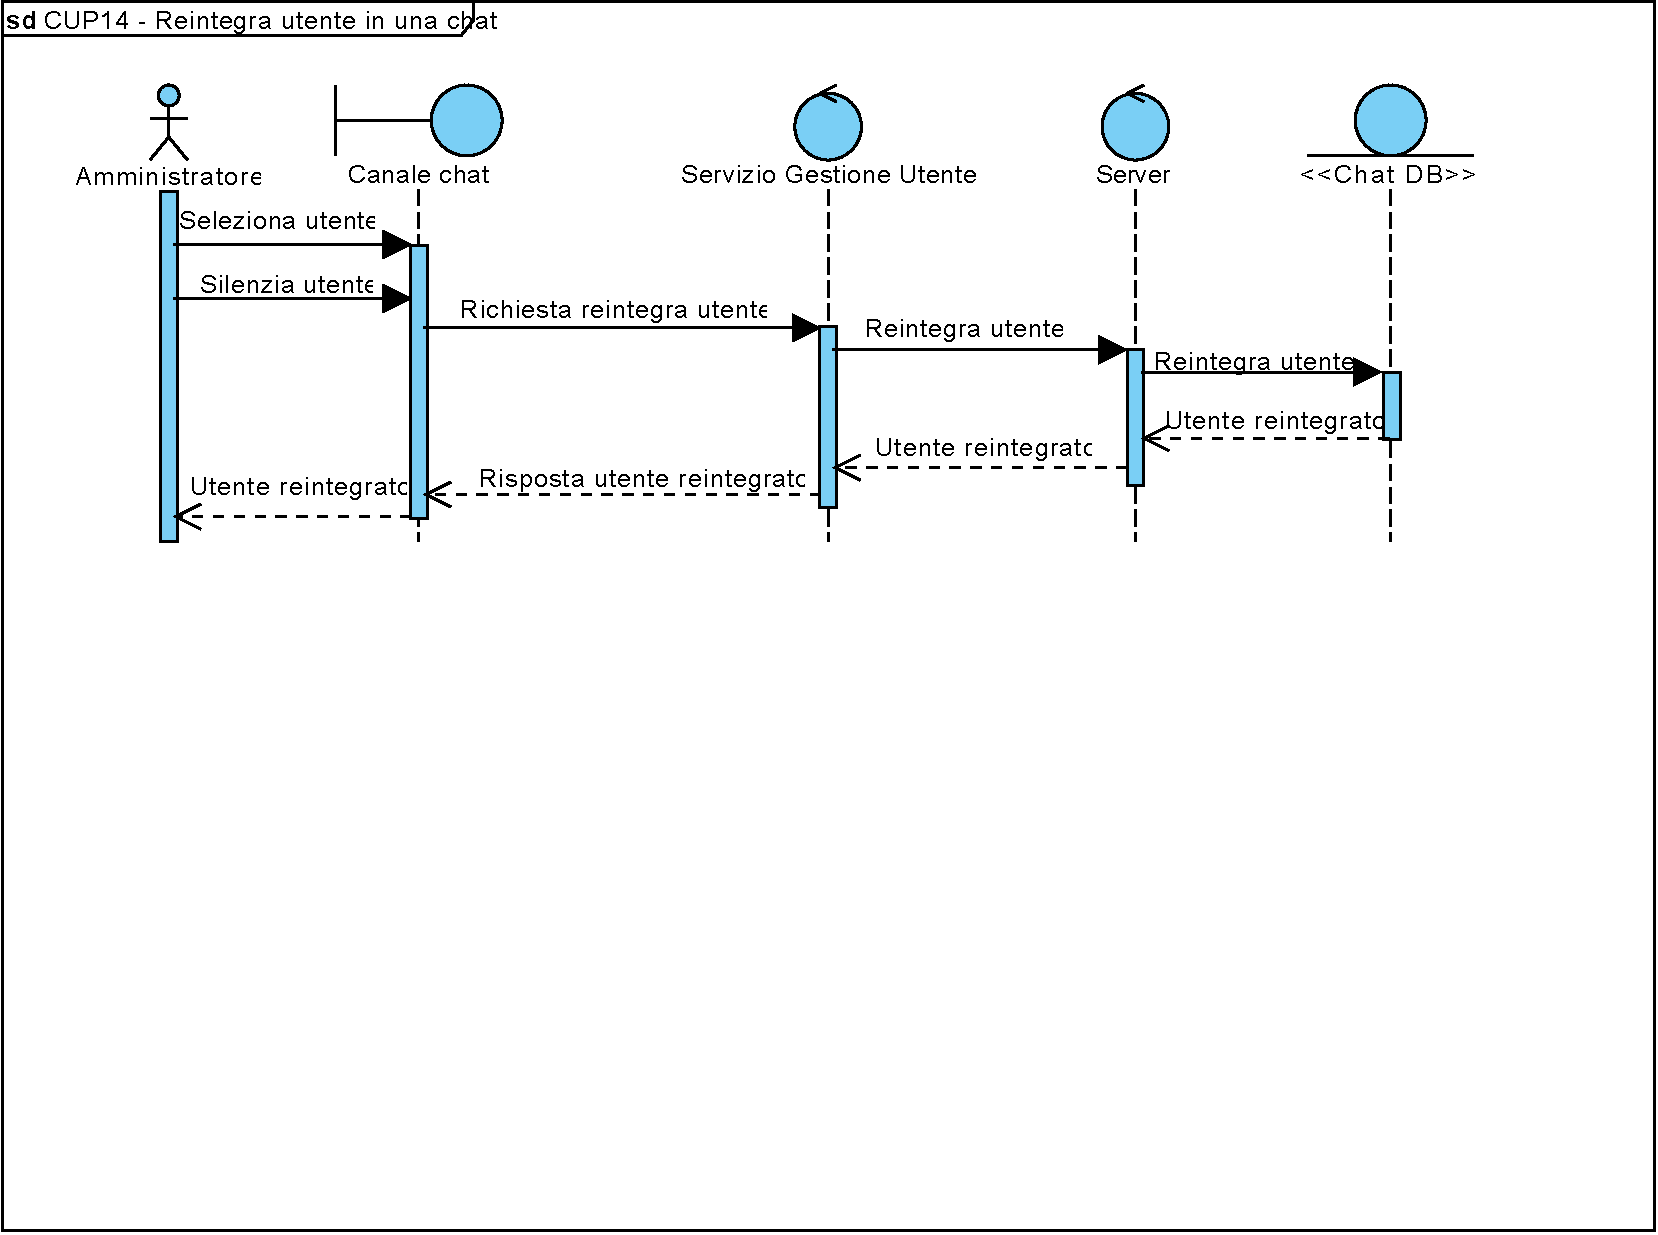
\includegraphics[width=0.9\textwidth]{imgs/gruppo6/sequence/CUP14_reintegra_utente_in_una_chat.pdf}
	\caption{CUP14 - Reintegra utente in una chat}
	\label{fig:seq-cup14}
\end{figure}

\begin{figure}
	\centering
	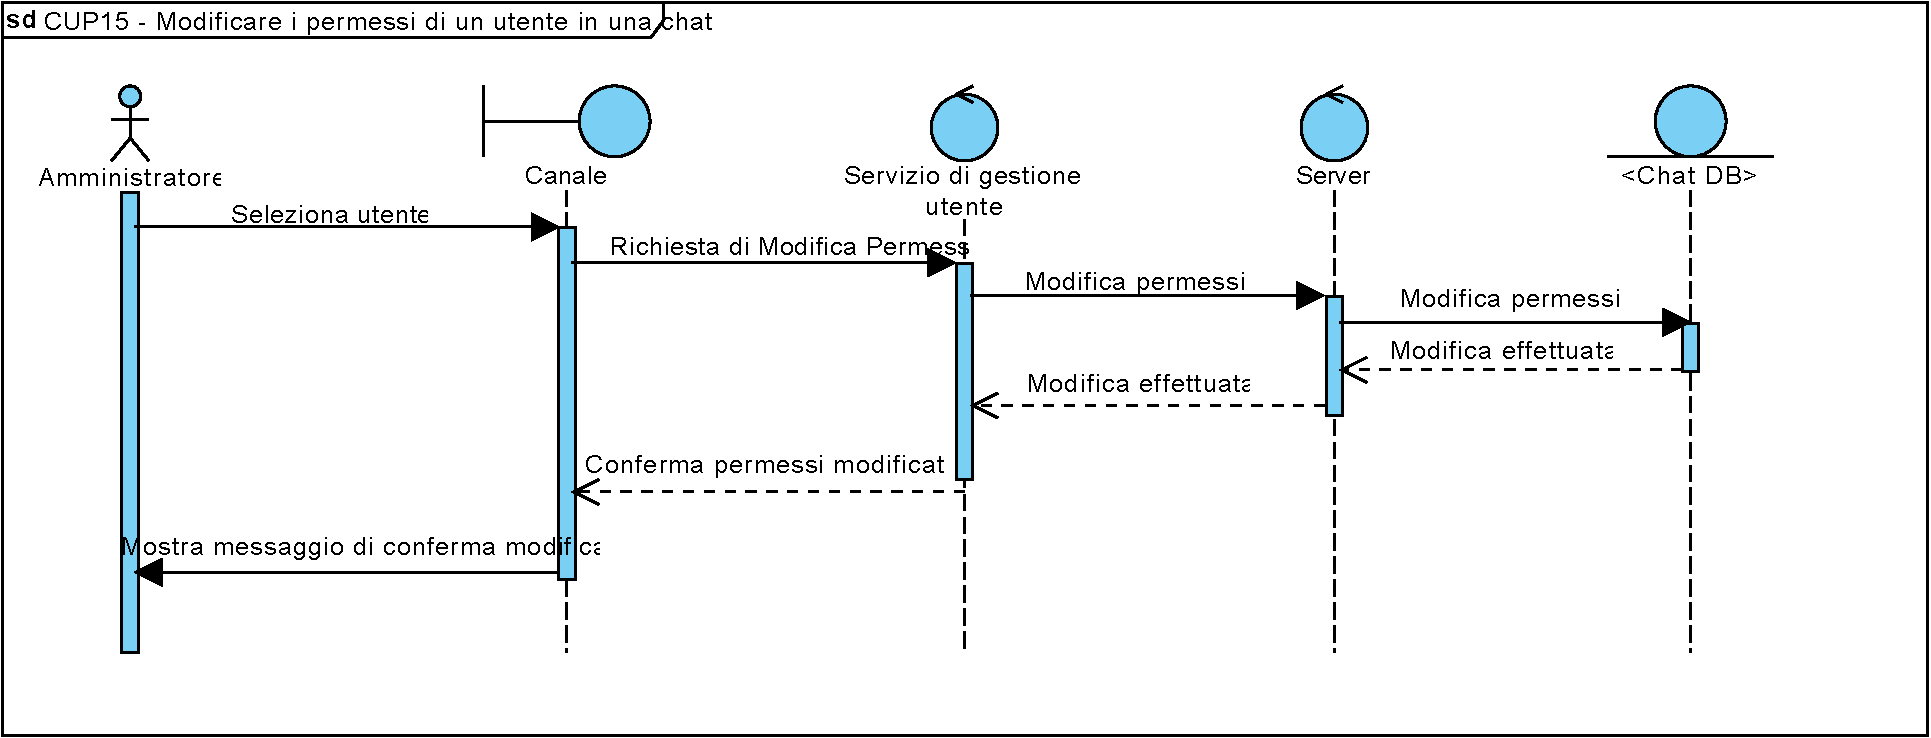
\includegraphics[width=0.9\textwidth]{imgs/gruppo6/sequence/CUP15_modificare_i_permessi_di_un_utente.pdf}
	\caption{CUP15 - Modificare i permessi di un utente}
	\label{fig:seq-cup15}
\end{figure}

\begin{figure}
	\centering
	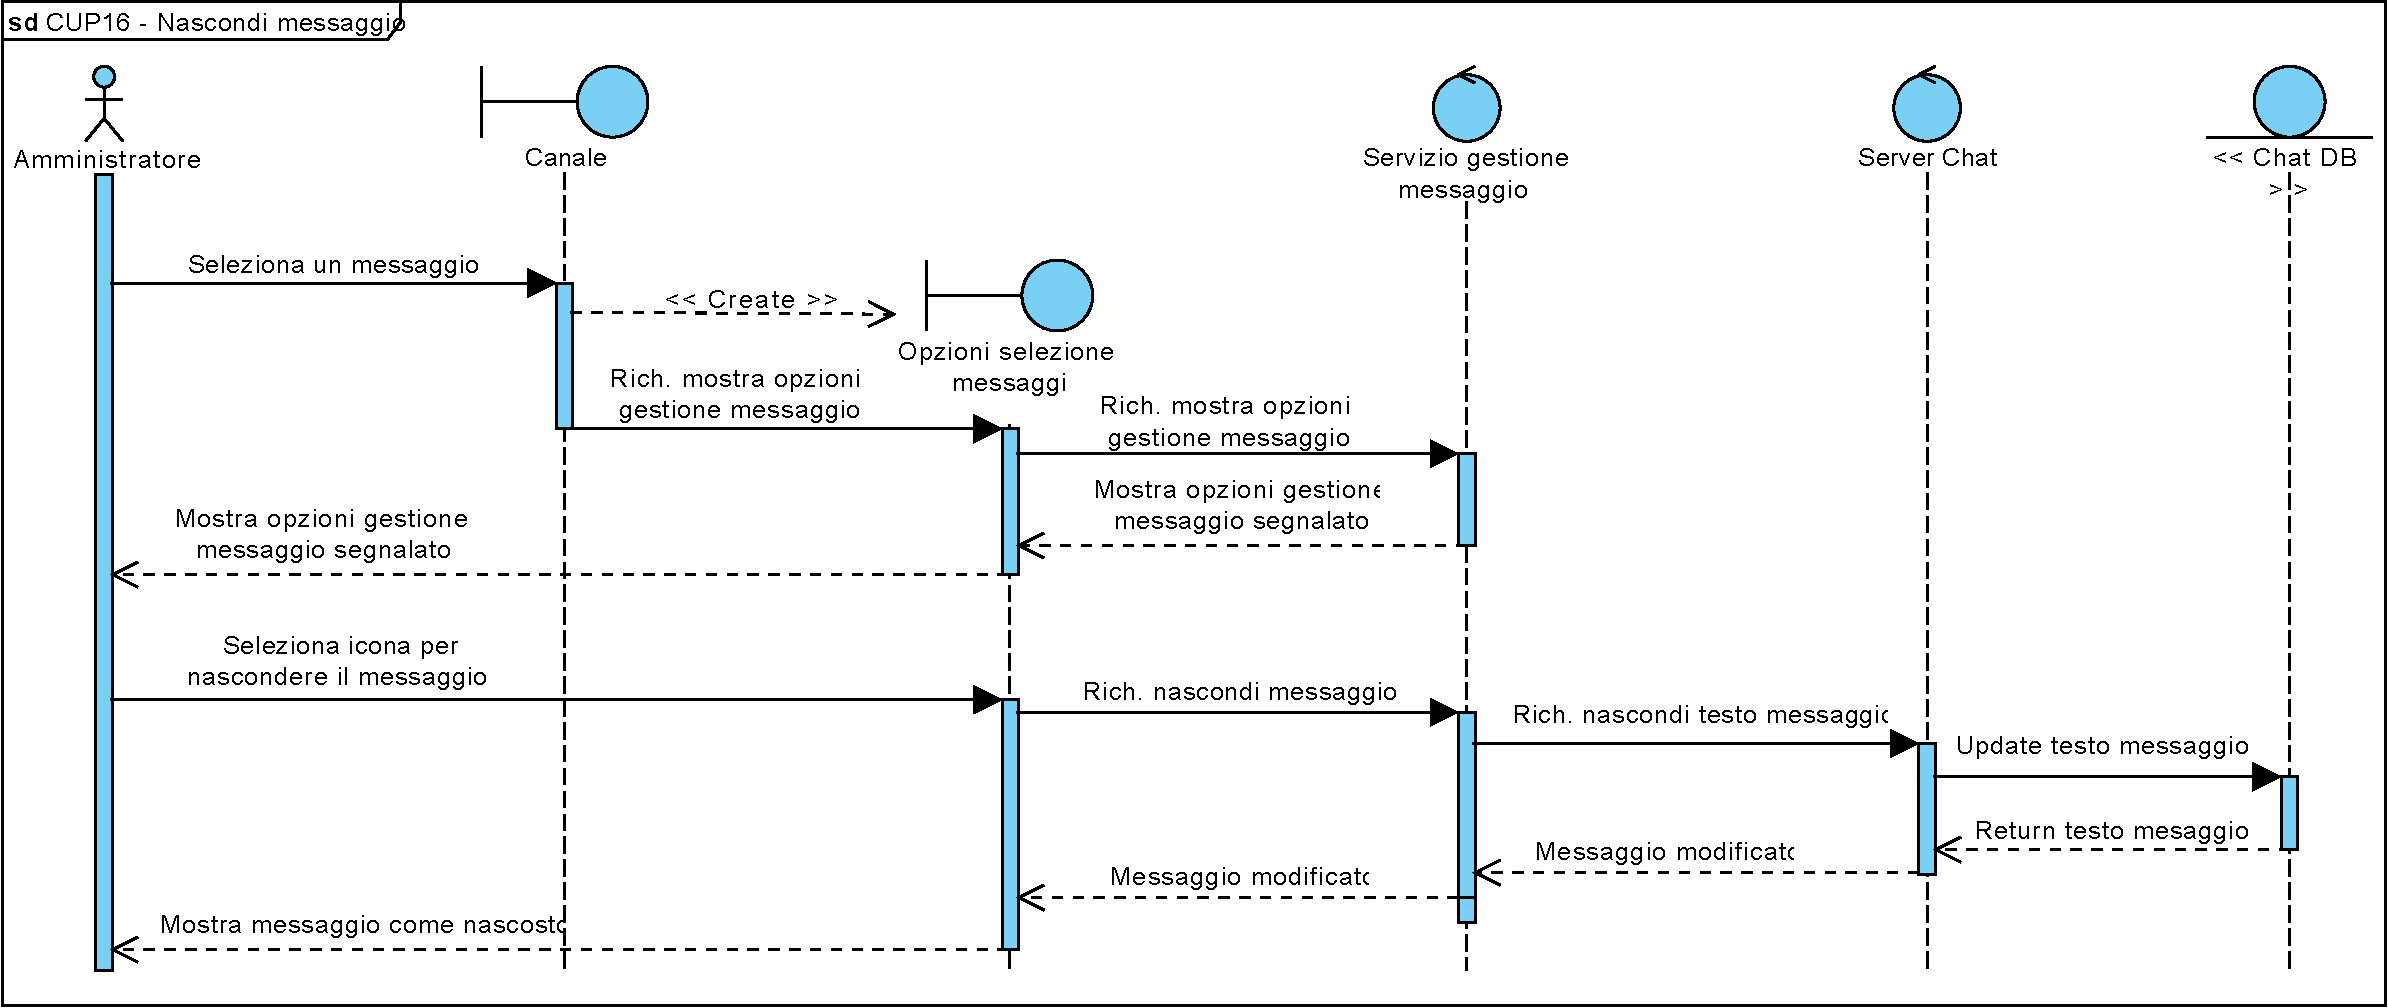
\includegraphics[width=0.9\textwidth]{imgs/gruppo6/sequence/CUP16_nascondi_messaggio.pdf}
	\caption{CUP16 - Nascondi messaggio}
	\label{fig:seq-cup16}
\end{figure}

\begin{figure}
	\centering
	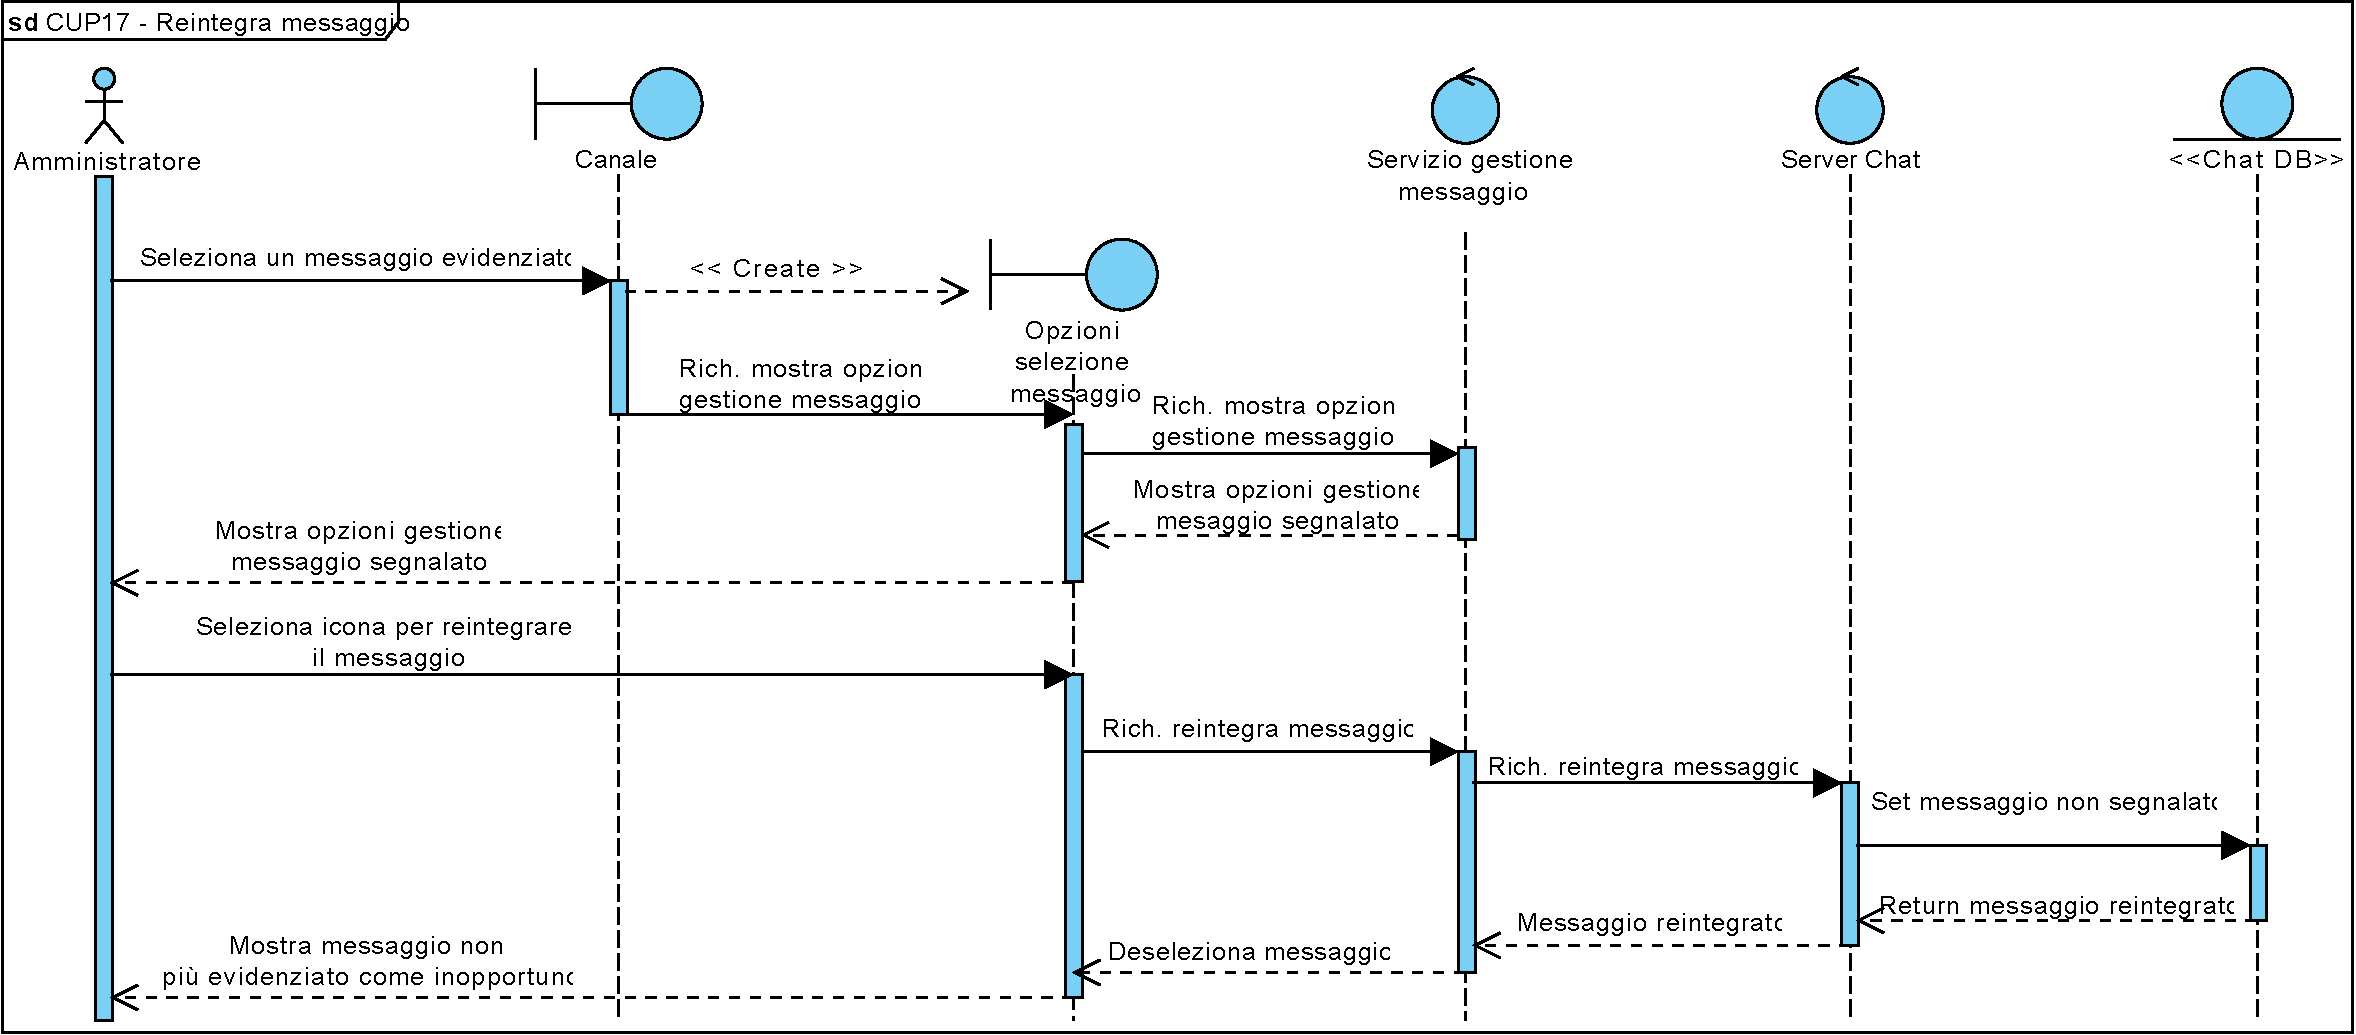
\includegraphics[width=0.9\textwidth]{imgs/gruppo6/sequence/seq_cup17_reintegra_messaggio.pdf}
	\caption{CUP17 - Reintegra messaggio}
	\label{fig:seq-cup17}
\end{figure}

\begin{figure}
	\centering
	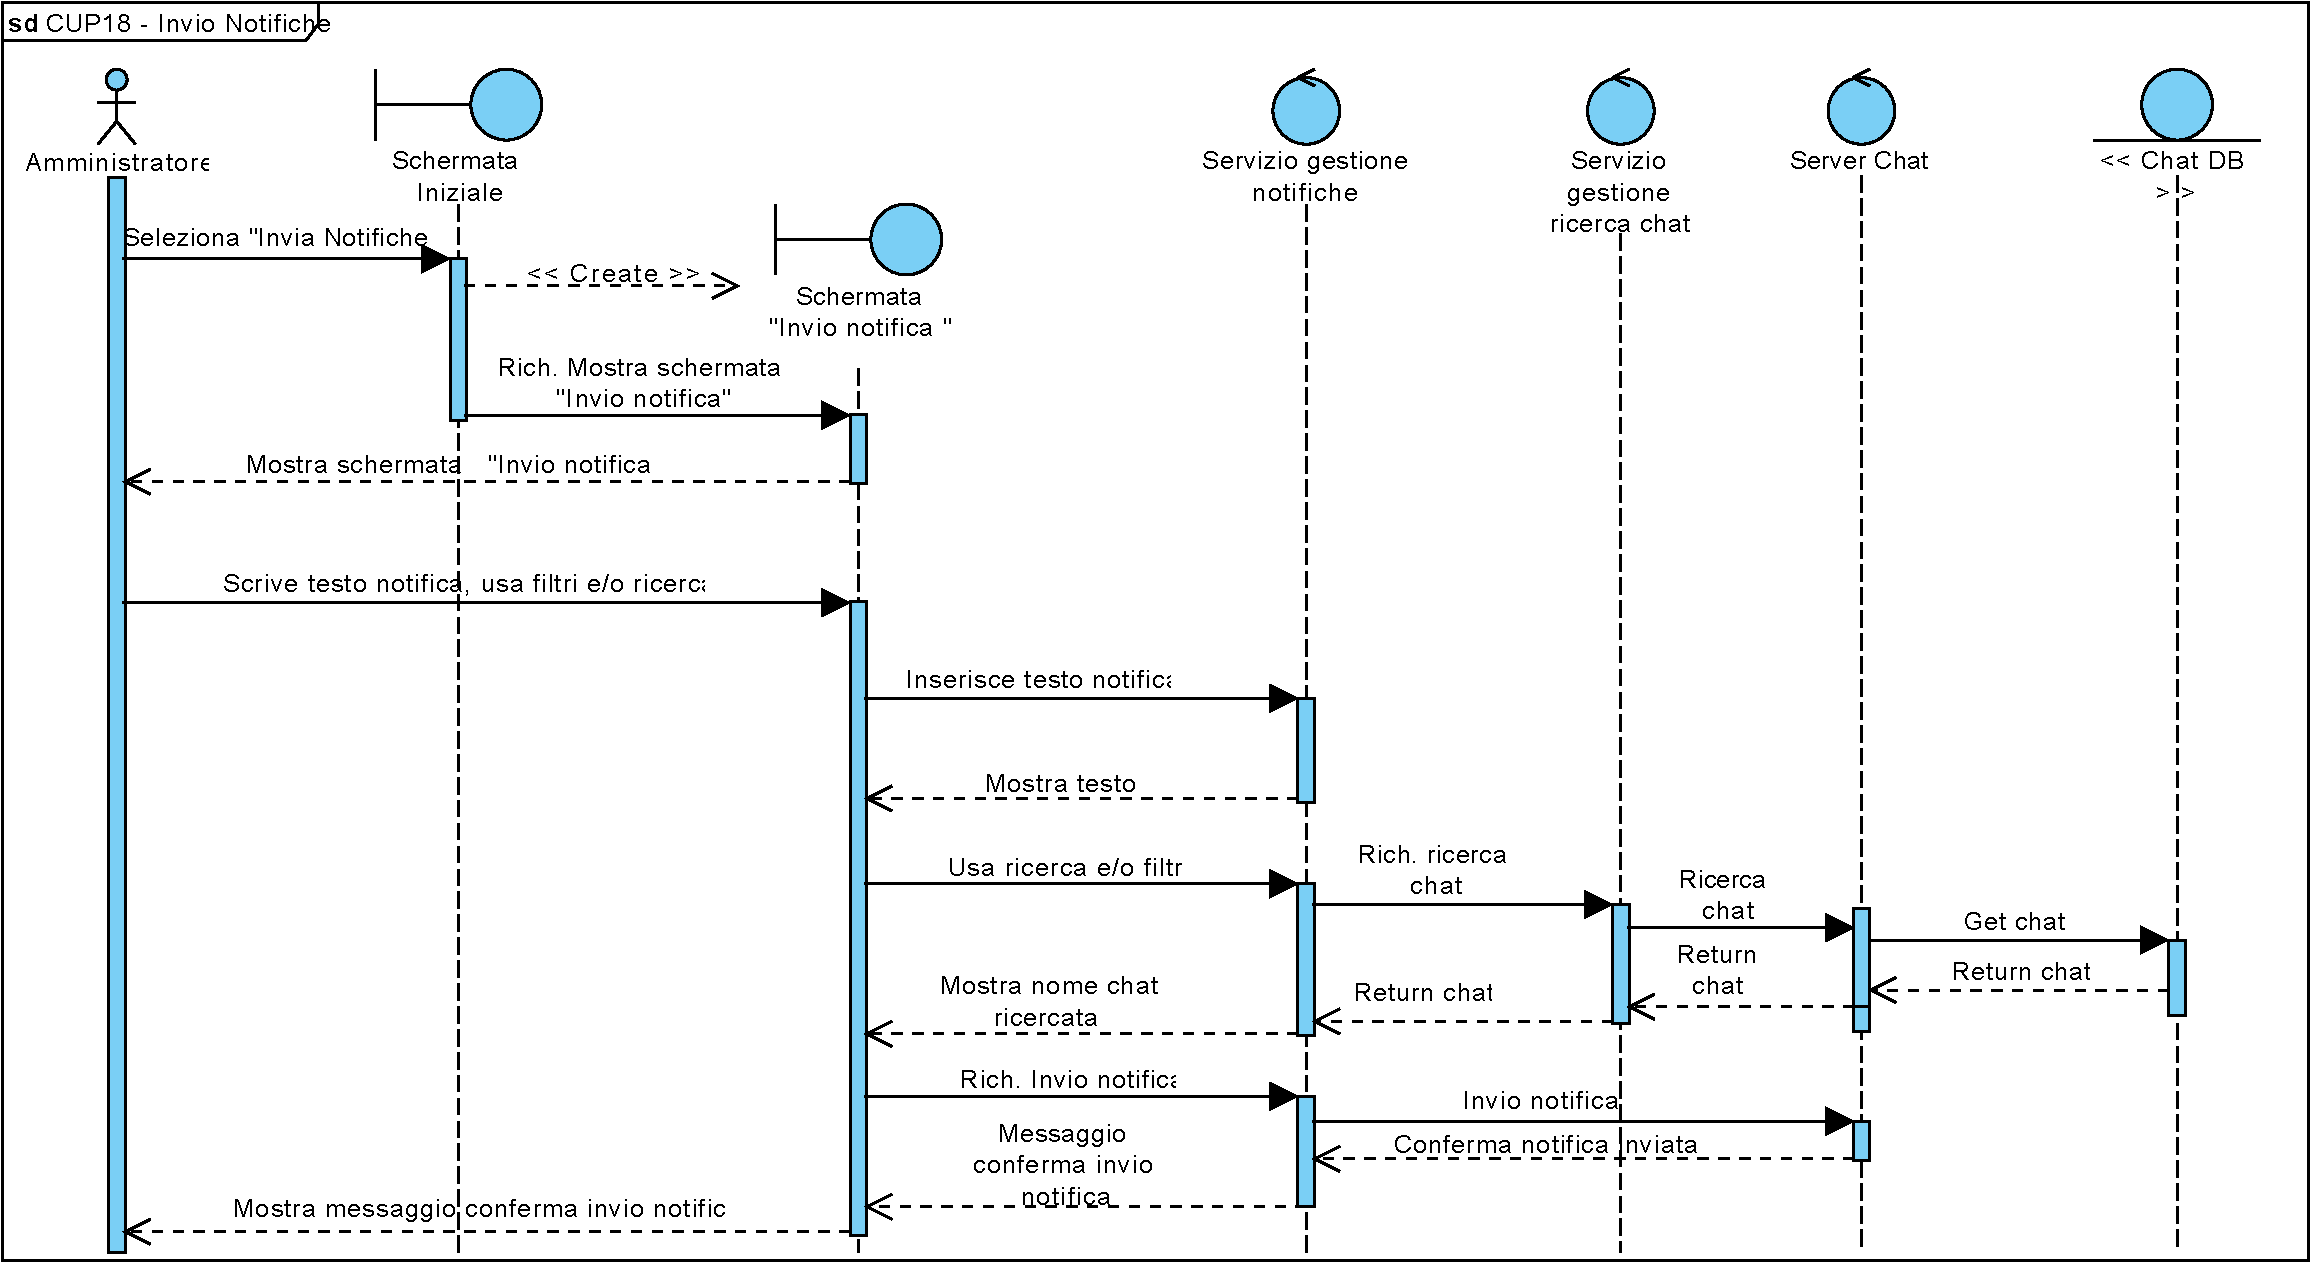
\includegraphics[width=0.9\textwidth]{imgs/gruppo6/sequence/CUP18_invio_notifica.pdf}
	\caption{CUP18 - Invio notifica}
	\label{fig:seq-cup18}
\end{figure}


\begin{figure}
	\centering
	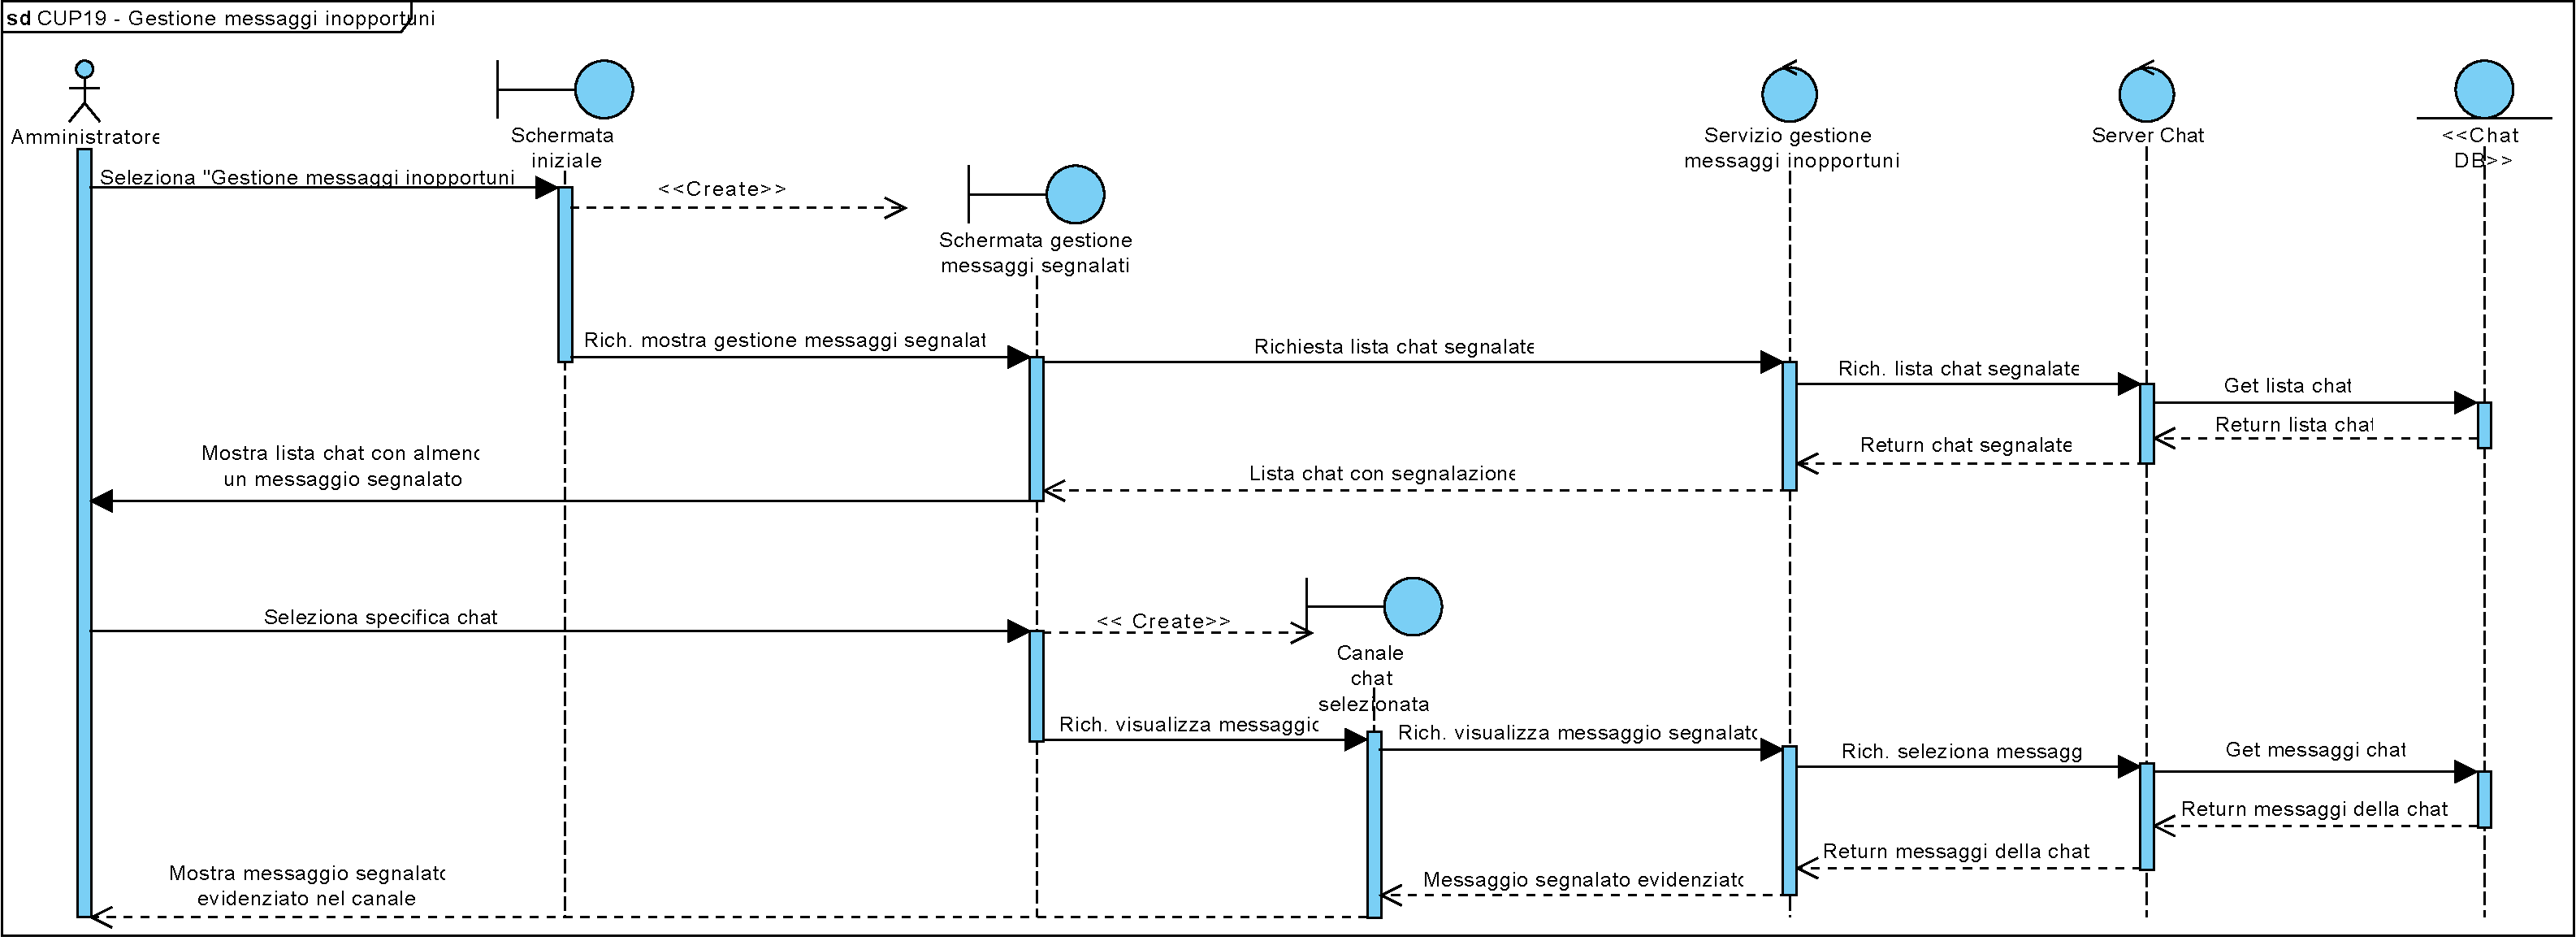
\includegraphics[width=0.9\textwidth]{imgs/gruppo6/sequence/CUP19_gestione_messaggi_inopportuni.pdf}
	\caption{CUP19 - Gestione messaggi inopportuni}
	\label{fig:seq-cup19}
\end{figure}

\pagebreak

\begin{figure}[!h]
	\subsection{Eccezioni}
	\centering
	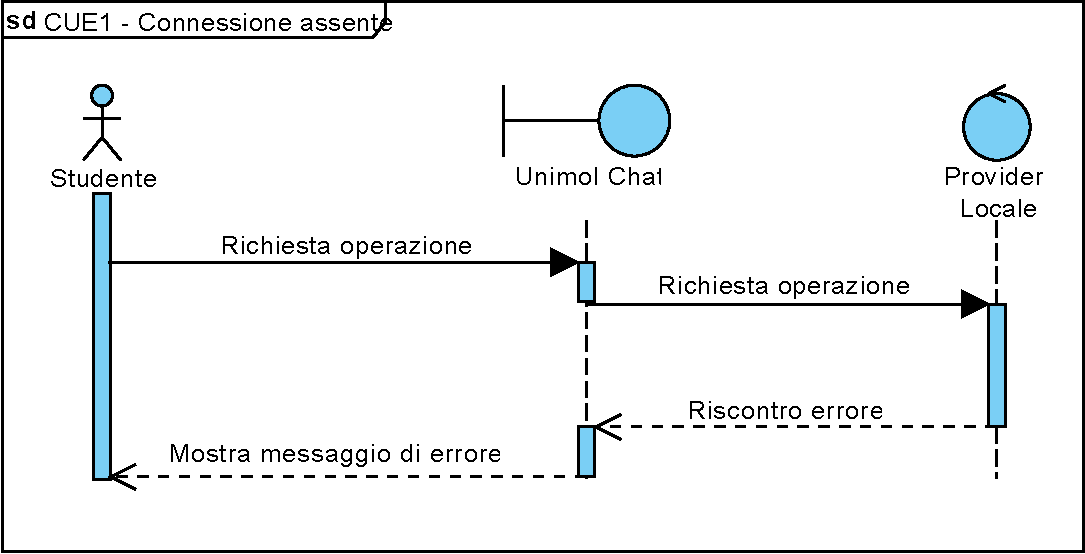
\includegraphics[width=0.9\textwidth]{imgs/gruppo6/sequence/CUE1_connessione_assente.pdf}
	\caption{CUE1 - Connessione assente}
	\label{fig:seq-cue1}
\end{figure}


\begin{figure}
	\centering
	\includegraphics[width=0.9\textwidth]{imgs/gruppo6/sequence/CUE2_nessuna_risposta_dal_server.pdf}
	\caption{CUE2 - Nessuna risposta dal server}
	\label{fig:seq-cue2}
\end{figure}

\clearpage
\subsection{Funzionalità rubrica}
\begin{figure}[H]
	\centering
	\includegraphics[width=0.9\textwidth]{imgs/gruppo5/sequence1.pdf}
	\caption{Ricerca non filtarta}
	\label{fig:seq1-rubrica}
\end{figure}

\begin{figure}[H]
\centering
\includegraphics[width=0.9\textwidth]{imgs/gruppo5/sequence2.pdf}
\caption{Ricerca filtarta}
\label{fig:seq2-rubrica}
\end{figure}

\begin{figure}[H]
	\centering
	\includegraphics[width=0.9\textwidth]{imgs/gruppo5/sequence3.pdf}
	\caption{Visualizza contatto}
	\label{fig:seq3-rubrica}
\end{figure}

\clearpage
\subsection{Funzionalità previsione media}
\begin{figure}[H]
	\centering
	\includegraphics[width=0.9\textwidth]{imgs/gruppo3/sequence-media-valori-validi.pdf}
	\caption{sequence simulazione media}
	\label{fig:seq1-media}
\end{figure}

\begin{figure}[H]
	\centering
	\includegraphics[width=0.9\textwidth]{imgs/gruppo3/sequence-media-valori-non-validi.pdf}
	\caption{Sequence simulazione media con valori non validi o vuoti}
	\label{fig:seq2-media}
\end{figure}

\begin{figure}[H]
	\centering
	\includegraphics[width=0.9\textwidth]{imgs/gruppo3/sequence-media-esami-finiti.pdf}
	\caption{Sequence simulazione media con esami finiti}
	\label{fig:seq3-media}
\end{figure}

\section{Diagramma delle attività}

\subsection{Funzionalità chat}

%%% START activities chat studenti %%%
\begin{figure}[!h]
	\subsubsection{Chat studenti}
	\centering
	\includegraphics[width=0.9\textwidth]{imgs/gruppo6/activities/act_cus1_visualizza_canale.pdf}
	\caption{CUS 1 - Visualizza canale}
	\label{fig:act-cus1}
\end{figure}

\begin{figure}
	\centering
	\includegraphics[width=0.9\textwidth]{imgs/gruppo6/activities/act_cus2_invio_messaggio.pdf}
	\caption{CUS2 - Invio messaggio}
	\label{fig:act-cus2}
\end{figure}

\begin{figure}
	\centering
	\includegraphics[width=0.9\textwidth]{imgs/gruppo6/activities/act_cus3_invia_allegato.pdf}
	\caption{CUS3 - Invio Allegato}
	\label{fig:act-cus3-1}
\end{figure}

\begin{figure}
	\centering
	\includegraphics[width=0.9\textwidth]{imgs/gruppo6/activities/act_cus3_invio_allegato2.pdf}
	\caption{CUS3 - Invio Allegato (es. 2)}
	\label{fig:act-cus3-2}
\end{figure}

\begin{figure}
	\centering
	\includegraphics[width=0.9\textwidth]{imgs/gruppo6/activities/act_cus4_rispondi_singolo_messaggio.pdf}
	\caption{CUS4 - Rispondi al messaggio}
	\label{fig:act-cus4}
\end{figure}

\begin{figure}
	\centering
	\includegraphics[width=0.9\textwidth]{imgs/gruppo6/activities/act_cus5_scarica_allegato.pdf}
	\caption{CUS5 - Scarica allegato}
	\label{fig:act-cus5}
\end{figure}

\begin{figure}
	\centering
	\includegraphics[width=0.9\textwidth]{imgs/gruppo6/activities/act_cus6_segnalazione_messaggio.pdf}
	\caption{CUS6 - Segnalazione messaggio}
	\label{fig:act-cus6}
\end{figure}

\begin{figure}
	\centering
	\includegraphics[width=0.9\textwidth]{imgs/gruppo6/activities/act_cus7_ricerca_testo_nella_chat.pdf}
	\caption{CUS7 - Ricerca testo nella chat}
	\label{fig:act-cus7}
\end{figure}

\begin{figure}
	\centering
	\includegraphics[width=0.9\textwidth]{imgs/gruppo6/activities/act_cus8_tag_membro_messaggio.pdf}
	\caption{CUS8 - Tag membro in messaggio}
	\label{fig:act-cus8}
\end{figure}

\begin{figure}
	\centering
	\includegraphics[width=0.9\textwidth]{imgs/gruppo6/activities/act_cus9_gestisci_notifiche_chat.pdf}
	\caption{CUS9 - Gestisci notifiche chat}
	\label{fig:act-cus9}
\end{figure}

\begin{figure}
	\centering
	\includegraphics[width=0.9\textwidth]{imgs/gruppo6/activities/act_cus10_seleziona_emoji.pdf}
	\caption{CUS10 - Selezione emoji}
	\label{fig:act-cus10}
\end{figure}

\begin{figure}
	\centering
	\includegraphics[width=0.9\textwidth]{imgs/gruppo6/activities/act_cus11_elenco_membri.pdf}
	\caption{CUS11 - Visualizza elenco membri chat}
	\label{fig:act-cus11}
\end{figure}
%%% END activities chat studenti %%%

%%% START activities chat docenti %%%
\pagebreak
\begin{figure}[!h]
	\subsubsection{Chat docenti}
	\centering
	\includegraphics[width=0.9\textwidth]{imgs/gruppo6/activities/act_cud1_creazione_canale.pdf}
	\caption{CUD1 - Creazione canale}
	\label{fig:act-cud1}
\end{figure}

\begin{figure}
	\centering
	\includegraphics[width=0.9\textwidth]{imgs/gruppo6/activities/act_cud2_cancella_canale.pdf}
	\caption{CUD2 - Cancellazione canale}
	\label{fig:act-cud2}
\end{figure}

\begin{figure}
	\centering
	\includegraphics[width=0.9\textwidth]{imgs/gruppo6/activities/act_cud3_aggiungi_membro_chat.pdf}
	\caption{CUD3 - Aggiungi membro ad un canale}
	\label{fig:act-cud3}
\end{figure}

\begin{figure}
	\centering
	\includegraphics[width=0.9\textwidth]{imgs/gruppo6/activities/act_cud4_rimuovi_membro_da_canale.pdf}
	\caption{CUD4 - Rimuovi membro da un canale}
	\label{fig:act-cud4}
\end{figure}

\begin{figure}
	\centering
	\includegraphics[width=0.9\textwidth]{imgs/gruppo6/activities/act_cud5_blocca_studente.pdf}
	\caption{CUD5 - Blocca Studente}
	\label{fig:act-cud5}
\end{figure}

\begin{figure}
	\centering
	\includegraphics[width=0.9\textwidth]{imgs/gruppo6/activities/act_cud5_blocca_studente2.pdf}
	\caption{CUD5 - Blocca Studente (es. 2}
	\label{fig:act-cud5-2}
\end{figure}

\begin{figure}
	\centering
	\includegraphics[width=0.9\textwidth]{imgs/gruppo6/activities/act_cud6_sblocca_da_elenco.pdf}
	\caption{CUD6 - Sblocca Studente (da elenco)}
	\label{fig:act-cud6}
\end{figure}

\begin{figure}
	\centering
	\includegraphics[width=0.9\textwidth]{imgs/gruppo6/activities/act_cud6_sblocca_da_messaggio.pdf}
	\caption{CUD6 - Sblocca Studente (da messaggio)}
	\label{fig:act-cud6-2}
\end{figure}
%%% END activities chat docenti %%%

%%% START activities chat pannello %%%
\pagebreak
\begin{figure}[!h]
	\subsubsection{Pannello di amministrazione}
	\centering
	\includegraphics[width=0.9\textwidth]{imgs/gruppo6/activities/act_cup1_login.pdf}
	\caption{CUP1 - Login}
	\label{fig:act-cup1}
\end{figure}

\begin{figure}
	\centering
	\includegraphics[width=0.9\textwidth]{imgs/gruppo6/activities/act_cup2_logout.pdf}
	\caption{CUP2 - Logout}
	\label{fig:act-cup2}
\end{figure}

\begin{figure}
	\centering
	\includegraphics[width=0.9\textwidth]{imgs/gruppo6/activities/act_cup3_filtro_chat_corsi1.pdf}
	\caption{CUP3 - Ricerca chat (filtri chat corsi - pt.1)}
	\label{fig:act-cup3}
\end{figure}

\begin{figure}
	\centering
	\includegraphics[width=0.9\textwidth]{imgs/gruppo6/activities/act_cup3_filtro_chat_corsi2.pdf}
	\caption{CUP3 - Ricerca chat (filtri chat corsi - pt.2)}
	\label{fig:act-cup3-2}
\end{figure}

\begin{figure}
	\centering
	\includegraphics[width=0.9\textwidth]{imgs/gruppo6/activities/act_cup3_filtro_chat_studenti1.pdf}
	\caption{CUP3 - Ricerca chat (filtri chat studenti - pt.1)}
	\label{fig:act-cup3-3}
\end{figure}

\begin{figure}
	\centering
	\includegraphics[width=0.9\textwidth]{imgs/gruppo6/activities/act_cup3_filtro_chat_studenti2.pdf}
	\caption{CUP3 - Ricerca chat (filtri chat studenti - pt.2)}
	\label{fig:act-cup3-4}
\end{figure}

\begin{figure}
	\centering
	\includegraphics[width=0.9\textwidth]{imgs/gruppo6/activities/act_cup3_ricerca_chat_corsi1.pdf}
	\caption{CUP3 - Ricerca chat (cerca corsi - pt.1)}
	\label{fig:act-cup3-5}
\end{figure}

\begin{figure}
	\centering
	\includegraphics[width=0.9\textwidth]{imgs/gruppo6/activities/act_cup3_ricerca_chat_corsi2.pdf}
	\caption{CUP3 - Ricerca chat (cerca corsi - pt.2)}
	\label{fig:act-cup3-6}
\end{figure}

\begin{figure}
	\centering
	\includegraphics[width=0.9\textwidth]{imgs/gruppo6/activities/act_cup3_ricerca_chat_studenti.pdf}
	\caption{CUP3 - Ricerca chat (cerca studenti - pt.1)}
	\label{fig:act-cup3-7}
\end{figure}

\begin{figure}
	\centering
	\includegraphics[width=0.9\textwidth]{imgs/gruppo6/activities/act_cup3_ricerca_chat_studenti2.pdf}
	\caption{CUP3 - Ricerca chat (cerca studenti - pt.2)}
	\label{fig:act-cup3-8}
\end{figure}

\begin{figure}
	\centering
	\includegraphics[width=0.9\textwidth]{imgs/gruppo6/activities/act_cup4_visualizza_lista_chat_corsi1.pdf}
	\caption{CUP4 - Visualizza lista chat (corsi - pt.1)}
	\label{fig:act-cup4}
\end{figure}

\begin{figure}
	\centering
	\includegraphics[width=0.9\textwidth]{imgs/gruppo6/activities/act_cup4_visualizza_lista_chat_corsi2.pdf}
	\caption{CUP4 - Visualizza lista chat (corsi - pt.2)}
	\label{fig:act-cup4-2}
\end{figure}

\begin{figure}
	\centering
	\includegraphics[width=0.9\textwidth]{imgs/gruppo6/activities/act_cup4_visualizza_lista_chat_studenti.pdf}
	\caption{CUP4 - Visualizza lista chat (studenti)}
	\label{fig:act-cup4-3}
\end{figure}

\begin{figure}
	\centering
	\includegraphics[width=0.9\textwidth]{imgs/gruppo6/activities/act_cup5_abilita_chat.pdf}
	\caption{CUP5 - Abilita chat}
	\label{fig:act-cup5}
\end{figure}

\begin{figure}
	\centering
	\includegraphics[width=0.9\textwidth]{imgs/gruppo6/activities/act_cup6_disabilita_chat.pdf}
	\caption{CUP6 - Disabilita chat}
	\label{fig:act-cup6}
\end{figure}

\begin{figure}
	\centering
	\includegraphics[width=0.9\textwidth]{imgs/gruppo6/activities/act_cup7_visualizza_canale.pdf}
	\caption{CUP7 - Visualizza canale}
	\label{fig:act-cup7}
\end{figure}

\begin{figure}
	\centering
	\includegraphics[width=0.9\textwidth]{imgs/gruppo6/activities/act_cup8_aggiungi_canale1.pdf}
	\caption{CUP8 - Aggiungi canale (pt.1)}
	\label{fig:act-cup8}
\end{figure}

\begin{figure}
	\centering
	\includegraphics[width=0.9\textwidth]{imgs/gruppo6/activities/act_cup8_aggiungi_canale2.pdf}
	\caption{CUP8 - Aggiungi canale (pt.2)}
	\label{fig:act-cup8-2}
\end{figure}

\begin{figure}
	\centering
	\includegraphics[width=0.9\textwidth]{imgs/gruppo6/activities/act_cup9_cancella_canale1.pdf}
	\caption{CUP9 - Cancella canale (pt.1)}
	\label{fig:act-cup9}
\end{figure}

\begin{figure}
	\centering
	\includegraphics[width=0.9\textwidth]{imgs/gruppo6/activities/act_cup9_cancella_canale2.pdf}
	\caption{CUP9 - Cancella canale (pt.2)}
	\label{fig:act-cup9-2}
\end{figure}

\begin{figure}
	\centering
	\includegraphics[width=0.9\textwidth]{imgs/gruppo6/activities/act_cup10_visualizza_lista_utenti.pdf}
	\caption{CUP10 - Visualizza lista utenti}
	\label{fig:act-cup10}
\end{figure}

\begin{figure}
	\centering
	\includegraphics[width=0.9\textwidth]{imgs/gruppo6/activities/act_cup11_aggiungi_utente_canale1.pdf}
	\caption{CUP11 - Aggiungi un utente ad un canale (pt.1)}
	\label{fig:act-cup11}
\end{figure}

\begin{figure}
	\centering
	\includegraphics[width=0.9\textwidth]{imgs/gruppo6/activities/act_cup11_aggiungi_utente_canale2.pdf}
	\caption{CUP11 - Aggiungi un utente ad un canale (pt.2)}
	\label{fig:act-cup11-2}
\end{figure}

\begin{figure}
	\centering
	\includegraphics[width=0.9\textwidth]{imgs/gruppo6/activities/act_cup12_cancella_utente_canale.pdf}
	\caption{CUP12 - Rimuovere un utente da un canale}
	\label{fig:act-cup12}
\end{figure}

\begin{figure}
	\centering
	\includegraphics[width=0.9\textwidth]{imgs/gruppo6/activities/act_cup13_silenziare_utente1.pdf}
	\caption{CUP13 - Silenziare utente in un canale (pt.1)}
	\label{fig:act-cup13}
\end{figure}

\begin{figure}
	\centering
	\includegraphics[width=0.9\textwidth]{imgs/gruppo6/activities/act_cup13_silenziare_utente2.pdf}
	\caption{CUP13 - Silenziare utente in un canale (pt.2)}
	\label{fig:act-cup13-2}
\end{figure}

\begin{figure}
	\centering
	\includegraphics[width=0.9\textwidth]{imgs/gruppo6/activities/act_cup14_reintegra_utente.pdf}
	\caption{CUP14 - Reintegra utente in un canale}
	\label{fig:act-cup14}
\end{figure}

\begin{figure}
	\centering
	\includegraphics[width=0.9\textwidth]{imgs/gruppo6/activities/act_cup15_modifica_permessi_utente1.pdf}
	\caption{CUP15 - Modificare i permessi di un utente in un canale (pt.1)}
	\label{fig:act-cup15-1}
\end{figure}

\begin{figure}
	\centering
	\includegraphics[width=0.9\textwidth]{imgs/gruppo6/activities/act_cup15_modifica_permessi_utente2.pdf}
	\caption{CUP15 - Modificare i permessi di un utente in un canale (pt.2)}
	\label{fig:act-cup15-2}
\end{figure}

\begin{figure}
	\centering
	\includegraphics[width=0.9\textwidth]{imgs/gruppo6/activities/act_cup16_nascondi_messaggio.pdf}
	\caption{CUP16 - Nascondi messaggio}
	\label{fig:act-cup16}
\end{figure}

\begin{figure}
	\centering
	\includegraphics[width=0.9\textwidth]{imgs/gruppo6/activities/act_cup17_reintegra_messaggio.pdf}
	\caption{CUP17  - Reintegra messaggio}
	\label{fig:act-cup17}
\end{figure}

\begin{figure}
	\centering
	\includegraphics[width=0.9\textwidth]{imgs/gruppo6/activities/act_cup18_invio_notifiche1.pdf}
	\caption{CUP18 - Invio Notifiche (pt.1)}
	\label{fig:act-cup18}
\end{figure}

\begin{figure}
	\centering
	\includegraphics[width=0.9\textwidth]{imgs/gruppo6/activities/act_cup18_invio_notifiche2.pdf}
	\caption{CUP18 - Invio Notifiche (pt.2)}
	\label{fig:act-cup18-2}
\end{figure}

\begin{figure}
	\centering
	\includegraphics[width=0.9\textwidth]{imgs/gruppo6/activities/act_cup19_gestione_messaggi_inopportuni.pdf}
	\caption{CUP19 - Gestione messaggi inopportuni}
	\label{fig:act-cup19}
\end{figure}
%%% END activities chat pannello %%%

\clearpage
\subsection{Funzionalità rubrica}
\begin{figure}[H]
	\centering
	\includegraphics[width=0.9\textwidth]{imgs/gruppo5/activity.pdf}
	\caption{Rubrica}
	\label{fig:act-rubrica}
\end{figure}

\clearpage
\subsection{Funzionalità previsione media}
\begin{figure}[H]
	\centering
	\includegraphics[width=0.9\textwidth]{imgs/gruppo3/media-activity-diagram.pdf}
	\caption{Diagramma di attività}
	\label{fig:act-rubrica}
\end{figure}

\clearpage